\documentclass[]{book}
\usepackage{lmodern}
\usepackage{amssymb,amsmath}
\usepackage{ifxetex,ifluatex}
\usepackage{fixltx2e} % provides \textsubscript
\ifnum 0\ifxetex 1\fi\ifluatex 1\fi=0 % if pdftex
  \usepackage[T1]{fontenc}
  \usepackage[utf8]{inputenc}
\else % if luatex or xelatex
  \ifxetex
    \usepackage{mathspec}
  \else
    \usepackage{fontspec}
  \fi
  \defaultfontfeatures{Ligatures=TeX,Scale=MatchLowercase}
\fi
% use upquote if available, for straight quotes in verbatim environments
\IfFileExists{upquote.sty}{\usepackage{upquote}}{}
% use microtype if available
\IfFileExists{microtype.sty}{%
\usepackage{microtype}
\UseMicrotypeSet[protrusion]{basicmath} % disable protrusion for tt fonts
}{}
\usepackage{hyperref}
\hypersetup{unicode=true,
            pdftitle={Power Analysis with Superpower},
            pdfauthor={Aaron R. Caldwell \& Daniël Lakens},
            pdfborder={0 0 0},
            breaklinks=true}
\urlstyle{same}  % don't use monospace font for urls
\usepackage{natbib}
\bibliographystyle{apalike}
\usepackage{color}
\usepackage{fancyvrb}
\newcommand{\VerbBar}{|}
\newcommand{\VERB}{\Verb[commandchars=\\\{\}]}
\DefineVerbatimEnvironment{Highlighting}{Verbatim}{commandchars=\\\{\}}
% Add ',fontsize=\small' for more characters per line
\usepackage{framed}
\definecolor{shadecolor}{RGB}{248,248,248}
\newenvironment{Shaded}{\begin{snugshade}}{\end{snugshade}}
\newcommand{\AlertTok}[1]{\textcolor[rgb]{0.94,0.16,0.16}{#1}}
\newcommand{\AnnotationTok}[1]{\textcolor[rgb]{0.56,0.35,0.01}{\textbf{\textit{#1}}}}
\newcommand{\AttributeTok}[1]{\textcolor[rgb]{0.77,0.63,0.00}{#1}}
\newcommand{\BaseNTok}[1]{\textcolor[rgb]{0.00,0.00,0.81}{#1}}
\newcommand{\BuiltInTok}[1]{#1}
\newcommand{\CharTok}[1]{\textcolor[rgb]{0.31,0.60,0.02}{#1}}
\newcommand{\CommentTok}[1]{\textcolor[rgb]{0.56,0.35,0.01}{\textit{#1}}}
\newcommand{\CommentVarTok}[1]{\textcolor[rgb]{0.56,0.35,0.01}{\textbf{\textit{#1}}}}
\newcommand{\ConstantTok}[1]{\textcolor[rgb]{0.00,0.00,0.00}{#1}}
\newcommand{\ControlFlowTok}[1]{\textcolor[rgb]{0.13,0.29,0.53}{\textbf{#1}}}
\newcommand{\DataTypeTok}[1]{\textcolor[rgb]{0.13,0.29,0.53}{#1}}
\newcommand{\DecValTok}[1]{\textcolor[rgb]{0.00,0.00,0.81}{#1}}
\newcommand{\DocumentationTok}[1]{\textcolor[rgb]{0.56,0.35,0.01}{\textbf{\textit{#1}}}}
\newcommand{\ErrorTok}[1]{\textcolor[rgb]{0.64,0.00,0.00}{\textbf{#1}}}
\newcommand{\ExtensionTok}[1]{#1}
\newcommand{\FloatTok}[1]{\textcolor[rgb]{0.00,0.00,0.81}{#1}}
\newcommand{\FunctionTok}[1]{\textcolor[rgb]{0.00,0.00,0.00}{#1}}
\newcommand{\ImportTok}[1]{#1}
\newcommand{\InformationTok}[1]{\textcolor[rgb]{0.56,0.35,0.01}{\textbf{\textit{#1}}}}
\newcommand{\KeywordTok}[1]{\textcolor[rgb]{0.13,0.29,0.53}{\textbf{#1}}}
\newcommand{\NormalTok}[1]{#1}
\newcommand{\OperatorTok}[1]{\textcolor[rgb]{0.81,0.36,0.00}{\textbf{#1}}}
\newcommand{\OtherTok}[1]{\textcolor[rgb]{0.56,0.35,0.01}{#1}}
\newcommand{\PreprocessorTok}[1]{\textcolor[rgb]{0.56,0.35,0.01}{\textit{#1}}}
\newcommand{\RegionMarkerTok}[1]{#1}
\newcommand{\SpecialCharTok}[1]{\textcolor[rgb]{0.00,0.00,0.00}{#1}}
\newcommand{\SpecialStringTok}[1]{\textcolor[rgb]{0.31,0.60,0.02}{#1}}
\newcommand{\StringTok}[1]{\textcolor[rgb]{0.31,0.60,0.02}{#1}}
\newcommand{\VariableTok}[1]{\textcolor[rgb]{0.00,0.00,0.00}{#1}}
\newcommand{\VerbatimStringTok}[1]{\textcolor[rgb]{0.31,0.60,0.02}{#1}}
\newcommand{\WarningTok}[1]{\textcolor[rgb]{0.56,0.35,0.01}{\textbf{\textit{#1}}}}
\usepackage{longtable,booktabs}
\usepackage{graphicx,grffile}
\makeatletter
\def\maxwidth{\ifdim\Gin@nat@width>\linewidth\linewidth\else\Gin@nat@width\fi}
\def\maxheight{\ifdim\Gin@nat@height>\textheight\textheight\else\Gin@nat@height\fi}
\makeatother
% Scale images if necessary, so that they will not overflow the page
% margins by default, and it is still possible to overwrite the defaults
% using explicit options in \includegraphics[width, height, ...]{}
\setkeys{Gin}{width=\maxwidth,height=\maxheight,keepaspectratio}
\IfFileExists{parskip.sty}{%
\usepackage{parskip}
}{% else
\setlength{\parindent}{0pt}
\setlength{\parskip}{6pt plus 2pt minus 1pt}
}
\setlength{\emergencystretch}{3em}  % prevent overfull lines
\providecommand{\tightlist}{%
  \setlength{\itemsep}{0pt}\setlength{\parskip}{0pt}}
\setcounter{secnumdepth}{5}
% Redefines (sub)paragraphs to behave more like sections
\ifx\paragraph\undefined\else
\let\oldparagraph\paragraph
\renewcommand{\paragraph}[1]{\oldparagraph{#1}\mbox{}}
\fi
\ifx\subparagraph\undefined\else
\let\oldsubparagraph\subparagraph
\renewcommand{\subparagraph}[1]{\oldsubparagraph{#1}\mbox{}}
\fi

%%% Use protect on footnotes to avoid problems with footnotes in titles
\let\rmarkdownfootnote\footnote%
\def\footnote{\protect\rmarkdownfootnote}

%%% Change title format to be more compact
\usepackage{titling}

% Create subtitle command for use in maketitle
\providecommand{\subtitle}[1]{
  \posttitle{
    \begin{center}\large#1\end{center}
    }
}

\setlength{\droptitle}{-2em}

  \title{Power Analysis with Superpower}
    \pretitle{\vspace{\droptitle}\centering\huge}
  \posttitle{\par}
    \author{Aaron R. Caldwell \& Daniël Lakens}
    \preauthor{\centering\large\emph}
  \postauthor{\par}
      \predate{\centering\large\emph}
  \postdate{\par}
    \date{2019-09-27}

\usepackage{booktabs}
\usepackage{booktabs}
\usepackage{longtable}
\usepackage{array}
\usepackage{multirow}
\usepackage{wrapfig}
\usepackage{float}
\usepackage{colortbl}
\usepackage{pdflscape}
\usepackage{tabu}
\usepackage{threeparttable}
\usepackage{threeparttablex}
\usepackage[normalem]{ulem}
\usepackage{makecell}
\usepackage{xcolor}

\begin{document}
\maketitle

{
\setcounter{tocdepth}{1}
\tableofcontents
}
This is a compilation of documents for \href{https://github.com/arcaldwell49/Superpower}{Superpower} R package written in \textbf{Markdown} \citep{R-rmarkdown} and compiled by \textbf{Bookdown} \citep{R-bookdown}.

\hypertarget{preface}{%
\chapter*{Preface}\label{preface}}
\addcontentsline{toc}{chapter}{Preface}

The goal of \texttt{Superpower} is to easily simulate factorial designs and empirically calculate power using a simulation approach.
The R package is intended to be utilized for prospective (a priori) power analysis. Please don't be silly and compute \href{https://discourse.datamethods.org/t/reference-collection-to-push-back-against-common-statistical-myths/1787}{post hoc power}.

This package, and book, expect readers to have some familiarity with R \citeyearpar{R-base}. However, we have created two Shiny apps (for the \href{http://shiny.ieis.tue.nl/anova_power/}{\texttt{ANOVA\_power}} \& \href{http://shiny.ieis.tue.nl/anova_exact/}{\texttt{ANOVA\_exact}} functions respectively) to help use these functions if you are not familiar with R.

In this book we will display a variety of ways the \texttt{Superpower} package can be used for power analysis and sample size planning for factorial experimental designs. We also included various examples of the performance of \texttt{Superpower} against other R packages (e.g., \texttt{pwr2ppl} by \citet{R-pwr2ppl} and \texttt{pwr} by \citet{R-pwr}) and statistical programs (such as G*Power \citet{faul2007g}, MOREpower \citet{Campbell2012MorePower6F}, and SAS's \texttt{PROC\ GLMPOWER} \citeyearpar{SASglmpower}). All uses of the \texttt{ANOVA\_power} function have been run with 10000 iterations (\texttt{nsims\ =\ 10000}). If you have any issues using \texttt{Superpower} or want to expand its capabilities please raise the issue on our \href{https://github.com/arcaldwell49/Superpower/issues}{GitHub} repository.

\hypertarget{the-experimental-design}{%
\chapter{The Experimental Design}\label{the-experimental-design}}

This section introduces how \texttt{Superpower} allows the user to specify their experimental design.
Currently, this pacakge only provides power analysis for ANOVAs (and MANOVA for repeated measures) so all designs are currently defined by the \texttt{ANOVA\_design} function.

\hypertarget{anova_design-function}{%
\section{ANOVA\_design function}\label{anova_design-function}}

Currently the \texttt{ANOVA\_design} function can create designs with up to three factors, for both within, between, and mixed designs. It requires the following input: design, n, mu, sd, r, and optionally allows you to set labelnames.

\begin{enumerate}
\def\labelenumi{\arabic{enumi}.}
\tightlist
\item
  \texttt{design}: string that specifies the design (see below).
\item
  \texttt{n}: the sample size for each between subject condition.
\item
  \texttt{mu}: a vector with the means for each condition.
\item
  \texttt{sd}: the population standard deviation. Assumes homogeneity of variances (only one standard deviation can be provided).
\item
  \texttt{r}: the correlation(s) for within designs (or 0 for between designs).
\item
  \texttt{labelnames}: This is an optonal vector of words that indicates factor names and level names (see below).
\item
  A final optional setting is to specify if you want to automatically print a plot or not (\texttt{plot} = TRUE or FALSE)
\end{enumerate}

\hypertarget{specifying-the-design-using-design}{%
\subsection{\texorpdfstring{Specifying the design using \texttt{design}}{Specifying the design using design}}\label{specifying-the-design-using-design}}

The \texttt{design} option is used to specify the design.
Every factor is specified with a number, indicating the number of levels of the factor, and a letter, b or w, to indicate whether the factor is manipulated between or within participants.
For example, a \texttt{2b} design has two between-participant groups.
A \texttt{12w} design has one factor with 12 levels, all manipulated within-participants.
A \texttt{2b*3w} is a design with two factors (a 2b factor and a 3w factor), the first of which has 2 between participant levels (2b), and the second of which has 3 within participants levels (3w).
\textbf{If there are multiple factors (the functions take up to three different factors) separate factors with a * (asterisk)}.
An example of a \texttt{2b*3w} design is a group of people in one condition who get a drug, and a group of people in another condition who get a placebo (hence \texttt{2b}), and we measure their health before they take the pill, one day after they take the pill, and a week after they take the pill (hence the \texttt{3w}).

\hypertarget{specifying-the-means-using-mu}{%
\subsection{\texorpdfstring{Specifying the means using \texttt{mu}}{Specifying the means using mu}}\label{specifying-the-means-using-mu}}

Note that for each cell in the design, a mean must be provided. Thus, for a \texttt{2b*3w} design, \textbf{6} (i.e., 2*3=6) means need to be entered.

Means need to be entered in the correct order. ANOVA\_design outputs a plot so you can check if you entered all means as you intended. Always carefully check if the plot that is generated matches your expectations.

The general principle is that the code generates factors, indicated by the factor names you entered in the labelnames variable, (i.e., \emph{condition} and \emph{time}). Levels are indicated by factor names and levels (e.g., control\_time1, control\_time2, control\_time3, etc).

If your design has just one factor, just enter the means in the same order as the labelnames (see below). For more factors, note the general pattern in the example below. Means are entered in the following order for a 3 factors design (each with 2 levels):

\begin{enumerate}
\def\labelenumi{\arabic{enumi}.}
\tightlist
\item
  a1 b1 c1
\item
  a1 b1 c2
\item
  a1 b2 c1
\item
  a1 b2 c2
\item
  a2 b1 c1
\item
  a2 b1 c2
\item
  a2 b2 c1
\item
  a2 b2 c2
\end{enumerate}

So if you enter the means 1, 2, 3, 4, 5, 6, 7, 8 the first 4 means correspond to level 1 of factor 1, the second 4 means correspond to level 2 of factor 1. Within the first 4 means, the first 2 correspond to level 1 of factor 2, and within those 2 means, the first corresponds to level 1 of factor 3.

The plot below visualizes means from 1 to 8 being entered in a vector: \texttt{mu\ =\ c(1,\ 2,\ 3,\ 4,\ 5,\ 6,\ 7,\ 8)} so you can see how the basic ordering works.

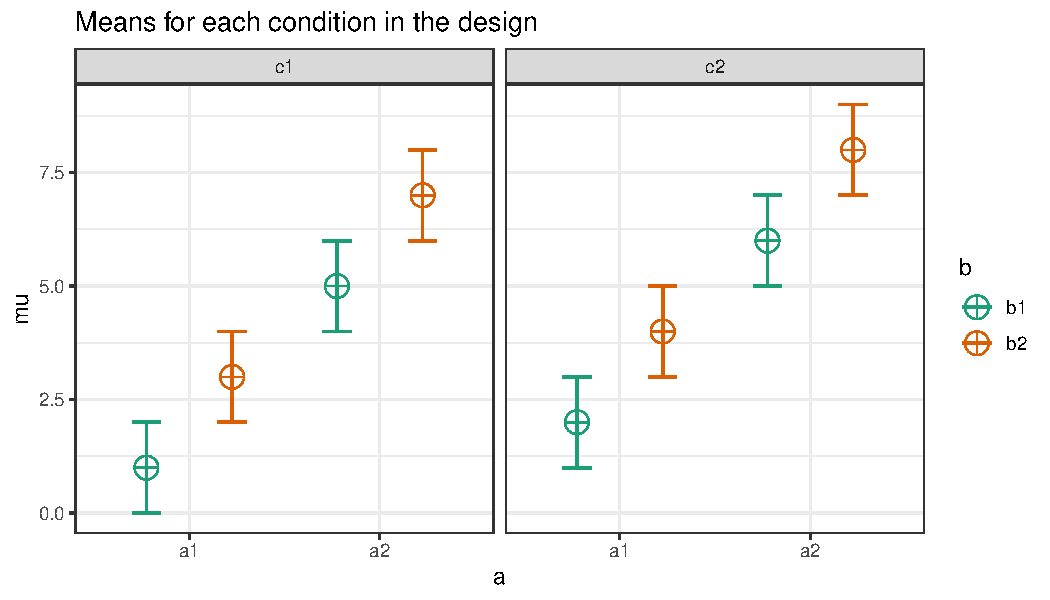
\includegraphics{SuperpowerValidation_files/figure-latex/unnamed-chunk-2-1.pdf}

\hypertarget{specifying-label-names}{%
\subsection{Specifying label names}\label{specifying-label-names}}

To make sure the plots and tables with simulation results are easy to interpret, it really helps to name all factors and levels. You can enter the labels in the `labelnames' variable. You can also choose not to specify names. Then all factors are indicated by letters (a, b, c) and all levels by numbers (a1, a2, a3).

For the 2x3 design we have been using as an example, where there are 2 factors (condition and time of measurement), the first with 2 levels (placebo vs.~medicine) and the second with three levels (time1, time2, and time3) we would enter the labels as follows:

\texttt{c("condition",\ "placebo",\ "medicine",\ "time",\ "time1",\ "time2",\ "time3")}

As you can see, you follow the order of the design (\texttt{2b*3w}), and first write the \textbf{FACTOR} label (condition) followed by the levels of that factor (placebo and medicine). Then you write the second factor name (time) followed by the three labels for each \textbf{LEVEL} (time1, time2, time3). \textbf{Do not use spaces or special characters in the names (so not ``time 1'' or ``time\_1'' but ``time1'').}

Some examples:

\begin{enumerate}
\def\labelenumi{\arabic{enumi}.}
\tightlist
\item
  One within factor (time with 2 levels), 2w:
  \texttt{c("time",\ "morning",\ "evening")}
\item
  Two between factors (time and group, each with 2 levels), 2b*2b:
  \texttt{c("time",\ "morning",\ "evening",\ "group",\ "control",\ "experimental")}
\item
  Two between factors (time and group, first with 4 levels, second with 2 levels), 4b*2b:
  \texttt{c("time",\ "morning",\ "afternoon"\ ,"evening",\ "night",\ "group",\ "control",\ "experimental")}
\end{enumerate}

\hypertarget{specifying-the-correlation}{%
\subsection{Specifying the correlation}\label{specifying-the-correlation}}

Depending on whether factors are manipulated within or between, variables are correlated, or not. You can set the correlation for within-participant factors. You can either assume all factors have the same correlation (e.g., r = 0.7), or enter the correlations for each pair of observations separately by specifying a correlation matrix.

In a 2x2 design, with factors A and B, each with 2 levels, there are 6 possible comparisons that can be made.

\begin{enumerate}
\def\labelenumi{\arabic{enumi}.}
\tightlist
\item
  A1 vs.~A2
\item
  A1 vs.~B1
\item
  A1 vs.~B2
\item
  A2 vs.~B1
\item
  A2 vs.~B2
\item
  B1 vs.~B2
\end{enumerate}

The number of possible comparisons is the product of the levels of all factors squared minus the product of all factors, divided by two. For a 2x2 design where each factor has two levels, this is:

\begin{Shaded}
\begin{Highlighting}[]
\NormalTok{(((}\DecValTok{2} \OperatorTok{*}\StringTok{ }\DecValTok{2}\NormalTok{) }\OperatorTok{^}\StringTok{ }\DecValTok{2}\NormalTok{) }\OperatorTok{-}\StringTok{ }\NormalTok{(}\DecValTok{2} \OperatorTok{*}\StringTok{ }\DecValTok{2}\NormalTok{))}\OperatorTok{/}\DecValTok{2}
\end{Highlighting}
\end{Shaded}

\begin{verbatim}
## [1] 6
\end{verbatim}

The number of possible comparisons increases rapidly when adding factors and levels for each factor. For example, for a 2x2x4 design it is:

\begin{Shaded}
\begin{Highlighting}[]
\NormalTok{(((}\DecValTok{2} \OperatorTok{*}\StringTok{ }\DecValTok{2} \OperatorTok{*}\StringTok{ }\DecValTok{4}\NormalTok{) }\OperatorTok{^}\StringTok{ }\DecValTok{2}\NormalTok{) }\OperatorTok{-}\StringTok{ }\NormalTok{(}\DecValTok{2} \OperatorTok{*}\StringTok{ }\DecValTok{2} \OperatorTok{*}\StringTok{ }\DecValTok{4}\NormalTok{))}\OperatorTok{/}\DecValTok{2}
\end{Highlighting}
\end{Shaded}

\begin{verbatim}
## [1] 120
\end{verbatim}

Each of these comparisons can have their own correlation if the factor is manipulated within subjects (if the factor is manipulated between subjects the correlation is 0). These correlations determine the covariance matrix. Potvin and Schutz (2000) surveyed statistical tools for power analysis and conclude that most software packages are limited to one factor repeated measure designs and do not provide power calculations for within designs with multiple factor (which is still true for software such as G*Power). Furthermore, software solutions which were available at the time (DATASIM by Bradley, Russel, \& Reeve, 1996) required researchers to assume correlations were of the same magnitude for all within factors, which is not always realistic. If you do not want to assume equal correlations for all paired comparisons, you can specify the correlation for each possible comparison.

The order in which the correlations are entered in the vector should match the covariance matrix.
The order for a 2x2 design is given in the 6 item list above. The general pattern is that the matrix is filled from top to bottom, and left to right, illustrated by the increasing correlations in the table below.
The diagonal is generated dynamically (based on the standard deviation).

\begin{longtable}[]{@{}lllll@{}}
\toprule
Matrix & a1\_b1 & a1\_b2 & a2\_b1 & a2\_b2\tabularnewline
\midrule
\endhead
a1\_b1 & 1.00 & 0.91 & 0.92 & 0.93\tabularnewline
a1\_b2 & 0.91 & 1.00 & 0.94 & 0.95\tabularnewline
a2\_b1 & 0.92 & 0.94 & 1.00 & 0.96\tabularnewline
a2\_b2 & 0.93 & 0.95 & 0.90 & 1.00\tabularnewline
\bottomrule
\end{longtable}

\newpage

We would enter this correlation matrix in the \texttt{ANOVA\_design} function as:

\begin{Shaded}
\begin{Highlighting}[]
\NormalTok{design_result <-}\StringTok{ }\KeywordTok{ANOVA_design}\NormalTok{(}\DataTypeTok{design =} \StringTok{"2w*2w"}\NormalTok{,}
                              \DataTypeTok{n =} \DecValTok{80}\NormalTok{,}
                              \DataTypeTok{mu =} \KeywordTok{c}\NormalTok{(}\FloatTok{1.1}\NormalTok{, }\FloatTok{1.2}\NormalTok{, }
                                     \FloatTok{1.3}\NormalTok{, }\FloatTok{1.4}\NormalTok{),}
                              \DataTypeTok{sd =} \DecValTok{1}\NormalTok{,}
\NormalTok{                              r <-}\StringTok{ }\KeywordTok{c}\NormalTok{(}\FloatTok{0.91}\NormalTok{, }\FloatTok{0.92}\NormalTok{, }
                                     \FloatTok{0.93}\NormalTok{, }\FloatTok{0.94}\NormalTok{, }
                                     \FloatTok{0.95}\NormalTok{, }\FloatTok{0.96}\NormalTok{),}
                              \DataTypeTok{labelnames =} \KeywordTok{c}\NormalTok{(}\StringTok{"COLOR"}\NormalTok{, }
                                             \StringTok{"red"}\NormalTok{, }\StringTok{"blue"}\NormalTok{, }
                                             \StringTok{"SPEED"}\NormalTok{, }
                                             \StringTok{"fast"}\NormalTok{, }\StringTok{"slow"}\NormalTok{),}
                              \DataTypeTok{plot =} \OtherTok{TRUE}\NormalTok{)}
\end{Highlighting}
\end{Shaded}

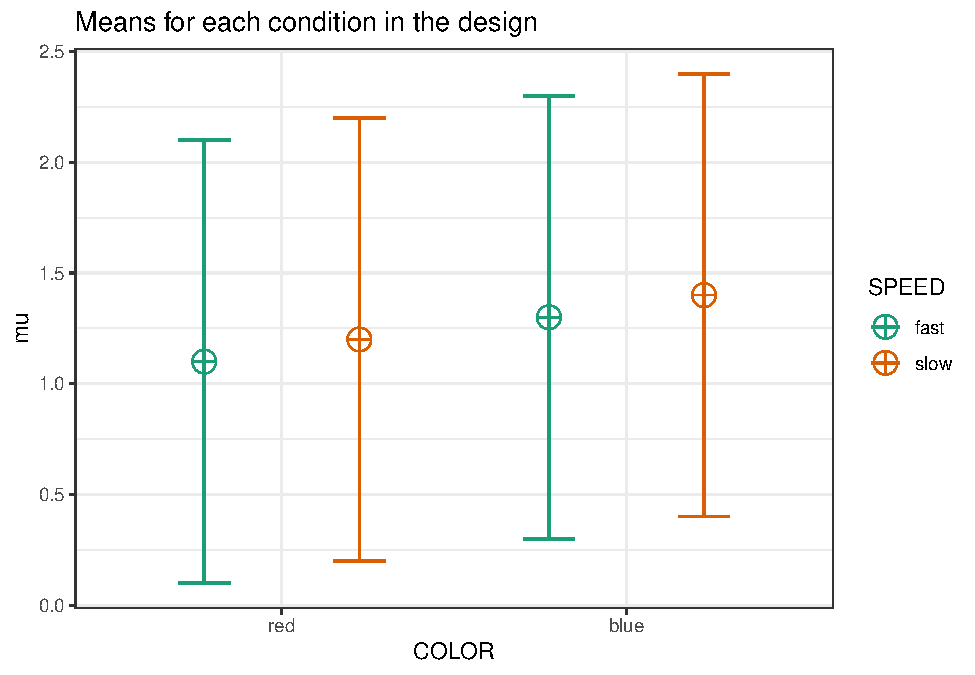
\includegraphics{SuperpowerValidation_files/figure-latex/unnamed-chunk-4-1.pdf}
\newpage
We can check the correlation matrix by asking for it from the design\_result object to check if it was entered the way we wanted:

\begin{Shaded}
\begin{Highlighting}[]
\NormalTok{design_result}\OperatorTok{$}\NormalTok{cor_mat}
\end{Highlighting}
\end{Shaded}

\begin{table}[!h]

\caption{\label{tab:unnamed-chunk-6}Correlation Matrix}
\centering
\begin{tabular}{l|r|r|r|r}
\hline
  & red\_fast & red\_slow & blue\_fast & blue\_slow\\
\hline
red\_fast & 1.00 & 0.91 & 0.92 & 0.93\\
\hline
red\_slow & 0.91 & 1.00 & 0.94 & 0.95\\
\hline
blue\_fast & 0.92 & 0.94 & 1.00 & 0.96\\
\hline
blue\_slow & 0.93 & 0.95 & 0.96 & 1.00\\
\hline
\end{tabular}
\end{table}

We should also check the covariance-variance matrix to ensure the \texttt{ANOVA\_design} function working properly.
The variance should be the diagonal element while the off-diagonal elements should be equal to \texttt{covariance\ =\ correlation*variance} or \(cov_{x,y}=\frac{\sum_{i=1}^{N}(x_{i}-\bar{x})(y_{i}-\bar{y})}{N-1}\).
In this case, it is identical to the correlation matrix because the variance is equal to 1.

\begin{Shaded}
\begin{Highlighting}[]
\NormalTok{design_result}\OperatorTok{$}\NormalTok{sigmatrix}
\end{Highlighting}
\end{Shaded}

\begin{table}[!h]

\caption{\label{tab:unnamed-chunk-8}Covariance-Variance Matrix}
\centering
\begin{tabular}{l|r|r|r|r}
\hline
  & red\_fast & red\_slow & blue\_fast & blue\_slow\\
\hline
red\_fast & 1.00 & 0.91 & 0.92 & 0.93\\
\hline
red\_slow & 0.91 & 1.00 & 0.94 & 0.95\\
\hline
blue\_fast & 0.92 & 0.94 & 1.00 & 0.96\\
\hline
blue\_slow & 0.93 & 0.95 & 0.96 & 1.00\\
\hline
\end{tabular}
\end{table}

\hypertarget{specifying-the-sample-size}{%
\subsection{Specifying the sample size}\label{specifying-the-sample-size}}

You can set the sample size \textbf{per condition} by setting a value for \texttt{n}. The assumption is that you will collect equal sample sizes in all conditions {[}expanding Superpower to allow different sample sizes in each group is a planned future option{]}.

This means for the \texttt{2w*2w} design above there is a total of 80 participants/subjects with a total of 320 observations.

\hypertarget{specifying-the-standard-deviation}{%
\subsection{Specifying the standard deviation}\label{specifying-the-standard-deviation}}

You can set the standard deviation(s) by setting a value of \texttt{sd}. Currently, \texttt{Superpower} allows you to \textbf{violate the assumption of homogeneity of variance}. This will affect the type I error rate if the differences in \texttt{sd} between conditions are extreme. Note that there is always some uncertainty in which values you can expect in the study you are planning. It is therefore useful to perform sensitivity analyses (e.g., running the simulation with the expected standard deviation, but also with more conservative or even worst-case-scenario values).

\hypertarget{one-way-anova}{%
\chapter{One-Way ANOVA}\label{one-way-anova}}

\hypertarget{part-1}{%
\section{Part 1}\label{part-1}}

Using the formula also used by \citet{albers2018power}, we can determine the means that should yield a specified effect sizes (expressed in Cohen's \emph{f}). Eta-squared (identical to partial eta-squared for one-way ANOVA's) has benchmarks of .0099, .0588, and .1379 for small, medium, and large effect sizes \citep{cohen1988spa}. Athough these benchmarks are quite arbitrary, and researchers should only use such benchmarks for power analyses as a last resort, we will demonstrate an a priori power analysis for these values.

\hypertarget{two-conditions}{%
\subsection{Two conditions}\label{two-conditions}}

Imagine we aim to design a study to test the hypothesis that giving people a pet to take care of will increase their life satisfaction. We have a control condition, and a condition where people get a pet, and randomly assign participants to either condition. We can simulate a one-way ANOVA with a specified alpha, sample size, and effect size, on see the statistical power we would have for the ANOVA and the follow-up comparisons. We expect pets to increase life-satisfaction compared to the control condition. Based on work by \citet{pavot1993affective} we believe that we can expect responses on the life-satifaction scale to have a mean of approximately 24 in our population, with a standard deviation of 6.4. We expect having a pet increases life satisfaction with approximately 2.2 scale points for participants who get a pet. 200 participants in total, with 100 participants in each condition. But before we proceed with the data collection, we examine the statistical power our design would have to detect the differences we predict.

\begin{Shaded}
\begin{Highlighting}[]
\NormalTok{string <-}\StringTok{ "2b"}
\NormalTok{n <-}\StringTok{ }\DecValTok{100}
\CommentTok{# We are thinking of running 50 peope in each condition}
\NormalTok{mu <-}\StringTok{ }\KeywordTok{c}\NormalTok{(}\DecValTok{24}\NormalTok{, }\FloatTok{26.2}\NormalTok{)}
\CommentTok{# Enter means in the order that matches the labels below.}
\CommentTok{# In this case, control, cat, dog. }
\NormalTok{sd <-}\StringTok{ }\FloatTok{6.4}
\NormalTok{labelnames <-}\StringTok{ }\KeywordTok{c}\NormalTok{(}\StringTok{"condition"}\NormalTok{, }\StringTok{"control"}\NormalTok{, }\StringTok{"pet"}\NormalTok{) }\CommentTok{#}
\CommentTok{# the label names should be in the order of the means specified above.}
\NormalTok{design_result <-}\StringTok{ }\KeywordTok{ANOVA_design}\NormalTok{(}\DataTypeTok{design =}\NormalTok{ string,}
                   \DataTypeTok{n =}\NormalTok{ n, }
                   \DataTypeTok{mu =}\NormalTok{ mu, }
                   \DataTypeTok{sd =}\NormalTok{ sd, }
                   \DataTypeTok{labelnames =}\NormalTok{ labelnames)}
\NormalTok{alpha_level <-}\StringTok{ }\FloatTok{0.05}
\CommentTok{# You should think carefully about how to justify your alpha level.}
\CommentTok{# We will give some examples later, but for now, use 0.05.}
\end{Highlighting}
\end{Shaded}

\begin{Shaded}
\begin{Highlighting}[]
\NormalTok{simulation_result <-}\StringTok{ }\KeywordTok{ANOVA_power}\NormalTok{(design_result, }
                                 \DataTypeTok{alpha_level =}\NormalTok{ alpha_level, }
                                 \DataTypeTok{nsims =}\NormalTok{ nsims,}
                                 \DataTypeTok{verbose =} \OtherTok{FALSE}\NormalTok{)}
\end{Highlighting}
\end{Shaded}

\begin{table}[!h]

\caption{\label{tab:unnamed-chunk-11}Simulated ANOVA Result}
\centering
\begin{tabular}{l|r|r}
\hline
  & power & effect\_size\\
\hline
anova\_condition & 67.2 & 0.0331418\\
\hline
\end{tabular}
\end{table}

\begin{Shaded}
\begin{Highlighting}[]
\NormalTok{exact_result <-}\StringTok{ }\KeywordTok{ANOVA_exact}\NormalTok{(design_result,}
                            \DataTypeTok{alpha_level =}\NormalTok{ alpha_level,}
                            \DataTypeTok{verbose =} \OtherTok{FALSE}\NormalTok{)}
\end{Highlighting}
\end{Shaded}

\begin{table}[!h]

\caption{\label{tab:unnamed-chunk-13}Exact ANOVA Result}
\centering
\begin{tabular}{l|r|r|r|r}
\hline
  & power & partial\_eta\_squared & cohen\_f & non\_centrality\\
\hline
condition & 67.68572 & 0.0289748 & 0.1727409 & 5.908203\\
\hline
\end{tabular}
\end{table}

The result shows that we have exactly the same power for the ANOVA, as we have for the \emph{t}-test. When there are only two groups, these tests are mathematically identical. In a study with 100 participants, we would have quite low power (around 67.7\%). An ANOVA with 2 groups is identical to a \emph{t}-test. For our example, Cohen's d (the standardized mean difference) is 2.2/6.4, or d = 0.34375 for the difference between the control condition and pets, which we can use to easily compute the expected power for these simple comparisons using the \texttt{pwr} \citeyearpar{R-pwr} package.

\begin{Shaded}
\begin{Highlighting}[]
\KeywordTok{pwr.t.test}\NormalTok{(}\DataTypeTok{d =} \FloatTok{2.2}\OperatorTok{/}\FloatTok{6.4}\NormalTok{,}
           \DataTypeTok{n =} \DecValTok{100}\NormalTok{,}
           \DataTypeTok{sig.level =} \FloatTok{0.05}\NormalTok{,}
           \DataTypeTok{type =} \StringTok{"two.sample"}\NormalTok{,}
           \DataTypeTok{alternative =} \StringTok{"two.sided"}\NormalTok{)}\OperatorTok{$}\NormalTok{power}
\end{Highlighting}
\end{Shaded}

\begin{verbatim}
## [1] 0.6768572
\end{verbatim}

We can also directly compute Cohen's \emph{f} from Cohen's d for two groups, as \citet{cohen1988spa} describes, because \emph{f} = 1/2d. So \emph{f} = 0.5*0.34375 = 0.171875. And indeed, power analysis using the pwr package yields the same result using the \texttt{pwr.anova.test} as the \texttt{power.t.test}.

\begin{Shaded}
\begin{Highlighting}[]
\NormalTok{K <-}\StringTok{ }\DecValTok{2}
\NormalTok{n <-}\StringTok{ }\DecValTok{100}
\NormalTok{f <-}\StringTok{ }\FloatTok{0.171875}
\KeywordTok{pwr.anova.test}\NormalTok{(}\DataTypeTok{n =}\NormalTok{ n,}
               \DataTypeTok{k =}\NormalTok{ K,}
               \DataTypeTok{f =}\NormalTok{ f,}
               \DataTypeTok{sig.level =}\NormalTok{ alpha_level)}\OperatorTok{$}\NormalTok{power}
\end{Highlighting}
\end{Shaded}

\begin{verbatim}
## [1] 0.6768572
\end{verbatim}

This analysis tells us that running the study with 100 participants in each condition is too likely to \emph{not} yield a significant test result, even if our expected pattern of differences is true. This is not optimal.

Let's mathematically explore which pattern of means we would need to expect to habe 90\% power for the ANOVA with 50 participants in each group. We can use the pwr package in R to compute a sensitivity analysis that tells us the effect size, in Cohen's \emph{f}, that we are able to detect with 3 groups and 50 partiicpants in each group, in order to achive 90\% power with an alpha level of 5\%.

\begin{Shaded}
\begin{Highlighting}[]
\NormalTok{K <-}\StringTok{ }\DecValTok{2}
\NormalTok{n <-}\StringTok{ }\DecValTok{100}
\NormalTok{sd <-}\StringTok{ }\FloatTok{6.4}
\NormalTok{r <-}\StringTok{ }\DecValTok{0}
\CommentTok{#Calculate f when running simulation}
\NormalTok{f <-}\StringTok{ }\KeywordTok{pwr.anova.test}\NormalTok{(}\DataTypeTok{n =}\NormalTok{ n,}
                    \DataTypeTok{k =}\NormalTok{ K,}
                    \DataTypeTok{power =} \FloatTok{0.9}\NormalTok{,}
                    \DataTypeTok{sig.level =}\NormalTok{ alpha_level)}\OperatorTok{$}\NormalTok{f}
\NormalTok{f}
\end{Highlighting}
\end{Shaded}

\begin{verbatim}
## [1] 0.2303587
\end{verbatim}

This sensitivity analysis shows we have 90\% power in our planned design to detect effects of Cohen's \emph{f} of 0.2303587. Benchmarks by \citet{cohen1988spa} for small, medium, and large Cohen's \emph{f} values are 0.1, 0.25, and 0.4, which correspond to eta-squared values of small (.0099), medium (.0588), and large (.1379), in line with d = .2, .5, or .8. So, at least based on these benchmarks, we have 90\% power to detect effects that are slightly below a medium effect benchmark.

\begin{Shaded}
\begin{Highlighting}[]
\NormalTok{f2 <-}\StringTok{ }\NormalTok{f}\OperatorTok{^}\DecValTok{2}
\NormalTok{ES <-}\StringTok{ }\NormalTok{f2 }\OperatorTok{/}\StringTok{ }\NormalTok{(f2 }\OperatorTok{+}\StringTok{ }\DecValTok{1}\NormalTok{)}
\NormalTok{ES}
\end{Highlighting}
\end{Shaded}

\begin{verbatim}
## [1] 0.0503911
\end{verbatim}

Expressed in eta-squared, we can detect values of eta-squared = 0.05 or larger.

\begin{Shaded}
\begin{Highlighting}[]
\NormalTok{mu <-}\StringTok{ }\KeywordTok{mu_from_ES}\NormalTok{(}\DataTypeTok{K =}\NormalTok{ K, }\DataTypeTok{ES =}\NormalTok{ ES)}
\NormalTok{mu <-}\StringTok{ }\NormalTok{mu }\OperatorTok{*}\StringTok{ }\NormalTok{sd}
\NormalTok{mu}
\end{Highlighting}
\end{Shaded}

\begin{verbatim}
## [1] -1.474295  1.474295
\end{verbatim}

We can compute a pattern of means, given a standard deviation of 6.4, that would give us an effect size of \emph{f} = 0.23, or eta-squared of 0.05. We should be able to accomplish this is the means are -1.474295 and 1.474295. We can use these values to confirm the ANOVA has 90\% power.

\begin{Shaded}
\begin{Highlighting}[]
\NormalTok{design_result <-}\StringTok{ }\KeywordTok{ANOVA_design}\NormalTok{(}
  \DataTypeTok{design =}\NormalTok{ string,}
  \DataTypeTok{n =}\NormalTok{ n,}
  \DataTypeTok{mu =}\NormalTok{ mu,}
  \DataTypeTok{sd =}\NormalTok{ sd,}
  \DataTypeTok{labelnames =}\NormalTok{ labelnames}
\NormalTok{  )}
\end{Highlighting}
\end{Shaded}

\begin{Shaded}
\begin{Highlighting}[]
\NormalTok{simulation_result <-}\StringTok{ }\KeywordTok{ANOVA_power}\NormalTok{(design_result, }
                                 \DataTypeTok{alpha_level =}\NormalTok{ alpha_level, }
                                 \DataTypeTok{nsims =}\NormalTok{ nsims,}
                                 \DataTypeTok{verbose =} \OtherTok{FALSE}\NormalTok{)}
\end{Highlighting}
\end{Shaded}

\begin{table}[!h]

\caption{\label{tab:unnamed-chunk-21}Simulated ANOVA Result}
\centering
\begin{tabular}{l|r|r}
\hline
  & power & effect\_size\\
\hline
anova\_condition & 90.15 & 0.0544974\\
\hline
\end{tabular}
\end{table}

\begin{Shaded}
\begin{Highlighting}[]
\NormalTok{exact_result <-}\StringTok{ }\KeywordTok{ANOVA_exact}\NormalTok{(design_result,}
                            \DataTypeTok{alpha_level =}\NormalTok{ alpha_level,}
                            \DataTypeTok{verbose =} \OtherTok{FALSE}\NormalTok{)}
\end{Highlighting}
\end{Shaded}

\begin{table}[!h]

\caption{\label{tab:unnamed-chunk-23}Exact ANOVA Result}
\centering
\begin{tabular}{l|r|r|r|r}
\hline
  & power & partial\_eta\_squared & cohen\_f & non\_centrality\\
\hline
condition & 90.00714 & 0.0508742 & 0.2315192 & 10.61302\\
\hline
\end{tabular}
\end{table}

The simulation confirms that for the \emph{F}-test for the ANOVA we have 90\% power. This is also what Gpower tells us what would happen based on a post-hoc power analysis with an \emph{f} of 0.2303587, 2 groups, 200 participants in total (100 in each between subject condition), and an alpha of 5\%.

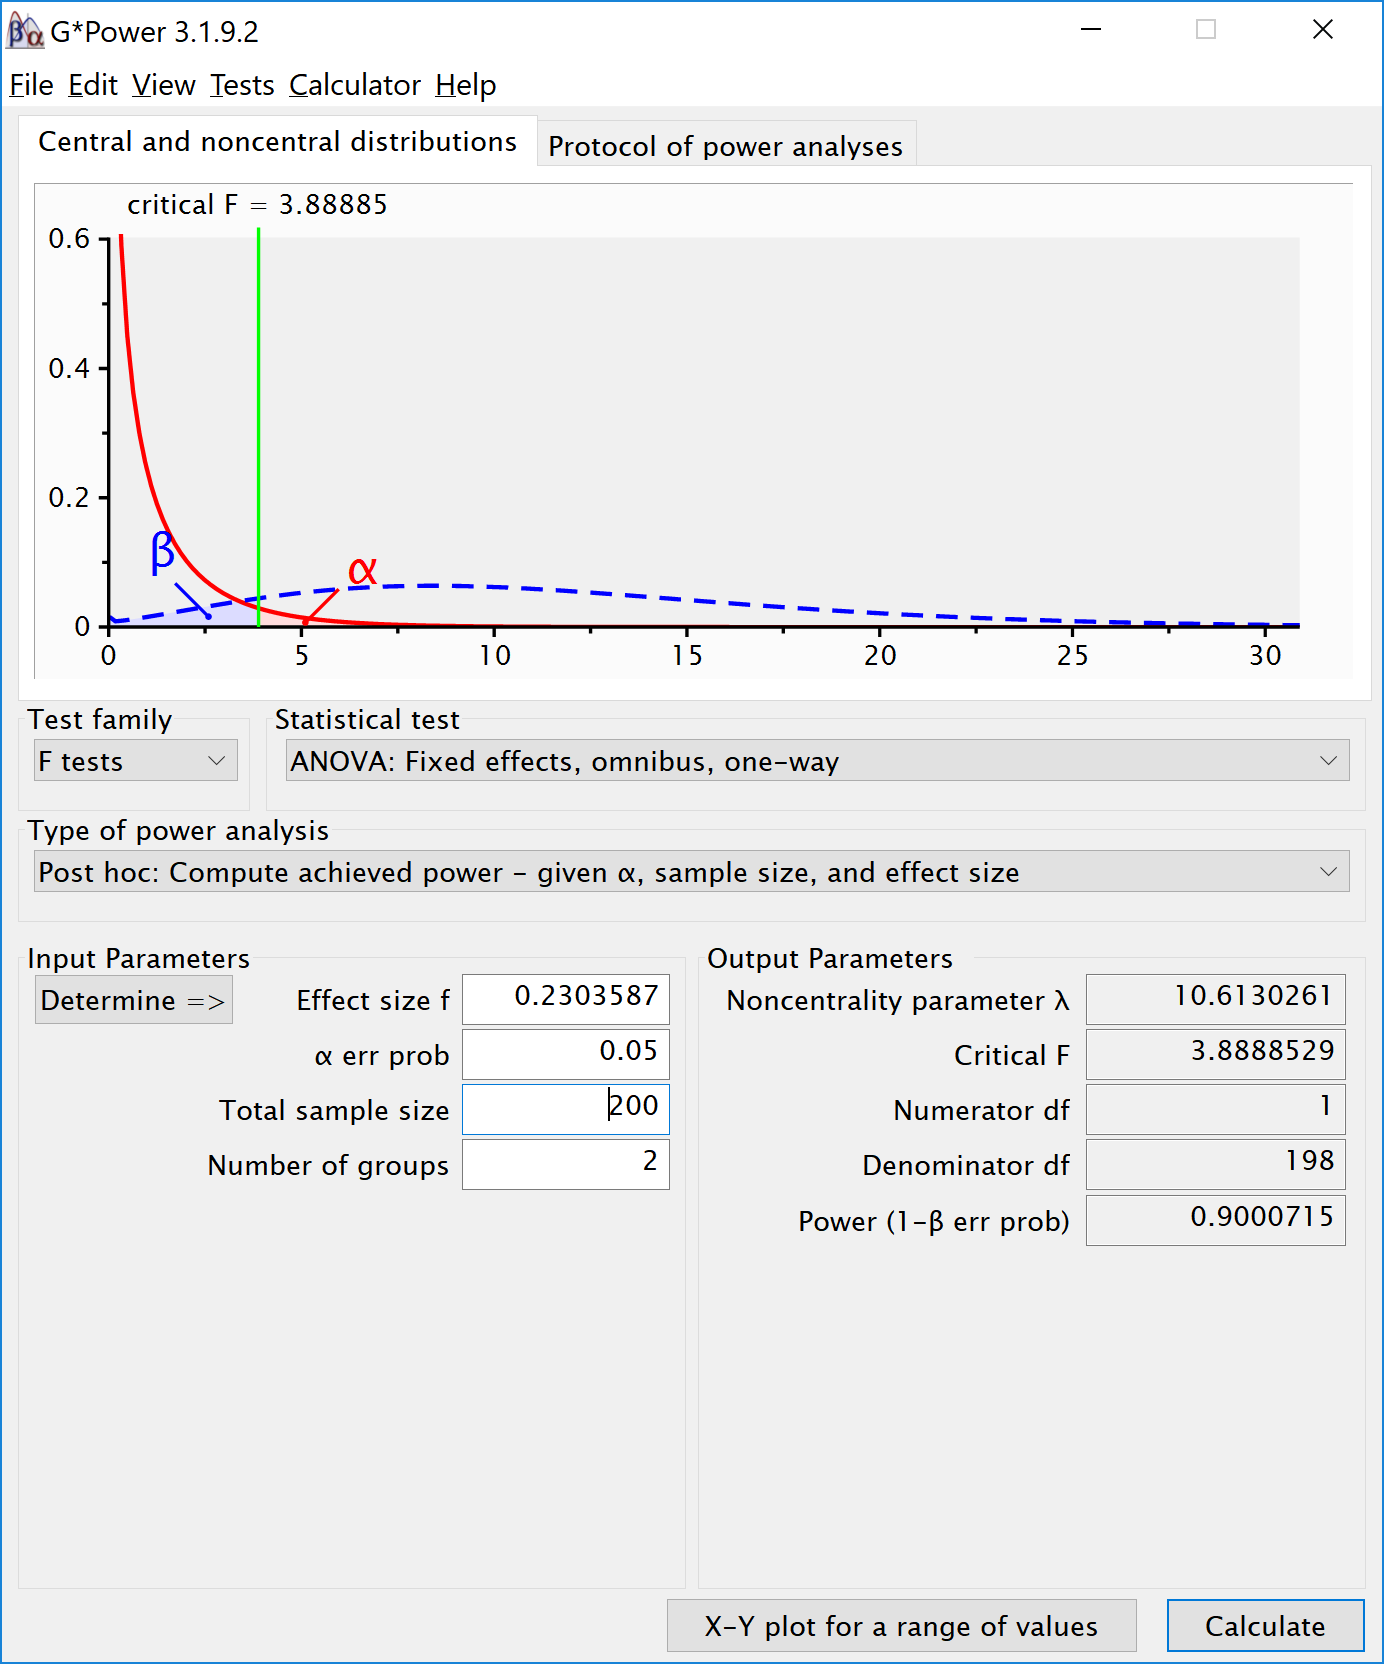
\includegraphics{screenshots/gpower_8.png}

If we return to our expected means, how many participants do we need for sufficient power? Given the expected difference and standard deviation, d = 0.34375, and \emph{f} = 0.171875. We can perform an a priori power analysis for this simple case, which tells us we need 179 participants in each group (we can't split people in parts, and thus always round a power analysis upward), or 358 in total.

\begin{Shaded}
\begin{Highlighting}[]
\NormalTok{K <-}\StringTok{ }\DecValTok{2}
\NormalTok{power <-}\StringTok{ }\FloatTok{0.9}
\NormalTok{f <-}\StringTok{ }\FloatTok{0.171875}
\KeywordTok{pwr.anova.test}\NormalTok{(}\DataTypeTok{power =}\NormalTok{ power,}
               \DataTypeTok{k =}\NormalTok{ K,}
               \DataTypeTok{f =}\NormalTok{ f,}
               \DataTypeTok{sig.level =}\NormalTok{ alpha_level)}
\end{Highlighting}
\end{Shaded}

\begin{verbatim}
## 
##      Balanced one-way analysis of variance power calculation 
## 
##               k = 2
##               n = 178.8104
##               f = 0.171875
##       sig.level = 0.05
##           power = 0.9
## 
## NOTE: n is number in each group
\end{verbatim}

If we re-run the simulation with this sample size, we indeed have 90\% power.

\begin{Shaded}
\begin{Highlighting}[]
\NormalTok{string <-}\StringTok{ "2b"}
\NormalTok{n <-}\StringTok{ }\DecValTok{179}
\NormalTok{mu <-}\StringTok{ }\KeywordTok{c}\NormalTok{(}\DecValTok{24}\NormalTok{, }\FloatTok{26.2}\NormalTok{)}
\CommentTok{# Enter means in the order that matches the labels below.}
\CommentTok{# In this case, control, pet.}
\NormalTok{sd <-}\StringTok{ }\FloatTok{6.4}
\NormalTok{labelnames <-}\StringTok{ }\KeywordTok{c}\NormalTok{(}\StringTok{"condition"}\NormalTok{, }\StringTok{"control"}\NormalTok{, }\StringTok{"pet"}\NormalTok{) }\CommentTok{#}
\CommentTok{# the label names should be in the order of the means specified above.}
\NormalTok{design_result <-}\StringTok{ }\KeywordTok{ANOVA_design}\NormalTok{(}
\DataTypeTok{design =}\NormalTok{ string,}
\DataTypeTok{n =}\NormalTok{ n,}
\DataTypeTok{mu =}\NormalTok{ mu,}
\DataTypeTok{sd =}\NormalTok{ sd,}
\DataTypeTok{labelnames =}\NormalTok{ labelnames}
\NormalTok{)}
\NormalTok{alpha_level <-}\StringTok{ }\FloatTok{0.05}
\end{Highlighting}
\end{Shaded}

\begin{Shaded}
\begin{Highlighting}[]
\NormalTok{simulation_result <-}\StringTok{ }\KeywordTok{ANOVA_power}\NormalTok{(design_result, }
                                 \DataTypeTok{alpha_level =}\NormalTok{ alpha_level, }
                                 \DataTypeTok{nsims =}\NormalTok{ nsims,}
                                 \DataTypeTok{verbose =} \OtherTok{FALSE}\NormalTok{)}
\end{Highlighting}
\end{Shaded}

\begin{table}[!h]

\caption{\label{tab:unnamed-chunk-27}Simulated ANOVA Result}
\centering
\begin{tabular}{l|r|r}
\hline
  & power & effect\_size\\
\hline
anova\_condition & 89.99 & 0.0315708\\
\hline
\end{tabular}
\end{table}

\begin{Shaded}
\begin{Highlighting}[]
\NormalTok{exact_result <-}\StringTok{ }\KeywordTok{ANOVA_exact}\NormalTok{(design_result,}
                            \DataTypeTok{alpha_level =}\NormalTok{ alpha_level,}
                            \DataTypeTok{verbose =} \OtherTok{FALSE}\NormalTok{)}
\end{Highlighting}
\end{Shaded}

\begin{table}[!h]

\caption{\label{tab:unnamed-chunk-29}Exact ANOVA Result}
\centering
\begin{tabular}{l|r|r|r|r}
\hline
  & power & partial\_eta\_squared & cohen\_f & non\_centrality\\
\hline
condition & 90.03028 & 0.0288499 & 0.1723571 & 10.57568\\
\hline
\end{tabular}
\end{table}

We stored the result from the power analysis in an object. This allows us to request plots (which are not printed automatically) showing the \emph{p}-value distribution. If we request \texttt{simulation\_result\$plot1} we get the p-value distribution for the ANOVA:

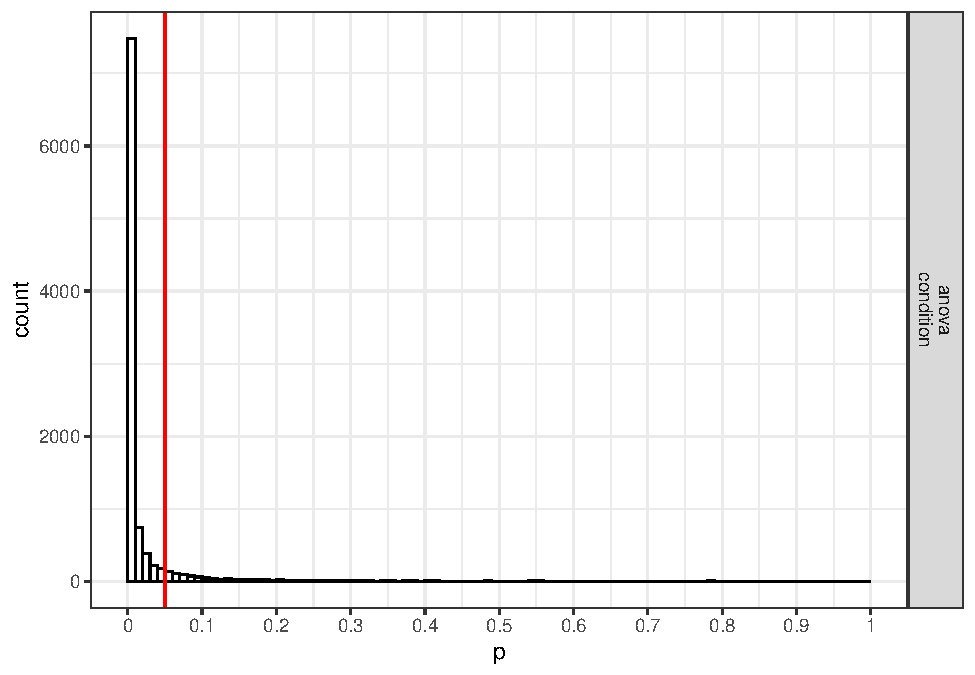
\includegraphics{SuperpowerValidation_files/figure-latex/unnamed-chunk-30-1.pdf}

If we request \texttt{simulation\_result\$plot2} we get the p-value distribution for the paired comparisons (in this case only one):

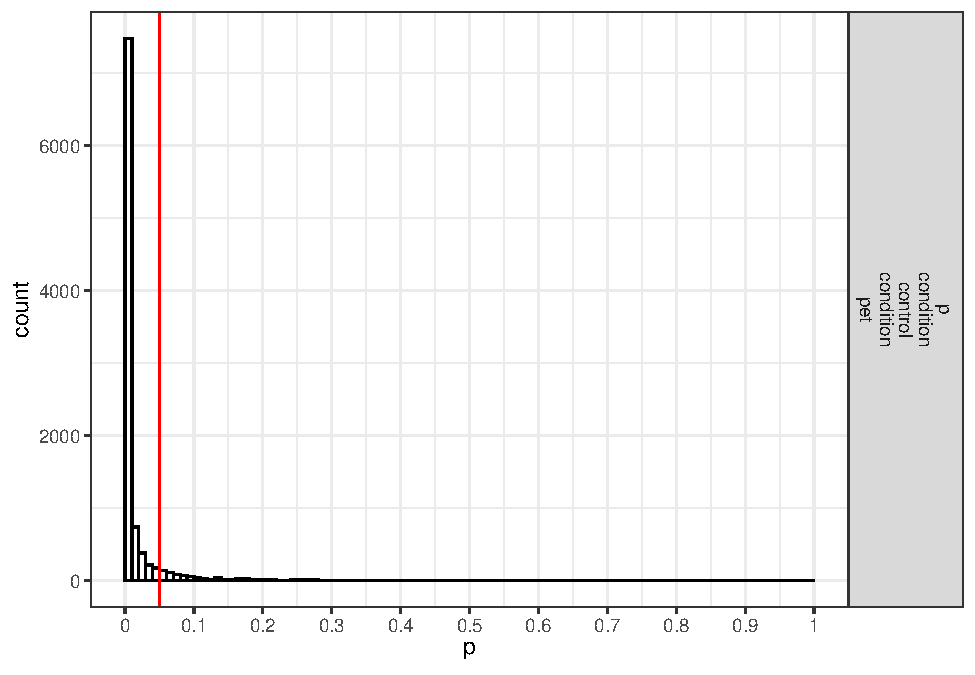
\includegraphics{SuperpowerValidation_files/figure-latex/unnamed-chunk-31-1.pdf}
\newpage
\#\# Part 2

\hypertarget{three-conditions}{%
\subsection{Three conditions}\label{three-conditions}}

Imagine we aim to design a study to test the hypothesis that giving people a pet to take care of will increase their life satisfaction. We have a control condition, a `cat' pet condition, and a `dog' pet condition. We can simulate a One-Way ANOVA with a specified alpha, sample size, and effect size, on see the statistical power we would have for the ANOVA and the follow-up comparisons. We expect all pets to increase life-satisfaction compared to the control condition. Obviously, we also expect the people who are in the `dog' pet condition to have even greater life-satisfaction than people in the `cat' pet condition. Based on work by Pavot and Diener (1993) we believe that we can expect responses on the life-satifaction scale to have a mean of approximately 24 in our population, with a standard deviation of 6.4. We expect having a pet increases life satisfaction with approximately 2.2 scale points for participants who get a cat, and 2.6 scale points for participants who get a dog. We initially consider collecting data from 150 participants in total, with 50 participants in each condition. But before we proceed with the data collection, we examine the statistical power our design would have to detect the differences we predict.

\begin{Shaded}
\begin{Highlighting}[]
\NormalTok{string <-}\StringTok{ "3b"}
\NormalTok{n <-}\StringTok{ }\DecValTok{50}
\CommentTok{# We are thinking of running 50 peope in each condition}
\NormalTok{mu <-}\StringTok{ }\KeywordTok{c}\NormalTok{(}\DecValTok{24}\NormalTok{, }\FloatTok{26.2}\NormalTok{, }\FloatTok{26.6}\NormalTok{)}
\CommentTok{# Enter means in the order that matches the labels below.}
\CommentTok{# In this case, control, cat, dog.}
\NormalTok{sd <-}\StringTok{ }\FloatTok{6.4}
\NormalTok{labelnames <-}\StringTok{ }\KeywordTok{c}\NormalTok{(}\StringTok{"condition"}\NormalTok{, }\StringTok{"control"}\NormalTok{, }\StringTok{"cat"}\NormalTok{, }\StringTok{"dog"}\NormalTok{) }\CommentTok{#}
\CommentTok{# the label names should be in the order of the means specified above.}
\NormalTok{design_result <-}\StringTok{ }\KeywordTok{ANOVA_design}\NormalTok{(}
\DataTypeTok{design =}\NormalTok{ string,}
\DataTypeTok{n =}\NormalTok{ n,}
\DataTypeTok{mu =}\NormalTok{ mu,}
\DataTypeTok{sd =}\NormalTok{ sd,}
\DataTypeTok{labelnames =}\NormalTok{ labelnames}
\NormalTok{)}
\NormalTok{alpha_level <-}\StringTok{ }\FloatTok{0.05}
\end{Highlighting}
\end{Shaded}

\begin{Shaded}
\begin{Highlighting}[]
\CommentTok{# You should think carefully about how to justify your alpha level.}
\CommentTok{# We will give some examples later, but for now, use 0.05.}
\NormalTok{simulation_result <-}\StringTok{ }\KeywordTok{ANOVA_power}\NormalTok{(design_result, }
                                 \DataTypeTok{alpha_level =}\NormalTok{ alpha_level, }
                                 \DataTypeTok{nsims =}\NormalTok{ nsims,}
                                 \DataTypeTok{verbose =} \OtherTok{FALSE}\NormalTok{)}
\end{Highlighting}
\end{Shaded}

\begin{table}[!h]

\caption{\label{tab:unnamed-chunk-34}Simulated ANOVA Result}
\centering
\begin{tabular}{l|r|r}
\hline
  & power & effect\_size\\
\hline
anova\_condition & 47.26 & 0.0433997\\
\hline
\end{tabular}
\end{table}

\begin{Shaded}
\begin{Highlighting}[]
\NormalTok{exact_result <-}\StringTok{ }\KeywordTok{ANOVA_exact}\NormalTok{(design_result,}
                            \DataTypeTok{alpha_level =}\NormalTok{ alpha_level,}
                            \DataTypeTok{verbose =} \OtherTok{FALSE}\NormalTok{)}
\end{Highlighting}
\end{Shaded}

\begin{table}[!h]

\caption{\label{tab:unnamed-chunk-36}Exact ANOVA Result}
\centering
\begin{tabular}{l|r|r|r|r}
\hline
  & power & partial\_eta\_squared & cohen\_f & non\_centrality\\
\hline
condition & 47.69468 & 0.0315259 & 0.180422 & 4.785156\\
\hline
\end{tabular}
\end{table}

The result shows that you would have quite low power with 50 participants, both for the overall ANOVA (just around 50\% power), as for the follow up comparisons (approximately 40\% power for the control vs cat condition, around 50\% for the control vs dogs condition, and a really low power (around 6\%, just above the Type 1 error rate of 5\%) for the expected difference between cats and dogs.

\hypertarget{power-for-simple-effects}{%
\subsection{Power for simple effects}\label{power-for-simple-effects}}

We are typically not just interested in the ANOVA, but also in follow up comparisons. In this case, we would perform a \emph{t}-test comparing the control condition against the cat and dog condition, and we would compare the cat and dog conditions against each other, in independent \emph{t}-tests.

For our example, Cohen's d (the standardized mean difference) is 2.2/6.4, or d = 0.34375 for the difference between the control condition and cats, 2.6/6.4 of d = 0.40625 for the difference between the control condition and dogs, and 0.4/6.4 or d = 0.0625 for the difference between cats and dogs as pets.

We can easily compute the expected power for these simple comparisons using the pwr package.

\begin{Shaded}
\begin{Highlighting}[]
\KeywordTok{pwr.t.test}\NormalTok{(}
  \DataTypeTok{d =} \FloatTok{2.2} \OperatorTok{/}\StringTok{ }\FloatTok{6.4}\NormalTok{,}
  \DataTypeTok{n =} \DecValTok{50}\NormalTok{,}
  \DataTypeTok{sig.level =} \FloatTok{0.05}\NormalTok{,}
  \DataTypeTok{type =} \StringTok{"two.sample"}\NormalTok{,}
  \DataTypeTok{alternative =} \StringTok{"two.sided"}
\NormalTok{  )}\OperatorTok{$}\NormalTok{power}
\end{Highlighting}
\end{Shaded}

\begin{verbatim}
## [1] 0.3983064
\end{verbatim}

\begin{Shaded}
\begin{Highlighting}[]
  \KeywordTok{pwr.t.test}\NormalTok{(}
  \DataTypeTok{d =} \FloatTok{2.6} \OperatorTok{/}\StringTok{ }\FloatTok{6.4}\NormalTok{,}
  \DataTypeTok{n =} \DecValTok{50}\NormalTok{,}
  \DataTypeTok{sig.level =} \FloatTok{0.05}\NormalTok{,}
  \DataTypeTok{type =} \StringTok{"two.sample"}\NormalTok{,}
  \DataTypeTok{alternative =} \StringTok{"two.sided"}
\NormalTok{  )}\OperatorTok{$}\NormalTok{power}
\end{Highlighting}
\end{Shaded}

\begin{verbatim}
## [1] 0.5205162
\end{verbatim}

\begin{Shaded}
\begin{Highlighting}[]
  \KeywordTok{pwr.t.test}\NormalTok{(}
  \DataTypeTok{d =} \FloatTok{0.4} \OperatorTok{/}\StringTok{ }\FloatTok{6.4}\NormalTok{,}
  \DataTypeTok{n =} \DecValTok{50}\NormalTok{,}
  \DataTypeTok{sig.level =} \FloatTok{0.05}\NormalTok{,}
  \DataTypeTok{type =} \StringTok{"two.sample"}\NormalTok{,}
  \DataTypeTok{alternative =} \StringTok{"two.sided"}
\NormalTok{  )}\OperatorTok{$}\NormalTok{power}
\end{Highlighting}
\end{Shaded}

\begin{verbatim}
## [1] 0.06104044
\end{verbatim}

This analysis tells us that running the study with 50 participants in each condition is more likely to \emph{not} yield a significant test result, even if our expected pattern of differences is true, than that we will observe a \emph{p}-value smaller than our alpha level. This is not optimal.

Let's mathematically explore which pattern of means we would need to expect to habe 90\% power for the ANOVA with 50 participants in each group. We can use the pwr package in R to compute a sensitivity analysis that tells us the effect size, in Cohen's \emph{f}, that we are able to detect with 3 groups and 50 partiicpants in each group, in order to achive 90\% power with an alpha level of 5\%.

\begin{Shaded}
\begin{Highlighting}[]
\NormalTok{K <-}\StringTok{ }\DecValTok{3}
\NormalTok{n <-}\StringTok{ }\DecValTok{50}
\NormalTok{sd <-}\StringTok{ }\FloatTok{6.4}
\NormalTok{r <-}\StringTok{ }\DecValTok{0}
\CommentTok{#Calculate f when running simulation}
\NormalTok{f <-}\StringTok{ }\KeywordTok{pwr.anova.test}\NormalTok{(}\DataTypeTok{n =}\NormalTok{ n,}
                    \DataTypeTok{k =}\NormalTok{ K,}
                    \DataTypeTok{power =} \FloatTok{0.9}\NormalTok{,}
                    \DataTypeTok{sig.level =}\NormalTok{ alpha_level)}\OperatorTok{$}\NormalTok{f}
\NormalTok{f}
\end{Highlighting}
\end{Shaded}

\begin{verbatim}
## [1] 0.2934417
\end{verbatim}

This sensitivity analysis shows we have 90\% power in our planned design to detect effects of Cohen's \emph{f} of 0.2934417. Benchmarks by \citet{cohen1988spa} for small, medium, and large Cohen's \emph{f} values are 0.1, 0.25, and 0.4, which correspond to eta-squared values of small (.0099), medium (.0588), and large (.1379), in line with d = .2, .5, or .8. So, at least based on these benchmarks, we have 90\% power to detect effects that are somewhat sizeable.

\begin{Shaded}
\begin{Highlighting}[]
\NormalTok{f2 <-}\StringTok{ }\NormalTok{f}\OperatorTok{^}\DecValTok{2}
\NormalTok{ES <-}\StringTok{ }\NormalTok{f2 }\OperatorTok{/}\StringTok{ }\NormalTok{(f2 }\OperatorTok{+}\StringTok{ }\DecValTok{1}\NormalTok{)}
\NormalTok{ES}
\end{Highlighting}
\end{Shaded}

\begin{verbatim}
## [1] 0.07928127
\end{verbatim}

Expressed in eta-squared, we can detect values of eta-squared = 0.0793 or larger.

\begin{Shaded}
\begin{Highlighting}[]
\NormalTok{mu <-}\StringTok{ }\KeywordTok{mu_from_ES}\NormalTok{(}\DataTypeTok{K =}\NormalTok{ K, }\DataTypeTok{ES =}\NormalTok{ ES)}
\NormalTok{mu <-}\StringTok{ }\NormalTok{mu }\OperatorTok{*}\StringTok{ }\NormalTok{sd}
\NormalTok{mu}
\end{Highlighting}
\end{Shaded}

\begin{verbatim}
## [1] -2.300104  0.000000  2.300104
\end{verbatim}

We can compute a pattern of means, given a standard deviation of 6.4, that would give us an effect size of f = 0.2934, or eta-squared of 0.0793. We should be able to accomplish this is the means are -2.300104, 0.000000, and 2.300104. We can use these values to confirm the ANOVA has 90\% power.

\begin{Shaded}
\begin{Highlighting}[]
\NormalTok{design_result <-}\StringTok{ }\KeywordTok{ANOVA_design}\NormalTok{(}
  \DataTypeTok{design =}\NormalTok{ string,}
  \DataTypeTok{n =}\NormalTok{ n,}
  \DataTypeTok{mu =}\NormalTok{ mu,}
  \DataTypeTok{sd =}\NormalTok{ sd,}
  \DataTypeTok{labelnames =}\NormalTok{ labelnames}
\NormalTok{  )}
\end{Highlighting}
\end{Shaded}

\begin{Shaded}
\begin{Highlighting}[]
\NormalTok{simulation_result <-}\StringTok{ }\KeywordTok{ANOVA_power}\NormalTok{(design_result, }
                                 \DataTypeTok{alpha_level =}\NormalTok{ alpha_level, }
                                 \DataTypeTok{nsims =}\NormalTok{ nsims,}
                                 \DataTypeTok{verbose =} \OtherTok{FALSE}\NormalTok{)}
\end{Highlighting}
\end{Shaded}

\begin{table}[!h]

\caption{\label{tab:unnamed-chunk-43}Simulated ANOVA Result}
\centering
\begin{tabular}{l|r|r}
\hline
  & power & effect\_size\\
\hline
anova\_condition & 90.3 & 0.090741\\
\hline
\end{tabular}
\end{table}

\begin{Shaded}
\begin{Highlighting}[]
\NormalTok{exact_result <-}\StringTok{ }\KeywordTok{ANOVA_exact}\NormalTok{(design_result,}
                            \DataTypeTok{alpha_level =}\NormalTok{ alpha_level,}
                            \DataTypeTok{verbose =} \OtherTok{FALSE}\NormalTok{)}
\end{Highlighting}
\end{Shaded}

\begin{table}[!h]

\caption{\label{tab:unnamed-chunk-45}Exact ANOVA Result}
\centering
\begin{tabular}{l|r|r|r|r}
\hline
  & power & partial\_eta\_squared & cohen\_f & non\_centrality\\
\hline
condition & 90.00112 & 0.0807686 & 0.2964209 & 12.9162\\
\hline
\end{tabular}
\end{table}

The simulation confirms that for the \emph{F}-test for the ANOVA we have 90\% power. This is also what g*power tells us what would happen based on a post-hoc power analysis with an f of 0.2934417, 3 groups, 150 participants in total (50 in each between subject condition), and an alpha of 5\%.

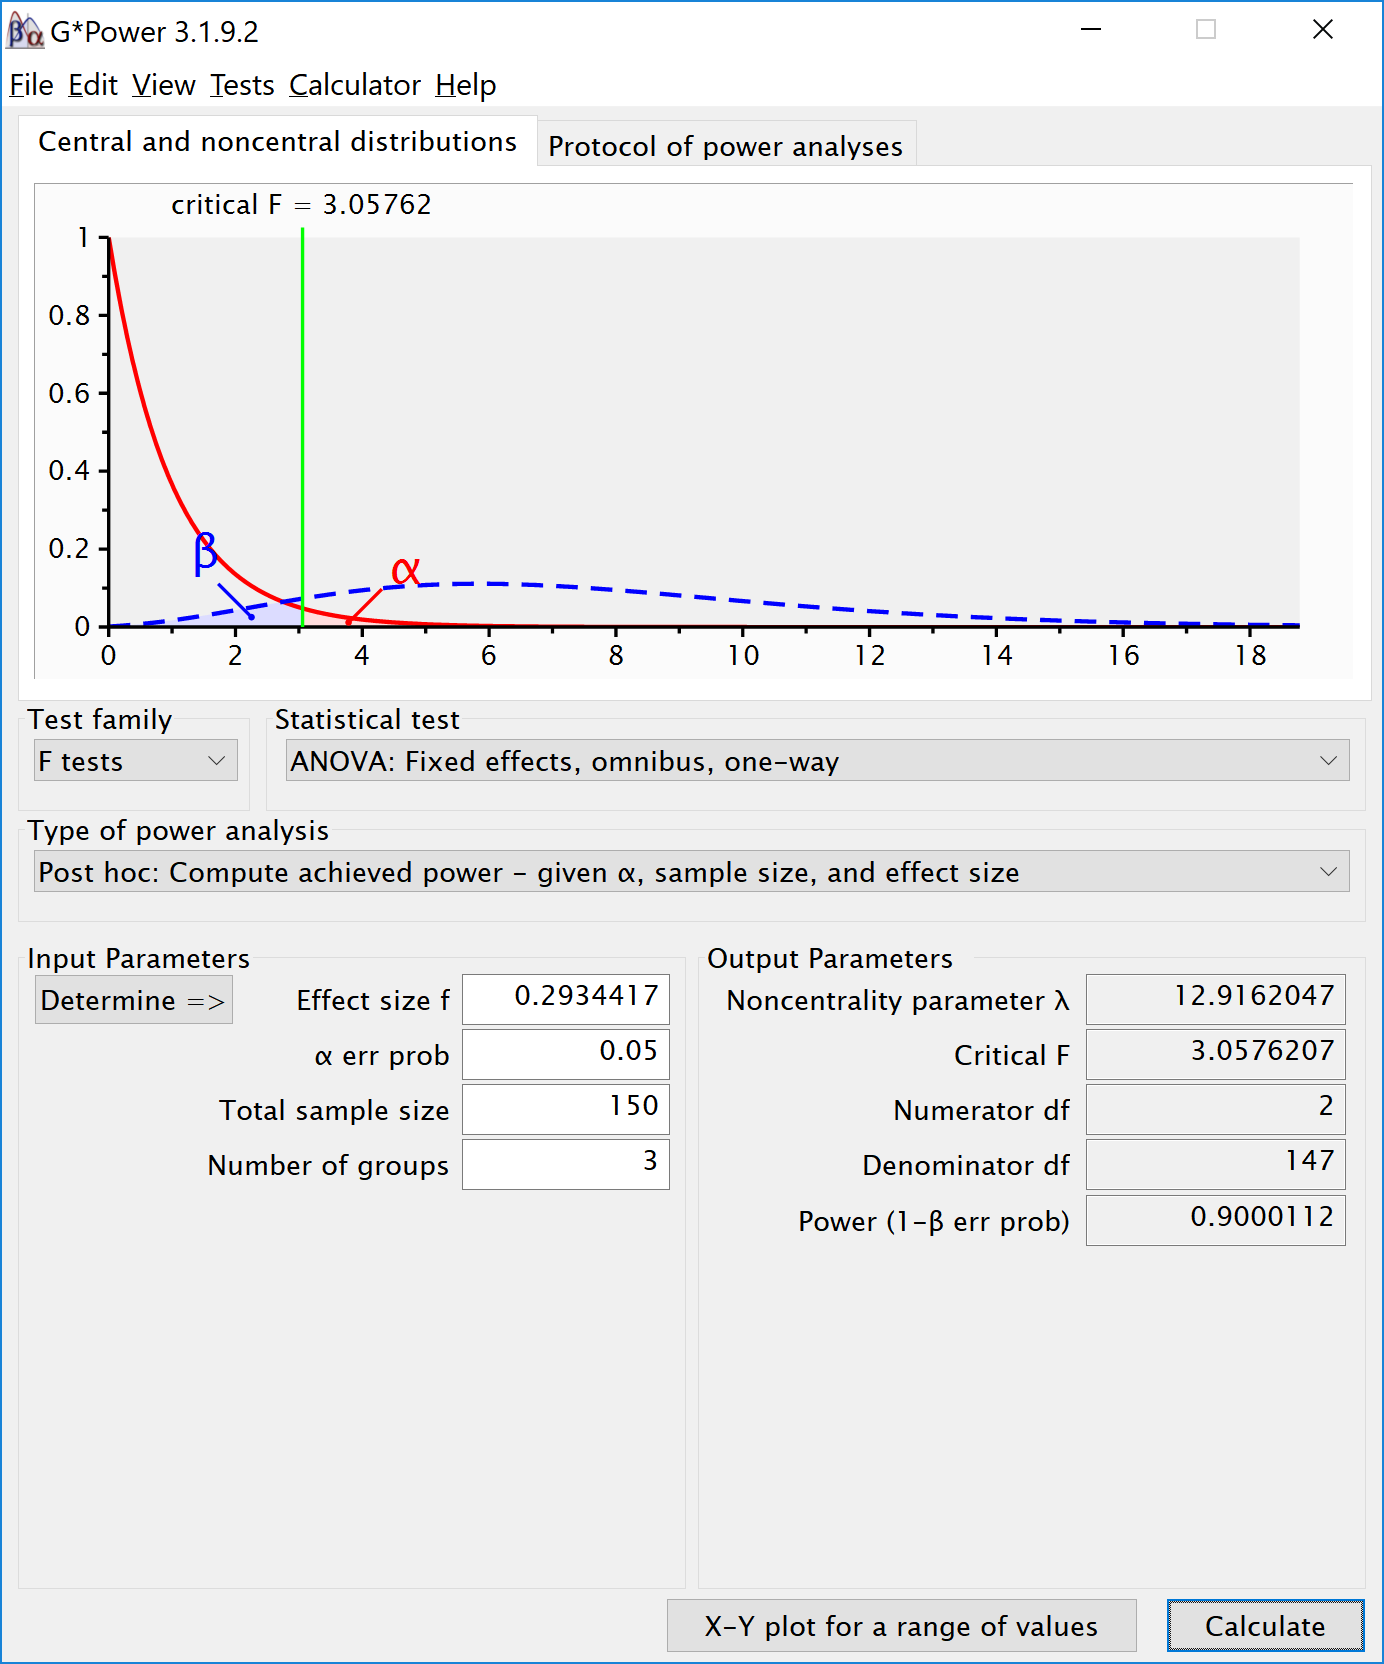
\includegraphics{screenshots/gpower_7.png}

We can also compute the power for the ANOVA and simple effects in \texttt{R} with the \texttt{pwr} package. The calculated effect sizes and power match those from the simulation.

\begin{Shaded}
\begin{Highlighting}[]
\NormalTok{K <-}\StringTok{ }\DecValTok{3}
\NormalTok{n <-}\StringTok{ }\DecValTok{50}
\NormalTok{sd <-}\StringTok{ }\FloatTok{6.4}
\NormalTok{f <-}\StringTok{ }\FloatTok{0.2934417}
\KeywordTok{pwr.anova.test}\NormalTok{(}
\DataTypeTok{n =}\NormalTok{ n,}
\DataTypeTok{k =}\NormalTok{ K,}
\DataTypeTok{f =}\NormalTok{ f,}
\DataTypeTok{sig.level =}\NormalTok{ alpha_level}
\NormalTok{)}\OperatorTok{$}\NormalTok{power}
\end{Highlighting}
\end{Shaded}

\begin{verbatim}
## [1] 0.9000112
\end{verbatim}

\begin{Shaded}
\begin{Highlighting}[]
\NormalTok{d <-}\StringTok{ }\FloatTok{2.300104} \OperatorTok{/}\StringTok{ }\FloatTok{6.4}
\NormalTok{d}
\end{Highlighting}
\end{Shaded}

\begin{verbatim}
## [1] 0.3593912
\end{verbatim}

\begin{Shaded}
\begin{Highlighting}[]
\KeywordTok{pwr.t.test}\NormalTok{(}
\DataTypeTok{d =} \FloatTok{2.300104} \OperatorTok{/}\StringTok{ }\FloatTok{6.4}\NormalTok{,}
\DataTypeTok{n =} \DecValTok{50}\NormalTok{,}
\DataTypeTok{sig.level =} \FloatTok{0.05}\NormalTok{,}
\DataTypeTok{type =} \StringTok{"two.sample"}\NormalTok{,}
\DataTypeTok{alternative =} \StringTok{"two.sided"}
\NormalTok{)}\OperatorTok{$}\NormalTok{power}
\end{Highlighting}
\end{Shaded}

\begin{verbatim}
## [1] 0.4284243
\end{verbatim}

\begin{Shaded}
\begin{Highlighting}[]
\NormalTok{d <-}\StringTok{ }\DecValTok{2} \OperatorTok{*}\StringTok{ }\FloatTok{2.300104} \OperatorTok{/}\StringTok{ }\FloatTok{6.4}
\NormalTok{d}
\end{Highlighting}
\end{Shaded}

\begin{verbatim}
## [1] 0.7187825
\end{verbatim}

\begin{Shaded}
\begin{Highlighting}[]
\KeywordTok{pwr.t.test}\NormalTok{(}
\DataTypeTok{d =}\NormalTok{ d,}
\DataTypeTok{n =} \DecValTok{50}\NormalTok{,}
\DataTypeTok{sig.level =} \FloatTok{0.05}\NormalTok{,}
\DataTypeTok{type =} \StringTok{"two.sample"}\NormalTok{,}
\DataTypeTok{alternative =} \StringTok{"two.sided"}
\NormalTok{)}\OperatorTok{$}\NormalTok{power}
\end{Highlighting}
\end{Shaded}

\begin{verbatim}
## [1] 0.9450353
\end{verbatim}

We can also compare the results against the analytic solution by Aberson (2019).

First, load the function for a 3-way ANOVA from the \texttt{pwr2ppl} package.

Then we use the function to calculate power.

\begin{Shaded}
\begin{Highlighting}[]
\CommentTok{#Initial example, low power}
\KeywordTok{anova1f_3}\NormalTok{(}
\DataTypeTok{m1 =} \DecValTok{24}\NormalTok{,}
\DataTypeTok{m2 =} \FloatTok{26.2}\NormalTok{,}
\DataTypeTok{m3 =} \FloatTok{26.6}\NormalTok{,}
\DataTypeTok{s1 =} \FloatTok{6.4}\NormalTok{,}
\DataTypeTok{s2 =} \FloatTok{6.4}\NormalTok{,}
\DataTypeTok{s3 =} \FloatTok{6.4}\NormalTok{,}
\DataTypeTok{n1 =} \DecValTok{50}\NormalTok{,}
\DataTypeTok{n2 =} \DecValTok{50}\NormalTok{,}
\DataTypeTok{n3 =} \DecValTok{50}\NormalTok{,}
\DataTypeTok{alpha =} \FloatTok{.05}
\NormalTok{)}
\end{Highlighting}
\end{Shaded}

\begin{verbatim}
## Sample size overall = 150
\end{verbatim}

\begin{verbatim}
## Power  = 0.4769 for eta-squared = 0.0315
\end{verbatim}

\begin{Shaded}
\begin{Highlighting}[]
\CommentTok{#From: Aberson, Christopher L. }
\CommentTok{#   Applied Power Analysis for the Behavioral Sciences, 2nd Edition.}
\CommentTok{# $Power [1] 0.4769468}
\CommentTok{#Later example, based on larger mean difference}
\KeywordTok{anova1f_3}\NormalTok{(}
\DataTypeTok{m1 =} \FloatTok{-2.300104}\NormalTok{,}
\DataTypeTok{m2 =} \DecValTok{0}\NormalTok{,}
\DataTypeTok{m3 =} \FloatTok{2.300104}\NormalTok{,}
\DataTypeTok{s1 =} \FloatTok{6.4}\NormalTok{,}
\DataTypeTok{s2 =} \FloatTok{6.4}\NormalTok{,}
\DataTypeTok{s3 =} \FloatTok{6.4}\NormalTok{,}
\DataTypeTok{n1 =} \DecValTok{50}\NormalTok{,}
\DataTypeTok{n2 =} \DecValTok{50}\NormalTok{,}
\DataTypeTok{n3 =} \DecValTok{50}\NormalTok{,}
\DataTypeTok{alpha =} \FloatTok{.05}
\NormalTok{)}
\end{Highlighting}
\end{Shaded}

\begin{verbatim}
## Sample size overall = 150
\end{verbatim}

\begin{verbatim}
## Power  = 0.9 for eta-squared = 0.0808
\end{verbatim}

\begin{Shaded}
\begin{Highlighting}[]
\CommentTok{# $Power [1] 0.9000112}
\end{Highlighting}
\end{Shaded}

\newpage

\hypertarget{part-3}{%
\section{Part 3}\label{part-3}}

Now we will simply replicate the simulations of \citet{brysbaert2019many}, and compare those results to \texttt{Superpower}. Simulations to estimate the power of an ANOVA with three unrelated groups the effect between the two extreme groups is set to d = .4, the effect for the third group is d = .4 (see below for other situations) we use the built-in aov-test command give sample sizes (all samples sizes are equal).

\begin{Shaded}
\begin{Highlighting}[]
\CommentTok{# Simulations to estimate the power of an ANOVA }
\CommentTok{#with three unrelated groups}
\CommentTok{# the effect between the two extreme groups is set to d = .4, }
\CommentTok{# the effect for the third group is d = .4 }
\CommentTok{#(see below for other situations)}
\CommentTok{# we use the built-in aov-test command}
\CommentTok{# give sample sizes (all samples sizes are equal)}
\NormalTok{N =}\StringTok{ }\DecValTok{90}
\CommentTok{# give effect size d}
\NormalTok{d1 =}\StringTok{ }\FloatTok{.4} \CommentTok{# difference between the extremes}
\NormalTok{d2 =}\StringTok{ }\FloatTok{.4} \CommentTok{# third condition goes with the highest extreme}
\CommentTok{# give number of simulations}
\NormalTok{nSim =}\StringTok{ }\NormalTok{nsims}
\CommentTok{# give alpha levels}
\CommentTok{# alpha level for the omnibus ANOVA}
\NormalTok{alpha1 =}\StringTok{ }\FloatTok{.05} 
\CommentTok{#alpha level for three post hoc one-tail t-tests Bonferroni correction}
\NormalTok{alpha2 =}\StringTok{ }\FloatTok{.05} 
\end{Highlighting}
\end{Shaded}

\begin{Shaded}
\begin{Highlighting}[]
\CommentTok{# create vectors to store p-values}
\NormalTok{p1 <-}\StringTok{ }\KeywordTok{numeric}\NormalTok{(nSim) }\CommentTok{#p-value omnibus ANOVA}
\NormalTok{p2 <-}\StringTok{ }\KeywordTok{numeric}\NormalTok{(nSim) }\CommentTok{#p-value first post hoc test}
\NormalTok{p3 <-}\StringTok{ }\KeywordTok{numeric}\NormalTok{(nSim) }\CommentTok{#p-value second post hoc test}
\NormalTok{p4 <-}\StringTok{ }\KeywordTok{numeric}\NormalTok{(nSim) }\CommentTok{#p-value third post hoc test}
\NormalTok{pes1 <-}\StringTok{ }\KeywordTok{numeric}\NormalTok{(nSim) }\CommentTok{#partial eta-squared}
\NormalTok{pes2 <-}\StringTok{ }\KeywordTok{numeric}\NormalTok{(nSim) }\CommentTok{#partial eta-squared two extreme conditions}
\end{Highlighting}
\end{Shaded}

\begin{Shaded}
\begin{Highlighting}[]
\ControlFlowTok{for}\NormalTok{ (i }\ControlFlowTok{in} \DecValTok{1}\OperatorTok{:}\NormalTok{nSim) \{}

\NormalTok{x <-}\StringTok{ }\KeywordTok{rnorm}\NormalTok{(}\DataTypeTok{n =}\NormalTok{ N, }\DataTypeTok{mean =} \DecValTok{0}\NormalTok{, }\DataTypeTok{sd =} \DecValTok{1}\NormalTok{)}
\NormalTok{y <-}\StringTok{ }\KeywordTok{rnorm}\NormalTok{(}\DataTypeTok{n =}\NormalTok{ N, }\DataTypeTok{mean =}\NormalTok{ d1, }\DataTypeTok{sd =} \DecValTok{1}\NormalTok{)}
\NormalTok{z <-}\StringTok{ }\KeywordTok{rnorm}\NormalTok{(}\DataTypeTok{n =}\NormalTok{ N, }\DataTypeTok{mean =}\NormalTok{ d2, }\DataTypeTok{sd =} \DecValTok{1}\NormalTok{)}
\NormalTok{data =}\StringTok{ }\KeywordTok{c}\NormalTok{(x, y, z)}
\NormalTok{groups =}\StringTok{ }\KeywordTok{factor}\NormalTok{(}\KeywordTok{rep}\NormalTok{(letters[}\DecValTok{24}\OperatorTok{:}\DecValTok{26}\NormalTok{], }\DataTypeTok{each =}\NormalTok{ N))}
\NormalTok{test <-}\StringTok{ }\KeywordTok{aov}\NormalTok{(data }\OperatorTok{~}\StringTok{ }\NormalTok{groups)}
\NormalTok{pes1[i] <-}\StringTok{ }\KeywordTok{etaSquared}\NormalTok{(test)[}\DecValTok{1}\NormalTok{, }\DecValTok{2}\NormalTok{]}
\NormalTok{p1[i] <-}\StringTok{ }\KeywordTok{summary}\NormalTok{(test)[[}\DecValTok{1}\NormalTok{]][[}\StringTok{"Pr(>F)"}\NormalTok{]][[}\DecValTok{1}\NormalTok{]]}
\NormalTok{p2[i] <-}\StringTok{ }\KeywordTok{t.test}\NormalTok{(x, y)}\OperatorTok{$}\NormalTok{p.value}
\NormalTok{p3[i] <-}\StringTok{ }\KeywordTok{t.test}\NormalTok{(x, z)}\OperatorTok{$}\NormalTok{p.value}
\NormalTok{p4[i] <-}\StringTok{ }\KeywordTok{t.test}\NormalTok{(y, z)}\OperatorTok{$}\NormalTok{p.value}
\NormalTok{data =}\StringTok{ }\KeywordTok{c}\NormalTok{(x, y)}
\NormalTok{groups =}\StringTok{ }\KeywordTok{factor}\NormalTok{(}\KeywordTok{rep}\NormalTok{(letters[}\DecValTok{24}\OperatorTok{:}\DecValTok{25}\NormalTok{], }\DataTypeTok{each =}\NormalTok{ N))}
\NormalTok{test <-}\StringTok{ }\KeywordTok{aov}\NormalTok{(data }\OperatorTok{~}\StringTok{ }\NormalTok{groups)}
\NormalTok{pes2[i] <-}\StringTok{ }\KeywordTok{etaSquared}\NormalTok{(test)[}\DecValTok{1}\NormalTok{, }\DecValTok{2}\NormalTok{]}
\NormalTok{\}}
\end{Highlighting}
\end{Shaded}

\begin{Shaded}
\begin{Highlighting}[]
\CommentTok{# results are as predicted when omnibus ANOVA is significant,}
\CommentTok{# t-tests are significant between x and y plus x and z; }
\CommentTok{# not significant between y and z}
\CommentTok{# printing all unique tests (adjusted code by DL)}
\KeywordTok{sum}\NormalTok{(p1 }\OperatorTok{<}\StringTok{ }\NormalTok{alpha1) }\OperatorTok{/}\StringTok{ }\NormalTok{nSim}
\KeywordTok{sum}\NormalTok{(p2 }\OperatorTok{<}\StringTok{ }\NormalTok{alpha2) }\OperatorTok{/}\StringTok{ }\NormalTok{nSim}
\KeywordTok{sum}\NormalTok{(p3 }\OperatorTok{<}\StringTok{ }\NormalTok{alpha2) }\OperatorTok{/}\StringTok{ }\NormalTok{nSim}
\KeywordTok{sum}\NormalTok{(p4 }\OperatorTok{<}\StringTok{ }\NormalTok{alpha2) }\OperatorTok{/}\StringTok{ }\NormalTok{nSim}
\KeywordTok{mean}\NormalTok{(pes1)}
\KeywordTok{mean}\NormalTok{(pes2)}
\end{Highlighting}
\end{Shaded}

\hypertarget{three-conditions-replication}{%
\subsection{Three conditions replication}\label{three-conditions-replication}}

\begin{Shaded}
\begin{Highlighting}[]
\NormalTok{K <-}\StringTok{ }\DecValTok{3}
\NormalTok{mu <-}\StringTok{ }\KeywordTok{c}\NormalTok{(}\DecValTok{0}\NormalTok{, }\FloatTok{0.4}\NormalTok{, }\FloatTok{0.4}\NormalTok{)}
\NormalTok{n <-}\StringTok{ }\DecValTok{90}
\NormalTok{sd <-}\StringTok{ }\DecValTok{1}
\NormalTok{r <-}\StringTok{ }\DecValTok{0}
\NormalTok{design =}\StringTok{ }\KeywordTok{paste}\NormalTok{(K, }\StringTok{"b"}\NormalTok{, }\DataTypeTok{sep =} \StringTok{""}\NormalTok{)}
\end{Highlighting}
\end{Shaded}

\begin{Shaded}
\begin{Highlighting}[]
\NormalTok{design_result <-}\StringTok{ }\KeywordTok{ANOVA_design}\NormalTok{(}
  \DataTypeTok{design =}\NormalTok{ design,}
  \DataTypeTok{n =}\NormalTok{ n,}
  \DataTypeTok{mu =}\NormalTok{ mu,}
  \DataTypeTok{sd =}\NormalTok{ sd,}
  \DataTypeTok{labelnames =} \KeywordTok{c}\NormalTok{(}\StringTok{"factor1"}\NormalTok{, }\StringTok{"level1"}\NormalTok{, }\StringTok{"level2"}\NormalTok{, }\StringTok{"level3"}\NormalTok{)}
\NormalTok{  )}
\end{Highlighting}
\end{Shaded}

\begin{Shaded}
\begin{Highlighting}[]
\NormalTok{simulation_result <-}\StringTok{ }\KeywordTok{ANOVA_power}\NormalTok{(design_result, }
                                 \DataTypeTok{alpha_level =}\NormalTok{ alpha_level, }
                                 \DataTypeTok{nsims =}\NormalTok{ nsims,}
                                 \DataTypeTok{verbose =} \OtherTok{FALSE}\NormalTok{)}
\end{Highlighting}
\end{Shaded}

\begin{table}[!h]

\caption{\label{tab:unnamed-chunk-55}Simulated ANOVA Result}
\centering
\begin{tabular}{l|r|r}
\hline
  & power & effect\_size\\
\hline
anova\_factor1 & 78.81 & 0.0413822\\
\hline
\end{tabular}
\end{table}

\begin{Shaded}
\begin{Highlighting}[]
\NormalTok{exact_result <-}\StringTok{ }\KeywordTok{ANOVA_exact}\NormalTok{(design_result,}
                            \DataTypeTok{alpha_level =}\NormalTok{ alpha_level,}
                            \DataTypeTok{verbose =} \OtherTok{FALSE}\NormalTok{)}
\end{Highlighting}
\end{Shaded}

\begin{table}[!h]

\caption{\label{tab:unnamed-chunk-57}Exact ANOVA Result}
\centering
\begin{tabular}{l|r|r|r|r}
\hline
  & power & partial\_eta\_squared & cohen\_f & non\_centrality\\
\hline
factor1 & 79.37239 & 0.0347072 & 0.1896182 & 9.6\\
\hline
\end{tabular}
\end{table}

\hypertarget{variation-1}{%
\subsection{Variation 1}\label{variation-1}}

\begin{Shaded}
\begin{Highlighting}[]
\CommentTok{# give sample sizes (all samples sizes are equal)}
\NormalTok{N =}\StringTok{ }\DecValTok{145}
\CommentTok{# give effect size d}
\NormalTok{d1 =}\StringTok{ }\FloatTok{.4} \CommentTok{#difference between the extremes}
\NormalTok{d2 =}\StringTok{ }\FloatTok{.0} \CommentTok{#third condition goes with the highest extreme}
\CommentTok{# give number of simulations}
\NormalTok{nSim =}\StringTok{ }\NormalTok{nsims}
\CommentTok{# give alpha levels}
\CommentTok{#alpha level for the omnibus ANOVA}
\NormalTok{alpha1 =}\StringTok{ }\FloatTok{.05} 
\CommentTok{#alpha level for three post hoc one-tail t-test Bonferroni correction}
\NormalTok{alpha2 =}\StringTok{ }\FloatTok{.05} 
\end{Highlighting}
\end{Shaded}

\begin{Shaded}
\begin{Highlighting}[]
\CommentTok{# create vectors to store p-values}
\NormalTok{p1 <-}\StringTok{ }\KeywordTok{numeric}\NormalTok{(nSim) }\CommentTok{#p-value omnibus ANOVA}
\NormalTok{p2 <-}\StringTok{ }\KeywordTok{numeric}\NormalTok{(nSim) }\CommentTok{#p-value first post hoc test}
\NormalTok{p3 <-}\StringTok{ }\KeywordTok{numeric}\NormalTok{(nSim) }\CommentTok{#p-value second post hoc test}
\NormalTok{p4 <-}\StringTok{ }\KeywordTok{numeric}\NormalTok{(nSim) }\CommentTok{#p-value third post hoc test}
\NormalTok{pes1 <-}\StringTok{ }\KeywordTok{numeric}\NormalTok{(nSim) }\CommentTok{#partial eta-squared}
\NormalTok{pes2 <-}\StringTok{ }\KeywordTok{numeric}\NormalTok{(nSim) }\CommentTok{#partial eta-squared two extreme conditions}
\end{Highlighting}
\end{Shaded}

\begin{Shaded}
\begin{Highlighting}[]
\ControlFlowTok{for}\NormalTok{ (i }\ControlFlowTok{in} \DecValTok{1}\OperatorTok{:}\NormalTok{nSim) \{}


\NormalTok{x <-}\StringTok{ }\KeywordTok{rnorm}\NormalTok{(}\DataTypeTok{n =}\NormalTok{ N, }\DataTypeTok{mean =} \DecValTok{0}\NormalTok{, }\DataTypeTok{sd =} \DecValTok{1}\NormalTok{)}
\NormalTok{y <-}\StringTok{ }\KeywordTok{rnorm}\NormalTok{(}\DataTypeTok{n =}\NormalTok{ N, }\DataTypeTok{mean =}\NormalTok{ d1, }\DataTypeTok{sd =} \DecValTok{1}\NormalTok{)}
\NormalTok{z <-}\StringTok{ }\KeywordTok{rnorm}\NormalTok{(}\DataTypeTok{n =}\NormalTok{ N, }\DataTypeTok{mean =}\NormalTok{ d2, }\DataTypeTok{sd =} \DecValTok{1}\NormalTok{)}
\NormalTok{data =}\StringTok{ }\KeywordTok{c}\NormalTok{(x, y, z)}
\NormalTok{groups =}\StringTok{ }\KeywordTok{factor}\NormalTok{(}\KeywordTok{rep}\NormalTok{(letters[}\DecValTok{24}\OperatorTok{:}\DecValTok{26}\NormalTok{], }\DataTypeTok{each =}\NormalTok{ N))}
\NormalTok{test <-}\StringTok{ }\KeywordTok{aov}\NormalTok{(data }\OperatorTok{~}\StringTok{ }\NormalTok{groups)}
\NormalTok{pes1[i] <-}\StringTok{ }\KeywordTok{etaSquared}\NormalTok{(test)[}\DecValTok{1}\NormalTok{, }\DecValTok{2}\NormalTok{]}
\NormalTok{p1[i] <-}\StringTok{ }\KeywordTok{summary}\NormalTok{(test)[[}\DecValTok{1}\NormalTok{]][[}\StringTok{"Pr(>F)"}\NormalTok{]][[}\DecValTok{1}\NormalTok{]]}
\NormalTok{p2[i] <-}\StringTok{ }\KeywordTok{t.test}\NormalTok{(x, y)}\OperatorTok{$}\NormalTok{p.value}
\NormalTok{p3[i] <-}\StringTok{ }\KeywordTok{t.test}\NormalTok{(x, z)}\OperatorTok{$}\NormalTok{p.value}
\NormalTok{p4[i] <-}\StringTok{ }\KeywordTok{t.test}\NormalTok{(y, z)}\OperatorTok{$}\NormalTok{p.value}
\NormalTok{data =}\StringTok{ }\KeywordTok{c}\NormalTok{(x, y)}
\NormalTok{groups =}\StringTok{ }\KeywordTok{factor}\NormalTok{(}\KeywordTok{rep}\NormalTok{(letters[}\DecValTok{24}\OperatorTok{:}\DecValTok{25}\NormalTok{], }\DataTypeTok{each =}\NormalTok{ N))}
\NormalTok{test <-}\StringTok{ }\KeywordTok{aov}\NormalTok{(data }\OperatorTok{~}\StringTok{ }\NormalTok{groups)}
\NormalTok{pes2[i] <-}\StringTok{ }\KeywordTok{etaSquared}\NormalTok{(test)[}\DecValTok{1}\NormalTok{, }\DecValTok{2}\NormalTok{]}
\NormalTok{\}}
\end{Highlighting}
\end{Shaded}

\begin{Shaded}
\begin{Highlighting}[]
\CommentTok{# results are as predicted when omnibus ANOVA is significant, }
\CommentTok{# t-tests are significant between x and y plus x and z; }
\CommentTok{# not significant between y and z}
\CommentTok{# printing all unique tests (adjusted code by DL)}
\KeywordTok{sum}\NormalTok{(p1 }\OperatorTok{<}\StringTok{ }\NormalTok{alpha1) }\OperatorTok{/}\StringTok{ }\NormalTok{nSim}
\KeywordTok{sum}\NormalTok{(p2 }\OperatorTok{<}\StringTok{ }\NormalTok{alpha2) }\OperatorTok{/}\StringTok{ }\NormalTok{nSim}
\KeywordTok{sum}\NormalTok{(p3 }\OperatorTok{<}\StringTok{ }\NormalTok{alpha2) }\OperatorTok{/}\StringTok{ }\NormalTok{nSim}
\KeywordTok{sum}\NormalTok{(p4 }\OperatorTok{<}\StringTok{ }\NormalTok{alpha2) }\OperatorTok{/}\StringTok{ }\NormalTok{nSim}
\KeywordTok{mean}\NormalTok{(pes1)}
\KeywordTok{mean}\NormalTok{(pes2)}
\end{Highlighting}
\end{Shaded}

\hypertarget{three-conditions-replication-1}{%
\subsection{Three conditions replication}\label{three-conditions-replication-1}}

\begin{Shaded}
\begin{Highlighting}[]
\NormalTok{K <-}\StringTok{ }\DecValTok{3}
\NormalTok{mu <-}\StringTok{ }\KeywordTok{c}\NormalTok{(}\DecValTok{0}\NormalTok{, }\FloatTok{0.4}\NormalTok{, }\FloatTok{0.0}\NormalTok{)}
\NormalTok{n <-}\StringTok{ }\DecValTok{145}
\NormalTok{sd <-}\StringTok{ }\DecValTok{1}
\NormalTok{r <-}\StringTok{ }\DecValTok{0}
\NormalTok{design =}\StringTok{ }\KeywordTok{paste}\NormalTok{(K, }\StringTok{"b"}\NormalTok{, }\DataTypeTok{sep =} \StringTok{""}\NormalTok{)}
\end{Highlighting}
\end{Shaded}

\begin{Shaded}
\begin{Highlighting}[]
\NormalTok{design_result <-}\StringTok{ }\KeywordTok{ANOVA_design}\NormalTok{(}
  \DataTypeTok{design =}\NormalTok{ design,}
  \DataTypeTok{n =}\NormalTok{ n,}
  \DataTypeTok{mu =}\NormalTok{ mu,}
  \DataTypeTok{sd =}\NormalTok{ sd,}
  \DataTypeTok{labelnames =} \KeywordTok{c}\NormalTok{(}\StringTok{"factor1"}\NormalTok{, }\StringTok{"level1"}\NormalTok{, }\StringTok{"level2"}\NormalTok{, }\StringTok{"level3"}\NormalTok{)}
\NormalTok{  )}
\end{Highlighting}
\end{Shaded}

\begin{Shaded}
\begin{Highlighting}[]
\NormalTok{simulation_result <-}\StringTok{ }\KeywordTok{ANOVA_power}\NormalTok{(design_result, }
                                 \DataTypeTok{alpha_level =}\NormalTok{ alpha_level, }
                                 \DataTypeTok{nsims =}\NormalTok{ nsims,}
                                 \DataTypeTok{verbose =} \OtherTok{FALSE}\NormalTok{)}
\end{Highlighting}
\end{Shaded}

\begin{table}[!h]

\caption{\label{tab:unnamed-chunk-66}Simulated ANOVA Result}
\centering
\begin{tabular}{l|r|r}
\hline
  & power & effect\_size\\
\hline
anova\_factor1 & 94.61 & 0.0386982\\
\hline
\end{tabular}
\end{table}

\begin{Shaded}
\begin{Highlighting}[]
\NormalTok{exact_result <-}\StringTok{ }\KeywordTok{ANOVA_exact}\NormalTok{(design_result,}
                            \DataTypeTok{alpha_level =}\NormalTok{ alpha_level,}
                            \DataTypeTok{verbose =} \OtherTok{FALSE}\NormalTok{)}
\end{Highlighting}
\end{Shaded}

\begin{table}[!h]

\caption{\label{tab:unnamed-chunk-68}Exact ANOVA Result}
\centering
\begin{tabular}{l|r|r|r|r}
\hline
  & power & partial\_eta\_squared & cohen\_f & non\_centrality\\
\hline
factor1 & 94.89169 & 0.034565 & 0.1892154 & 15.46667\\
\hline
\end{tabular}
\end{table}

\hypertarget{variation-2}{%
\subsection{Variation 2}\label{variation-2}}

\begin{Shaded}
\begin{Highlighting}[]
\CommentTok{# give sample sizes (all samples sizes are equal)}
\NormalTok{N =}\StringTok{ }\DecValTok{82}
\CommentTok{# give effect size d}
\NormalTok{d1 =}\StringTok{ }\FloatTok{.4} \CommentTok{#difference between the extremes}
\NormalTok{d2 =}\StringTok{ }\FloatTok{.2} \CommentTok{#third condition goes with the highest extreme}
\CommentTok{# give number of simulations}
\NormalTok{nSim =}\StringTok{ }\NormalTok{nsims}
\CommentTok{# give alpha levels}
\CommentTok{#alpha level for the omnibus ANOVA}
\NormalTok{alpha1 =}\StringTok{ }\FloatTok{.05} 
\CommentTok{#alpha level for three post hoc one-tail t-test Bonferroni correction}
\NormalTok{alpha2 =}\StringTok{ }\FloatTok{.05} 
\end{Highlighting}
\end{Shaded}

\begin{Shaded}
\begin{Highlighting}[]
\CommentTok{# create vectors to store p-values}
\NormalTok{p1 <-}\StringTok{ }\KeywordTok{numeric}\NormalTok{(nSim) }\CommentTok{#p-value omnibus ANOVA}
\NormalTok{p2 <-}\StringTok{ }\KeywordTok{numeric}\NormalTok{(nSim) }\CommentTok{#p-value first post hoc test}
\NormalTok{p3 <-}\StringTok{ }\KeywordTok{numeric}\NormalTok{(nSim) }\CommentTok{#p-value second post hoc test}
\NormalTok{p4 <-}\StringTok{ }\KeywordTok{numeric}\NormalTok{(nSim) }\CommentTok{#p-value third post hoc test}
\NormalTok{pes1 <-}\StringTok{ }\KeywordTok{numeric}\NormalTok{(nSim) }\CommentTok{#partial eta-squared}
\end{Highlighting}
\end{Shaded}

\begin{Shaded}
\begin{Highlighting}[]
\ControlFlowTok{for}\NormalTok{ (i }\ControlFlowTok{in} \DecValTok{1}\OperatorTok{:}\NormalTok{nSim) \{}
\CommentTok{#for each simulated experiment}

\NormalTok{x <-}\StringTok{ }\KeywordTok{rnorm}\NormalTok{(}\DataTypeTok{n =}\NormalTok{ N, }\DataTypeTok{mean =} \DecValTok{0}\NormalTok{, }\DataTypeTok{sd =} \DecValTok{1}\NormalTok{)}
\NormalTok{y <-}\StringTok{ }\KeywordTok{rnorm}\NormalTok{(}\DataTypeTok{n =}\NormalTok{ N, }\DataTypeTok{mean =}\NormalTok{ d1, }\DataTypeTok{sd =} \DecValTok{1}\NormalTok{)}
\NormalTok{z <-}\StringTok{ }\KeywordTok{rnorm}\NormalTok{(}\DataTypeTok{n =}\NormalTok{ N, }\DataTypeTok{mean =}\NormalTok{ d2, }\DataTypeTok{sd =} \DecValTok{1}\NormalTok{)}
\NormalTok{data =}\StringTok{ }\KeywordTok{c}\NormalTok{(x, y, z)}
\NormalTok{groups =}\StringTok{ }\KeywordTok{factor}\NormalTok{(}\KeywordTok{rep}\NormalTok{(letters[}\DecValTok{24}\OperatorTok{:}\DecValTok{26}\NormalTok{], }\DataTypeTok{each =}\NormalTok{ N))}
\NormalTok{test <-}\StringTok{ }\KeywordTok{aov}\NormalTok{(data }\OperatorTok{~}\StringTok{ }\NormalTok{groups)}
\NormalTok{pes1[i] <-}\StringTok{ }\KeywordTok{etaSquared}\NormalTok{(test)[}\DecValTok{1}\NormalTok{, }\DecValTok{2}\NormalTok{]}
\NormalTok{p1[i] <-}\StringTok{ }\KeywordTok{summary}\NormalTok{(test)[[}\DecValTok{1}\NormalTok{]][[}\StringTok{"Pr(>F)"}\NormalTok{]][[}\DecValTok{1}\NormalTok{]]}
\NormalTok{p2[i] <-}\StringTok{ }\KeywordTok{t.test}\NormalTok{(x, y)}\OperatorTok{$}\NormalTok{p.value}
\NormalTok{p3[i] <-}\StringTok{ }\KeywordTok{t.test}\NormalTok{(x, z)}\OperatorTok{$}\NormalTok{p.value}
\NormalTok{p4[i] <-}\StringTok{ }\KeywordTok{t.test}\NormalTok{(y, z)}\OperatorTok{$}\NormalTok{p.value}
\NormalTok{data =}\StringTok{ }\KeywordTok{c}\NormalTok{(x, y)}
\NormalTok{groups =}\StringTok{ }\KeywordTok{factor}\NormalTok{(}\KeywordTok{rep}\NormalTok{(letters[}\DecValTok{24}\OperatorTok{:}\DecValTok{25}\NormalTok{], }\DataTypeTok{each =}\NormalTok{ N))}
\NormalTok{test <-}\StringTok{ }\KeywordTok{aov}\NormalTok{(data }\OperatorTok{~}\StringTok{ }\NormalTok{groups)}
\NormalTok{pes2[i] <-}\StringTok{ }\KeywordTok{etaSquared}\NormalTok{(test)[}\DecValTok{1}\NormalTok{, }\DecValTok{2}\NormalTok{]}
\NormalTok{\}}
\end{Highlighting}
\end{Shaded}

\begin{Shaded}
\begin{Highlighting}[]
\KeywordTok{sum}\NormalTok{(p1 }\OperatorTok{<}\StringTok{ }\NormalTok{alpha1) }\OperatorTok{/}\StringTok{ }\NormalTok{nSim}
\KeywordTok{sum}\NormalTok{(p2 }\OperatorTok{<}\StringTok{ }\NormalTok{alpha2) }\OperatorTok{/}\StringTok{ }\NormalTok{nSim}
\KeywordTok{sum}\NormalTok{(p3 }\OperatorTok{<}\StringTok{ }\NormalTok{alpha2) }\OperatorTok{/}\StringTok{ }\NormalTok{nSim}
\KeywordTok{sum}\NormalTok{(p4 }\OperatorTok{<}\StringTok{ }\NormalTok{alpha2) }\OperatorTok{/}\StringTok{ }\NormalTok{nSim}
\KeywordTok{mean}\NormalTok{(pes1)}
\KeywordTok{mean}\NormalTok{(pes2)}
\end{Highlighting}
\end{Shaded}

\hypertarget{three-conditions-replication-2}{%
\subsection{Three conditions replication}\label{three-conditions-replication-2}}

\begin{Shaded}
\begin{Highlighting}[]
\NormalTok{K <-}\StringTok{ }\DecValTok{3}
\NormalTok{mu <-}\StringTok{ }\KeywordTok{c}\NormalTok{(}\DecValTok{0}\NormalTok{, }\FloatTok{0.4}\NormalTok{, }\FloatTok{0.2}\NormalTok{)}
\NormalTok{n <-}\StringTok{ }\DecValTok{82}
\NormalTok{sd <-}\StringTok{ }\DecValTok{1}
\NormalTok{design =}\StringTok{ }\KeywordTok{paste}\NormalTok{(K, }\StringTok{"b"}\NormalTok{, }\DataTypeTok{sep =} \StringTok{""}\NormalTok{)}
\end{Highlighting}
\end{Shaded}

\begin{Shaded}
\begin{Highlighting}[]
\NormalTok{design_result <-}\StringTok{ }\KeywordTok{ANOVA_design}\NormalTok{(}
  \DataTypeTok{design =}\NormalTok{ design,}
  \DataTypeTok{n =}\NormalTok{ n,}
  \DataTypeTok{mu =}\NormalTok{ mu,}
  \DataTypeTok{sd =}\NormalTok{ sd,}
  \DataTypeTok{labelnames =} \KeywordTok{c}\NormalTok{(}\StringTok{"factor1"}\NormalTok{, }\StringTok{"level1"}\NormalTok{, }\StringTok{"level2"}\NormalTok{, }\StringTok{"level3"}\NormalTok{)}
\NormalTok{  )}
\end{Highlighting}
\end{Shaded}

\begin{Shaded}
\begin{Highlighting}[]
\NormalTok{simulation_result <-}\StringTok{ }\KeywordTok{ANOVA_power}\NormalTok{(design_result, }
                                 \DataTypeTok{alpha_level =}\NormalTok{ alpha_level, }
                                 \DataTypeTok{nsims =}\NormalTok{ nsims,}
                                 \DataTypeTok{verbose =} \OtherTok{FALSE}\NormalTok{)}
\end{Highlighting}
\end{Shaded}

\begin{table}[!h]

\caption{\label{tab:unnamed-chunk-77}Simulated ANOVA Result}
\centering
\begin{tabular}{l|r|r}
\hline
  & power & effect\_size\\
\hline
anova\_factor1 & 61.51 & 0.0335436\\
\hline
\end{tabular}
\end{table}

\begin{Shaded}
\begin{Highlighting}[]
\NormalTok{exact_result <-}\StringTok{ }\KeywordTok{ANOVA_exact}\NormalTok{(design_result,}
                            \DataTypeTok{alpha_level =}\NormalTok{ alpha_level,}
                            \DataTypeTok{verbose =} \OtherTok{FALSE}\NormalTok{)}
\end{Highlighting}
\end{Shaded}

\begin{table}[!h]

\caption{\label{tab:unnamed-chunk-79}Exact ANOVA Result}
\centering
\begin{tabular}{l|r|r|r|r}
\hline
  & power & partial\_eta\_squared & cohen\_f & non\_centrality\\
\hline
factor1 & 61.94317 & 0.0262863 & 0.1643042 & 6.56\\
\hline
\end{tabular}
\end{table}

\hypertarget{effect-size-estimates-for-one-way-anova}{%
\section{Effect Size Estimates for One-Way ANOVA}\label{effect-size-estimates-for-one-way-anova}}

Using the formulas below, we can calculate the means for a one-way ANOVA. Using the formula from \citet{albers2018power}, we can determine the means that should yield a specified effect sizes (expressed in Cohen's \emph{f}).

Eta-squared (idential to partial eta-squared for one-way ANOVA's) has benchmarks of .0099, .0588, and .1379 for small, medium, and large effect sizes \citep{cohen1988spa}.

\hypertarget{three-conditions-small-effect-size}{%
\subsection{Three conditions, small effect size}\label{three-conditions-small-effect-size}}

We can simulate a one-factor anova setting means to achieve a certain effect size. Eta-squared is biased. Thus, the eta-squared we calculate based on the observed data overestimates the population effect size. This bias is largest for smaller sample sizes. Thus, to test whether the simulation yields the expected effect size, we use extremele large sample sizes in each between subject condition (n = 5000). This simulation should yield a small effect size (0.099)

\begin{Shaded}
\begin{Highlighting}[]
\NormalTok{K <-}\StringTok{ }\DecValTok{3}
\NormalTok{ES <-}\StringTok{ }\FloatTok{.0099}
\NormalTok{mu <-}\StringTok{ }\KeywordTok{mu_from_ES}\NormalTok{(}\DataTypeTok{K =}\NormalTok{ K, }\DataTypeTok{ES =}\NormalTok{ ES)}
\NormalTok{n <-}\StringTok{ }\DecValTok{5000}
\NormalTok{sd <-}\StringTok{ }\DecValTok{1}
\NormalTok{r <-}\StringTok{ }\DecValTok{0}
\NormalTok{string =}\StringTok{ }\KeywordTok{paste}\NormalTok{(K,}\StringTok{"b"}\NormalTok{,}\DataTypeTok{sep =} \StringTok{""}\NormalTok{)}
\end{Highlighting}
\end{Shaded}

\begin{Shaded}
\begin{Highlighting}[]
\NormalTok{design_result <-}\StringTok{ }\KeywordTok{ANOVA_design}\NormalTok{(}
  \DataTypeTok{design =}\NormalTok{ string,}
  \DataTypeTok{n =}\NormalTok{ n,}
  \DataTypeTok{mu =}\NormalTok{ mu,}
  \DataTypeTok{sd =}\NormalTok{ sd,}
  \DataTypeTok{r =}\NormalTok{ r,}
  \DataTypeTok{labelnames =} \KeywordTok{c}\NormalTok{(}\StringTok{"factor1"}\NormalTok{, }\StringTok{"level1"}\NormalTok{, }\StringTok{"level2"}\NormalTok{, }\StringTok{"level3"}\NormalTok{)}
\NormalTok{  )}
\end{Highlighting}
\end{Shaded}

\begin{Shaded}
\begin{Highlighting}[]
\NormalTok{simulation_result <-}\StringTok{ }\KeywordTok{ANOVA_power}\NormalTok{(design_result, }
                                 \DataTypeTok{alpha_level =}\NormalTok{ alpha_level, }
                                 \DataTypeTok{nsims =}\NormalTok{ nsims,}
                                 \DataTypeTok{verbose =} \OtherTok{FALSE}\NormalTok{)}
\end{Highlighting}
\end{Shaded}

\begin{table}[!h]

\caption{\label{tab:unnamed-chunk-82}Simulated ANOVA Result}
\centering
\begin{tabular}{l|r|r}
\hline
  & power & effect\_size\\
\hline
anova\_factor1 & 100 & 0.0100165\\
\hline
\end{tabular}
\end{table}

\begin{Shaded}
\begin{Highlighting}[]
\NormalTok{exact_result <-}\StringTok{ }\KeywordTok{ANOVA_exact}\NormalTok{(design_result,}
                            \DataTypeTok{alpha_level =}\NormalTok{ alpha_level,}
                            \DataTypeTok{verbose =} \OtherTok{FALSE}\NormalTok{)}
\end{Highlighting}
\end{Shaded}

\begin{table}[!h]

\caption{\label{tab:unnamed-chunk-84}Exact ANOVA Result}
\centering
\begin{tabular}{l|r|r|r|r}
\hline
  & power & partial\_eta\_squared & cohen\_f & non\_centrality\\
\hline
factor1 & 100 & 0.009902 & 0.100005 & 149.9848\\
\hline
\end{tabular}
\end{table}

The resulting effect size estimate from the simulation is very close to 0.0099

\hypertarget{four-conditions-medium-effect-size}{%
\subsection{Four conditions, medium effect size}\label{four-conditions-medium-effect-size}}

This simulation should yield a medium effect size (0.588) across four independent conditions.

\begin{Shaded}
\begin{Highlighting}[]
\NormalTok{K <-}\StringTok{ }\DecValTok{4}
\NormalTok{ES <-}\StringTok{ }\FloatTok{.0588}
\NormalTok{mu <-}\StringTok{ }\KeywordTok{mu_from_ES}\NormalTok{(}\DataTypeTok{K =}\NormalTok{ K, }\DataTypeTok{ES =}\NormalTok{ ES)}
\NormalTok{n <-}\StringTok{ }\DecValTok{5000}
\NormalTok{sd <-}\StringTok{ }\DecValTok{1}
\NormalTok{r <-}\StringTok{ }\DecValTok{0}
\NormalTok{string =}\StringTok{ }\KeywordTok{paste}\NormalTok{(K,}\StringTok{"b"}\NormalTok{,}\DataTypeTok{sep =} \StringTok{""}\NormalTok{)}
\end{Highlighting}
\end{Shaded}

\begin{Shaded}
\begin{Highlighting}[]
\NormalTok{design_result <-}\StringTok{ }\KeywordTok{ANOVA_design}\NormalTok{(}
  \DataTypeTok{design =}\NormalTok{ string,}
  \DataTypeTok{n =}\NormalTok{ n,}
  \DataTypeTok{mu =}\NormalTok{ mu,}
  \DataTypeTok{sd =}\NormalTok{ sd,}
  \DataTypeTok{r =}\NormalTok{ r,}
  \DataTypeTok{labelnames =} \KeywordTok{c}\NormalTok{(}\StringTok{"factor1"}\NormalTok{, }\StringTok{"level1"}\NormalTok{, }\StringTok{"level2"}\NormalTok{, }\StringTok{"level3"}\NormalTok{, }\StringTok{"level4"}\NormalTok{)}
\NormalTok{  )}
\end{Highlighting}
\end{Shaded}

\begin{Shaded}
\begin{Highlighting}[]
\NormalTok{simulation_result <-}\StringTok{ }\KeywordTok{ANOVA_power}\NormalTok{(design_result, }
                                 \DataTypeTok{alpha_level =}\NormalTok{ alpha_level, }
                                 \DataTypeTok{nsims =}\NormalTok{ nsims,}
                                 \DataTypeTok{verbose =} \OtherTok{FALSE}\NormalTok{)}
\end{Highlighting}
\end{Shaded}

\begin{table}[!h]

\caption{\label{tab:unnamed-chunk-88}Simulated ANOVA Result}
\centering
\begin{tabular}{l|r|r}
\hline
  & power & effect\_size\\
\hline
anova\_factor1 & 100 & 0.058913\\
\hline
\end{tabular}
\end{table}

\begin{Shaded}
\begin{Highlighting}[]
\NormalTok{exact_result <-}\StringTok{ }\KeywordTok{ANOVA_exact}\NormalTok{(design_result,}
                            \DataTypeTok{alpha_level =}\NormalTok{ alpha_level,}
                            \DataTypeTok{verbose =} \OtherTok{FALSE}\NormalTok{)}
\end{Highlighting}
\end{Shaded}

\begin{table}[!h]

\caption{\label{tab:unnamed-chunk-90}Exact ANOVA Result}
\centering
\begin{tabular}{l|r|r|r|r}
\hline
  & power & partial\_eta\_squared & cohen\_f & non\_centrality\\
\hline
factor1 & 100 & 0.0588111 & 0.2499719 & 1249.469\\
\hline
\end{tabular}
\end{table}

Results are very close to 0.588.

\hypertarget{two-conditions-large-effect-size}{%
\subsection{Two conditions, large effect size}\label{two-conditions-large-effect-size}}

We can simulate a one-way ANOVA that should yield a large effect size (0.1379) across two conditions.

\begin{Shaded}
\begin{Highlighting}[]
\NormalTok{K <-}\StringTok{ }\DecValTok{2}
\NormalTok{ES <-}\StringTok{ }\FloatTok{.1379}
\NormalTok{mu <-}\StringTok{ }\KeywordTok{mu_from_ES}\NormalTok{(}\DataTypeTok{K =}\NormalTok{ K, }\DataTypeTok{ES =}\NormalTok{ ES)}
\NormalTok{n <-}\StringTok{ }\DecValTok{5000}
\NormalTok{sd <-}\StringTok{ }\DecValTok{1}
\NormalTok{r <-}\StringTok{ }\DecValTok{0}
\NormalTok{string =}\StringTok{ }\KeywordTok{paste}\NormalTok{(K,}\StringTok{"b"}\NormalTok{,}\DataTypeTok{sep =} \StringTok{""}\NormalTok{)}
\end{Highlighting}
\end{Shaded}

\begin{Shaded}
\begin{Highlighting}[]
\NormalTok{design_result <-}\StringTok{ }\KeywordTok{ANOVA_design}\NormalTok{(}\DataTypeTok{design =}\NormalTok{ string,}
                   \DataTypeTok{n =}\NormalTok{ n, }
                   \DataTypeTok{mu =}\NormalTok{ mu, }
                   \DataTypeTok{sd =}\NormalTok{ sd, }
                   \DataTypeTok{r =}\NormalTok{ r, }
                   \DataTypeTok{labelnames =} \KeywordTok{c}\NormalTok{(}\StringTok{"factor1"}\NormalTok{, }\StringTok{"level1"}\NormalTok{, }\StringTok{"level2"}\NormalTok{))}
\end{Highlighting}
\end{Shaded}

\begin{Shaded}
\begin{Highlighting}[]
\NormalTok{simulation_result <-}\StringTok{ }\KeywordTok{ANOVA_power}\NormalTok{(design_result, }
                                 \DataTypeTok{alpha_level =}\NormalTok{ alpha_level, }
                                 \DataTypeTok{nsims =}\NormalTok{ nsims,}
                                 \DataTypeTok{verbose =} \OtherTok{FALSE}\NormalTok{)}
\end{Highlighting}
\end{Shaded}

\begin{table}[!h]

\caption{\label{tab:unnamed-chunk-94}Simulated ANOVA Result}
\centering
\begin{tabular}{l|r|r}
\hline
  & power & effect\_size\\
\hline
anova\_factor1 & 100 & 0.1380489\\
\hline
\end{tabular}
\end{table}

\begin{Shaded}
\begin{Highlighting}[]
\NormalTok{exact_result <-}\StringTok{ }\KeywordTok{ANOVA_exact}\NormalTok{(design_result,}
                            \DataTypeTok{alpha_level =}\NormalTok{ alpha_level,}
                            \DataTypeTok{verbose =} \OtherTok{FALSE}\NormalTok{)}
\end{Highlighting}
\end{Shaded}

\begin{table}[!h]

\caption{\label{tab:unnamed-chunk-96}Exact ANOVA Result}
\centering
\begin{tabular}{l|r|r|r|r}
\hline
  & power & partial\_eta\_squared & cohen\_f & non\_centrality\\
\hline
factor1 & 100 & 0.1379238 & 0.3999878 & 1599.582\\
\hline
\end{tabular}
\end{table}

The results are very close to is simulation should yield a small effect size (0.1379).

\hypertarget{repeated-measures-anova}{%
\chapter{Repeated Measures ANOVA}\label{repeated-measures-anova}}

\hypertarget{part-1-1}{%
\section{Part 1}\label{part-1-1}}

In a repeated measures design multiple observations are collected from the same participants. In the simplest case, where there are two repeated observations, a repeated measures ANOVA equals a dependent or paired \emph{t}-test. The advantage of repeated measures designs is that they capitalize on the correlations between the repeated measurements. Let's first explore the impact of this correlation on the power of a repeated measures ANOVA.

\hypertarget{two-conditions-medium-effect-size}{%
\subsection{Two conditions, medium effect size}\label{two-conditions-medium-effect-size}}

To illustrate the effect of correated observations, we start by simulating data for a medium effect size for a dependent (or paired, or within-subject) \emph{t}-test. Let's first look at Gpower \citet{faul2007g}. If we want to perform an a-priori power analysis, we are asked to fill in the effect size dz. As \citet{cohen1988spa} writes, ``The Z subscript is used to emphasize the fact that our raw score unit is no longer X or Y, but Z'', where Z are the difference scores of X-Y.

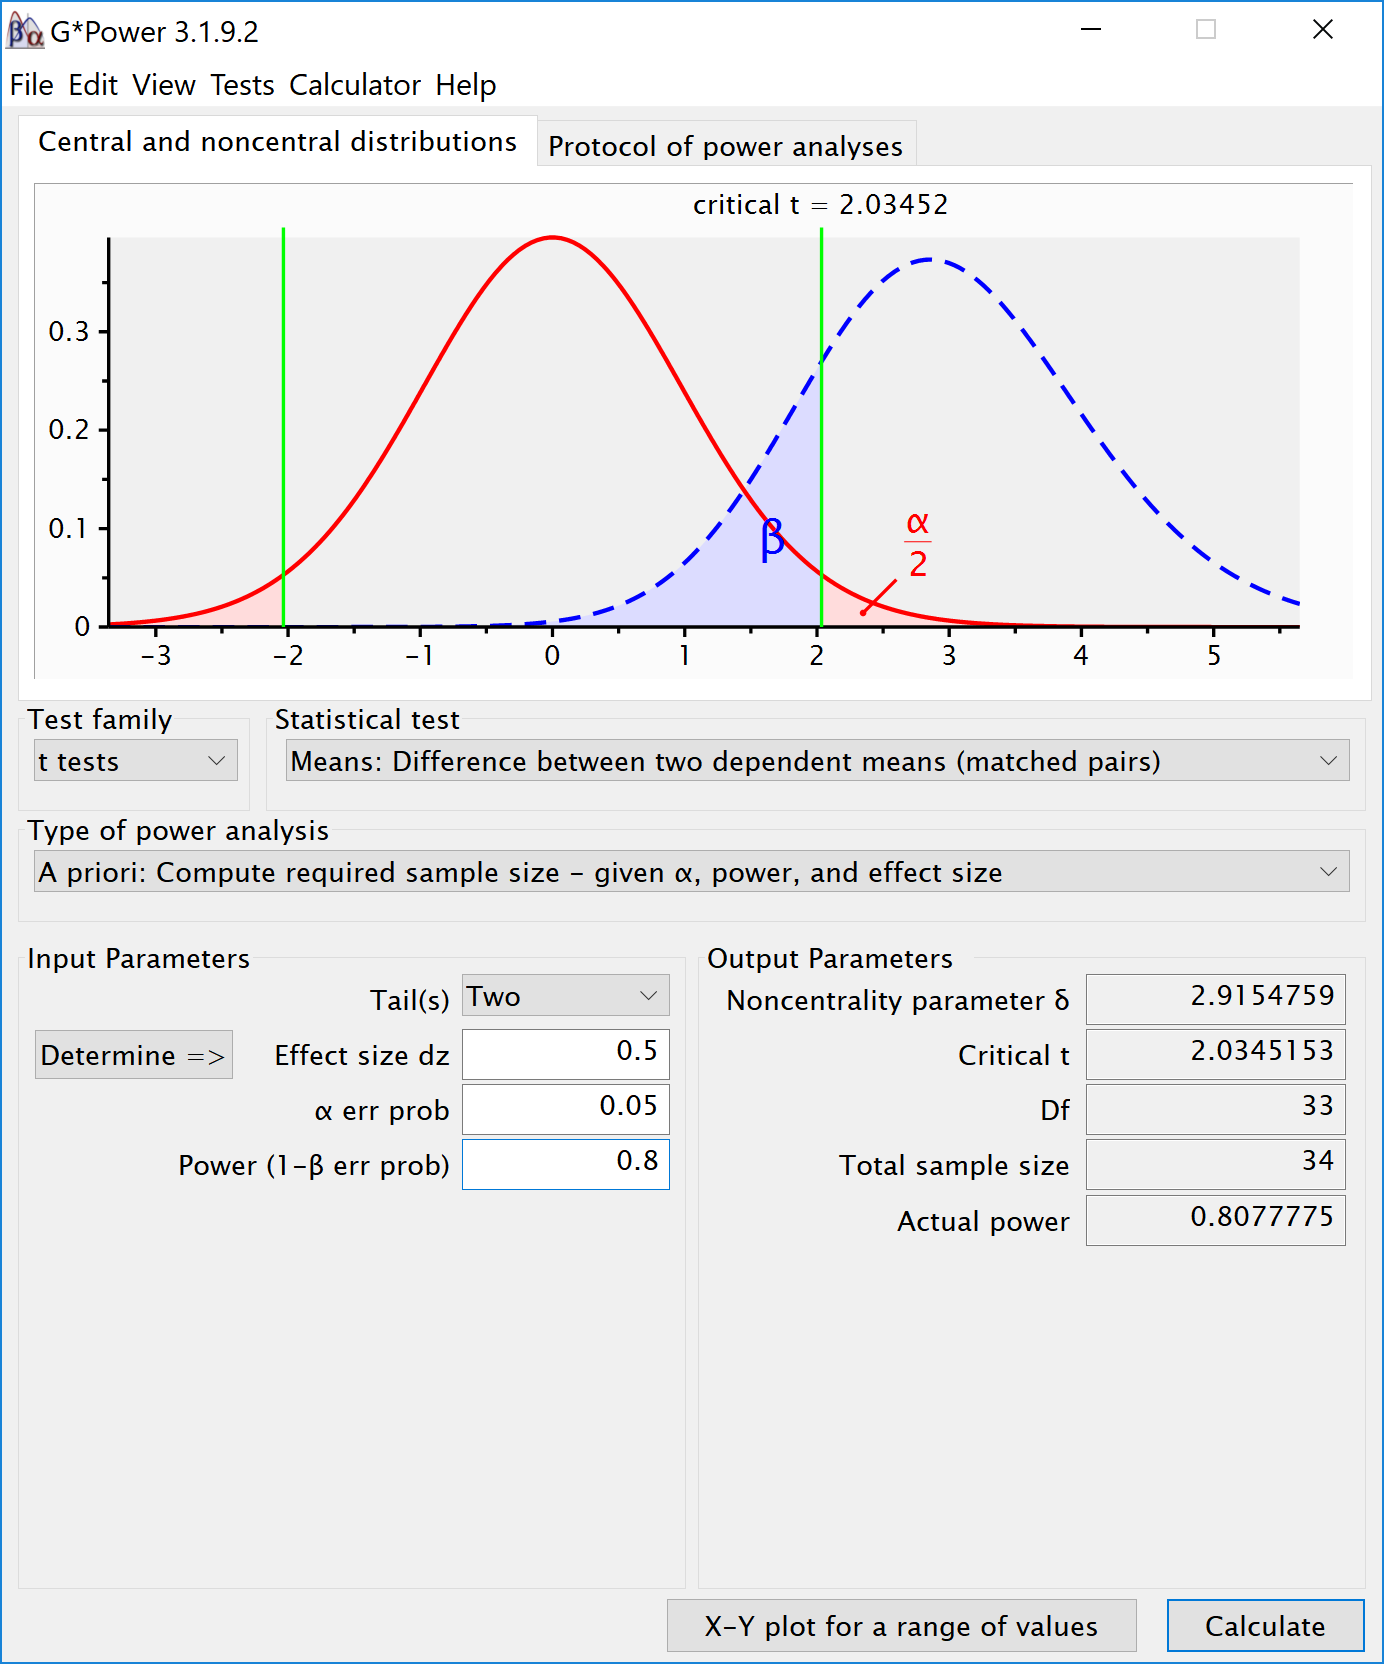
\includegraphics{screenshots/gpower_9.png}

Within designs can have greater power to detect differences than between designs because the values are correlated, and a within design requires less participants because each participant provides multiple observations. One difference between an independent \emph{t}-test and a dependent \emph{t}-test is that an independent \emph{t}-test has 2(n-1) degrees of freedom, while a dependent \emph{t}-test has (n-1) degrees of freedom. The sample size needed in a two-group within-design (NW) relative to the sample needed in two-group between-designs (NB), assuming normal distributions, and ignoring the difference in degrees of freedom between the two types of tests, is (from \citet{maxwell_designing_2004}, p.~561, formula 45):

\(N_{W}=\frac{N_{B}(1-\rho)}{2}\)

The division by 2 in the equation is due to the fact that in a two-condition within design every participant provides two data-points. The extent to which this reduces the sample size compared to a between-subject design depends on the correlation (\emph{r}) between the two dependent variables, as indicated by the \texttt{1-r} part of the equation. If the correlation is 0, a within-subject design needs half as many participants as a between-subject design (e.g., 64 instead 128 participants), simply because every participants provides 2 datapoints. The higher the correlation, the larger the relative benefit of within designs, and whenever the correlation is negative (up to -1) the relative benefit disappears.

Whereas in an independent \emph{t}-test the two observations are uncorrelated, in a within design the observations are correlated. This has an effect on the standard deviation of the difference scores. In turn, because the standardized effect size is the mean difference divided by the standard deviation of the difference scores, the correlation has an effect on the standardized mean difference in a within design, Cohen's dz. The relation, as Cohen (1988, formula 2.3.7) explains, is:

\(\sigma_{z}=\sigma\sqrt{2(1-\rho)}\)

Therefore, the relation between dz and d is \(\sqrt{2(1-\rho)}\). A given difference between population means for matched (dependent) samples is standardized by a value which is \(\sqrt{2(1-\rho)}\) as large as would be the case were they independent. If we enter a correlation of 0.5 in the formula, we get \(\sqrt{2(0.5)}=1\). In other words, when the correlation is 0.5, d = dz. When there is a strong correlation between dependent variables, for example r = 0.9, we get \(d=d_{z}\sqrt{2(1-0.9)}\), and a dz of 1 would be a d = 0.45. Reversely, \(d_{z}=\frac{d}{\sqrt{2(1-r)}}\), so with a r = 0.9, a d of 1 would be a dz = 2.24. Some consider this increase in dz compared to d when observations are strongly correlated an `inflation' when estimating effect sizes, but since the reduction in the standard deviation of the difference scores due to the correlation makes it easier to distinguish signal from noise in a hypothesis test, it leads to a clear power benefit.

\newpage

\begin{Shaded}
\begin{Highlighting}[]
\CommentTok{# Check sample size formula Maxwell}
\CommentTok{# Power is pretty similar with n/2, same d (assuming r = 0.5). }
\CommentTok{# Small differences due to df = 2(n-1) vs df = n-1}
\KeywordTok{pwr.t.test}\NormalTok{(}\DataTypeTok{d =} \FloatTok{0.05}\NormalTok{,}
           \DataTypeTok{n =} \KeywordTok{c}\NormalTok{(}\DecValTok{2000}\NormalTok{, }\DecValTok{4000}\NormalTok{, }\DecValTok{8000}\NormalTok{),}
           \DataTypeTok{sig.level =} \FloatTok{0.05}\NormalTok{,}
           \DataTypeTok{type =} \StringTok{"two.sample"}\NormalTok{,}
           \DataTypeTok{alternative =} \StringTok{"two.sided"}\NormalTok{)}
\end{Highlighting}
\end{Shaded}

\begin{verbatim}
## 
##      Two-sample t test power calculation 
## 
##               n = 2000, 4000, 8000
##               d = 0.05
##       sig.level = 0.05
##           power = 0.3524674, 0.6086764, 0.8853424
##     alternative = two.sided
## 
## NOTE: n is number in *each* group
\end{verbatim}

\begin{Shaded}
\begin{Highlighting}[]
\KeywordTok{pwr.t.test}\NormalTok{(}\DataTypeTok{d =} \FloatTok{0.05}\NormalTok{,}
           \DataTypeTok{n =} \KeywordTok{c}\NormalTok{(}\DecValTok{1000}\NormalTok{, }\DecValTok{2000}\NormalTok{, }\DecValTok{4000}\NormalTok{),}
           \DataTypeTok{sig.level =} \FloatTok{0.05}\NormalTok{,}
           \DataTypeTok{type =} \StringTok{"paired"}\NormalTok{,}
           \DataTypeTok{alternative =} \StringTok{"two.sided"}\NormalTok{)}
\end{Highlighting}
\end{Shaded}

\begin{verbatim}
## 
##      Paired t test power calculation 
## 
##               n = 1000, 2000, 4000
##               d = 0.05
##       sig.level = 0.05
##           power = 0.3520450, 0.6083669, 0.8852320
##     alternative = two.sided
## 
## NOTE: n is number of *pairs*
\end{verbatim}

\newpage

There is no equivalent ``fz'' for Cohen's \emph{f} for a within subject ANOVA. For two groups, we can directly compute Cohen's \emph{f} from Cohen's d for two groups, as \citet{cohen1988spa} describes, because f = 1/2d. For a d = 0.5, f = 0.25. In Gpower we can run a 2 group within-subject power analysis for ANOVA. We plan for 80\% power, and reproduce the anaysis above for the dependent \emph{t}-test. This works because the correlation is set to 0.5, when d = dz, and thus the transformation of f=1/2d works.

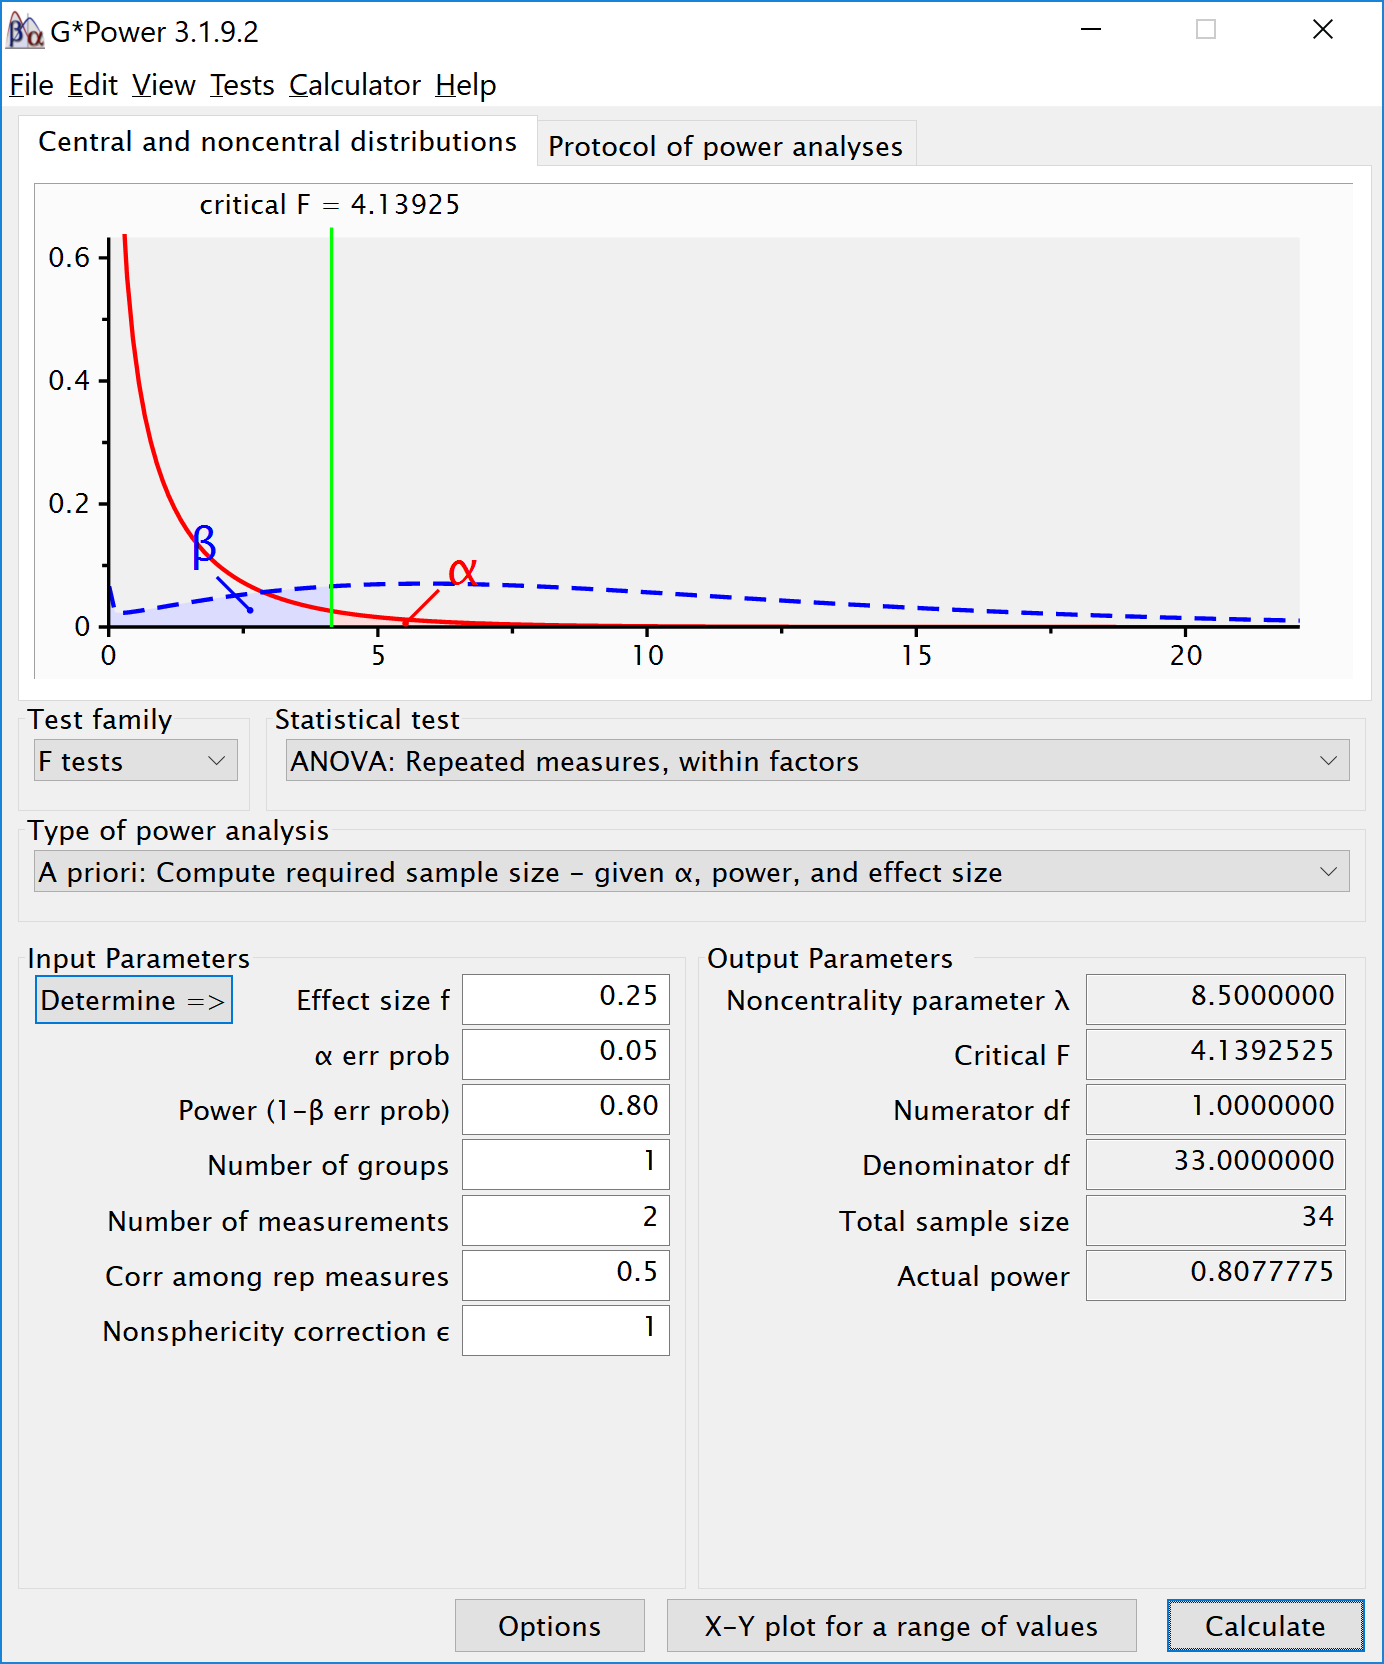
\includegraphics{screenshots/gpower_1.png}

\newpage

If we change the correlation to 0.7 and keep all other settings the same, the repeated measure a-priori power analysis yields a sample of 21. The correlation increases the power for the test.

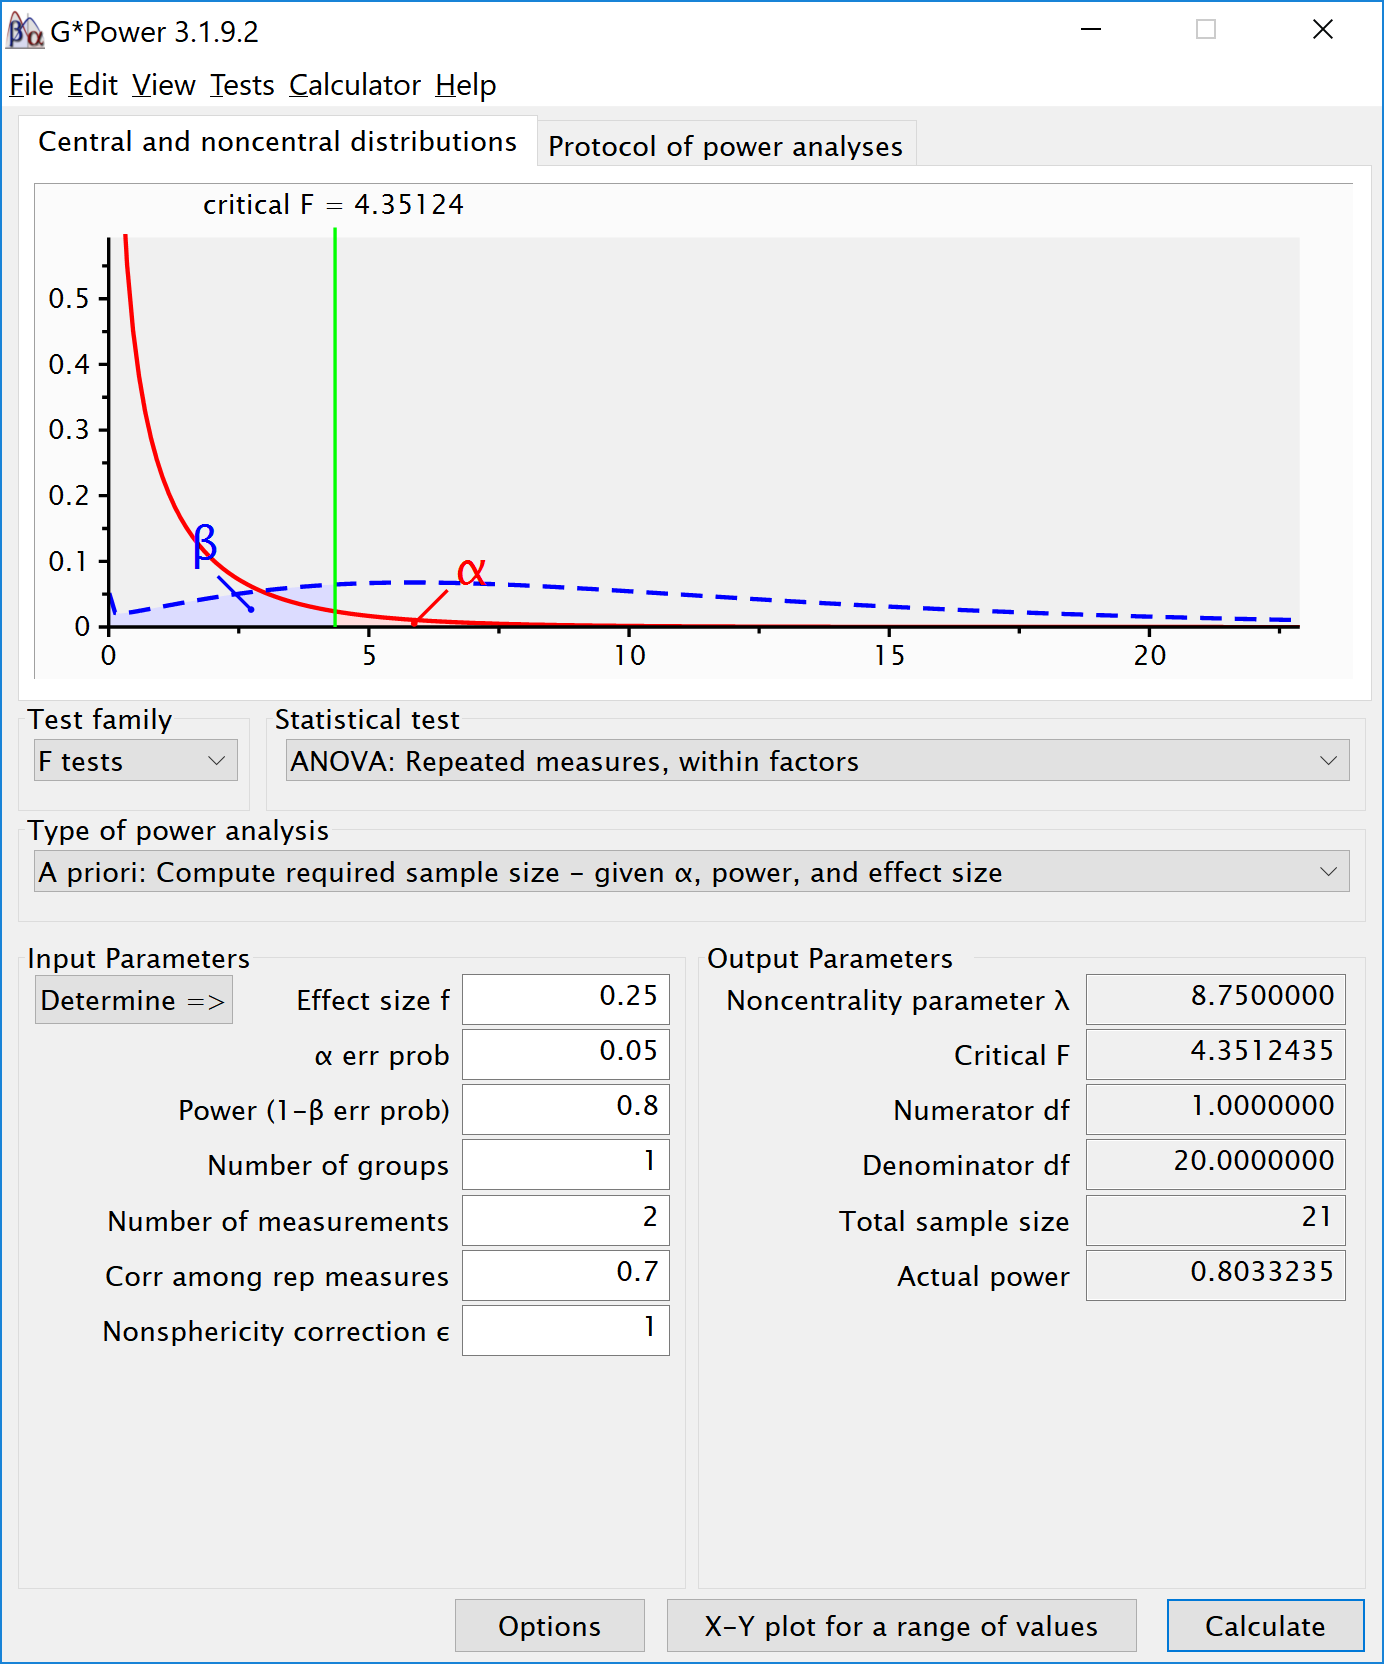
\includegraphics{screenshots/gpower_11.png}

\newpage

To reproduce this analysis in Gpower with a dependent \emph{t}-test we need to change dz following the formula above, \(d_{z}=\frac{0.5}{\sqrt{2(1-0.7)}}\), which yields dz = 0.6454972. If we enter this value in Gpower for an a-priori power analysis, we get the exact same results (as we should, since an repeated measures ANOVA with 2 groups equals a dependent \emph{t}-test). This example illustrates that the correlation between dependent variables always factors into a power analysis, both for a dependent \emph{t}-test, and for a repeated measures ANOVA. Because a dependent \emph{t}-test uses dz the correlation might be less visible, but given the relation between d and dz, the correlation is always taken into account and can greatly improve power for within designs compared to between designs.

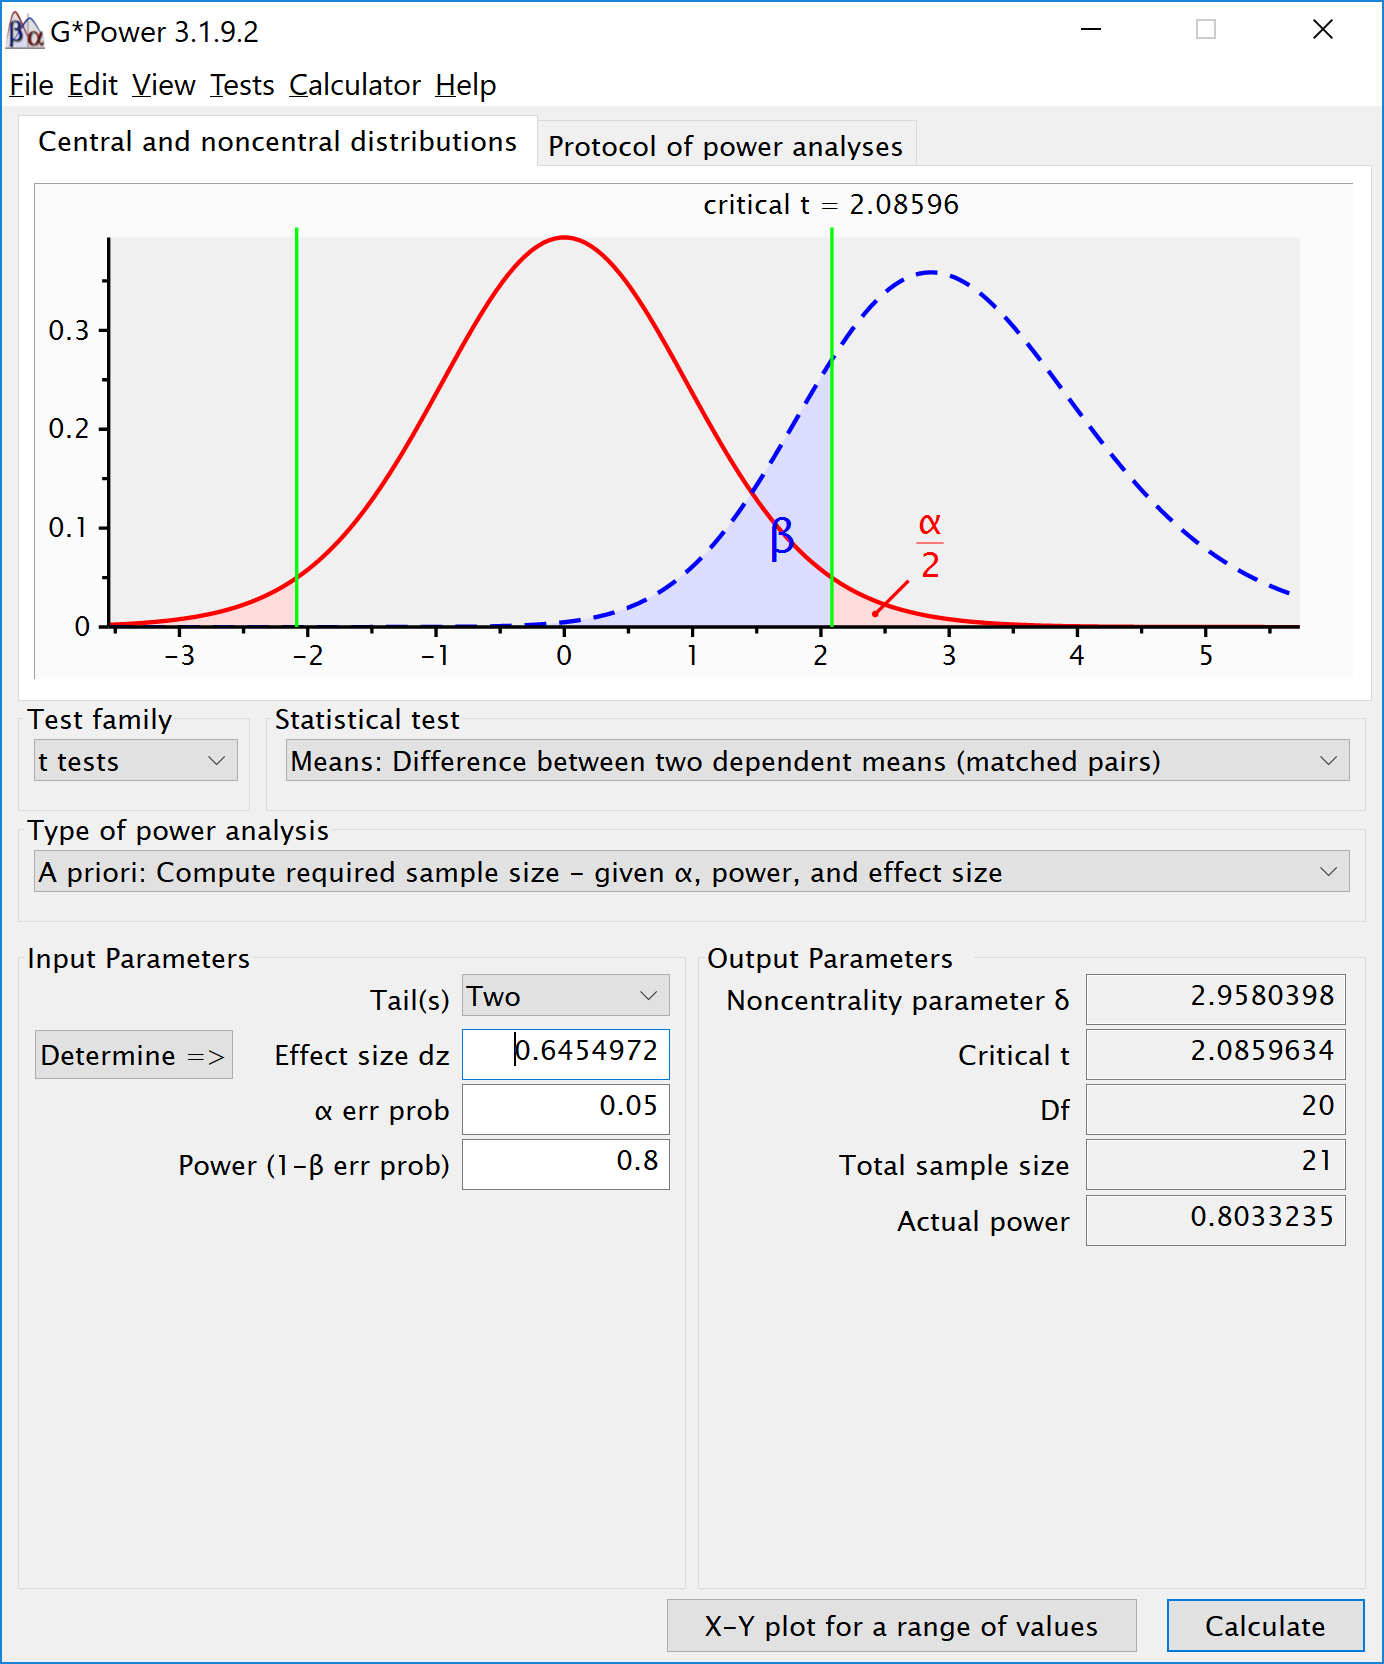
\includegraphics{screenshots/gpower_10.png}

\newpage

We can perform both these power analyses using \texttt{Superpower} as well. We set groups to 2 for the simulation, n = 34 (which should give 80.777 power, according to the \citet{faul2007g} program), a correlation among repeated measures of 0.5, and an alpha of 0.05. In this case, we simulate data with means -0.25 and 0.25, and set the sd to 1. This means we have a mean difference of 0.5, and a Cohen's d of 0.5/1 = 0.5. In the first example, we set the correlation to 0.5, and the result should be 80.77\% power, and an effect size estimate of 0.5 for the simple effect. We also calculate partial eta-squared for the ANOVA, which equals \(\frac{f^2}{f^2+1}\), or 0.05882353.

\begin{Shaded}
\begin{Highlighting}[]
\NormalTok{K <-}\StringTok{ }\DecValTok{2}
\NormalTok{n <-}\StringTok{ }\DecValTok{34}
\NormalTok{sd <-}\StringTok{ }\DecValTok{1}
\NormalTok{r <-}\StringTok{ }\FloatTok{0.5}
\NormalTok{alpha =}\StringTok{ }\FloatTok{0.05}
\NormalTok{f <-}\StringTok{ }\FloatTok{0.25}
\NormalTok{f2 <-}\StringTok{ }\NormalTok{f}\OperatorTok{^}\DecValTok{2}
\NormalTok{ES <-}\StringTok{ }\NormalTok{f2}\OperatorTok{/}\NormalTok{(f2 }\OperatorTok{+}\StringTok{ }\DecValTok{1}\NormalTok{)}
\NormalTok{ES}
\end{Highlighting}
\end{Shaded}

\begin{verbatim}
## [1] 0.05882353
\end{verbatim}

\begin{Shaded}
\begin{Highlighting}[]
\NormalTok{mu <-}\StringTok{ }\KeywordTok{mu_from_ES}\NormalTok{(}\DataTypeTok{K =}\NormalTok{ K, }\DataTypeTok{ES =}\NormalTok{ ES)}
\NormalTok{design =}\StringTok{ }\KeywordTok{paste}\NormalTok{(K,}\StringTok{"w"}\NormalTok{,}\DataTypeTok{sep =} \StringTok{""}\NormalTok{)}
\NormalTok{labelnames <-}\StringTok{ }\KeywordTok{c}\NormalTok{(}\StringTok{"speed"}\NormalTok{, }\StringTok{"fast"}\NormalTok{, }\StringTok{"slow"}\NormalTok{)}
\NormalTok{design_result <-}\StringTok{ }\KeywordTok{ANOVA_design}\NormalTok{(}\DataTypeTok{design =}\NormalTok{ design,}
                   \DataTypeTok{n =}\NormalTok{ n, }\DataTypeTok{mu =}\NormalTok{ mu, }\DataTypeTok{sd =}\NormalTok{ sd, }\DataTypeTok{r =}\NormalTok{ r, }
                   \DataTypeTok{labelnames =}\NormalTok{ labelnames)}
\NormalTok{alpha_level <-}\StringTok{ }\FloatTok{0.05}
\end{Highlighting}
\end{Shaded}

\begin{Shaded}
\begin{Highlighting}[]
\NormalTok{simulation_result <-}\StringTok{ }\KeywordTok{ANOVA_power}\NormalTok{(design_result, }
                                 \DataTypeTok{alpha_level =}\NormalTok{ alpha_level, }
                                 \DataTypeTok{nsims =}\NormalTok{ nsims, }\DataTypeTok{verbose =} \OtherTok{FALSE}\NormalTok{)}
\end{Highlighting}
\end{Shaded}

\newpage

\begin{table}[!h]

\caption{\label{tab:unnamed-chunk-100}Simulated ANOVA Result}
\centering
\begin{tabular}{l|r|r}
\hline
  & power & effect\_size\\
\hline
anova\_speed & 80.74 & 0.2149221\\
\hline
\end{tabular}
\end{table}

\begin{table}[!h]

\caption{\label{tab:unnamed-chunk-102}Exact ANOVA Result}
\centering
\begin{tabular}{l|r|r|r|r}
\hline
  & power & partial\_eta\_squared & cohen\_f & non\_centrality\\
\hline
speed & 80.77775 & 0.2048193 & 0.5075192 & 8.5\\
\hline
\end{tabular}
\end{table}

The results of the simulation are indeed very close to 80.777\%. Note that the simulation calculates Cohen's dz effect sizes for paired comparisons - which here given the correlation of 0.5 is also 0.5 for a medium effect size.

\newpage

We should see a larger dz if we increase the correlation, keeping the sample size the same, following the example in Gpower above. We repeat the simulation, and the only difference is a correlation between dependent variables of 0.7. This should yield an effect size dz = 0.6454972.

\begin{Shaded}
\begin{Highlighting}[]
\NormalTok{K <-}\StringTok{ }\DecValTok{2}
\NormalTok{n <-}\StringTok{ }\DecValTok{21}
\NormalTok{sd <-}\StringTok{ }\DecValTok{1}
\NormalTok{r <-}\StringTok{ }\FloatTok{0.7}
\NormalTok{alpha =}\StringTok{ }\FloatTok{0.05}
\NormalTok{f <-}\StringTok{ }\FloatTok{0.25}
\NormalTok{f2 <-}\StringTok{ }\NormalTok{f}\OperatorTok{^}\DecValTok{2}
\NormalTok{ES <-}\StringTok{ }\NormalTok{f2}\OperatorTok{/}\NormalTok{(f2 }\OperatorTok{+}\StringTok{ }\DecValTok{1}\NormalTok{)}
\NormalTok{ES}
\end{Highlighting}
\end{Shaded}

\begin{verbatim}
## [1] 0.05882353
\end{verbatim}

\begin{Shaded}
\begin{Highlighting}[]
\NormalTok{mu <-}\StringTok{ }\KeywordTok{mu_from_ES}\NormalTok{(}\DataTypeTok{K =}\NormalTok{ K, }\DataTypeTok{ES =}\NormalTok{ ES)}
\NormalTok{design =}\StringTok{ }\KeywordTok{paste}\NormalTok{(K,}\StringTok{"w"}\NormalTok{,}\DataTypeTok{sep =} \StringTok{""}\NormalTok{)}
\NormalTok{labelnames <-}\StringTok{ }\KeywordTok{c}\NormalTok{(}\StringTok{"speed"}\NormalTok{, }\StringTok{"fast"}\NormalTok{, }\StringTok{"slow"}\NormalTok{)}
\NormalTok{design_result <-}\StringTok{ }\KeywordTok{ANOVA_design}\NormalTok{(}\DataTypeTok{design =}\NormalTok{ design,}
                   \DataTypeTok{n =}\NormalTok{ n, }\DataTypeTok{mu =}\NormalTok{ mu, }\DataTypeTok{sd =}\NormalTok{ sd, }\DataTypeTok{r =}\NormalTok{ r, }
                   \DataTypeTok{labelnames =}\NormalTok{ labelnames)}
\NormalTok{alpha_level <-}\StringTok{ }\FloatTok{0.05}
\end{Highlighting}
\end{Shaded}

\begin{table}[!h]

\caption{\label{tab:unnamed-chunk-104}Covariance-Variance Matrix}
\centering
\begin{tabular}{l|r|r}
\hline
  & fast & slow\\
\hline
fast & 1.0 & 0.7\\
\hline
slow & 0.7 & 1.0\\
\hline
\end{tabular}
\end{table}
\newpage

\begin{Shaded}
\begin{Highlighting}[]
\NormalTok{simulation_result <-}\StringTok{ }\KeywordTok{ANOVA_power}\NormalTok{(design_result, }
                                 \DataTypeTok{alpha_level =}\NormalTok{ alpha_level, }
                                 \DataTypeTok{nsims =}\NormalTok{ nsims,}
                                 \DataTypeTok{verbose =} \OtherTok{FALSE}\NormalTok{)}
\end{Highlighting}
\end{Shaded}

\begin{table}[!h]

\caption{\label{tab:unnamed-chunk-106}Simulated ANOVA Result}
\centering
\begin{tabular}{l|r|r}
\hline
  & power & effect\_size\\
\hline
anova\_speed & 80.48 & 0.3153414\\
\hline
\end{tabular}
\end{table}

\begin{Shaded}
\begin{Highlighting}[]
\NormalTok{exact_result <-}\StringTok{ }\KeywordTok{ANOVA_exact}\NormalTok{(design_result,}
                            \DataTypeTok{alpha_level =}\NormalTok{ alpha_level,}
                            \DataTypeTok{verbose =} \OtherTok{FALSE}\NormalTok{)}
\end{Highlighting}
\end{Shaded}

\begin{table}[!h]

\caption{\label{tab:unnamed-chunk-108}Exact ANOVA Result}
\centering
\begin{tabular}{l|r|r|r|r}
\hline
  & power & partial\_eta\_squared & cohen\_f & non\_centrality\\
\hline
speed & 80.33235 & 0.3043478 & 0.6614378 & 8.75\\
\hline
\end{tabular}
\end{table}

\begin{Shaded}
\begin{Highlighting}[]
\CommentTok{#relation dz and f for within designs }
\NormalTok{f <-}\StringTok{ }\FloatTok{0.5}\OperatorTok{*}\FloatTok{0.6454972}
\NormalTok{f }
\end{Highlighting}
\end{Shaded}

\begin{verbatim}
## [1] 0.3227486
\end{verbatim}

Entering this f in Gpower, with a correlation of 0.5, yields the same as entering \texttt{f\ =\ 0.25} and \texttt{correlation\ =\ 0.7}.

\newpage

\hypertarget{part-2}{%
\section{Part 2}\label{part-2}}

Here, we will examine a repeated measures experiment with 3 within-subject conditions, to illustrate how a repeated measures ANOVA extends a dependent \emph{t}-test with 3 groups.

In the example for a two-group within design we provided a specific formula for the sample size benefit for two groups. The sample size needed in within-designs (NW) with more than 2 conditions, relative to the sample needed in between-designs (NB), assuming normal distributions and compound symmetry, and ignoring the difference in degrees of freedom between the two types of tests, is (from \citet{maxwell_designing_2004}, p.~562, formula 47):

\(N_{W}=\frac{N_{B}(1-\rho)}{a}\)

Where ``a'' is the number of within-subject levels.

\hypertarget{the-relation-between-cohens-f-and-cohens-d}{%
\subsection{The relation between Cohen's f and Cohen's d}\label{the-relation-between-cohens-f-and-cohens-d}}

Whereas in the case of a repeated measures ANOVA with 2 groups we could explain the principles of a power analysis by comparing our test against a \emph{t}-test and Cohen's d, this becomes more difficult when we have more than 2 groups. It is more useful to explain how to directly calculate Cohen's \emph{f}, the effect size used in power analyses for ANOVA. Cohen's \emph{f} is calculated following \citet{cohen1988spa}, formula 8.2.1 and 8.2.2:

\(f = \sqrt{\frac{\frac{\sum(\mu-\overline{\mu})^2)}N}\sigma}\)

Imagine we have a within-subject experiment with 3 conditions. We ask people what they mood is when their alarm clock wakes them up, when they wake up naturally on a week day, and when they wake up naturally on a weekend day. Based on pilot data, we expect the means (on a 7 point validated mood scale) are 3.8, 4.2, and 4.3. The standard deviation is 0.9, and the correlation between the dependent measurements is 0.7. We can calculate Cohen's \emph{f} for the ANOVA, and Cohen's dz for the contrasts:

\begin{Shaded}
\begin{Highlighting}[]
\NormalTok{mu <-}\StringTok{ }\KeywordTok{c}\NormalTok{(}\FloatTok{3.8}\NormalTok{, }\FloatTok{4.2}\NormalTok{, }\FloatTok{4.3}\NormalTok{)}
\NormalTok{sd <-}\StringTok{ }\FloatTok{0.9}
\NormalTok{f <-}\StringTok{ }\KeywordTok{sqrt}\NormalTok{(}\KeywordTok{sum}\NormalTok{((mu }\OperatorTok{-}\StringTok{ }\KeywordTok{mean}\NormalTok{(mu)) }\OperatorTok{^}\StringTok{ }\DecValTok{2}\NormalTok{) }\OperatorTok{/}\StringTok{ }\KeywordTok{length}\NormalTok{(mu)) }\OperatorTok{/}\StringTok{ }\NormalTok{sd }
\CommentTok{#Cohen, 1988, formula 8.2.1 and 8.2.2}
\NormalTok{  f}
\end{Highlighting}
\end{Shaded}

\begin{verbatim}
## [1] 0.2400274
\end{verbatim}

\begin{Shaded}
\begin{Highlighting}[]
\NormalTok{  r <-}\StringTok{ }\FloatTok{0.7}
\NormalTok{  (}\FloatTok{4.2} \OperatorTok{-}\StringTok{ }\FloatTok{3.8}\NormalTok{) }\OperatorTok{/}\StringTok{ }\FloatTok{0.9} \OperatorTok{/}\StringTok{ }\KeywordTok{sqrt}\NormalTok{(}\DecValTok{2} \OperatorTok{*}\StringTok{ }\NormalTok{(}\DecValTok{1} \OperatorTok{-}\StringTok{ }\NormalTok{r))}
\end{Highlighting}
\end{Shaded}

\begin{verbatim}
## [1] 0.5737753
\end{verbatim}

\begin{Shaded}
\begin{Highlighting}[]
\NormalTok{  (}\FloatTok{4.3} \OperatorTok{-}\StringTok{ }\FloatTok{3.8}\NormalTok{) }\OperatorTok{/}\StringTok{ }\FloatTok{0.9} \OperatorTok{/}\StringTok{ }\KeywordTok{sqrt}\NormalTok{(}\DecValTok{2} \OperatorTok{*}\StringTok{ }\NormalTok{(}\DecValTok{1} \OperatorTok{-}\StringTok{ }\NormalTok{r))}
\end{Highlighting}
\end{Shaded}

\begin{verbatim}
## [1] 0.7172191
\end{verbatim}

\begin{Shaded}
\begin{Highlighting}[]
\NormalTok{  (}\FloatTok{4.3} \OperatorTok{-}\StringTok{ }\FloatTok{4.2}\NormalTok{) }\OperatorTok{/}\StringTok{ }\FloatTok{0.9} \OperatorTok{/}\StringTok{ }\KeywordTok{sqrt}\NormalTok{(}\DecValTok{2} \OperatorTok{*}\StringTok{ }\NormalTok{(}\DecValTok{1} \OperatorTok{-}\StringTok{ }\NormalTok{r))}
\end{Highlighting}
\end{Shaded}

\begin{verbatim}
## [1] 0.1434438
\end{verbatim}

The relation between Cohen's d or dz and Cohen's \emph{f} becomes more difficult when there are multiple groups, because the relationship depends on the pattern of the means. \citet{cohen1988spa} presents calculations for three patterns, minimal variability (for example, for 5 means: -0.25, 0, 0, 0, 0.25), medium variability (for example, for 5 means: -0.25, -0.25, 0.25, 0.25, 0.25 or -0.25, -0.25, -0.25, 0.25, 0.25). For these three patterns, formula's are available that compute Cohen's \emph{f} from Cohen's d, where d is the effect size calculated for the difference between the largest and smallest mean (if the largest mean is 0.25 and the smallest mean is -0.25, 0.25 - -0.25 = 0.5, so d is 0.5 divided by the standard deviation of 0.9). In our example, d would be (4.3-3.8)/0.9 = 0.5555556. If we divide this value by \texttt{sqrt(2*(1-r))} we have dz = 0.5555556/0.7745967 = 0.7172191.

We have created a custom function that will calculate f from d, based on a specification of one of the three patterns of means. Our pattern is most similar (but not identical) to a maximum variability pattern (two means are high, one is lower). So we could attempt to calculate f from d (0.5555556), by calculating d from the largest and smallest mean.

This function allows you to calculate f, d and eta squared
following \citet{cohen1988spa}, p 277. The patterns are:
1. Minimum variability: one mean at each end of d, the remaining k- 2 means all at the midpoint.
2. Intermediate variability: the k means equally spaced over d.
3. Maximum variability: the means all at the end points of d.

For each of these patterns, there is a fixed relationship between f and d for any given number of means, k.

\textbf{Pattern 1}
For any given range of means, d, the minimum standard deviation, f1, results when the remaining k - 2 means are concentrated at the mean of the means (0 when expressed in standard units), i.e., half-way between the largest and smallest.

\textbf{Pattern 2}
A pattern of medium variability results when the k meansare equally spaced over the range, and therefore at intervals of d/(k- 1).

\textbf{Pattern 3}
It is demonstrable and intuitively evident that for any given range the dispersion which yield\textasciitilde{} the maximum standard deviation has the k means falling at both extremes of the range. When k is even, !k fall at - !d and the other !k fall at + !d; when k is odd, (k + I )/2 of the means fall at either end and the (k- 1)/2 remaining means at the other. With this pattern, for all even numbers of means, use formula (8.2.12). When k is odd, and there is thus one more mean at one extreme than at the other, use formula (8.2.13).

\begin{Shaded}
\begin{Highlighting}[]
\NormalTok{calc_f_d_eta <-}\StringTok{ }\ControlFlowTok{function}\NormalTok{(mu, sd, variability)\{}
  \ControlFlowTok{if}\NormalTok{ (variability }\OperatorTok{==}\StringTok{ "minimum"}\NormalTok{) \{}
\NormalTok{    k =}\StringTok{ }\KeywordTok{length}\NormalTok{(mu)}
\NormalTok{    d <-}\StringTok{ }\NormalTok{(}\KeywordTok{max}\NormalTok{(mu) }\OperatorTok{-}\StringTok{ }\KeywordTok{min}\NormalTok{(mu)) }\OperatorTok{/}\StringTok{ }\NormalTok{sd}
\NormalTok{    f <-}\StringTok{ }\NormalTok{d }\OperatorTok{*}\StringTok{ }\KeywordTok{sqrt}\NormalTok{(}\DecValTok{1} \OperatorTok{/}\StringTok{ }\NormalTok{(}\DecValTok{2} \OperatorTok{*}\StringTok{ }\NormalTok{k))}
\NormalTok{    f2 <-}\StringTok{ }\NormalTok{f }\OperatorTok{^}\StringTok{ }\DecValTok{2}
\NormalTok{    ES <-}\StringTok{ }\NormalTok{f2 }\OperatorTok{/}\StringTok{ }\NormalTok{(f2 }\OperatorTok{+}\StringTok{ }\DecValTok{1}\NormalTok{)}
\NormalTok{  \}}
  \ControlFlowTok{if}\NormalTok{ (variability }\OperatorTok{==}\StringTok{ "medium"}\NormalTok{) \{}
\NormalTok{    k =}\StringTok{ }\KeywordTok{length}\NormalTok{(mu)}
\NormalTok{    d <-}\StringTok{ }\NormalTok{(}\KeywordTok{max}\NormalTok{(mu) }\OperatorTok{-}\StringTok{ }\KeywordTok{min}\NormalTok{(mu)) }\OperatorTok{/}\StringTok{ }\NormalTok{sd}
\NormalTok{    f <-}\StringTok{ }\NormalTok{(d }\OperatorTok{/}\StringTok{ }\DecValTok{2}\NormalTok{) }\OperatorTok{*}\StringTok{ }\KeywordTok{sqrt}\NormalTok{((k }\OperatorTok{+}\StringTok{ }\DecValTok{1}\NormalTok{) }\OperatorTok{/}\StringTok{ }\NormalTok{(}\DecValTok{3} \OperatorTok{*}\StringTok{ }\NormalTok{(k }\OperatorTok{-}\StringTok{ }\DecValTok{1}\NormalTok{)))}
\NormalTok{    f2 <-}\StringTok{ }\NormalTok{f }\OperatorTok{^}\StringTok{ }\DecValTok{2}
\NormalTok{    ES <-}\StringTok{ }\NormalTok{f2 }\OperatorTok{/}\StringTok{ }\NormalTok{(f2 }\OperatorTok{+}\StringTok{ }\DecValTok{1}\NormalTok{)}
\NormalTok{  \}}
  \ControlFlowTok{if}\NormalTok{ (variability }\OperatorTok{==}\StringTok{ "maximum"}\NormalTok{) \{}
\NormalTok{    k =}\StringTok{ }\KeywordTok{length}\NormalTok{(mu)}
\NormalTok{    d <-}\StringTok{ }\NormalTok{(}\KeywordTok{max}\NormalTok{(mu) }\OperatorTok{-}\StringTok{ }\KeywordTok{min}\NormalTok{(mu)) }\OperatorTok{/}\StringTok{ }\NormalTok{sd}
\NormalTok{    f <-}\StringTok{ }\KeywordTok{ifelse}\NormalTok{(k }\OperatorTok\StringTok{ }\DecValTok{2} \OperatorTok{==}\StringTok{ }\DecValTok{0}\NormalTok{, }\FloatTok{.5} \OperatorTok{*}\StringTok{ }\NormalTok{d, d }\OperatorTok{*}\StringTok{ }\NormalTok{(}\KeywordTok{sqrt}\NormalTok{(k }\OperatorTok{^}\StringTok{ }\DecValTok{2} \OperatorTok{-}\StringTok{ }\DecValTok{1}\NormalTok{) }\OperatorTok{/}\StringTok{ }\NormalTok{(}\DecValTok{2} \OperatorTok{*}\StringTok{ }\NormalTok{k)))}
\NormalTok{    f2 <-}\StringTok{ }\NormalTok{f }\OperatorTok{^}\StringTok{ }\DecValTok{2}
\NormalTok{    ES <-}\StringTok{ }\NormalTok{f2 }\OperatorTok{/}\StringTok{ }\NormalTok{(f2 }\OperatorTok{+}\StringTok{ }\DecValTok{1}\NormalTok{)}
\NormalTok{  \}}
  \KeywordTok{invisible}\NormalTok{(}\KeywordTok{list}\NormalTok{(}\DataTypeTok{mu =}\NormalTok{ mu,}
                 \DataTypeTok{sd =}\NormalTok{ sd,}
                 \DataTypeTok{d =}\NormalTok{ d,}
                 \DataTypeTok{f =}\NormalTok{ f,}
                 \DataTypeTok{f2 =}\NormalTok{ f2,}
                 \DataTypeTok{ES =}\NormalTok{ ES))}
\NormalTok{\}}
\NormalTok{res <-}\StringTok{ }\KeywordTok{calc_f_d_eta}\NormalTok{(}\DataTypeTok{mu =}\NormalTok{ mu, }\DataTypeTok{sd =}\NormalTok{ sd, }\DataTypeTok{variability =} \StringTok{"maximum"}\NormalTok{)}
\NormalTok{res}\OperatorTok{$}\NormalTok{f}
\end{Highlighting}
\end{Shaded}

\begin{verbatim}
## [1] 0.2618914
\end{verbatim}

\begin{Shaded}
\begin{Highlighting}[]
\NormalTok{res}\OperatorTok{$}\NormalTok{d}
\end{Highlighting}
\end{Shaded}

\begin{verbatim}
## [1] 0.5555556
\end{verbatim}

We see the Cohen's \emph{f} value is 0.2618914 and d = 0.5555556. The Cohen's \emph{f} is not perfectly accurate - it is assuming the pattern of means is 3.8, 4.3, 4.3, and not 3.8, 4.2, 4.3. If the means and sd is known, it is best to calculate Cohen's \emph{f} directly from these values.

\hypertarget{three-within-conditions-medium-effect-size}{%
\subsection{Three within conditions, medium effect size}\label{three-within-conditions-medium-effect-size}}

We can perform power analyses for within designs using simuations. We set groups to 3 for the simulation, n = 20, and the correlation between dependent variables to 0.8. If the true effect size is f = 0.25, and the alpha level is 0.05, the power is 96.6\%. In this case, we simulate data with means -0.3061862, 0.0000000, and 0.3061862, and set the sd to 1.

\begin{Shaded}
\begin{Highlighting}[]
\NormalTok{K <-}\StringTok{ }\DecValTok{3}
\NormalTok{n <-}\StringTok{ }\DecValTok{20}
\NormalTok{sd <-}\StringTok{ }\DecValTok{1}
\NormalTok{r <-}\StringTok{ }\FloatTok{0.8}
\NormalTok{alpha =}\StringTok{ }\FloatTok{0.05}
\NormalTok{f <-}\StringTok{ }\FloatTok{0.25}
\NormalTok{f2 <-}\StringTok{ }\NormalTok{f}\OperatorTok{^}\DecValTok{2}
\NormalTok{ES <-}\StringTok{ }\NormalTok{f2 }\OperatorTok{/}\StringTok{ }\NormalTok{(f2 }\OperatorTok{+}\StringTok{ }\DecValTok{1}\NormalTok{)}
\NormalTok{ES}
\end{Highlighting}
\end{Shaded}

\begin{verbatim}
## [1] 0.05882353
\end{verbatim}

\begin{Shaded}
\begin{Highlighting}[]
\NormalTok{mu <-}\StringTok{ }\KeywordTok{mu_from_ES}\NormalTok{(}\DataTypeTok{K =}\NormalTok{ K, }\DataTypeTok{ES =}\NormalTok{ ES)}

\CommentTok{#Cohen, 1988, formula 8.2.1 and 8.2.2}
\KeywordTok{sqrt}\NormalTok{(}\KeywordTok{sum}\NormalTok{((mu }\OperatorTok{-}\StringTok{ }\KeywordTok{mean}\NormalTok{(mu)) }\OperatorTok{^}\StringTok{ }\DecValTok{2}\NormalTok{) }\OperatorTok{/}\StringTok{ }\KeywordTok{length}\NormalTok{(mu)) }\OperatorTok{/}\StringTok{ }\NormalTok{sd }
\end{Highlighting}
\end{Shaded}

\begin{verbatim}
## [1] 0.25
\end{verbatim}

\begin{Shaded}
\begin{Highlighting}[]
\NormalTok{design =}\StringTok{ }\KeywordTok{paste}\NormalTok{(K, }\StringTok{"w"}\NormalTok{, }\DataTypeTok{sep =} \StringTok{""}\NormalTok{)}
\NormalTok{labelnames <-}\StringTok{ }\KeywordTok{c}\NormalTok{(}\StringTok{"speed"}\NormalTok{, }\StringTok{"fast"}\NormalTok{, }\StringTok{"medium"}\NormalTok{, }\StringTok{"slow"}\NormalTok{)}
\NormalTok{design_result <-}\StringTok{ }\KeywordTok{ANOVA_design}\NormalTok{(}\DataTypeTok{design =}\NormalTok{ design,}
                   \DataTypeTok{n =}\NormalTok{ n, }
                   \DataTypeTok{mu =}\NormalTok{ mu, }
                   \DataTypeTok{sd =}\NormalTok{ sd, }
                   \DataTypeTok{r =}\NormalTok{ r, }
                   \DataTypeTok{labelnames =}\NormalTok{ labelnames)}

\NormalTok{alpha_level <-}\StringTok{ }\FloatTok{0.05}
\end{Highlighting}
\end{Shaded}

\begin{Shaded}
\begin{Highlighting}[]
\NormalTok{simulation_result <-}\StringTok{ }\KeywordTok{ANOVA_power}\NormalTok{(design_result, }
                                 \DataTypeTok{alpha_level =}\NormalTok{ alpha_level, }
                                 \DataTypeTok{nsims =}\NormalTok{ nsims,}
                                 \DataTypeTok{verbose =} \OtherTok{FALSE}\NormalTok{)}
\end{Highlighting}
\end{Shaded}

\begin{table}[!h]

\caption{\label{tab:unnamed-chunk-114}Simulated ANOVA Result}
\centering
\begin{tabular}{l|r|r}
\hline
  & power & effect\_size\\
\hline
anova\_speed & 97.04 & 0.345486\\
\hline
\end{tabular}
\end{table}

\begin{Shaded}
\begin{Highlighting}[]
\NormalTok{exact_result <-}\StringTok{ }\KeywordTok{ANOVA_exact}\NormalTok{(design_result,}
                            \DataTypeTok{alpha_level =}\NormalTok{ alpha_level,}
                            \DataTypeTok{verbose =} \OtherTok{FALSE}\NormalTok{)}
\end{Highlighting}
\end{Shaded}

\begin{table}[!h]

\caption{\label{tab:unnamed-chunk-116}Exact ANOVA Result}
\centering
\begin{tabular}{l|r|r|r|r}
\hline
  & power & partial\_eta\_squared & cohen\_f & non\_centrality\\
\hline
speed & 96.91634 & 0.3303965 & 0.7024394 & 18.75\\
\hline
\end{tabular}
\end{table}

The results of the simulation are indeed very close to 96.9\%.
\newpage

We can see this is in line with the power estimate from Gpower:

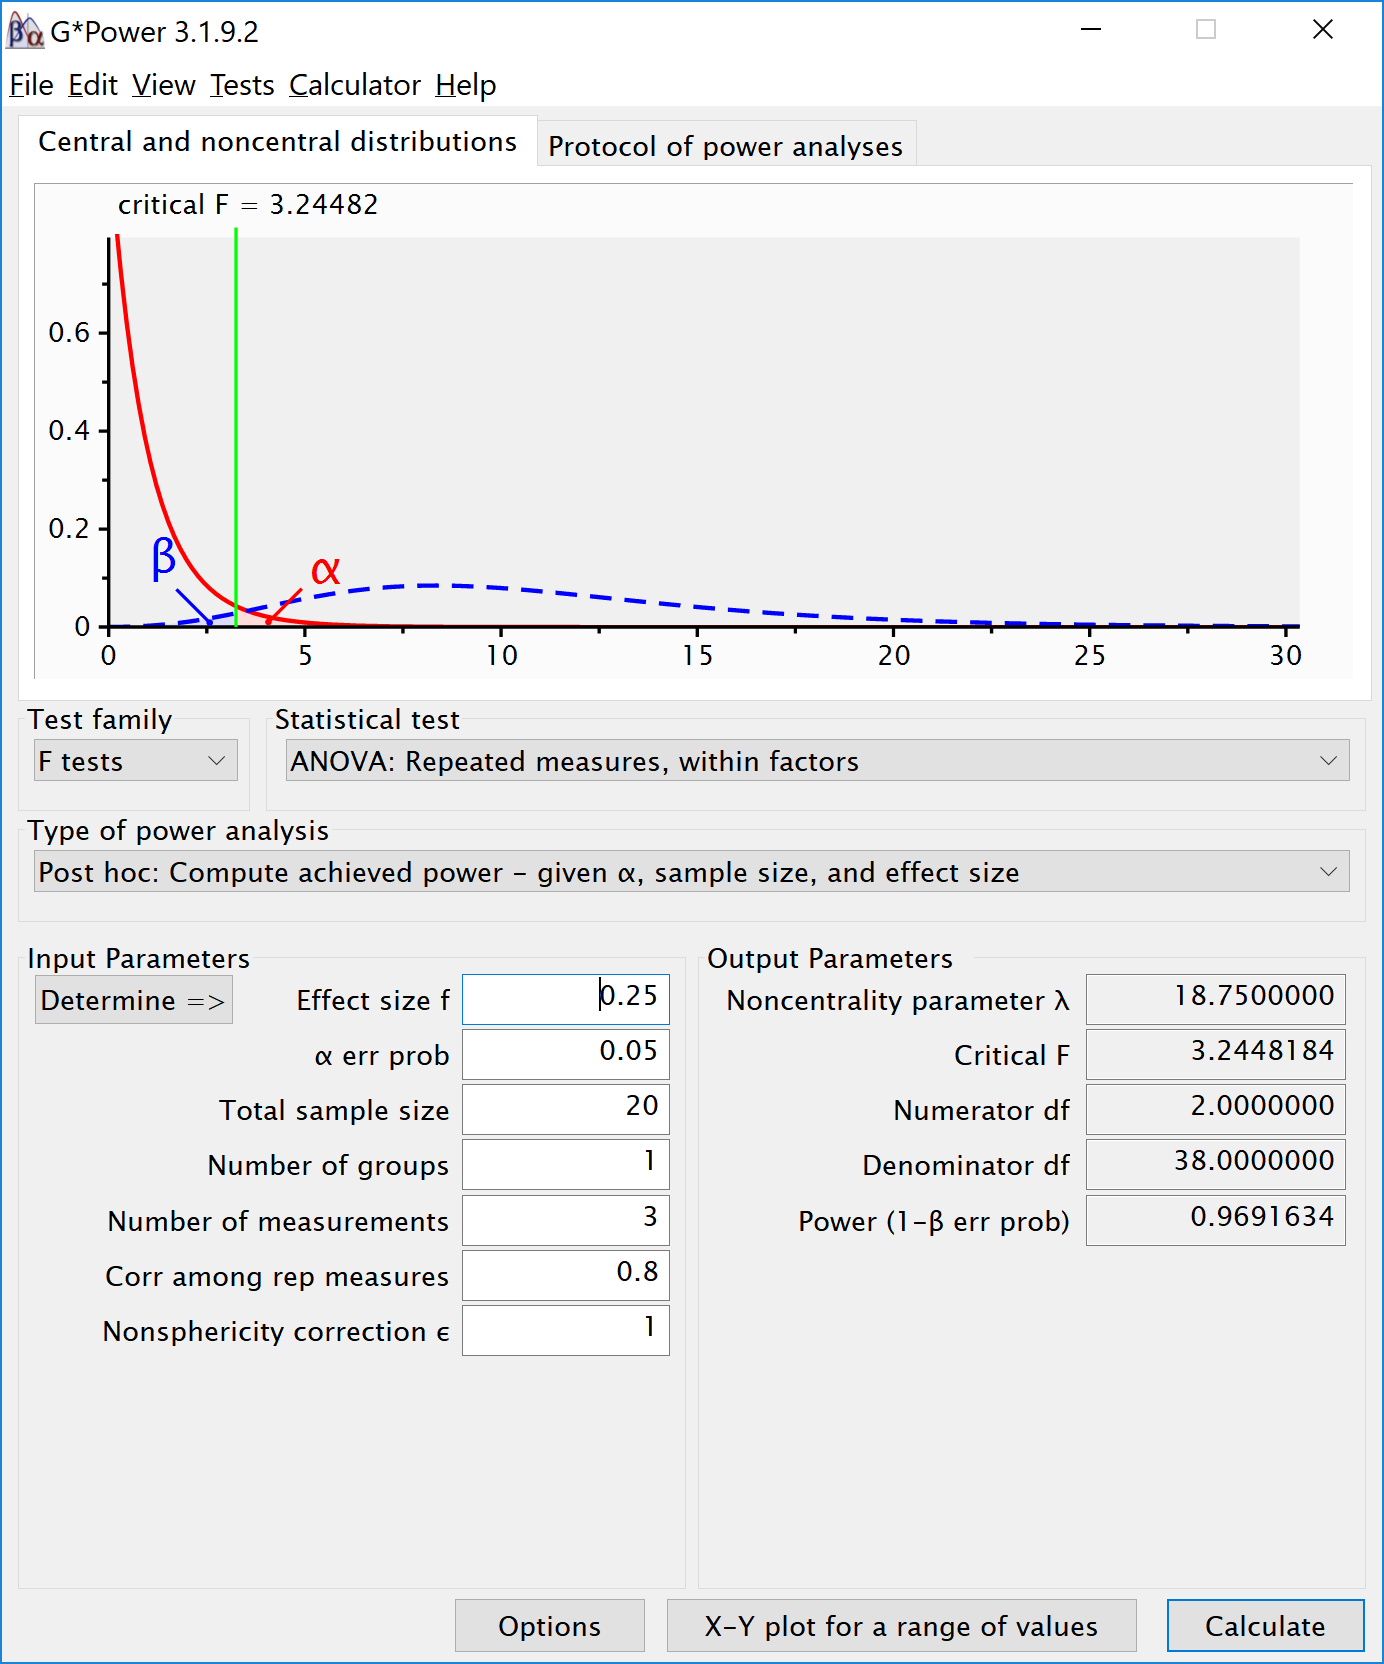
\includegraphics{screenshots/gpower_12.png}

\newpage

We can also validate this by creating the code to do a power analysis in R from scratch:

\begin{Shaded}
\begin{Highlighting}[]
\NormalTok{K <-}\StringTok{ }\DecValTok{3} \CommentTok{#three groups}
\NormalTok{n <-}\StringTok{ }\DecValTok{20}
\NormalTok{sd <-}\StringTok{ }\DecValTok{1}
\NormalTok{r <-}\StringTok{ }\FloatTok{0.8}
\NormalTok{alpha =}\StringTok{ }\FloatTok{0.05}
\NormalTok{f <-}\StringTok{ }\FloatTok{0.25}
\NormalTok{f2 <-}\StringTok{ }\NormalTok{f}\OperatorTok{^}\DecValTok{2}
\NormalTok{ES <-}\StringTok{ }\NormalTok{f2 }\OperatorTok{/}\StringTok{ }\NormalTok{(f2 }\OperatorTok{+}\StringTok{ }\DecValTok{1}\NormalTok{)}
\NormalTok{ES}
\end{Highlighting}
\end{Shaded}

\begin{verbatim}
## [1] 0.05882353
\end{verbatim}

\begin{Shaded}
\begin{Highlighting}[]
\NormalTok{mu <-}\StringTok{ }\KeywordTok{mu_from_ES}\NormalTok{(}\DataTypeTok{K =}\NormalTok{ K, }\DataTypeTok{ES =}\NormalTok{ ES)}
\NormalTok{design =}\StringTok{ }\KeywordTok{paste}\NormalTok{(K, }\StringTok{"w"}\NormalTok{, }\DataTypeTok{sep =} \StringTok{""}\NormalTok{)}
\NormalTok{labelnames <-}\StringTok{ }\KeywordTok{c}\NormalTok{(}\StringTok{"speed"}\NormalTok{, }\StringTok{"fast"}\NormalTok{, }\StringTok{"medium"}\NormalTok{, }\StringTok{"slow"}\NormalTok{)}
\NormalTok{design_result <-}\StringTok{ }\KeywordTok{ANOVA_design}\NormalTok{(}\DataTypeTok{design =}\NormalTok{ design,}
                   \DataTypeTok{n =}\NormalTok{ n, }
                   \DataTypeTok{mu =}\NormalTok{ mu, }
                   \DataTypeTok{sd =}\NormalTok{ sd, }
                   \DataTypeTok{r =}\NormalTok{ r, }
                   \DataTypeTok{labelnames =}\NormalTok{ labelnames)}

\KeywordTok{power_oneway_within}\NormalTok{(design_result)}\OperatorTok{$}\NormalTok{power}
\end{Highlighting}
\end{Shaded}

\begin{verbatim}
## [1] 96.91634
\end{verbatim}

\begin{Shaded}
\begin{Highlighting}[]
\KeywordTok{power_oneway_within}\NormalTok{(design_result)}\OperatorTok{$}\NormalTok{eta_p_}\DecValTok{2}
\end{Highlighting}
\end{Shaded}

\begin{verbatim}
## [1] 0.05882353
\end{verbatim}

\begin{Shaded}
\begin{Highlighting}[]
\KeywordTok{power_oneway_within}\NormalTok{(design_result)}\OperatorTok{$}\NormalTok{eta_p_}\DecValTok{2}\NormalTok{_SPSS}
\end{Highlighting}
\end{Shaded}

\begin{verbatim}
## [1] 0.3303965
\end{verbatim}

\begin{Shaded}
\begin{Highlighting}[]
\KeywordTok{power_oneway_within}\NormalTok{(design_result)}\OperatorTok{$}\NormalTok{Cohen_f}
\end{Highlighting}
\end{Shaded}

\begin{verbatim}
## [1] 0.25
\end{verbatim}

\begin{Shaded}
\begin{Highlighting}[]
\KeywordTok{power_oneway_within}\NormalTok{(design_result)}\OperatorTok{$}\NormalTok{Cohen_f_SPSS}
\end{Highlighting}
\end{Shaded}

\begin{verbatim}
## [1] 0.7024394
\end{verbatim}

\newpage

We can even check the calculation of Cohen's \emph{f} SPSS style in GPower. We take the GPower settings as illustrated above. We click the `Options' button, and check the radiobutton next to `As in SPSS'. Click ok, and you will notice that the `Corr among rep measures' field has disappeared. The correlation does not need to be entered seperately, but is incorporated in Cohen's \emph{f}. The value of Cohen's \emph{f}, which was 0.25, has changed into 0.7024394. This is the SPSS equivalent. The value is much larger. This value, and it's corresponding partial eta-squared, incorporate the correlation between observations.

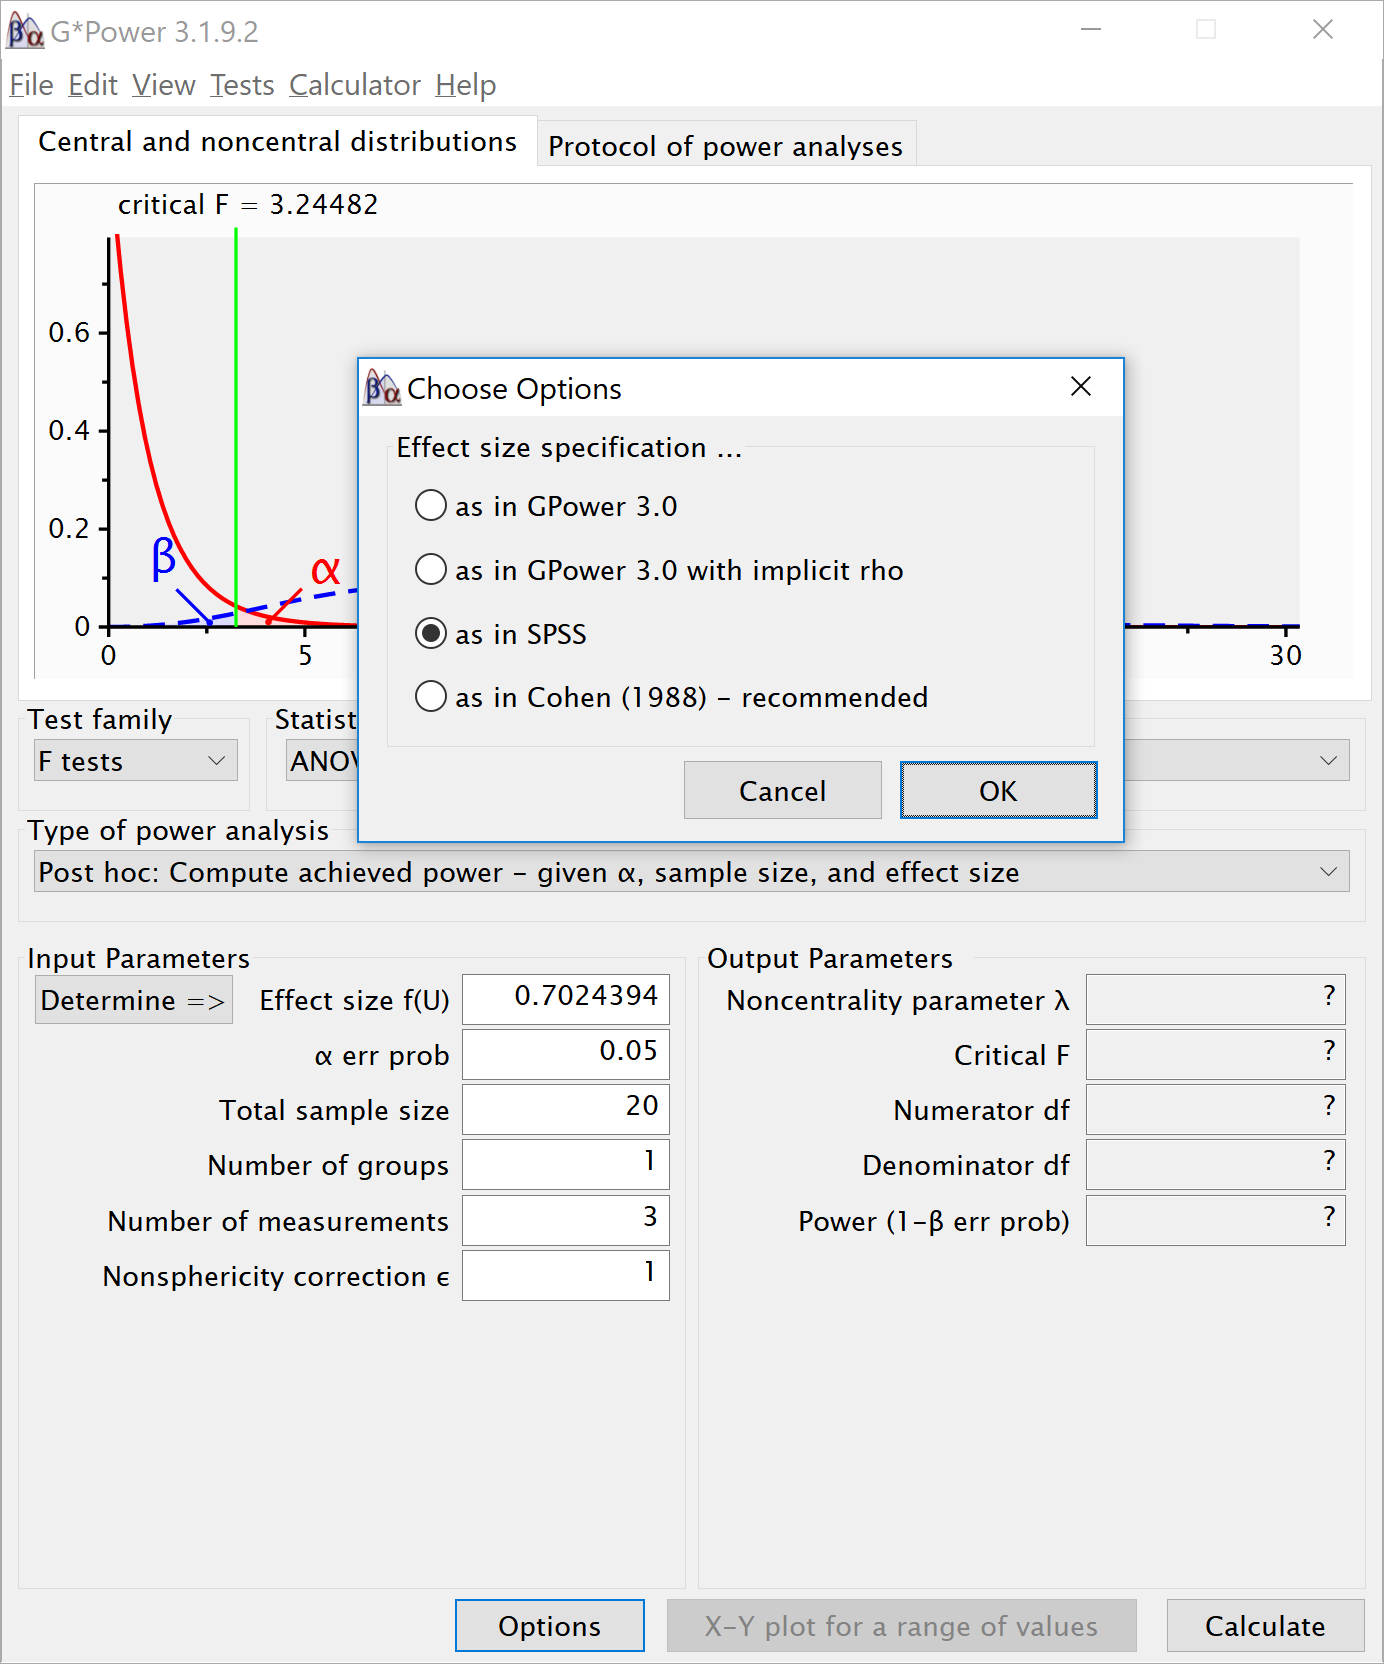
\includegraphics{screenshots/gpower_14.png}

\newpage

\hypertarget{part-3-1}{%
\section{Part 3}\label{part-3-1}}

We first repeat the simulation by Brysbaert:

\begin{Shaded}
\begin{Highlighting}[]
\CommentTok{# give sample size}
\NormalTok{N =}\StringTok{ }\DecValTok{75}
\CommentTok{# give effect size d}
\NormalTok{d1 =}\StringTok{ }\FloatTok{.4} \CommentTok{#difference between the extremes}
\NormalTok{d2 =}\StringTok{ }\FloatTok{.4} \CommentTok{#third condition goes with the highest extreme}
\CommentTok{# give the correlation between the conditions}
\NormalTok{r =}\StringTok{ }\FloatTok{.5}
\CommentTok{# give number of simulations}
\NormalTok{nSim =}\StringTok{ }\NormalTok{nsims}
\CommentTok{# give alpha levels}
\NormalTok{alpha1 =}\StringTok{ }\FloatTok{.05} \CommentTok{#alpha level for the omnibus ANOVA}
\NormalTok{alpha2 =}\StringTok{ }\FloatTok{.05} \CommentTok{#also adjusted from original by DL}
\end{Highlighting}
\end{Shaded}

\begin{Shaded}
\begin{Highlighting}[]
\CommentTok{# create vectors to store p-values}
\NormalTok{p1 <-}\StringTok{ }\KeywordTok{numeric}\NormalTok{(nSim) }\CommentTok{#p-value omnibus ANOVA}
\NormalTok{p2 <-}\StringTok{ }\KeywordTok{numeric}\NormalTok{(nSim) }\CommentTok{#p-value first post hoc test}
\NormalTok{p3 <-}\StringTok{ }\KeywordTok{numeric}\NormalTok{(nSim) }\CommentTok{#p-value second post hoc test}
\NormalTok{p4 <-}\StringTok{ }\KeywordTok{numeric}\NormalTok{(nSim) }\CommentTok{#p-value third post hoc test}

\CommentTok{# define correlation matrix}
\NormalTok{rho <-}\StringTok{ }\KeywordTok{cbind}\NormalTok{(}\KeywordTok{c}\NormalTok{(}\DecValTok{1}\NormalTok{, r, r), }\KeywordTok{c}\NormalTok{(r, }\DecValTok{1}\NormalTok{, r), }\KeywordTok{c}\NormalTok{(r, r, }\DecValTok{1}\NormalTok{))}
\CommentTok{# define participant codes}
\NormalTok{part <-}\StringTok{ }\KeywordTok{paste}\NormalTok{(}\StringTok{"part"}\NormalTok{,}\KeywordTok{seq}\NormalTok{(}\DecValTok{1}\OperatorTok{:}\NormalTok{N))}
\ControlFlowTok{for}\NormalTok{ (i }\ControlFlowTok{in} \DecValTok{1}\OperatorTok{:}\NormalTok{nSim) \{}
  \CommentTok{#for each simulated experiment}

\NormalTok{  data =}\StringTok{ }\KeywordTok{mvrnorm}\NormalTok{(}\DataTypeTok{n =}\NormalTok{ N,}
  \DataTypeTok{mu =} \KeywordTok{c}\NormalTok{(}\DecValTok{0}\NormalTok{, }\DecValTok{0}\NormalTok{, }\DecValTok{0}\NormalTok{),}
  \DataTypeTok{Sigma =}\NormalTok{ rho)}
\NormalTok{  data[, }\DecValTok{2}\NormalTok{] =}\StringTok{ }\NormalTok{data[, }\DecValTok{2}\NormalTok{] }\OperatorTok{+}\StringTok{ }\NormalTok{d1}
\NormalTok{  data[, }\DecValTok{3}\NormalTok{] =}\StringTok{ }\NormalTok{data[, }\DecValTok{3}\NormalTok{] }\OperatorTok{+}\StringTok{ }\NormalTok{d2}
\NormalTok{  datalong =}\StringTok{ }\KeywordTok{c}\NormalTok{(data[, }\DecValTok{1}\NormalTok{], data[, }\DecValTok{2}\NormalTok{], data[, }\DecValTok{3}\NormalTok{])}
\NormalTok{  conds =}\StringTok{ }\KeywordTok{factor}\NormalTok{(}\KeywordTok{rep}\NormalTok{(letters[}\DecValTok{24}\OperatorTok{:}\DecValTok{26}\NormalTok{], }\DataTypeTok{each =}\NormalTok{ N))}
\NormalTok{  partID =}\StringTok{ }\KeywordTok{factor}\NormalTok{(}\KeywordTok{rep}\NormalTok{(part, }\DataTypeTok{times =} \DecValTok{3}\NormalTok{))}
\NormalTok{  output <-}\StringTok{ }\KeywordTok{data.frame}\NormalTok{(partID, conds, datalong)}
\NormalTok{  test <-}\StringTok{ }\KeywordTok{aov}\NormalTok{(datalong }\OperatorTok{~}\StringTok{ }\NormalTok{conds }\OperatorTok{+}\StringTok{ }\KeywordTok{Error}\NormalTok{(partID }\OperatorTok{/}\StringTok{ }\NormalTok{conds), }\DataTypeTok{data =}\NormalTok{ output)}
\NormalTok{  tests <-}\StringTok{ }\NormalTok{(}\KeywordTok{summary}\NormalTok{(test))}
\NormalTok{  p1[i] <-}\StringTok{ }\NormalTok{tests}\OperatorTok{$}\StringTok{'Error: partID:conds'}\NormalTok{[[}\DecValTok{1}\NormalTok{]]}\OperatorTok{$}\StringTok{'Pr(>F)'}\NormalTok{[[}\DecValTok{1}\NormalTok{]]}
\NormalTok{  p2[i] <-}\StringTok{ }\KeywordTok{t.test}\NormalTok{(data[, }\DecValTok{1}\NormalTok{], data[, }\DecValTok{2}\NormalTok{], }\DataTypeTok{paired =} \OtherTok{TRUE}\NormalTok{)}\OperatorTok{$}\NormalTok{p.value}
\NormalTok{  p3[i] <-}\StringTok{ }\KeywordTok{t.test}\NormalTok{(data[, }\DecValTok{1}\NormalTok{], data[, }\DecValTok{3}\NormalTok{], }\DataTypeTok{paired =} \OtherTok{TRUE}\NormalTok{)}\OperatorTok{$}\NormalTok{p.value}
\NormalTok{  p4[i] <-}\StringTok{ }\KeywordTok{t.test}\NormalTok{(data[, }\DecValTok{2}\NormalTok{], data[, }\DecValTok{3}\NormalTok{], }\DataTypeTok{paired =} \OtherTok{TRUE}\NormalTok{)}\OperatorTok{$}\NormalTok{p.value}
\NormalTok{\}}
\end{Highlighting}
\end{Shaded}

\begin{Shaded}
\begin{Highlighting}[]
\CommentTok{#printing all unique tests (adjusted code by DL)}
\KeywordTok{sum}\NormalTok{(p1 }\OperatorTok{<}\StringTok{ }\NormalTok{alpha1) }\OperatorTok{/}\StringTok{ }\NormalTok{nSim}
\KeywordTok{sum}\NormalTok{(p2 }\OperatorTok{<}\StringTok{ }\NormalTok{alpha2) }\OperatorTok{/}\StringTok{ }\NormalTok{nSim}
\KeywordTok{sum}\NormalTok{(p3 }\OperatorTok{<}\StringTok{ }\NormalTok{alpha2) }\OperatorTok{/}\StringTok{ }\NormalTok{nSim}
\KeywordTok{sum}\NormalTok{(p4 }\OperatorTok{<}\StringTok{ }\NormalTok{alpha2) }\OperatorTok{/}\StringTok{ }\NormalTok{nSim}
\end{Highlighting}
\end{Shaded}

\begin{verbatim}
## [1] 0.7961
\end{verbatim}

\begin{verbatim}
## [1] 0.7624
\end{verbatim}

\begin{verbatim}
## [1] 0.7574
\end{verbatim}

\begin{verbatim}
## [1] 0.0452
\end{verbatim}

\hypertarget{reproducing-brysbaerts-examples}{%
\subsection{Reproducing Brysbaert's Examples}\label{reproducing-brysbaerts-examples}}

We can reproduce the same results as Brysbaert finds with his code:

\begin{Shaded}
\begin{Highlighting}[]
\NormalTok{design <-}\StringTok{ "3w"}
\NormalTok{n <-}\StringTok{ }\DecValTok{75}
\NormalTok{mu <-}\StringTok{ }\KeywordTok{c}\NormalTok{(}\DecValTok{0}\NormalTok{, }\FloatTok{0.4}\NormalTok{, }\FloatTok{0.4}\NormalTok{)}
\NormalTok{sd <-}\StringTok{ }\DecValTok{1}
\NormalTok{r <-}\StringTok{ }\FloatTok{0.5}
\NormalTok{labelnames <-}\StringTok{ }\KeywordTok{c}\NormalTok{(}\StringTok{"speed"}\NormalTok{, }\StringTok{"fast"}\NormalTok{, }\StringTok{"medium"}\NormalTok{, }\StringTok{"slow"}\NormalTok{)}
\end{Highlighting}
\end{Shaded}

We create the within design, and run the simulation

\begin{Shaded}
\begin{Highlighting}[]
\NormalTok{design_result <-}\StringTok{ }\KeywordTok{ANOVA_design}\NormalTok{(}\DataTypeTok{design =}\NormalTok{ design,}
                   \DataTypeTok{n =}\NormalTok{ n, }
                   \DataTypeTok{mu =}\NormalTok{ mu, }
                   \DataTypeTok{sd =}\NormalTok{ sd, }
                   \DataTypeTok{r =}\NormalTok{ r, }
                   \DataTypeTok{labelnames =}\NormalTok{ labelnames)}
\end{Highlighting}
\end{Shaded}

\begin{Shaded}
\begin{Highlighting}[]
\NormalTok{simulation_result <-}\StringTok{ }\KeywordTok{ANOVA_power}\NormalTok{(design_result, }
                                 \DataTypeTok{alpha_level =}\NormalTok{ alpha_level, }
                                 \DataTypeTok{nsims =}\NormalTok{ nsims,}
                                 \DataTypeTok{verbose =} \OtherTok{FALSE}\NormalTok{)}
\end{Highlighting}
\end{Shaded}

\begin{table}[!h]

\caption{\label{tab:unnamed-chunk-125}Simulated ANOVA Result}
\centering
\begin{tabular}{l|r|r}
\hline
  & power & effect\_size\\
\hline
anova\_speed & 95.25 & 0.1075912\\
\hline
\end{tabular}
\end{table}

\begin{Shaded}
\begin{Highlighting}[]
\NormalTok{exact_result <-}\StringTok{ }\KeywordTok{ANOVA_exact}\NormalTok{(design_result,}
                            \DataTypeTok{alpha_level =}\NormalTok{ alpha_level,}
                            \DataTypeTok{verbose =} \OtherTok{FALSE}\NormalTok{)}
\end{Highlighting}
\end{Shaded}

\begin{table}[!h]

\caption{\label{tab:unnamed-chunk-127}Exact ANOVA Result}
\centering
\begin{tabular}{l|r|r|r|r}
\hline
  & power & partial\_eta\_squared & cohen\_f & non\_centrality\\
\hline
speed & 95.29217 & 0.097561 & 0.328798 & 16\\
\hline
\end{tabular}
\end{table}

\textbf{Results}

The results of the simulation are very similar. Power for the ANOVA \emph{F}-test is around 95.2\%. For the three paired t-tests, power is around 92.7. This is in line with the a-priori power analysis when using Gpower:

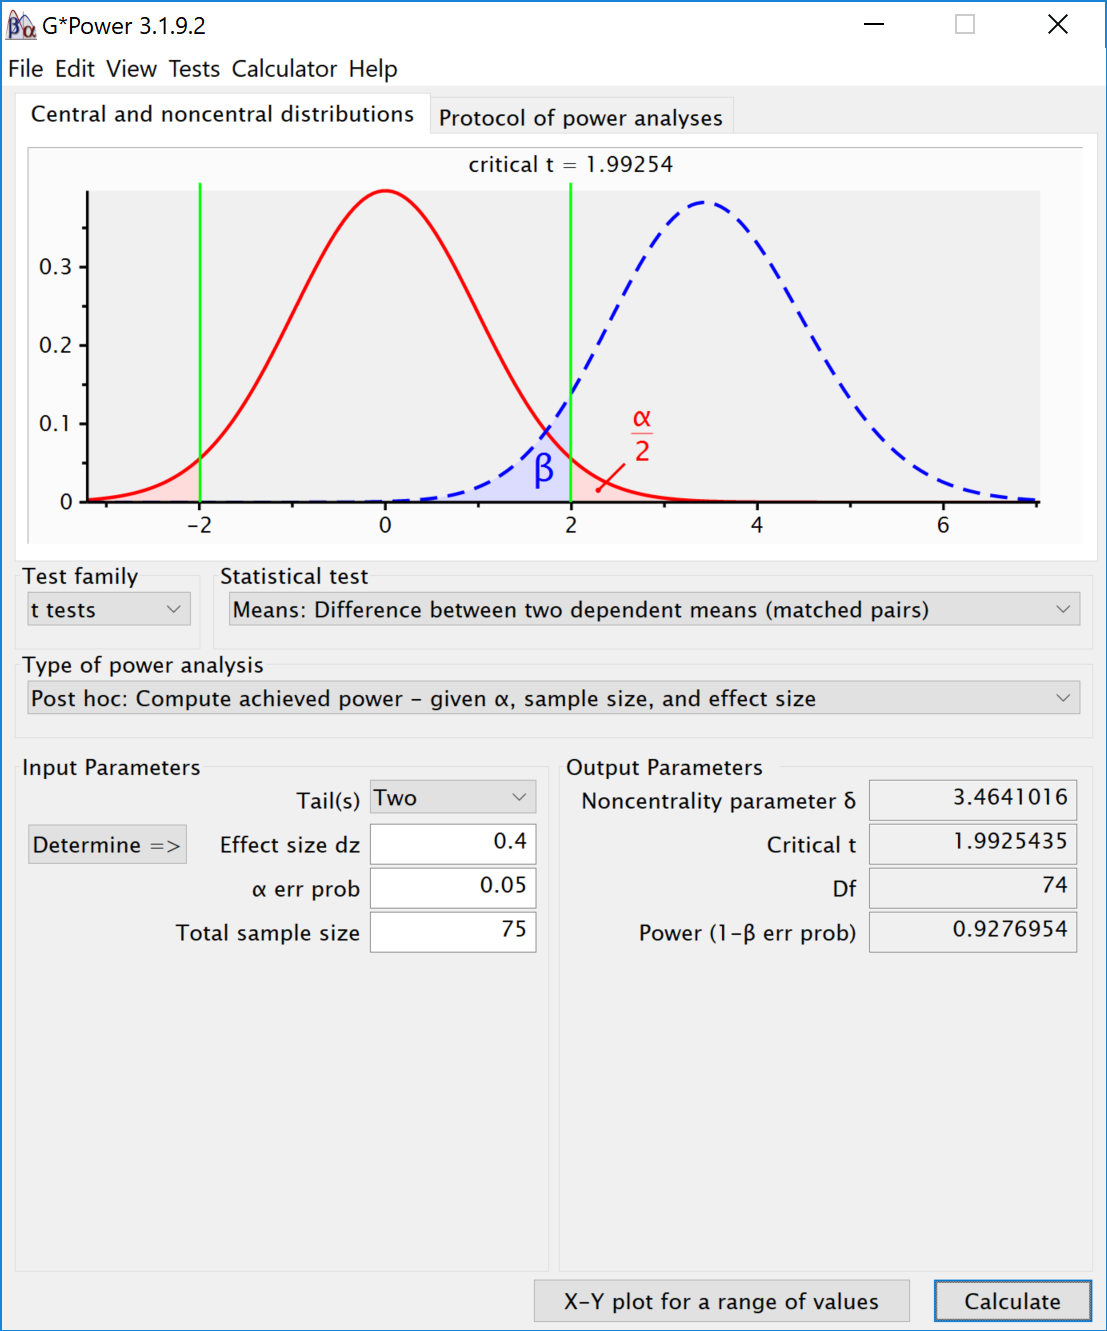
\includegraphics{screenshots/gpower_2.png}

We can perform an post-hoc power analysis in Gpower. We can calculate Cohen´s f based on the means and sd, using our own custom formula.

\begin{Shaded}
\begin{Highlighting}[]
\CommentTok{# Our simulation is based onthe following means and sd:}
\CommentTok{# mu <- c(0, 0.4, 0.4)}
\CommentTok{# sd <- 1}
\CommentTok{# Cohen, 1988, formula 8.2.1 and 8.2.2}
\NormalTok{f <-}\StringTok{ }\KeywordTok{sqrt}\NormalTok{(}\KeywordTok{sum}\NormalTok{((mu }\OperatorTok{-}\StringTok{ }\KeywordTok{mean}\NormalTok{(mu)) }\OperatorTok{^}\StringTok{ }\DecValTok{2}\NormalTok{) }\OperatorTok{/}\StringTok{ }\KeywordTok{length}\NormalTok{(mu)) }\OperatorTok{/}\StringTok{ }\NormalTok{sd }

\CommentTok{# We can see why f = 0.5*d.}
\CommentTok{# Imagine 2 group, mu = 1 and 2}
\CommentTok{# Grand mean is 1.5, }
\CommentTok{# we have sqrt(sum(0.5^2 + 0.5^2)/2), or sqrt(0.5/2), = 0.5.}
\CommentTok{# For Cohen's d we use the difference, 2-1 = 1. }
\end{Highlighting}
\end{Shaded}

The Cohen´s \emph{f} is 0.1885618. We can enter the \emph{f} (using the default 'as in G*Power 3.0' in the option window) and enter a sample size of 75, number of groups as 1, number of measurements as 3, correlation as 0.5. This yields:

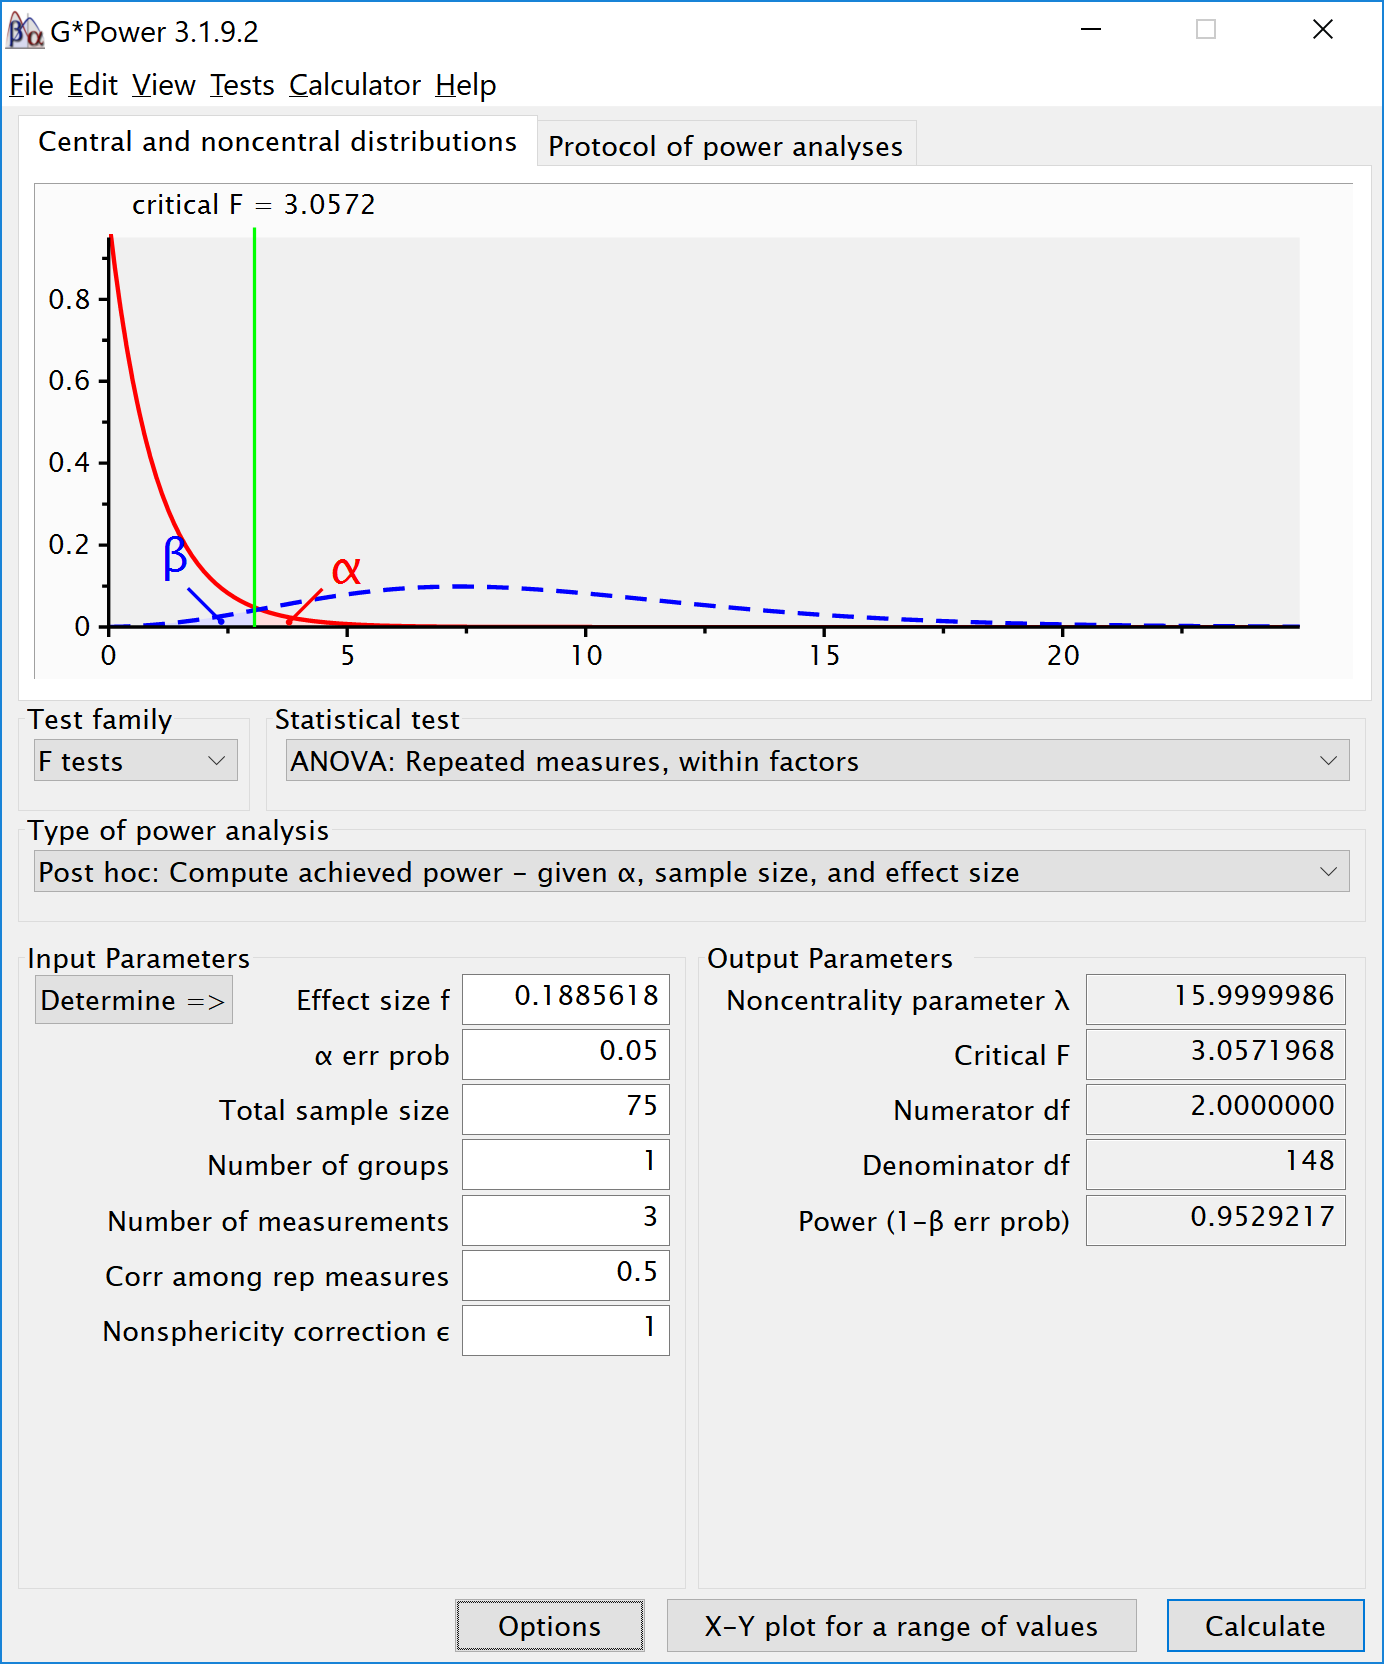
\includegraphics{screenshots/gpower_3.png}

\hypertarget{reproducing-brysbaert-variation-1-changing-correlation}{%
\subsection{Reproducing Brysbaert Variation 1: Changing Correlation}\label{reproducing-brysbaert-variation-1-changing-correlation}}

\begin{Shaded}
\begin{Highlighting}[]
\CommentTok{# give sample size}
\NormalTok{N =}\StringTok{ }\DecValTok{75}
\CommentTok{# give effect size d}
\NormalTok{d1 =}\StringTok{ }\FloatTok{.4} \CommentTok{#difference between the extremes}
\NormalTok{d2 =}\StringTok{ }\FloatTok{.4} \CommentTok{#third condition goes with the highest extreme}
\CommentTok{# give the correlation between the conditions}
\NormalTok{r =}\StringTok{ }\FloatTok{.6} \CommentTok{#increased correlation}
\CommentTok{# give number of simulations}
\NormalTok{nSim =}\StringTok{ }\NormalTok{nsims}
\CommentTok{# give alpha levels}
\NormalTok{alpha1 =}\StringTok{ }\FloatTok{.05} \CommentTok{#alpha level for the omnibus ANOVA}
\NormalTok{alpha2 =}\StringTok{ }\FloatTok{.05} \CommentTok{#also adjusted from original by DL}
\end{Highlighting}
\end{Shaded}

\begin{Shaded}
\begin{Highlighting}[]
\CommentTok{# create vectors to store p-values}
\NormalTok{p1 <-}\StringTok{ }\KeywordTok{numeric}\NormalTok{(nSim) }\CommentTok{#p-value omnibus ANOVA}
\NormalTok{p2 <-}\StringTok{ }\KeywordTok{numeric}\NormalTok{(nSim) }\CommentTok{#p-value first post hoc test}
\NormalTok{p3 <-}\StringTok{ }\KeywordTok{numeric}\NormalTok{(nSim) }\CommentTok{#p-value second post hoc test}
\NormalTok{p4 <-}\StringTok{ }\KeywordTok{numeric}\NormalTok{(nSim) }\CommentTok{#p-value third post hoc test}

\CommentTok{# define correlation matrix}
\NormalTok{rho <-}\StringTok{ }\KeywordTok{cbind}\NormalTok{(}\KeywordTok{c}\NormalTok{(}\DecValTok{1}\NormalTok{, r, r), }\KeywordTok{c}\NormalTok{(r, }\DecValTok{1}\NormalTok{, r), }\KeywordTok{c}\NormalTok{(r, r, }\DecValTok{1}\NormalTok{))}
\CommentTok{# define participant codes}
\NormalTok{part <-}\StringTok{ }\KeywordTok{paste}\NormalTok{(}\StringTok{"part"}\NormalTok{,}\KeywordTok{seq}\NormalTok{(}\DecValTok{1}\OperatorTok{:}\NormalTok{N))}
\ControlFlowTok{for}\NormalTok{ (i }\ControlFlowTok{in} \DecValTok{1}\OperatorTok{:}\NormalTok{nSim) \{}
  
  \CommentTok{#for each simulated experiment}

\NormalTok{  data =}\StringTok{ }\KeywordTok{mvrnorm}\NormalTok{(}\DataTypeTok{n =}\NormalTok{ N,}
  \DataTypeTok{mu =} \KeywordTok{c}\NormalTok{(}\DecValTok{0}\NormalTok{, }\DecValTok{0}\NormalTok{, }\DecValTok{0}\NormalTok{),}
  \DataTypeTok{Sigma =}\NormalTok{ rho)}
\NormalTok{  data[, }\DecValTok{2}\NormalTok{] =}\StringTok{ }\NormalTok{data[, }\DecValTok{2}\NormalTok{] }\OperatorTok{+}\StringTok{ }\NormalTok{d1}
\NormalTok{  data[, }\DecValTok{3}\NormalTok{] =}\StringTok{ }\NormalTok{data[, }\DecValTok{3}\NormalTok{] }\OperatorTok{+}\StringTok{ }\NormalTok{d2}
\NormalTok{  datalong =}\StringTok{ }\KeywordTok{c}\NormalTok{(data[, }\DecValTok{1}\NormalTok{], data[, }\DecValTok{2}\NormalTok{], data[, }\DecValTok{3}\NormalTok{])}
\NormalTok{  conds =}\StringTok{ }\KeywordTok{factor}\NormalTok{(}\KeywordTok{rep}\NormalTok{(letters[}\DecValTok{24}\OperatorTok{:}\DecValTok{26}\NormalTok{], }\DataTypeTok{each =}\NormalTok{ N))}
\NormalTok{  partID =}\StringTok{ }\KeywordTok{factor}\NormalTok{(}\KeywordTok{rep}\NormalTok{(part, }\DataTypeTok{times =} \DecValTok{3}\NormalTok{))}
\NormalTok{  output <-}\StringTok{ }\KeywordTok{data.frame}\NormalTok{(partID, conds, datalong)}
\NormalTok{  test <-}\StringTok{ }\KeywordTok{aov}\NormalTok{(datalong }\OperatorTok{~}\StringTok{ }\NormalTok{conds }\OperatorTok{+}\StringTok{ }\KeywordTok{Error}\NormalTok{(partID }\OperatorTok{/}\StringTok{ }\NormalTok{conds), }
              \DataTypeTok{data =}\NormalTok{ output)}
\NormalTok{  tests <-}\StringTok{ }\NormalTok{(}\KeywordTok{summary}\NormalTok{(test))}
\NormalTok{  p1[i] <-}\StringTok{ }\NormalTok{tests}\OperatorTok{$}\StringTok{'Error: partID:conds'}\NormalTok{[[}\DecValTok{1}\NormalTok{]]}\OperatorTok{$}\StringTok{'Pr(>F)'}\NormalTok{[[}\DecValTok{1}\NormalTok{]]}
\NormalTok{  p2[i] <-}\StringTok{ }\KeywordTok{t.test}\NormalTok{(data[, }\DecValTok{1}\NormalTok{], data[, }\DecValTok{2}\NormalTok{], }\DataTypeTok{paired =} \OtherTok{TRUE}\NormalTok{)}\OperatorTok{$}\NormalTok{p.value}
\NormalTok{  p3[i] <-}\StringTok{ }\KeywordTok{t.test}\NormalTok{(data[, }\DecValTok{1}\NormalTok{], data[, }\DecValTok{3}\NormalTok{], }\DataTypeTok{paired =} \OtherTok{TRUE}\NormalTok{)}\OperatorTok{$}\NormalTok{p.value}
\NormalTok{  p4[i] <-}\StringTok{ }\KeywordTok{t.test}\NormalTok{(data[, }\DecValTok{2}\NormalTok{], data[, }\DecValTok{3}\NormalTok{], }\DataTypeTok{paired =} \OtherTok{TRUE}\NormalTok{)}\OperatorTok{$}\NormalTok{p.value}
\NormalTok{\}}
\end{Highlighting}
\end{Shaded}

\begin{Shaded}
\begin{Highlighting}[]
\KeywordTok{sum}\NormalTok{(p1 }\OperatorTok{<}\StringTok{ }\NormalTok{alpha1) }\OperatorTok{/}\StringTok{ }\NormalTok{nSim}
\KeywordTok{sum}\NormalTok{(p2 }\OperatorTok{<}\StringTok{ }\NormalTok{alpha2) }\OperatorTok{/}\StringTok{ }\NormalTok{nSim}
\KeywordTok{sum}\NormalTok{(p3 }\OperatorTok{<}\StringTok{ }\NormalTok{alpha2) }\OperatorTok{/}\StringTok{ }\NormalTok{nSim}
\KeywordTok{sum}\NormalTok{(p4 }\OperatorTok{<}\StringTok{ }\NormalTok{alpha2) }\OperatorTok{/}\StringTok{ }\NormalTok{nSim}
\end{Highlighting}
\end{Shaded}

\begin{verbatim}
## [1] 0.9472
\end{verbatim}

\begin{verbatim}
## [1] 0.9245
\end{verbatim}

\begin{verbatim}
## [1] 0.0503
\end{verbatim}

\begin{verbatim}
## [1] 0.923
\end{verbatim}

\begin{Shaded}
\begin{Highlighting}[]
\NormalTok{design <-}\StringTok{ "3w"}
\NormalTok{n <-}\StringTok{ }\DecValTok{75}
\NormalTok{mu <-}\StringTok{ }\KeywordTok{c}\NormalTok{(}\DecValTok{0}\NormalTok{, }\FloatTok{0.4}\NormalTok{, }\FloatTok{0.4}\NormalTok{)}
\NormalTok{sd <-}\StringTok{ }\DecValTok{1}
\NormalTok{r <-}\StringTok{ }\FloatTok{0.6}
\NormalTok{labelnames <-}\StringTok{ }\KeywordTok{c}\NormalTok{(}\StringTok{"SPEED"}\NormalTok{, }
                \StringTok{"fast"}\NormalTok{, }\StringTok{"medium"}\NormalTok{, }\StringTok{"slow"}\NormalTok{)}
\end{Highlighting}
\end{Shaded}

We create the 3-level repeated measures design, and run the simulation.

\begin{Shaded}
\begin{Highlighting}[]
\NormalTok{design_result <-}\StringTok{ }\KeywordTok{ANOVA_design}\NormalTok{(}\DataTypeTok{design =}\NormalTok{ design,}
                   \DataTypeTok{n =}\NormalTok{ n, }
                   \DataTypeTok{mu =}\NormalTok{ mu, }
                   \DataTypeTok{sd =}\NormalTok{ sd, }
                   \DataTypeTok{r =}\NormalTok{ r, }
                   \DataTypeTok{labelnames =}\NormalTok{ labelnames)}
\end{Highlighting}
\end{Shaded}

\begin{Shaded}
\begin{Highlighting}[]
\NormalTok{simulation_result <-}\StringTok{ }\KeywordTok{ANOVA_power}\NormalTok{(design_result, }
                                 \DataTypeTok{alpha_level =}\NormalTok{ alpha_level, }
                                 \DataTypeTok{nsims =}\NormalTok{ nsims,}
                                 \DataTypeTok{verbose =} \OtherTok{FALSE}\NormalTok{)}
\end{Highlighting}
\end{Shaded}

\begin{table}[!h]

\caption{\label{tab:unnamed-chunk-136}Simulated ANOVA Result}
\centering
\begin{tabular}{l|r|r}
\hline
  & power & effect\_size\\
\hline
anova\_SPEED & 98.37 & 0.1287432\\
\hline
\end{tabular}
\end{table}

\begin{Shaded}
\begin{Highlighting}[]
\NormalTok{exact_result <-}\StringTok{ }\KeywordTok{ANOVA_exact}\NormalTok{(design_result,}
                            \DataTypeTok{alpha_level =}\NormalTok{ alpha_level,}
                            \DataTypeTok{verbose =} \OtherTok{FALSE}\NormalTok{)}
\end{Highlighting}
\end{Shaded}

\begin{table}[!h]

\caption{\label{tab:unnamed-chunk-138}Exact ANOVA Result}
\centering
\begin{tabular}{l|r|r|r|r}
\hline
  & power & partial\_eta\_squared & cohen\_f & non\_centrality\\
\hline
SPEED & 98.34682 & 0.1190476 & 0.3676073 & 20\\
\hline
\end{tabular}
\end{table}

Again, this is similar to GPower for the ANOVA:

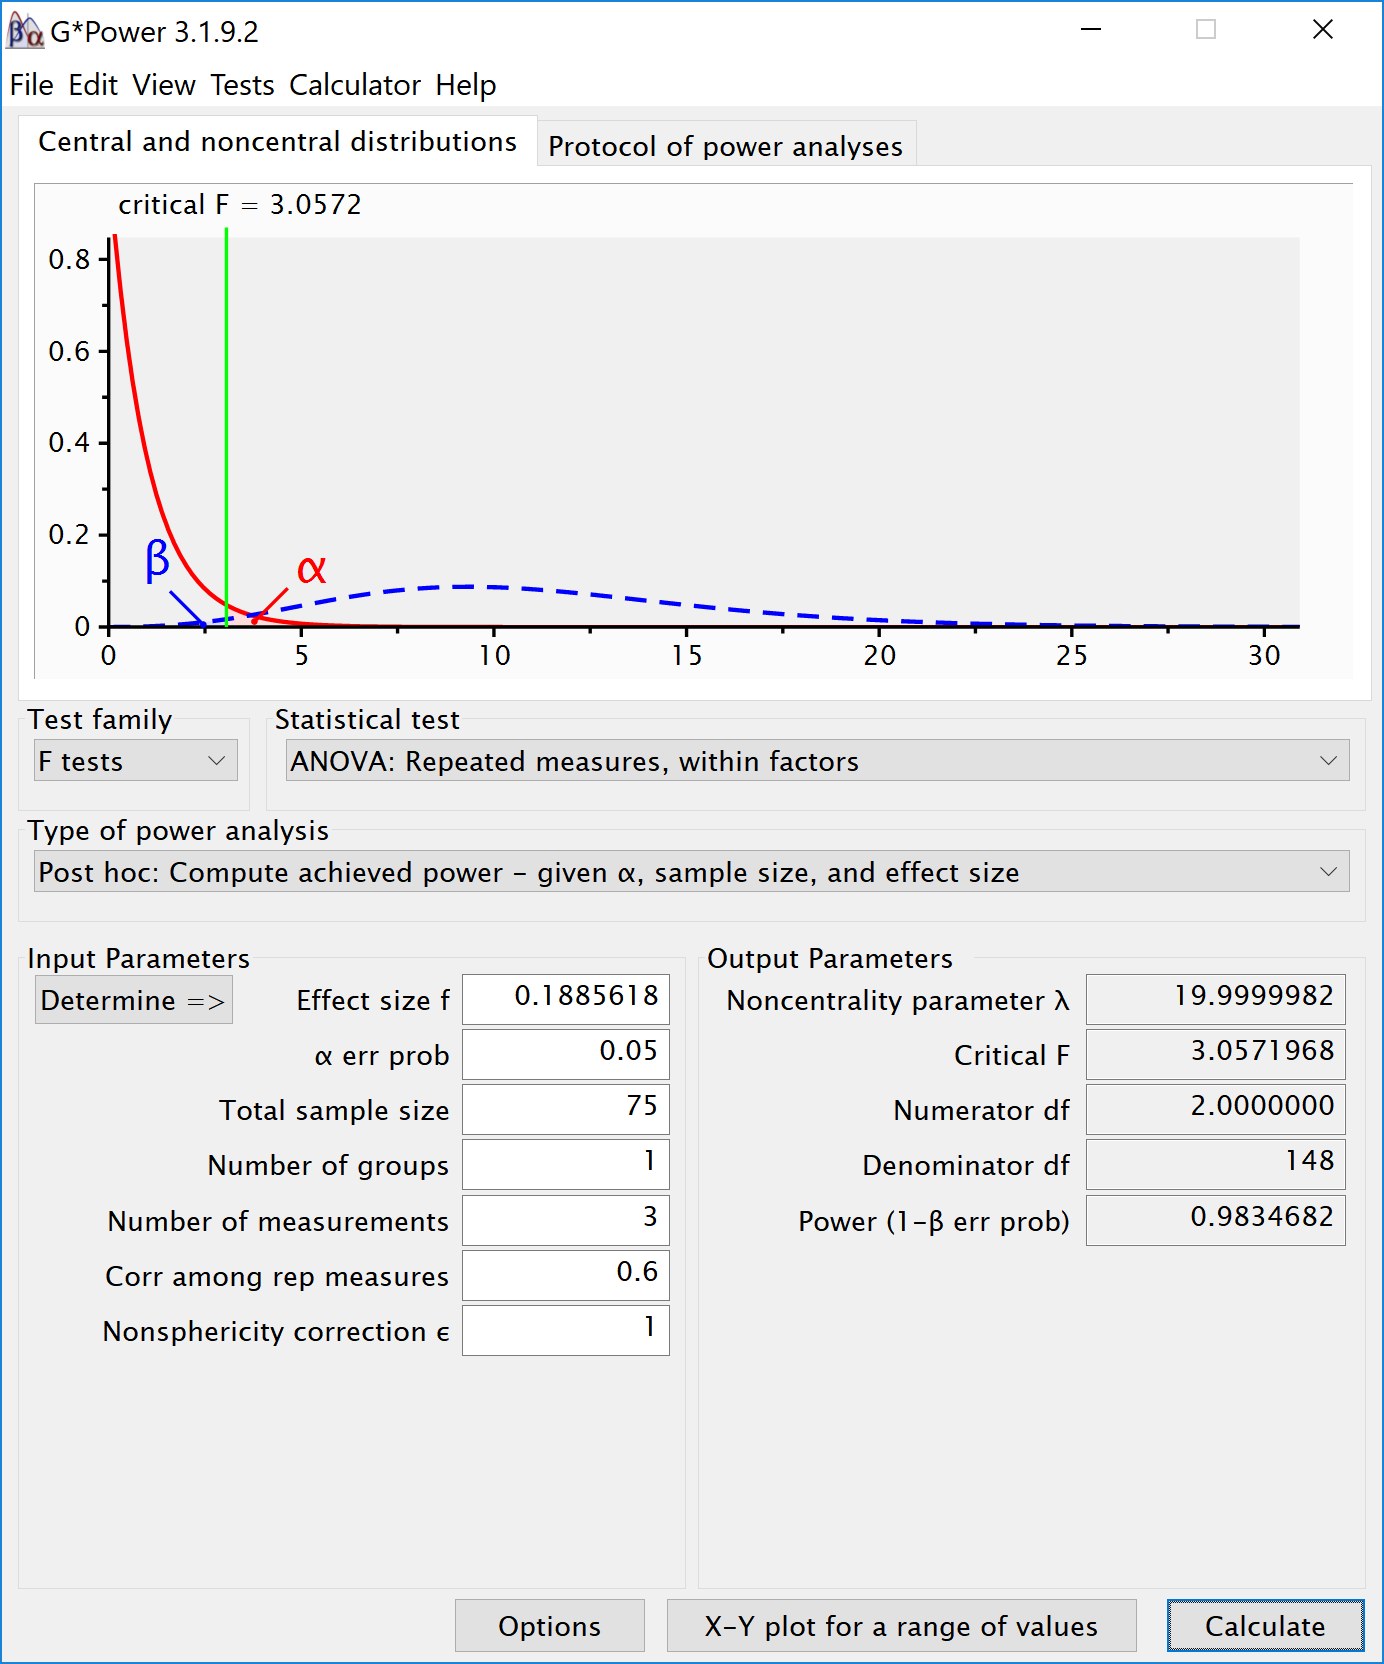
\includegraphics{screenshots/gpower_4.png}

\newpage

\hypertarget{part-4}{%
\section{Part 4}\label{part-4}}

\hypertarget{x2-anova-within-within-design}{%
\subsection{2x2 ANOVA, within-within design}\label{x2-anova-within-within-design}}

We can simulate a 2x2 ANOVA, both factors manipulated within participants, with a specific sample size and effect size, to achieve a desired statistical power.

As \citet{potvin2000statistical} explain, analytic procedures for a two-factor repeated measures ANOVA do not seem to exist. The main problem is quantifying the error variance (the denominator when calculating lambda or Cohen's \emph{f}). Simulation based aproaches provide a solution.

We can reproduce the simulation coded by \href{https://cognitivedatascientist.com/2015/12/14/power-simulation-in-r-the-repeated-measures-anova-5/}{Ben Amsel}

\begin{Shaded}
\begin{Highlighting}[]
\CommentTok{# define the parameters}
\CommentTok{# true effects (in this case, a double dissociation)}
\NormalTok{mu =}\StringTok{ }\KeywordTok{c}\NormalTok{(}\DecValTok{700}\NormalTok{, }\DecValTok{670}\NormalTok{, }\DecValTok{670}\NormalTok{, }\DecValTok{700}\NormalTok{) }
\NormalTok{sigma =}\StringTok{ }\DecValTok{150}  \CommentTok{# population standard deviation}
\NormalTok{rho =}\StringTok{ }\FloatTok{0.75} \CommentTok{# correlation between repeated measures}
\NormalTok{nsubs =}\StringTok{ }\DecValTok{25} \CommentTok{# how many subjects?}
\NormalTok{nsims =}\StringTok{ }\NormalTok{nsims }\CommentTok{# how many simulation replicates?}
 
\CommentTok{# create 2 factors representing the 2 independent variables}
\NormalTok{cond =}\StringTok{ }\KeywordTok{data.frame}\NormalTok{(}\DataTypeTok{X1 =} \KeywordTok{rep}\NormalTok{(}\KeywordTok{factor}\NormalTok{(letters[}\DecValTok{1}\OperatorTok{:}\DecValTok{2}\NormalTok{]), nsubs }\OperatorTok{*}\StringTok{ }\DecValTok{2}\NormalTok{),}
                  \DataTypeTok{X2 =} \KeywordTok{rep}\NormalTok{(}\KeywordTok{factor}\NormalTok{(letters[}\DecValTok{1}\OperatorTok{:}\DecValTok{2}\NormalTok{]), nsubs, }\DataTypeTok{each =} \DecValTok{2}\NormalTok{))}
 
\CommentTok{# create a subjects factor}
\NormalTok{subject =}\StringTok{ }\KeywordTok{factor}\NormalTok{(}\KeywordTok{sort}\NormalTok{(}\KeywordTok{rep}\NormalTok{(}\DecValTok{1}\OperatorTok{:}\NormalTok{nsubs, }\DecValTok{4}\NormalTok{)))}
 
\CommentTok{# combine above into the design matrix}
\NormalTok{dm =}\StringTok{ }\KeywordTok{data.frame}\NormalTok{(subject, cond)}
\end{Highlighting}
\end{Shaded}

Build Sigma: the population variance-covariance matrix

\begin{Shaded}
\begin{Highlighting}[]
\CommentTok{# create k x k matrix populated with sigma}
\NormalTok{sigma.mat <-}\StringTok{ }\KeywordTok{rep}\NormalTok{(sigma, }\DecValTok{4}\NormalTok{)}
\NormalTok{S <-}
\StringTok{  }\KeywordTok{matrix}\NormalTok{(sigma.mat,}
  \DataTypeTok{ncol =} \KeywordTok{length}\NormalTok{(sigma.mat),}
  \DataTypeTok{nrow =} \KeywordTok{length}\NormalTok{(sigma.mat))}
 
\CommentTok{# compute covariance between measures}
\NormalTok{Sigma <-}\StringTok{ }\KeywordTok{t}\NormalTok{(S) }\OperatorTok{*}\StringTok{ }\NormalTok{S }\OperatorTok{*}\StringTok{ }\NormalTok{rho  }
 
\CommentTok{# put the variances on the diagonal }
\KeywordTok{diag}\NormalTok{(Sigma) <-}\StringTok{ }\NormalTok{sigma}\OperatorTok{^}\DecValTok{2}  
\end{Highlighting}
\end{Shaded}

Run the simulation

\begin{Shaded}
\begin{Highlighting}[]
\CommentTok{# stack 'nsims' individual data frames into one large data frame}
\NormalTok{df =}\StringTok{ }\NormalTok{dm[}\KeywordTok{rep}\NormalTok{(}\KeywordTok{seq_len}\NormalTok{(}\KeywordTok{nrow}\NormalTok{(dm)), nsims), ]}
 
\CommentTok{# add an index column to track the simulation run}
\NormalTok{df}\OperatorTok{$}\NormalTok{simID =}\StringTok{ }\KeywordTok{sort}\NormalTok{(}\KeywordTok{rep}\NormalTok{(}\KeywordTok{seq_len}\NormalTok{(nsims), }\KeywordTok{nrow}\NormalTok{(dm)))}
 
\CommentTok{# sample the observed data from a multivariate normal distribution}
\CommentTok{# using MASS::mvrnorm with the mu and Sigma created earlier}
\CommentTok{# and bind to the existing df}
 

\NormalTok{make.y =}\StringTok{ }\KeywordTok{expression}\NormalTok{(}\KeywordTok{as.vector}\NormalTok{(}\KeywordTok{t}\NormalTok{(}\KeywordTok{mvrnorm}\NormalTok{(nsubs, mu, Sigma))))}
\NormalTok{df}\OperatorTok{$}\NormalTok{y =}\StringTok{ }\KeywordTok{as.vector}\NormalTok{(}\KeywordTok{replicate}\NormalTok{(nsims, }\KeywordTok{eval}\NormalTok{(make.y)))             }
 
\CommentTok{# use do(), the general purpose complement to the specialized data }
\CommentTok{# manipulation functions available in dplyr, to run the ANOVA on}
\CommentTok{# each section of the grouped data frame created by group_by}
 

\NormalTok{mods <-}\StringTok{ }\NormalTok{df }\OperatorTok
\StringTok{  }\KeywordTok{group_by}\NormalTok{(simID) }\OperatorTok
\StringTok{  }\KeywordTok{do}\NormalTok{(}\DataTypeTok{model =} \KeywordTok{aov}\NormalTok{(y }\OperatorTok{~}\StringTok{ }\NormalTok{X1 }\OperatorTok{*}\StringTok{ }\NormalTok{X2 }\OperatorTok{+}\StringTok{ }\KeywordTok{Error}\NormalTok{(subject }\OperatorTok{/}\StringTok{ }\NormalTok{(X1 }\OperatorTok{*}\StringTok{ }\NormalTok{X2)), }
                 \DataTypeTok{qr =} \OtherTok{FALSE}\NormalTok{, }\DataTypeTok{data =}\NormalTok{ .)) }
 
\CommentTok{# extract p-values for each effect and store in a data frame}
\NormalTok{p_val_}\DecValTok{1}\NormalTok{ =}\StringTok{ }\KeywordTok{data.frame}\NormalTok{(}
\NormalTok{  mods }\OperatorTok\StringTok{ }\KeywordTok{do}\NormalTok{(}\KeywordTok{as.data.frame}\NormalTok{(}\KeywordTok{tidy}\NormalTok{(.}\OperatorTok{$}\NormalTok{model[[}\DecValTok{3}\NormalTok{]])}\OperatorTok{$}\NormalTok{p.value[}\DecValTok{1}\NormalTok{])),}
\NormalTok{  mods }\OperatorTok\StringTok{ }\KeywordTok{do}\NormalTok{(}\KeywordTok{as.data.frame}\NormalTok{(}\KeywordTok{tidy}\NormalTok{(.}\OperatorTok{$}\NormalTok{model[[}\DecValTok{4}\NormalTok{]])}\OperatorTok{$}\NormalTok{p.value[}\DecValTok{1}\NormalTok{])),}
\NormalTok{  mods }\OperatorTok\StringTok{ }\KeywordTok{do}\NormalTok{(}\KeywordTok{as.data.frame}\NormalTok{(}\KeywordTok{tidy}\NormalTok{(.}\OperatorTok{$}\NormalTok{model[[}\DecValTok{5}\NormalTok{]])}\OperatorTok{$}\NormalTok{p.value[}\DecValTok{1}\NormalTok{])))}
\KeywordTok{colnames}\NormalTok{(p_val_}\DecValTok{1}\NormalTok{) =}\StringTok{ }\KeywordTok{c}\NormalTok{(}\StringTok{'X1'}\NormalTok{,}\StringTok{'X2'}\NormalTok{,}\StringTok{'Interaction'}\NormalTok{)}
\end{Highlighting}
\end{Shaded}

The empirical power is easy to compute, it's just the proportion of simulation runs where \emph{p} \textless{} .05.

\begin{Shaded}
\begin{Highlighting}[]
\NormalTok{power.res =}\StringTok{ }\KeywordTok{apply}\NormalTok{(}\KeywordTok{as.matrix}\NormalTok{(p_val_}\DecValTok{1}\NormalTok{), }\DecValTok{2}\NormalTok{, }
  \ControlFlowTok{function}\NormalTok{(x) }\KeywordTok{round}\NormalTok{(}\KeywordTok{mean}\NormalTok{(}\KeywordTok{ifelse}\NormalTok{(x }\OperatorTok{<}\StringTok{ }\FloatTok{.05}\NormalTok{, }\DecValTok{1}\NormalTok{, }\DecValTok{0}\NormalTok{) }\OperatorTok{*}\StringTok{ }\DecValTok{100}\NormalTok{),}\DecValTok{2}\NormalTok{))}
\NormalTok{power.res}
\end{Highlighting}
\end{Shaded}

\begin{verbatim}
##          X1          X2 Interaction 
##        4.80        4.66       47.50
\end{verbatim}

Visualize the distributions of \emph{p}-values

\begin{Shaded}
\begin{Highlighting}[]
\CommentTok{# plot the known effects}

 
\NormalTok{means =}\StringTok{ }\KeywordTok{data.frame}\NormalTok{(cond[}\DecValTok{1}\OperatorTok{:}\DecValTok{4}\NormalTok{,], mu, }\DataTypeTok{SE =}\NormalTok{ sigma }\OperatorTok{/}\StringTok{ }\KeywordTok{sqrt}\NormalTok{(nsubs))}
\NormalTok{plt1 =}\StringTok{ }\KeywordTok{ggplot}\NormalTok{(means, }\KeywordTok{aes}\NormalTok{(}\DataTypeTok{y =}\NormalTok{ mu, }\DataTypeTok{x =}\NormalTok{ X1, }\DataTypeTok{fill =}\NormalTok{ X2)) }\OperatorTok{+}
\KeywordTok{geom_bar}\NormalTok{(}\DataTypeTok{position =} \KeywordTok{position_dodge}\NormalTok{(), }\DataTypeTok{stat =} \StringTok{"identity"}\NormalTok{) }\OperatorTok{+}
\KeywordTok{geom_errorbar}\NormalTok{(}
\KeywordTok{aes}\NormalTok{(}\DataTypeTok{ymin =}\NormalTok{ mu }\OperatorTok{-}\StringTok{ }\NormalTok{SE, }\DataTypeTok{ymax =}\NormalTok{ mu }\OperatorTok{+}\StringTok{ }\NormalTok{SE),}
\DataTypeTok{position =} \KeywordTok{position_dodge}\NormalTok{(}\DataTypeTok{width =} \FloatTok{0.9}\NormalTok{),}
\DataTypeTok{size =} \FloatTok{.6}\NormalTok{,}
\DataTypeTok{width =} \FloatTok{.3}
\NormalTok{) }\OperatorTok{+}
\KeywordTok{coord_cartesian}\NormalTok{(}\DataTypeTok{ylim =} \KeywordTok{c}\NormalTok{((.}\DecValTok{7} \OperatorTok{*}\StringTok{ }\KeywordTok{min}\NormalTok{(mu)), }\FloatTok{1.2} \OperatorTok{*}\StringTok{ }\KeywordTok{max}\NormalTok{(mu))) }\OperatorTok{+}
\KeywordTok{theme_bw}\NormalTok{()}

\CommentTok{# melt the data into a ggplot friendly 'long' format}

\NormalTok{plotData <-}\StringTok{ }\KeywordTok{melt}\NormalTok{(p_val_}\DecValTok{1}\NormalTok{, }\DataTypeTok{value.name =} \StringTok{'p'}\NormalTok{)}

\CommentTok{# plot each of the p-value distributions on a log scale}
\KeywordTok{options}\NormalTok{(}\DataTypeTok{scipen =} \DecValTok{999}\NormalTok{) }\CommentTok{# 'turn off' scientific notation}
\NormalTok{plt2 =}\StringTok{ }\KeywordTok{ggplot}\NormalTok{(plotData, }\KeywordTok{aes}\NormalTok{(}\DataTypeTok{x =}\NormalTok{ p)) }\OperatorTok{+}
\KeywordTok{scale_x_log10}\NormalTok{(}\DataTypeTok{breaks =} \KeywordTok{c}\NormalTok{(}\DecValTok{1}\NormalTok{, }\FloatTok{0.05}\NormalTok{, }\FloatTok{0.001}\NormalTok{),}
\DataTypeTok{labels =} \KeywordTok{c}\NormalTok{(}\DecValTok{1}\NormalTok{, }\FloatTok{0.05}\NormalTok{, }\FloatTok{0.001}\NormalTok{)) }\OperatorTok{+}
\KeywordTok{geom_histogram}\NormalTok{(}\DataTypeTok{colour =} \StringTok{"darkblue"}\NormalTok{, }\DataTypeTok{fill =} \StringTok{"white"}\NormalTok{) }\OperatorTok{+}
\KeywordTok{geom_vline}\NormalTok{(}\DataTypeTok{xintercept =} \FloatTok{0.05}\NormalTok{, }\DataTypeTok{colour =} \StringTok{'red'}\NormalTok{) }\OperatorTok{+}
\KeywordTok{facet_grid}\NormalTok{(variable }\OperatorTok{~}\StringTok{ }\NormalTok{.) }\OperatorTok{+}
\KeywordTok{labs}\NormalTok{(}\DataTypeTok{x =} \KeywordTok{expression}\NormalTok{(Log[}\DecValTok{10}\NormalTok{] }\OperatorTok{~}\StringTok{ }\NormalTok{P)) }\OperatorTok{+}
\KeywordTok{theme}\NormalTok{(}\DataTypeTok{axis.text.x =} \KeywordTok{element_text}\NormalTok{(}\DataTypeTok{color =} \StringTok{'black'}\NormalTok{, }\DataTypeTok{size =} \DecValTok{7}\NormalTok{))}

\CommentTok{# arrange plots side by side and print}
\KeywordTok{grid.arrange}\NormalTok{(plt1, plt2, }\DataTypeTok{nrow =} \DecValTok{1}\NormalTok{)}
\end{Highlighting}
\end{Shaded}

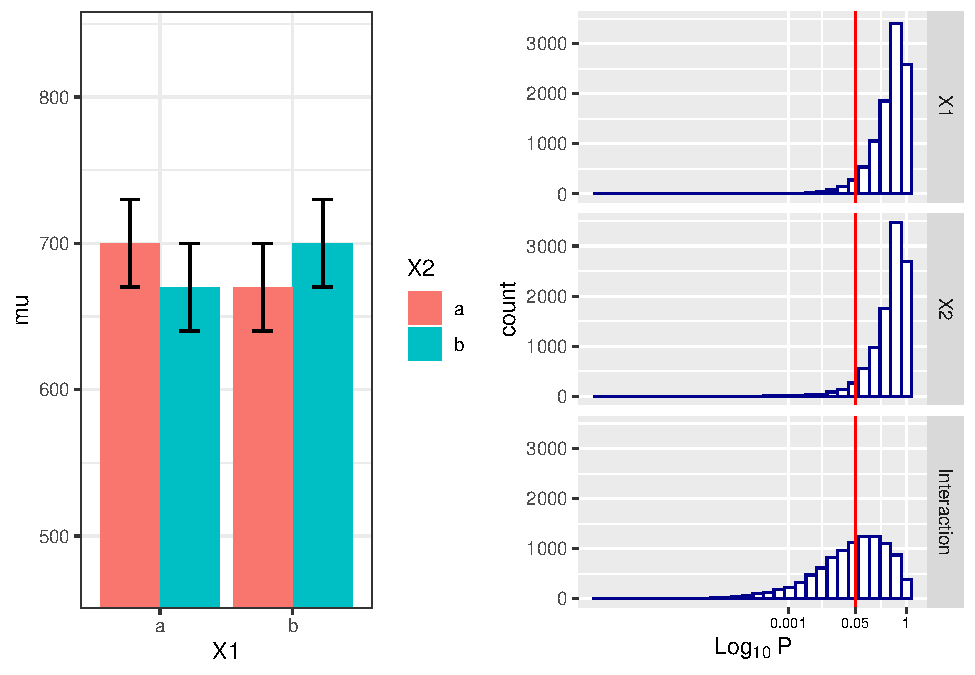
\includegraphics{SuperpowerValidation_files/figure-latex/unnamed-chunk-144-1.pdf}

We can reproduce this simulation:

\begin{Shaded}
\begin{Highlighting}[]
\CommentTok{# true effects (in this case, a double dissociation)}
\NormalTok{mu =}\StringTok{ }\KeywordTok{c}\NormalTok{(}\DecValTok{700}\NormalTok{, }\DecValTok{670}\NormalTok{, }\DecValTok{670}\NormalTok{, }\DecValTok{700}\NormalTok{) }
\NormalTok{sigma =}\StringTok{ }\DecValTok{150}  \CommentTok{# population standard deviation}
\NormalTok{n <-}\StringTok{ }\DecValTok{25}
\NormalTok{sd <-}\StringTok{ }\DecValTok{150}
\NormalTok{r <-}\StringTok{ }\FloatTok{0.75}
\NormalTok{string =}\StringTok{ "2w*2w"}
\NormalTok{alpha_level <-}\StringTok{ }\FloatTok{0.05}
\NormalTok{labelnames =}\StringTok{ }\KeywordTok{c}\NormalTok{(}\StringTok{"age"}\NormalTok{, }\StringTok{"old"}\NormalTok{, }\StringTok{"young"}\NormalTok{, }\StringTok{"color"}\NormalTok{, }\StringTok{"blue"}\NormalTok{, }\StringTok{"red"}\NormalTok{)}
\NormalTok{design_result <-}\StringTok{ }\KeywordTok{ANOVA_design}\NormalTok{(}\DataTypeTok{design =}\NormalTok{ string,}
                              \DataTypeTok{n =}\NormalTok{ n, }
                              \DataTypeTok{mu =}\NormalTok{ mu, }
                              \DataTypeTok{sd =}\NormalTok{ sd, }
                              \DataTypeTok{r =}\NormalTok{ r, }
                              \DataTypeTok{labelnames =}\NormalTok{ labelnames)}
\end{Highlighting}
\end{Shaded}

\begin{Shaded}
\begin{Highlighting}[]
\NormalTok{simulation_result <-}\StringTok{ }\KeywordTok{ANOVA_power}\NormalTok{(design_result, }
                                 \DataTypeTok{alpha_level =}\NormalTok{ alpha_level, }
                                 \DataTypeTok{nsims =}\NormalTok{ nsims,}
                                 \DataTypeTok{verbose =} \OtherTok{FALSE}\NormalTok{)}
\end{Highlighting}
\end{Shaded}

\begin{table}[!h]

\caption{\label{tab:unnamed-chunk-147}Simulated ANOVA Result}
\centering
\begin{tabular}{l|r|r}
\hline
  & power & effect\_size\\
\hline
anova\_age & 4.99 & 0.0396351\\
\hline
anova\_color & 5.17 & 0.0405810\\
\hline
anova\_age:color & 47.80 & 0.1641690\\
\hline
\end{tabular}
\end{table}

\begin{Shaded}
\begin{Highlighting}[]
\NormalTok{exact_result <-}\StringTok{ }\KeywordTok{ANOVA_exact}\NormalTok{(design_result,}
                            \DataTypeTok{alpha_level =}\NormalTok{ alpha_level,}
                            \DataTypeTok{verbose =} \OtherTok{FALSE}\NormalTok{)}
\end{Highlighting}
\end{Shaded}

\begin{table}[!h]

\caption{\label{tab:unnamed-chunk-149}Exact ANOVA Result}
\centering
\begin{tabular}{l|r|r|r|r}
\hline
  & power & partial\_eta\_squared & cohen\_f & non\_centrality\\
\hline
age & 5.00000 & 0.0000000 & 0.0000000 & 0\\
\hline
color & 5.00000 & 0.0000000 & 0.0000000 & 0\\
\hline
age:color & 48.40183 & 0.1428571 & 0.4082483 & 4\\
\hline
\end{tabular}
\end{table}

The simulations yield closely matching results.

\hypertarget{examine-variation-of-means-and-correlation}{%
\subsection{Examine variation of means and correlation}\label{examine-variation-of-means-and-correlation}}

\begin{Shaded}
\begin{Highlighting}[]
\CommentTok{# define the parameters}
\CommentTok{# true effects (in this case, a double dissociation)}
\NormalTok{mu =}\StringTok{ }\KeywordTok{c}\NormalTok{(}\DecValTok{700}\NormalTok{, }\DecValTok{670}\NormalTok{, }\DecValTok{690}\NormalTok{, }\DecValTok{750}\NormalTok{) }
\NormalTok{sigma =}\StringTok{ }\DecValTok{150}  \CommentTok{# population standard deviation}
\NormalTok{rho =}\StringTok{ }\FloatTok{0.4} \CommentTok{# correlation between repeated measures}
\NormalTok{nsubs =}\StringTok{ }\DecValTok{25} \CommentTok{# how many subjects?}
\NormalTok{nsims =}\StringTok{ }\NormalTok{nsims }\CommentTok{# how many simulation replicates?}
 
\CommentTok{# create 2 factors representing the 2 independent variables}
\NormalTok{cond =}\StringTok{ }\KeywordTok{data.frame}\NormalTok{(}\DataTypeTok{X1 =} \KeywordTok{rep}\NormalTok{(}\KeywordTok{factor}\NormalTok{(letters[}\DecValTok{1}\OperatorTok{:}\DecValTok{2}\NormalTok{]), nsubs }\OperatorTok{*}\StringTok{ }\DecValTok{2}\NormalTok{),}
\DataTypeTok{X2 =} \KeywordTok{rep}\NormalTok{(}\KeywordTok{factor}\NormalTok{(letters[}\DecValTok{1}\OperatorTok{:}\DecValTok{2}\NormalTok{]), nsubs, }\DataTypeTok{each =} \DecValTok{2}\NormalTok{))}
 
\CommentTok{# create a subjects factor}
\NormalTok{subject =}\StringTok{ }\KeywordTok{factor}\NormalTok{(}\KeywordTok{sort}\NormalTok{(}\KeywordTok{rep}\NormalTok{(}\DecValTok{1}\OperatorTok{:}\NormalTok{nsubs, }\DecValTok{4}\NormalTok{)))}
 
\CommentTok{# combine above into the design matrix}
\NormalTok{dm =}\StringTok{ }\KeywordTok{data.frame}\NormalTok{(subject, cond)}
\end{Highlighting}
\end{Shaded}

Build Sigma: the population variance-covariance matrix

\begin{Shaded}
\begin{Highlighting}[]
\CommentTok{# create k x k matrix populated with sigma}
\NormalTok{sigma.mat <-}\StringTok{ }\KeywordTok{rep}\NormalTok{(sigma, }\DecValTok{4}\NormalTok{)}
\NormalTok{S <-}
\KeywordTok{matrix}\NormalTok{(sigma.mat,}
\DataTypeTok{ncol =} \KeywordTok{length}\NormalTok{(sigma.mat),}
\DataTypeTok{nrow =} \KeywordTok{length}\NormalTok{(sigma.mat))}

\CommentTok{# compute covariance between measures}
\NormalTok{Sigma <-}\StringTok{ }\KeywordTok{t}\NormalTok{(S) }\OperatorTok{*}\StringTok{ }\NormalTok{S }\OperatorTok{*}\StringTok{ }\NormalTok{rho}

\CommentTok{# put the variances on the diagonal}
\KeywordTok{diag}\NormalTok{(Sigma) <-}\StringTok{ }\NormalTok{sigma }\OperatorTok{^}\StringTok{ }\DecValTok{2}  
\end{Highlighting}
\end{Shaded}

Run the simulation

\begin{Shaded}
\begin{Highlighting}[]
\CommentTok{# stack 'nsims' individual data frames into one large data frame}
\NormalTok{df =}\StringTok{ }\NormalTok{dm[}\KeywordTok{rep}\NormalTok{(}\KeywordTok{seq_len}\NormalTok{(}\KeywordTok{nrow}\NormalTok{(dm)), nsims), ]}
 
\CommentTok{# add an index column to track the simulation run}
\NormalTok{df}\OperatorTok{$}\NormalTok{simID =}\StringTok{ }\KeywordTok{sort}\NormalTok{(}\KeywordTok{rep}\NormalTok{(}\KeywordTok{seq_len}\NormalTok{(nsims), }\KeywordTok{nrow}\NormalTok{(dm)))}
 
\CommentTok{# sample the observed data from a multivariate normal distribution}
\CommentTok{# using MASS::mvrnorm with the mu and Sigma created earlier}
\CommentTok{# and bind to the existing df}
 

\NormalTok{make.y =}\StringTok{ }\KeywordTok{expression}\NormalTok{(}\KeywordTok{as.vector}\NormalTok{(}\KeywordTok{t}\NormalTok{(}\KeywordTok{mvrnorm}\NormalTok{(nsubs, mu, Sigma))))}
\NormalTok{df}\OperatorTok{$}\NormalTok{y =}\StringTok{ }\KeywordTok{as.vector}\NormalTok{(}\KeywordTok{replicate}\NormalTok{(nsims, }\KeywordTok{eval}\NormalTok{(make.y)))             }
 
\CommentTok{# use do(), the general purpose complement to the specialized data }
\CommentTok{# manipulation functions available in dplyr, to run the ANOVA on}
\CommentTok{# each section of the grouped data frame created by group_by}
 

\NormalTok{mods <-}\StringTok{ }\NormalTok{df }\OperatorTok
\StringTok{  }\KeywordTok{group_by}\NormalTok{(simID) }\OperatorTok
\StringTok{  }\KeywordTok{do}\NormalTok{(}\DataTypeTok{model =} \KeywordTok{aov}\NormalTok{(y }\OperatorTok{~}\StringTok{ }\NormalTok{X1 }\OperatorTok{*}\StringTok{ }\NormalTok{X2 }\OperatorTok{+}\StringTok{ }\KeywordTok{Error}\NormalTok{(subject }\OperatorTok{/}\StringTok{ }\NormalTok{(X1 }\OperatorTok{*}\StringTok{ }\NormalTok{X2)), }
                 \DataTypeTok{qr =} \OtherTok{FALSE}\NormalTok{, }\DataTypeTok{data =}\NormalTok{ .))}
  
  \CommentTok{# extract p-values for each effect and store in a data frame}
\NormalTok{  p_val_}\DecValTok{2}\NormalTok{ =}\StringTok{ }\KeywordTok{data.frame}\NormalTok{(mods }\OperatorTok\StringTok{ }
\StringTok{                   }\KeywordTok{do}\NormalTok{(}\KeywordTok{as.data.frame}\NormalTok{(}\KeywordTok{tidy}\NormalTok{(.}\OperatorTok{$}\NormalTok{model[[}\DecValTok{3}\NormalTok{]])}\OperatorTok{$}\NormalTok{p.value[}\DecValTok{1}\NormalTok{])),}
\NormalTok{  mods }\OperatorTok\StringTok{ }\KeywordTok{do}\NormalTok{(}\KeywordTok{as.data.frame}\NormalTok{(}\KeywordTok{tidy}\NormalTok{(.}\OperatorTok{$}\NormalTok{model[[}\DecValTok{4}\NormalTok{]])}\OperatorTok{$}\NormalTok{p.value[}\DecValTok{1}\NormalTok{])),}
\NormalTok{  mods }\OperatorTok\StringTok{ }\KeywordTok{do}\NormalTok{(}\KeywordTok{as.data.frame}\NormalTok{(}\KeywordTok{tidy}\NormalTok{(.}\OperatorTok{$}\NormalTok{model[[}\DecValTok{5}\NormalTok{]])}\OperatorTok{$}\NormalTok{p.value[}\DecValTok{1}\NormalTok{])))}
  \KeywordTok{colnames}\NormalTok{(p_val_}\DecValTok{2}\NormalTok{) =}\StringTok{ }\KeywordTok{c}\NormalTok{(}\StringTok{'X1'}\NormalTok{, }\StringTok{'X2'}\NormalTok{, }\StringTok{'Interaction'}\NormalTok{)}
\end{Highlighting}
\end{Shaded}

The empirical power is easy to compute, it's just the proportion of simulation runs where p \textless{}. 05.

\begin{Shaded}
\begin{Highlighting}[]
\NormalTok{power.res =}\StringTok{ }\KeywordTok{apply}\NormalTok{(}\KeywordTok{as.matrix}\NormalTok{(p_val_}\DecValTok{2}\NormalTok{), }\DecValTok{2}\NormalTok{, }
  \ControlFlowTok{function}\NormalTok{(x) }\KeywordTok{round}\NormalTok{(}\KeywordTok{mean}\NormalTok{(}\KeywordTok{ifelse}\NormalTok{(x }\OperatorTok{<}\StringTok{ }\FloatTok{.05}\NormalTok{, }\DecValTok{1}\NormalTok{, }\DecValTok{0}\NormalTok{) }\OperatorTok{*}\StringTok{ }\DecValTok{100}\NormalTok{),}\DecValTok{2}\NormalTok{))}
\NormalTok{power.res}
\end{Highlighting}
\end{Shaded}

\begin{verbatim}
##          X1          X2 Interaction 
##        9.47       30.17       46.45
\end{verbatim}

Visualize the distributions of \emph{p}-values

\begin{Shaded}
\begin{Highlighting}[]
\NormalTok{means =}\StringTok{ }\KeywordTok{data.frame}\NormalTok{(cond[}\DecValTok{1}\OperatorTok{:}\DecValTok{4}\NormalTok{,], mu, }\DataTypeTok{SE =}\NormalTok{ sigma }\OperatorTok{/}\StringTok{ }\KeywordTok{sqrt}\NormalTok{(nsubs))}
\NormalTok{plt1 =}\StringTok{ }\KeywordTok{ggplot}\NormalTok{(means, }\KeywordTok{aes}\NormalTok{(}\DataTypeTok{y =}\NormalTok{ mu, }\DataTypeTok{x =}\NormalTok{ X1, }\DataTypeTok{fill =}\NormalTok{ X2)) }\OperatorTok{+}
\KeywordTok{geom_bar}\NormalTok{(}\DataTypeTok{position =} \KeywordTok{position_dodge}\NormalTok{(), }\DataTypeTok{stat =} \StringTok{"identity"}\NormalTok{) }\OperatorTok{+}
\KeywordTok{geom_errorbar}\NormalTok{(}
\KeywordTok{aes}\NormalTok{(}\DataTypeTok{ymin =}\NormalTok{ mu }\OperatorTok{-}\StringTok{ }\NormalTok{SE, }\DataTypeTok{ymax =}\NormalTok{ mu }\OperatorTok{+}\StringTok{ }\NormalTok{SE),}
\DataTypeTok{position =} \KeywordTok{position_dodge}\NormalTok{(}\DataTypeTok{width =} \FloatTok{0.9}\NormalTok{),}
\DataTypeTok{size =} \FloatTok{.6}\NormalTok{,}
\DataTypeTok{width =} \FloatTok{.3}
\NormalTok{) }\OperatorTok{+}
\KeywordTok{coord_cartesian}\NormalTok{(}\DataTypeTok{ylim =} \KeywordTok{c}\NormalTok{((.}\DecValTok{7} \OperatorTok{*}\StringTok{ }\KeywordTok{min}\NormalTok{(mu)), }\FloatTok{1.2} \OperatorTok{*}\StringTok{ }\KeywordTok{max}\NormalTok{(mu))) }\OperatorTok{+}
\KeywordTok{theme_bw}\NormalTok{()}
 
\CommentTok{# melt the data into a ggplot friendly 'long' format}

\NormalTok{plotData <-}\StringTok{ }\KeywordTok{melt}\NormalTok{(p_val_}\DecValTok{2}\NormalTok{, }\DataTypeTok{value.name =} \StringTok{'p'}\NormalTok{)}
 
\CommentTok{# plot each of the p-value distributions on a log scale}
\KeywordTok{options}\NormalTok{(}\DataTypeTok{scipen =} \DecValTok{999}\NormalTok{) }\CommentTok{# 'turn off' scientific notation}
\NormalTok{plt2 =}\StringTok{ }\KeywordTok{ggplot}\NormalTok{(plotData, }\KeywordTok{aes}\NormalTok{(}\DataTypeTok{x =}\NormalTok{ p)) }\OperatorTok{+}
\KeywordTok{scale_x_log10}\NormalTok{(}\DataTypeTok{breaks =} \KeywordTok{c}\NormalTok{(}\DecValTok{1}\NormalTok{, }\FloatTok{0.05}\NormalTok{, }\FloatTok{0.001}\NormalTok{),}
\DataTypeTok{labels =} \KeywordTok{c}\NormalTok{(}\DecValTok{1}\NormalTok{, }\FloatTok{0.05}\NormalTok{, }\FloatTok{0.001}\NormalTok{)) }\OperatorTok{+}
\KeywordTok{geom_histogram}\NormalTok{(}\DataTypeTok{colour =} \StringTok{"darkblue"}\NormalTok{, }\DataTypeTok{fill =} \StringTok{"white"}\NormalTok{) }\OperatorTok{+}
\KeywordTok{geom_vline}\NormalTok{(}\DataTypeTok{xintercept =} \FloatTok{0.05}\NormalTok{, }\DataTypeTok{colour =} \StringTok{'red'}\NormalTok{) }\OperatorTok{+}
\KeywordTok{facet_grid}\NormalTok{(variable }\OperatorTok{~}\StringTok{ }\NormalTok{.) }\OperatorTok{+}
\KeywordTok{labs}\NormalTok{(}\DataTypeTok{x =} \KeywordTok{expression}\NormalTok{(Log[}\DecValTok{10}\NormalTok{] }\OperatorTok{~}\StringTok{ }\NormalTok{P)) }\OperatorTok{+}
\KeywordTok{theme}\NormalTok{(}\DataTypeTok{axis.text.x =} \KeywordTok{element_text}\NormalTok{(}\DataTypeTok{color =} \StringTok{'black'}\NormalTok{, }\DataTypeTok{size =} \DecValTok{7}\NormalTok{))}

\CommentTok{# arrange plots side by side and print}
\KeywordTok{grid.arrange}\NormalTok{(plt1, plt2, }\DataTypeTok{nrow =} \DecValTok{1}\NormalTok{)}
\end{Highlighting}
\end{Shaded}

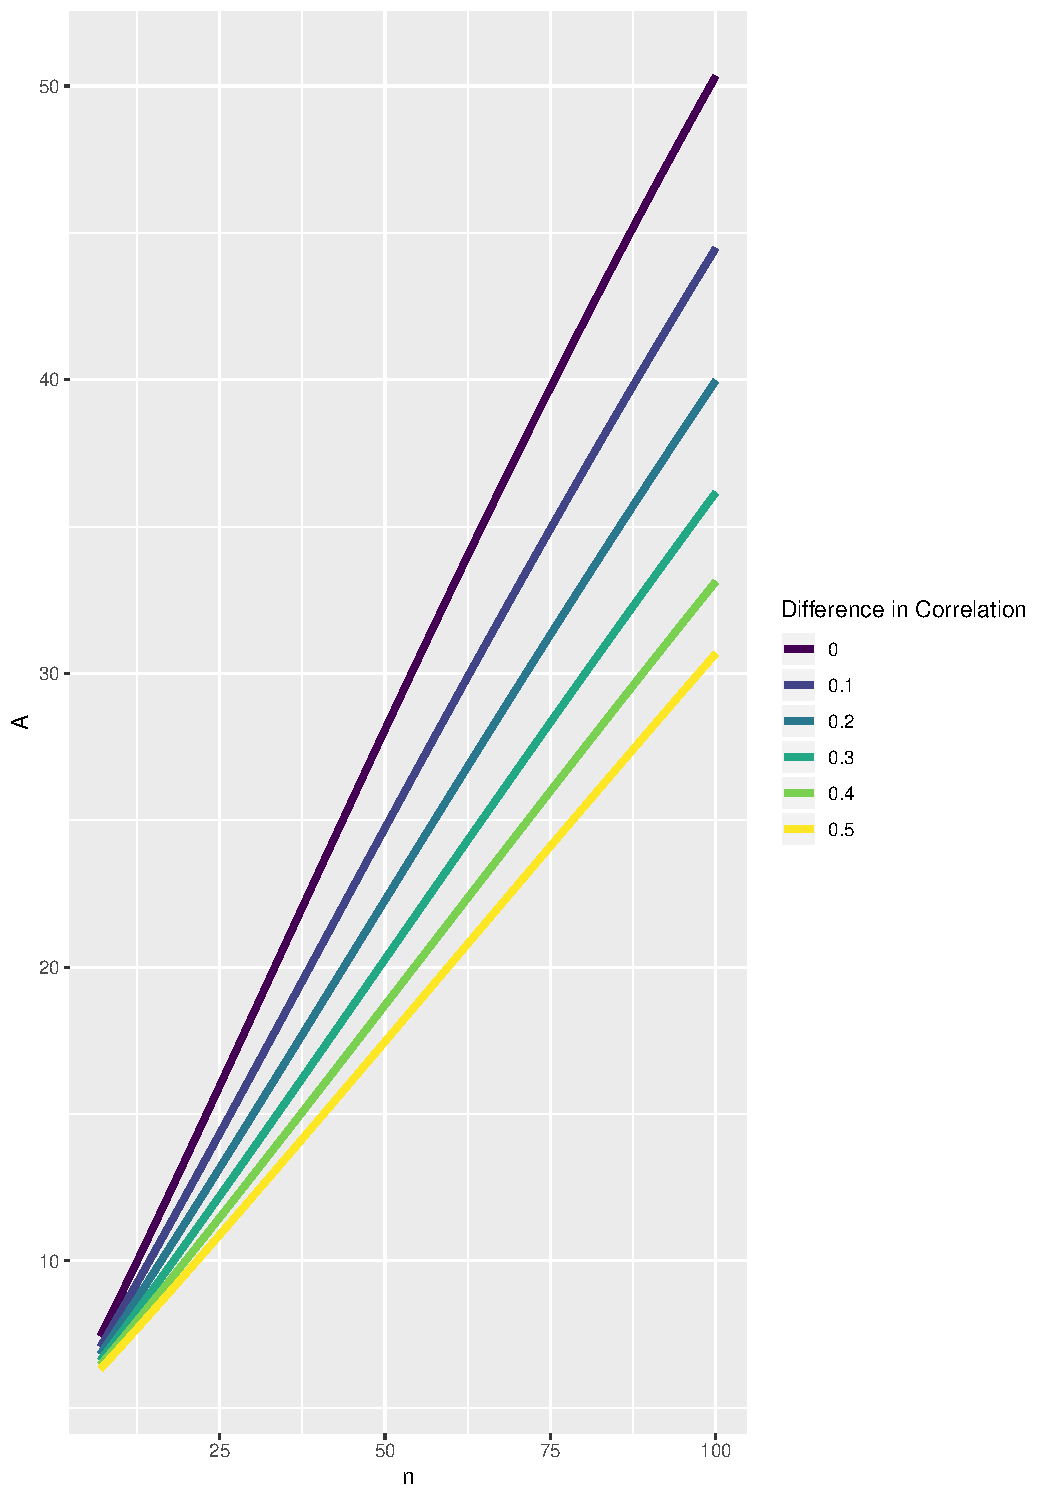
\includegraphics{SuperpowerValidation_files/figure-latex/unnamed-chunk-154-1.pdf}

We can reproduce this simulation:

\begin{Shaded}
\begin{Highlighting}[]
\CommentTok{# true effects (in this case, a double dissociation)}
\NormalTok{mu =}\StringTok{ }\KeywordTok{c}\NormalTok{(}\DecValTok{700}\NormalTok{, }\DecValTok{670}\NormalTok{, }\DecValTok{690}\NormalTok{, }\DecValTok{750}\NormalTok{) }
\NormalTok{sigma =}\StringTok{ }\DecValTok{150}  \CommentTok{# population standard deviation}
\NormalTok{n <-}\StringTok{ }\DecValTok{25}
\NormalTok{sd <-}\StringTok{ }\DecValTok{150}
\NormalTok{r <-}\StringTok{ }\FloatTok{0.4}
\NormalTok{string =}\StringTok{ "2w*2w"}
\NormalTok{alpha_level <-}\StringTok{ }\FloatTok{0.05}
\NormalTok{labelnames =}\StringTok{ }\KeywordTok{c}\NormalTok{(}\StringTok{"AGE"}\NormalTok{, }\StringTok{"old"}\NormalTok{, }\StringTok{"young"}\NormalTok{, }
               \StringTok{"COLOR"}\NormalTok{, }\StringTok{"blue"}\NormalTok{, }\StringTok{"red"}\NormalTok{)}

\NormalTok{design_result <-}\StringTok{ }\KeywordTok{ANOVA_design}\NormalTok{(}\DataTypeTok{design =}\NormalTok{ string,}
                              \DataTypeTok{n =}\NormalTok{ n, }
                              \DataTypeTok{mu =}\NormalTok{ mu, }
                              \DataTypeTok{sd =}\NormalTok{ sd, }
                              \DataTypeTok{r =}\NormalTok{ r, }
                              \DataTypeTok{labelnames =}\NormalTok{ labelnames)}
\end{Highlighting}
\end{Shaded}

\begin{Shaded}
\begin{Highlighting}[]
\NormalTok{simulation_result <-}\StringTok{ }\KeywordTok{ANOVA_power}\NormalTok{(design_result, }
                                 \DataTypeTok{alpha_level =} \FloatTok{0.05}\NormalTok{, }
                                 \DataTypeTok{nsims =}\NormalTok{ nsims)}
\end{Highlighting}
\end{Shaded}

\begin{table}[!h]

\caption{\label{tab:unnamed-chunk-157}Simulated ANOVA Result}
\centering
\begin{tabular}{l|r|r}
\hline
  & power & effect\_size\\
\hline
anova\_AGE & 30.60 & 0.1143202\\
\hline
anova\_COLOR & 9.41 & 0.0541130\\
\hline
anova\_AGE:COLOR & 46.22 & 0.1595391\\
\hline
\end{tabular}
\end{table}

\begin{Shaded}
\begin{Highlighting}[]
\NormalTok{exact_result <-}\StringTok{ }\KeywordTok{ANOVA_exact}\NormalTok{(design_result, }\DataTypeTok{alpha_level =}\NormalTok{ alpha_level)}
\end{Highlighting}
\end{Shaded}

\begin{verbatim}
## Power and Effect sizes for ANOVA tests
##             power partial_eta_squared cohen_f non_centrality
## AGE       30.4009              0.0864  0.3074         2.2685
## COLOR      9.5071              0.0171  0.1318         0.4167
## AGE:COLOR 45.9803              0.1351  0.3953         3.7500
## 
## Power and Effect sizes for contrasts
##                                            power effect_size
## p_AGE_old_COLOR_blue_AGE_old_COLOR_red     14.16     -0.1826
## p_AGE_old_COLOR_blue_AGE_young_COLOR_blue   5.98     -0.0609
## p_AGE_old_COLOR_blue_AGE_young_COLOR_red   30.91      0.3043
## p_AGE_old_COLOR_red_AGE_young_COLOR_blue    9.00      0.1217
## p_AGE_old_COLOR_red_AGE_young_COLOR_red    64.66      0.4869
## p_AGE_young_COLOR_blue_AGE_young_COLOR_red 41.80      0.3651
\end{verbatim}

\begin{table}[!h]

\caption{\label{tab:unnamed-chunk-159}Exact ANOVA Result}
\centering
\begin{tabular}{l|r|r|r|r}
\hline
  & power & partial\_eta\_squared & cohen\_f & non\_centrality\\
\hline
AGE & 30.400885 & 0.0863588 & 0.3074437 & 2.2685185\\
\hline
COLOR & 9.507147 & 0.0170648 & 0.1317616 & 0.4166667\\
\hline
AGE:COLOR & 45.980305 & 0.1351351 & 0.3952847 & 3.7500000\\
\hline
\end{tabular}
\end{table}

\hypertarget{part-5}{%
\section{Part 5}\label{part-5}}

\textbf{Credit for the non-centrality parameter for the interaction goes to Andrew Vigotsky}

\hypertarget{x2-anova-within-design}{%
\subsection{2x2 ANOVA, within design}\label{x2-anova-within-design}}

\citet{potvin2000statistical} simulate a wide range of repeated measure designs. They give an example of a 3x3 design, with the following correlation matrix:

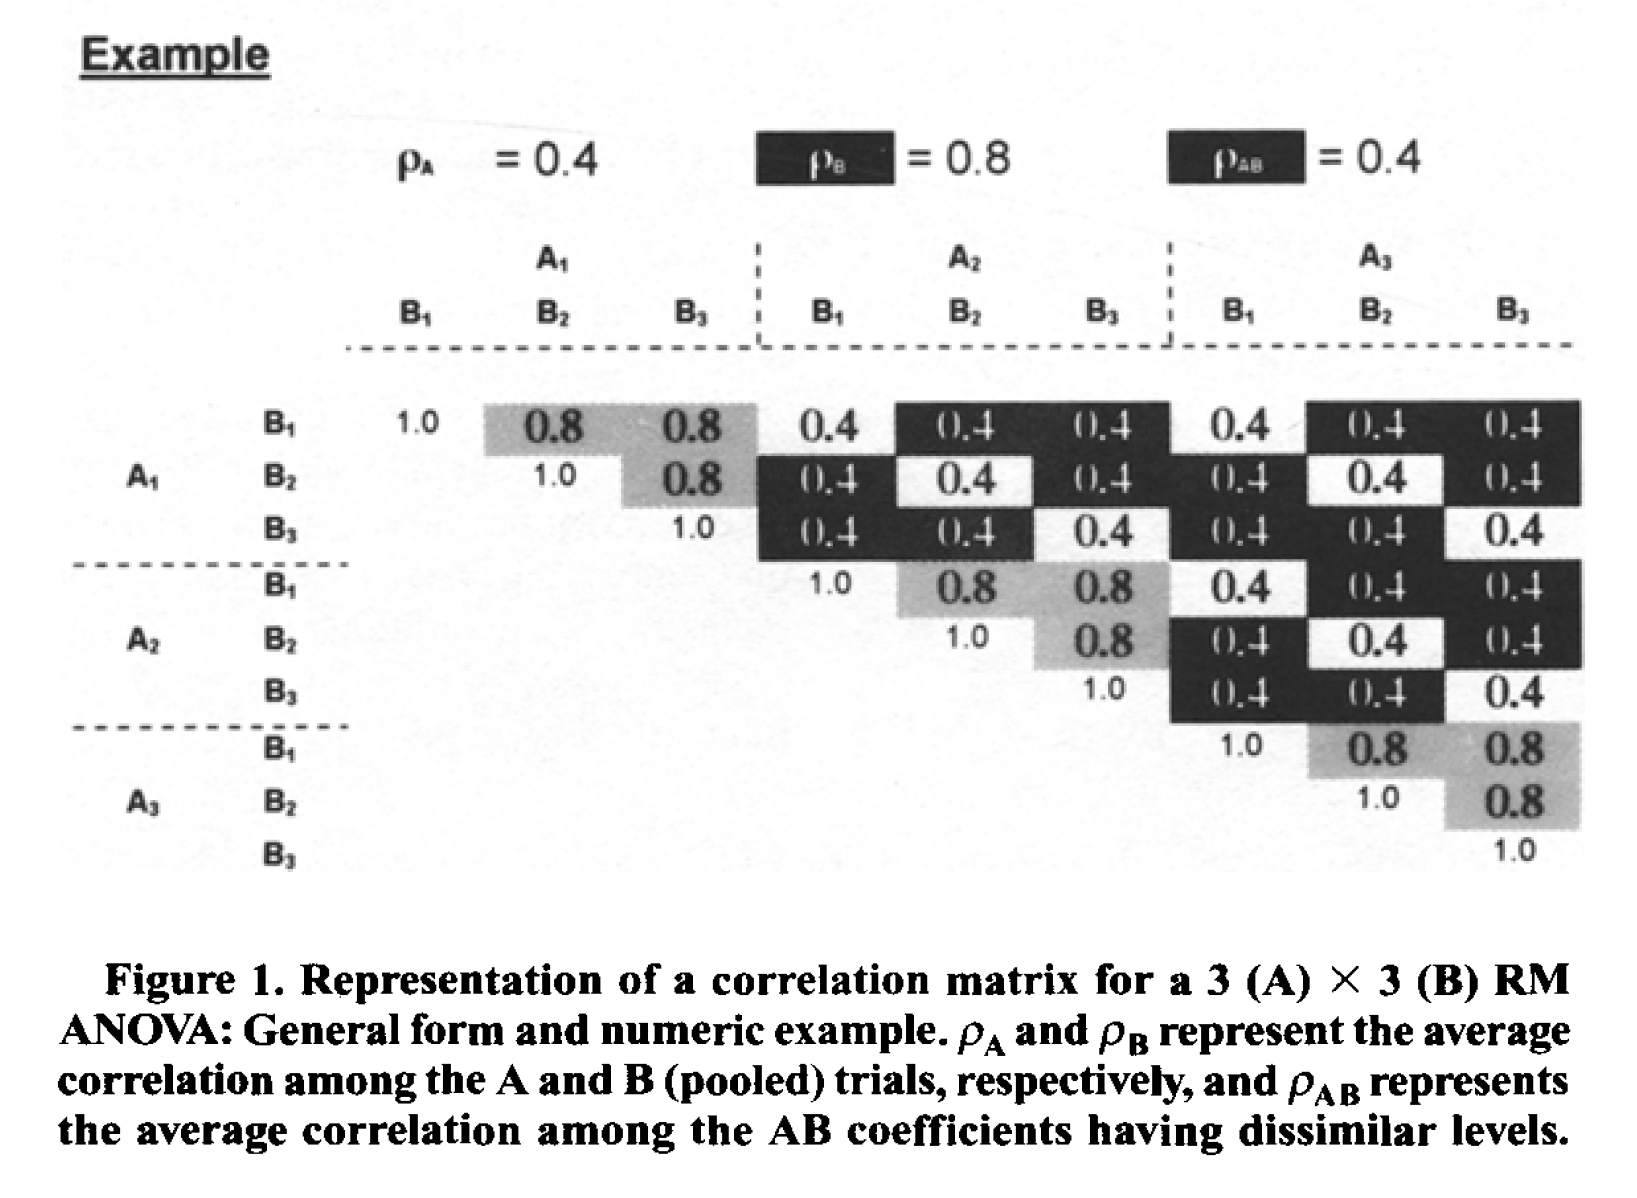
\includegraphics{screenshots/PS2000.png}

Variances were set to 1 (so all covariance matrices in their simulations were identical). In this specific example, the white fields are related to the correlation for the A main effect (these cells have the same level for B, but different levels of A). The grey cells are related to the main effect of B (the cells have the same level of A, but different levels of B). Finally, the black cells are related to the AxB interaction (they have different levels of A and B). The diagonal (all 1) relate to cells with the same levels of A and B.

\citet{potvin2000statistical} examine power for 2x2 within ANOVA designs and develop approximations of the error variance. For a design with 2 within factors (A and B) these are:

For the main effect of A:
\(\sigma _ { e } ^ { 2 } = \sigma ^ { 2 } ( 1 - \overline { \rho } _ { A } ) + \sigma ^ { 2 } ( q - 1 ) ( \overline { \rho } _ { B } - \overline { \rho } _ { AB } )\)

For the main effectof B:
\(\sigma _ { e } ^ { 2 } = \sigma ^ { 2 } ( 1 - \overline { \rho } _ { B } ) + \sigma ^ { 2 } ( p - 1 ) ( \overline { \rho } _ { A } - \overline { \rho } _ { A B } )\)

For the interaction between A and B:
\(\sigma _ { e } ^ { 2 } = \sigma ^ { 2 } ( 1 - \rho _ { \max } ) - \sigma ^ { 2 } ( \overline { \rho } _ { \min } - \overline { \rho } _ { AB } )\)

Let's now compare the formulas in \citet{potvin2000statistical} with \texttt{Superpower} with a simple scenario.

\begin{Shaded}
\begin{Highlighting}[]
\NormalTok{mu =}\StringTok{ }\KeywordTok{c}\NormalTok{(}\DecValTok{2}\NormalTok{,}\DecValTok{1}\NormalTok{,}\DecValTok{4}\NormalTok{,}\DecValTok{2}\NormalTok{) }
\NormalTok{n <-}\StringTok{ }\DecValTok{20}
\NormalTok{sd <-}\StringTok{ }\DecValTok{5}
\NormalTok{r <-}\StringTok{ }\FloatTok{.77}
\NormalTok{string =}\StringTok{ "2w*2w"}
\NormalTok{alpha_level <-}\StringTok{ }\FloatTok{0.05}


\NormalTok{design_result <-}\StringTok{ }\KeywordTok{ANOVA_design}\NormalTok{(}\DataTypeTok{design =}\NormalTok{ string,}
                              \DataTypeTok{n =}\NormalTok{ n, }
                              \DataTypeTok{mu =}\NormalTok{ mu, }
                              \DataTypeTok{sd =}\NormalTok{ sd, }
                              \DataTypeTok{r =}\NormalTok{ r, }
                              \DataTypeTok{labelnames =}\NormalTok{ labelnames,}
                              \DataTypeTok{plot =} \OtherTok{TRUE}\NormalTok{)}
\end{Highlighting}
\end{Shaded}

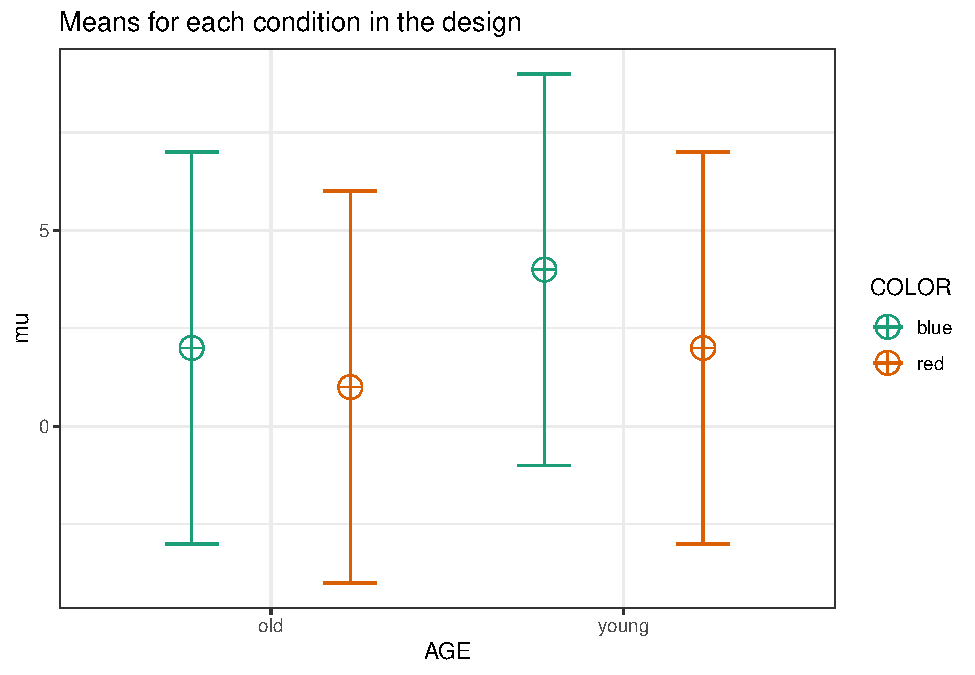
\includegraphics{SuperpowerValidation_files/figure-latex/unnamed-chunk-160-1.pdf}

\begin{Shaded}
\begin{Highlighting}[]
\NormalTok{design_result}\OperatorTok{$}\NormalTok{cor_mat}
\end{Highlighting}
\end{Shaded}

\begin{verbatim}
##            old_blue old_red young_blue young_red
## old_blue       1.00    0.77       0.77      0.77
## old_red        0.77    1.00       0.77      0.77
## young_blue     0.77    0.77       1.00      0.77
## young_red      0.77    0.77       0.77      1.00
\end{verbatim}

\begin{Shaded}
\begin{Highlighting}[]
\NormalTok{exact_result <-}\StringTok{ }\KeywordTok{ANOVA_exact}\NormalTok{(design_result,}
                            \DataTypeTok{alpha_level =}\NormalTok{ alpha_level,}
                            \DataTypeTok{verbose =} \OtherTok{FALSE}\NormalTok{)}
\end{Highlighting}
\end{Shaded}

\begin{table}[!h]

\caption{\label{tab:unnamed-chunk-162}Exact ANOVA Result}
\centering
\begin{tabular}{l|r|r|r|r}
\hline
  & power & partial\_eta\_squared & cohen\_f & non\_centrality\\
\hline
AGE & 75.61412 & 0.2917342 & 0.6417938 & 7.8260870\\
\hline
COLOR & 75.61412 & 0.2917342 & 0.6417938 & 7.8260870\\
\hline
AGE:COLOR & 14.36376 & 0.0437637 & 0.2139313 & 0.8695652\\
\hline
\end{tabular}
\end{table}

Further, as we use the analytical solution below, the variance components should be equal to the corresponding MSE from the \texttt{ANOVA\_exact} produced \texttt{anova\_table} object.

\begin{Shaded}
\begin{Highlighting}[]
\NormalTok{exact_result}\OperatorTok{$}\NormalTok{aov_result}\OperatorTok{$}\NormalTok{anova_table}
\end{Highlighting}
\end{Shaded}

\begin{verbatim}
## Anova Table (Type 3 tests)
## 
## Response: y
##           num Df den Df  MSE      F      pes  Pr(>F)  
## AGE            1     19 5.75 7.8261 0.291734 0.01149 *
## COLOR          1     19 5.75 7.8261 0.291734 0.01149 *
## AGE:COLOR      1     19 5.75 0.8696 0.043764 0.36278  
## ---
## Signif. codes:  0 '***' 0.001 '**' 0.01 '*' 0.05 '.' 0.1 ' ' 1
\end{verbatim}

We can try to use the formula in \citet{potvin2000statistical}.

\begin{Shaded}
\begin{Highlighting}[]
\NormalTok{k <-}\StringTok{ }\DecValTok{1} \CommentTok{#one group (because all factors are within)}

\NormalTok{rho_A <-}\StringTok{ }\FloatTok{.77} \CommentTok{#mean r for factor A}

\NormalTok{rho_B <-}\StringTok{ }\FloatTok{.77} \CommentTok{#mean r for factor B}

\NormalTok{rho_AB <-}\StringTok{ }\FloatTok{.77} \CommentTok{#mean r for factor AB}

\NormalTok{alpha <-}\StringTok{ }\FloatTok{0.05}

\NormalTok{sigma <-}\StringTok{ }\NormalTok{sd}

\NormalTok{m_A <-}\StringTok{ }\DecValTok{2} \CommentTok{#levels factor A}

\NormalTok{variance_e_A <-}\StringTok{ }\NormalTok{(sigma}\OperatorTok{^}\DecValTok{2} \OperatorTok{*}\StringTok{ }\NormalTok{(}\DecValTok{1} \OperatorTok{-}\StringTok{ }\NormalTok{rho_A) }\OperatorTok{+}\StringTok{ }
\StringTok{  }\NormalTok{sigma}\OperatorTok{^}\DecValTok{2} \OperatorTok{*}\StringTok{ }\NormalTok{(m_A }\OperatorTok{-}\StringTok{ }\DecValTok{1}\NormalTok{) }\OperatorTok{*}\StringTok{ }\NormalTok{(rho_B }\OperatorTok{-}\StringTok{ }\NormalTok{rho_AB) )}
\CommentTok{#Variance A}
\NormalTok{variance_e_A}
\end{Highlighting}
\end{Shaded}

\begin{verbatim}
## [1] 5.75
\end{verbatim}

\begin{Shaded}
\begin{Highlighting}[]
\NormalTok{m_B <-}\StringTok{ }\DecValTok{2} \CommentTok{#levels factor B}

\NormalTok{variance_e_B <-}\StringTok{ }\NormalTok{sigma}\OperatorTok{^}\DecValTok{2} \OperatorTok{*}\StringTok{ }\NormalTok{(}\DecValTok{1} \OperatorTok{-}\StringTok{ }\NormalTok{rho_B) }\OperatorTok{+}\StringTok{ }
\StringTok{  }\NormalTok{sigma}\OperatorTok{^}\DecValTok{2} \OperatorTok{*}\StringTok{ }\NormalTok{(m_B }\OperatorTok{-}\StringTok{ }\DecValTok{1}\NormalTok{) }\OperatorTok{*}\StringTok{ }\NormalTok{(rho_A }\OperatorTok{-}\StringTok{ }\NormalTok{rho_AB)}
\CommentTok{#Variance B}
\NormalTok{variance_e_B}
\end{Highlighting}
\end{Shaded}

\begin{verbatim}
## [1] 5.75
\end{verbatim}

\begin{Shaded}
\begin{Highlighting}[]
\NormalTok{variance_e_AB <-}
\StringTok{  }\NormalTok{(sigma }\OperatorTok{^}\StringTok{ }\DecValTok{2} \OperatorTok{*}\StringTok{ }\NormalTok{(}\DecValTok{1} \OperatorTok{-}\StringTok{ }\KeywordTok{max}\NormalTok{(rho_A, rho_B)) }\OperatorTok{-}\StringTok{ }
\StringTok{     }\NormalTok{sigma }\OperatorTok{^}\StringTok{ }\DecValTok{2} \OperatorTok{*}\StringTok{ }\NormalTok{(}\KeywordTok{min}\NormalTok{(rho_A,rho_B) }\OperatorTok{-}\StringTok{ }\NormalTok{rho_AB)) }
\CommentTok{#Variance AB}
\NormalTok{variance_e_AB}
\end{Highlighting}
\end{Shaded}

\begin{verbatim}
## [1] 5.75
\end{verbatim}

\begin{Shaded}
\begin{Highlighting}[]
\CommentTok{#Create a mean matrix}
\NormalTok{mean_mat <-}\StringTok{ }\KeywordTok{t}\NormalTok{(}\KeywordTok{matrix}\NormalTok{(mu, }\DataTypeTok{nrow =}\NormalTok{ m_B,}\DataTypeTok{ncol =}\NormalTok{ m_A)) }
\NormalTok{mean_mat}
\end{Highlighting}
\end{Shaded}

\begin{verbatim}
##      [,1] [,2]
## [1,]    2    1
## [2,]    4    2
\end{verbatim}

\begin{Shaded}
\begin{Highlighting}[]
\CommentTok{# Potvin & Schutz, 2000, formula 2, p. 348}
\CommentTok{# For main effect A}
\NormalTok{lambda_A <-}
\StringTok{  }\NormalTok{(n }\OperatorTok{*}\StringTok{ }\NormalTok{m_A }\OperatorTok{*}\StringTok{ }\KeywordTok{sum}\NormalTok{((}\KeywordTok{rowMeans}\NormalTok{(mean_mat) }\OperatorTok{-}\StringTok{ }
\StringTok{                   }\KeywordTok{mean}\NormalTok{(}\KeywordTok{rowMeans}\NormalTok{(mean_mat))) }\OperatorTok{^}\StringTok{ }\DecValTok{2}\NormalTok{) ) }\OperatorTok{/}\StringTok{ }\NormalTok{variance_e_A}
\NormalTok{  lambda_A}
\end{Highlighting}
\end{Shaded}

\begin{verbatim}
## [1] 7.826087
\end{verbatim}

\begin{Shaded}
\begin{Highlighting}[]
\CommentTok{#calculate degrees of freedom 1 - ignoring the sphericity correction}
\NormalTok{df1 <-}\StringTok{ }\NormalTok{(m_A }\OperatorTok{-}\StringTok{ }\DecValTok{1}\NormalTok{) }

\NormalTok{df2 <-}\StringTok{ }\NormalTok{(n }\OperatorTok{-}\StringTok{ }\NormalTok{k) }\OperatorTok{*}\StringTok{ }\NormalTok{(m_A }\OperatorTok{-}\StringTok{ }\DecValTok{1}\NormalTok{) }\CommentTok{#calculate degrees of freedom 2}

\NormalTok{F_critical <-}\StringTok{ }\KeywordTok{qf}\NormalTok{(alpha, }\CommentTok{# critical F-vaue}
\NormalTok{                 df1,}
\NormalTok{                 df2, }
                 \DataTypeTok{lower.tail =} \OtherTok{FALSE}\NormalTok{) }

\NormalTok{pow_A <-}\StringTok{ }\KeywordTok{pf}\NormalTok{(}\KeywordTok{qf}\NormalTok{(alpha, }\CommentTok{#power }
\NormalTok{             df1, }
\NormalTok{             df2, }
             \DataTypeTok{lower.tail =} \OtherTok{FALSE}\NormalTok{), }
\NormalTok{          df1, }
\NormalTok{          df2, }
\NormalTok{          lambda_A, }
          \DataTypeTok{lower.tail =} \OtherTok{FALSE}\NormalTok{)}
\NormalTok{pow_A}\OperatorTok{*}\DecValTok{100}
\end{Highlighting}
\end{Shaded}

\begin{verbatim}
## [1] 75.61412
\end{verbatim}

\begin{Shaded}
\begin{Highlighting}[]
\NormalTok{lambda_B <-}
\StringTok{  }\NormalTok{n }\OperatorTok{*}\StringTok{ }\NormalTok{m_B }\OperatorTok{*}\StringTok{ }\KeywordTok{sum}\NormalTok{((}\KeywordTok{colMeans}\NormalTok{(mean_mat) }\OperatorTok{-}\StringTok{ }
\StringTok{                   }\KeywordTok{mean}\NormalTok{(}\KeywordTok{colMeans}\NormalTok{(mean_mat))) }\OperatorTok{^}\StringTok{ }\DecValTok{2}\NormalTok{) }\OperatorTok{/}\StringTok{ }\NormalTok{variance_e_B }
\NormalTok{lambda_B}
\end{Highlighting}
\end{Shaded}

\begin{verbatim}
## [1] 7.826087
\end{verbatim}

\begin{Shaded}
\begin{Highlighting}[]
\NormalTok{df1 <-}\StringTok{ }\NormalTok{(m_B }\OperatorTok{-}\StringTok{ }\DecValTok{1}\NormalTok{) }\CommentTok{#calculate degrees of freedom 1}

\NormalTok{df2 <-}\StringTok{ }\NormalTok{(n }\OperatorTok{-}\StringTok{ }\NormalTok{k) }\OperatorTok{*}\StringTok{ }\NormalTok{(m_B }\OperatorTok{-}\StringTok{ }\DecValTok{1}\NormalTok{) }\CommentTok{#calculate degrees of freedom 2}

\NormalTok{F_critical <-}\StringTok{ }\KeywordTok{qf}\NormalTok{(alpha, }\CommentTok{# critical F-vaue}
\NormalTok{                 df1,}
\NormalTok{                 df2,}
                 \DataTypeTok{lower.tail =} \OtherTok{FALSE}\NormalTok{) }

\NormalTok{pow_B <-}\StringTok{ }\KeywordTok{pf}\NormalTok{(}\KeywordTok{qf}\NormalTok{(alpha, }\CommentTok{#power }
\NormalTok{             df1, }
\NormalTok{             df2, }
             \DataTypeTok{lower.tail =} \OtherTok{FALSE}\NormalTok{), }
\NormalTok{          df1, }
\NormalTok{          df2, }
\NormalTok{          lambda_B, }
          \DataTypeTok{lower.tail =} \OtherTok{FALSE}\NormalTok{)}


\NormalTok{pow_B}\OperatorTok{*}\DecValTok{100}
\end{Highlighting}
\end{Shaded}

\begin{verbatim}
## [1] 75.61412
\end{verbatim}

\begin{Shaded}
\begin{Highlighting}[]
\CommentTok{#Peform double summation courtesy of Andrew Vigotsky}
\NormalTok{term <-}\StringTok{ }\DecValTok{0}
\ControlFlowTok{for}\NormalTok{ (i }\ControlFlowTok{in} \DecValTok{1}\OperatorTok{:}\KeywordTok{nrow}\NormalTok{(mean_mat)) \{}
  \ControlFlowTok{for}\NormalTok{ (j }\ControlFlowTok{in} \DecValTok{1}\OperatorTok{:}\KeywordTok{ncol}\NormalTok{(mean_mat)) \{}
\NormalTok{    term <-}\StringTok{ }\NormalTok{(term }\OperatorTok{+}\StringTok{ }\NormalTok{(mean_mat[i,j] }\OperatorTok{-}\StringTok{ }
\StringTok{                       }\KeywordTok{mean}\NormalTok{(mean_mat[i,]) }\OperatorTok{-}\StringTok{ }
\StringTok{                       }\KeywordTok{mean}\NormalTok{(mean_mat[,j]) }\OperatorTok{+}\StringTok{ }\KeywordTok{mean}\NormalTok{(mean_mat))}\OperatorTok{^}\DecValTok{2}\NormalTok{)}
\NormalTok{  \}}
\NormalTok{\}}
\NormalTok{term}
\end{Highlighting}
\end{Shaded}

\begin{verbatim}
## [1] 0.25
\end{verbatim}

\begin{Shaded}
\begin{Highlighting}[]
\CommentTok{#Calculate lambda for interaction term}
\NormalTok{lambda_AB <-}\StringTok{ }\NormalTok{n}\OperatorTok{*}\NormalTok{term}\OperatorTok{/}\NormalTok{variance_e_AB}
\NormalTok{lambda_AB}
\end{Highlighting}
\end{Shaded}

\begin{verbatim}
## [1] 0.8695652
\end{verbatim}

\begin{Shaded}
\begin{Highlighting}[]
\NormalTok{df1 <-}\StringTok{ }\NormalTok{(m_A }\OperatorTok{-}\StringTok{ }\DecValTok{1}\NormalTok{) }\OperatorTok{*}\StringTok{ }\NormalTok{(m_B }\OperatorTok{-}\StringTok{ }\DecValTok{1}\NormalTok{)  }\CommentTok{#calculate degrees of freedom 1}
\NormalTok{df2 <-}
\NormalTok{(n }\OperatorTok{-}\StringTok{ }\NormalTok{k) }\OperatorTok{*}\StringTok{ }\NormalTok{(m_A }\OperatorTok{-}\StringTok{ }\DecValTok{1}\NormalTok{) }\OperatorTok{*}\StringTok{ }\NormalTok{(m_B }\OperatorTok{-}\StringTok{ }\DecValTok{1}\NormalTok{) }\CommentTok{#calculate degrees of freedom 2}
\NormalTok{F_critical <-}\StringTok{ }\KeywordTok{qf}\NormalTok{(alpha, }\CommentTok{# critical F-vaue}
\NormalTok{df1,}
\NormalTok{df2,}
\DataTypeTok{lower.tail =} \OtherTok{FALSE}\NormalTok{)}

\NormalTok{pow_AB <-}\StringTok{ }\KeywordTok{pf}\NormalTok{(}\KeywordTok{qf}\NormalTok{(alpha, }\CommentTok{#power}
\NormalTok{df1,}
\NormalTok{df2,}
\DataTypeTok{lower.tail =} \OtherTok{FALSE}\NormalTok{),}
\NormalTok{df1,}
\NormalTok{df2,}
\NormalTok{lambda_AB,}
\DataTypeTok{lower.tail =} \OtherTok{FALSE}\NormalTok{)}

\NormalTok{pow_AB}\OperatorTok{*}\DecValTok{100}
\end{Highlighting}
\end{Shaded}

\begin{verbatim}
## [1] 14.36376
\end{verbatim}

We can now compile all the analytical results into a single table, and see that the results match those from \texttt{ANOVA\_exact}.

\begin{table}[!h]

\caption{\label{tab:unnamed-chunk-166}Analytical Result}
\centering
\begin{tabular}{r|r|r}
\hline
variance & lambda & power\\
\hline
5.75 & 7.8260870 & 75.61412\\
\hline
5.75 & 7.8260870 & 75.61412\\
\hline
5.75 & 0.8695652 & 14.36376\\
\hline
\end{tabular}
\end{table}

And we can see in the simple scenario matches \texttt{ANOVA\_exact} and \texttt{ANOVA\_power} output.

Let's now extend to one of the simlations presented by \citet{potvin2000statistical} with a 3x3 solution.

\begin{Shaded}
\begin{Highlighting}[]
\NormalTok{mu =}\StringTok{ }\KeywordTok{c}\NormalTok{(}\DecValTok{2}\NormalTok{,}\DecValTok{1}\NormalTok{,}\DecValTok{4}\NormalTok{,}
       \DecValTok{2}\NormalTok{,.}\DecValTok{5}\NormalTok{,}\DecValTok{3}\NormalTok{,}
       \DecValTok{2}\NormalTok{,}\DecValTok{0}\NormalTok{,}\DecValTok{6}\NormalTok{) }
\NormalTok{n <-}\StringTok{ }\DecValTok{20}
\NormalTok{sd <-}\StringTok{ }\DecValTok{5}
\NormalTok{r <-}\StringTok{ }\KeywordTok{c}\NormalTok{(}\FloatTok{1.0}\NormalTok{,}\FloatTok{0.8}\NormalTok{,}\FloatTok{0.8}\NormalTok{,}\FloatTok{0.4}\NormalTok{,}\FloatTok{0.4}\NormalTok{,}\FloatTok{0.4}\NormalTok{,}\FloatTok{0.4}\NormalTok{,}\FloatTok{0.4}\NormalTok{,}\FloatTok{0.4}\NormalTok{,}
       \FloatTok{0.8}\NormalTok{,}\FloatTok{1.0}\NormalTok{,}\FloatTok{0.8}\NormalTok{,}\FloatTok{0.4}\NormalTok{,}\FloatTok{0.4}\NormalTok{,}\FloatTok{0.4}\NormalTok{,}\FloatTok{0.4}\NormalTok{,}\FloatTok{0.4}\NormalTok{,}\FloatTok{0.4}\NormalTok{,}
       \FloatTok{0.8}\NormalTok{,}\FloatTok{0.8}\NormalTok{,}\FloatTok{1.0}\NormalTok{,}\FloatTok{0.4}\NormalTok{,}\FloatTok{0.4}\NormalTok{,}\FloatTok{0.4}\NormalTok{,}\FloatTok{0.4}\NormalTok{,}\FloatTok{0.4}\NormalTok{,}\FloatTok{0.4}\NormalTok{,}
       \FloatTok{0.4}\NormalTok{,}\FloatTok{0.4}\NormalTok{,}\FloatTok{0.4}\NormalTok{,}\FloatTok{1.0}\NormalTok{,}\FloatTok{0.8}\NormalTok{,}\FloatTok{0.8}\NormalTok{,}\FloatTok{0.4}\NormalTok{,}\FloatTok{0.4}\NormalTok{,}\FloatTok{0.4}\NormalTok{,}
       \FloatTok{0.4}\NormalTok{,}\FloatTok{0.4}\NormalTok{,}\FloatTok{0.4}\NormalTok{,}\FloatTok{0.8}\NormalTok{,}\FloatTok{1.0}\NormalTok{,}\FloatTok{0.8}\NormalTok{,}\FloatTok{0.4}\NormalTok{,}\FloatTok{0.4}\NormalTok{,}\FloatTok{0.4}\NormalTok{,}
       \FloatTok{0.4}\NormalTok{,}\FloatTok{0.4}\NormalTok{,}\FloatTok{0.4}\NormalTok{,}\FloatTok{0.8}\NormalTok{,}\FloatTok{0.8}\NormalTok{,}\FloatTok{1.0}\NormalTok{,}\FloatTok{0.4}\NormalTok{,}\FloatTok{0.4}\NormalTok{,}\FloatTok{0.4}\NormalTok{,}
       \FloatTok{0.4}\NormalTok{,}\FloatTok{0.4}\NormalTok{,}\FloatTok{0.4}\NormalTok{,}\FloatTok{0.4}\NormalTok{,}\FloatTok{0.4}\NormalTok{,}\FloatTok{0.4}\NormalTok{,}\FloatTok{1.0}\NormalTok{,}\FloatTok{0.8}\NormalTok{,}\FloatTok{0.8}\NormalTok{,}
       \FloatTok{0.4}\NormalTok{,}\FloatTok{0.4}\NormalTok{,}\FloatTok{0.4}\NormalTok{,}\FloatTok{0.4}\NormalTok{,}\FloatTok{0.4}\NormalTok{,}\FloatTok{0.4}\NormalTok{,}\FloatTok{0.8}\NormalTok{,}\FloatTok{1.0}\NormalTok{,}\FloatTok{0.8}\NormalTok{,}
       \FloatTok{0.4}\NormalTok{,}\FloatTok{0.4}\NormalTok{,}\FloatTok{0.4}\NormalTok{,}\FloatTok{0.4}\NormalTok{,}\FloatTok{0.4}\NormalTok{,}\FloatTok{0.4}\NormalTok{,}\FloatTok{0.8}\NormalTok{,}\FloatTok{0.8}\NormalTok{,}\FloatTok{1.0}\NormalTok{)}


\NormalTok{string =}\StringTok{ "3w*3w"}
\NormalTok{alpha_level <-}\StringTok{ }\FloatTok{0.05}

\NormalTok{design_result <-}\StringTok{ }\KeywordTok{ANOVA_design}\NormalTok{(}\DataTypeTok{design =}\NormalTok{ string,}
                              \DataTypeTok{n =}\NormalTok{ n, }
                              \DataTypeTok{mu =}\NormalTok{ mu, }
                              \DataTypeTok{sd =}\NormalTok{ sd, }
                              \DataTypeTok{r =}\NormalTok{ r, }
                              \DataTypeTok{plot =} \OtherTok{TRUE}\NormalTok{)}
\end{Highlighting}
\end{Shaded}

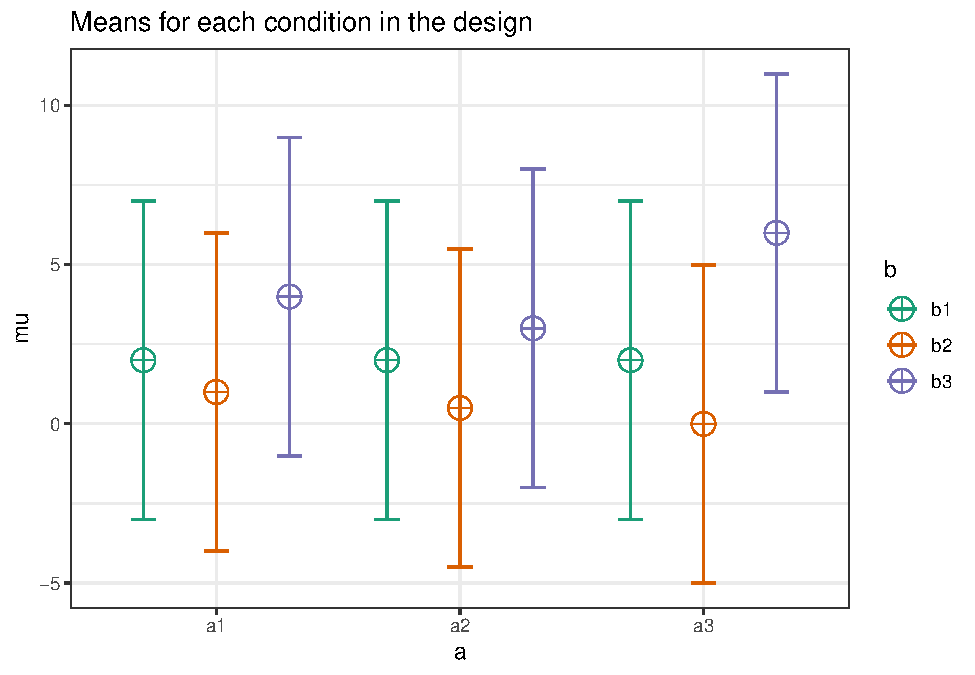
\includegraphics{SuperpowerValidation_files/figure-latex/unnamed-chunk-167-1.pdf}

\begin{Shaded}
\begin{Highlighting}[]
\NormalTok{design_result}\OperatorTok{$}\NormalTok{cor_mat}
\end{Highlighting}
\end{Shaded}

\begin{verbatim}
##       a1_b1 a1_b2 a1_b3 a2_b1 a2_b2 a2_b3 a3_b1 a3_b2 a3_b3
## a1_b1   1.0   0.8   0.8   0.4   0.4   0.4   0.4   0.4   0.4
## a1_b2   0.8   1.0   0.8   0.4   0.4   0.4   0.4   0.4   0.4
## a1_b3   0.8   0.8   1.0   0.4   0.4   0.4   0.4   0.4   0.4
## a2_b1   0.4   0.4   0.4   1.0   0.8   0.8   0.4   0.4   0.4
## a2_b2   0.4   0.4   0.4   0.8   1.0   0.8   0.4   0.4   0.4
## a2_b3   0.4   0.4   0.4   0.8   0.8   1.0   0.4   0.4   0.4
## a3_b1   0.4   0.4   0.4   0.4   0.4   0.4   1.0   0.8   0.8
## a3_b2   0.4   0.4   0.4   0.4   0.4   0.4   0.8   1.0   0.8
## a3_b3   0.4   0.4   0.4   0.4   0.4   0.4   0.8   0.8   1.0
\end{verbatim}

The design now matches the correlation matrix in Figure 1 of \citet{potvin2000statistical}.

And we can estimate power with \texttt{ANOVA\_exact}.

\begin{Shaded}
\begin{Highlighting}[]
\NormalTok{exact_result <-}\StringTok{ }\KeywordTok{ANOVA_exact}\NormalTok{(design_result,}
                            \DataTypeTok{alpha_level =}\NormalTok{ alpha_level,}
                            \DataTypeTok{verbose =} \OtherTok{FALSE}\NormalTok{)}
\end{Highlighting}
\end{Shaded}

\begin{table}[!h]

\caption{\label{tab:unnamed-chunk-169}Exact ANOVA Result}
\centering
\begin{tabular}{l|r|r|r|r}
\hline
  & power & partial\_eta\_squared & cohen\_f & non\_centrality\\
\hline
a & 9.441726 & 0.0156250 & 0.1259882 & 0.6031746\\
\hline
b & 100.000000 & 0.7020906 & 1.5351629 & 89.5555556\\
\hline
a:b & 90.092634 & 0.1778846 & 0.4651605 & 16.4444444\\
\hline
\end{tabular}
\end{table}

Further, as we use the analytical solution below, the variance components should be equal to the corresponding MSE from the \texttt{ANOVA\_exact} produced \texttt{anova\_table} object.

\begin{Shaded}
\begin{Highlighting}[]
\NormalTok{exact_result}\OperatorTok{$}\NormalTok{aov_result}\OperatorTok{$}\NormalTok{anova_table}
\end{Highlighting}
\end{Shaded}

\begin{verbatim}
## Anova Table (Type 3 tests)
## 
## Response: y
##     num Df den Df MSE       F     pes          Pr(>F)    
## a        2     38  35  0.3016 0.01563        0.741397    
## b        2     38   5 44.7778 0.70209 0.0000000001018 ***
## a:b      4     76   5  4.1111 0.17788        0.004542 ** 
## ---
## Signif. codes:  0 '***' 0.001 '**' 0.01 '*' 0.05 '.' 0.1 ' ' 1
\end{verbatim}

\begin{Shaded}
\begin{Highlighting}[]
\NormalTok{k <-}\StringTok{ }\DecValTok{1} \CommentTok{#one group (because all factors are within)}

\NormalTok{rho_A <-}\StringTok{ }\FloatTok{.4} \CommentTok{#mean r for factor A}

\NormalTok{rho_B <-}\StringTok{ }\FloatTok{.8} \CommentTok{#mean r for factor B}

\NormalTok{rho_AB <-}\StringTok{ }\FloatTok{.4} \CommentTok{#mean r for factor AB}

\NormalTok{alpha <-}\StringTok{ }\FloatTok{0.05}

\NormalTok{sigma <-}\StringTok{ }\NormalTok{sd}

\NormalTok{m_A <-}\StringTok{ }\DecValTok{3} \CommentTok{#levels factor A}

\NormalTok{variance_e_A <-}\StringTok{ }\NormalTok{sigma}\OperatorTok{^}\DecValTok{2} \OperatorTok{*}\StringTok{ }\NormalTok{(}\DecValTok{1} \OperatorTok{-}\StringTok{ }\NormalTok{rho_A) }\OperatorTok{+}\StringTok{ }
\StringTok{  }\NormalTok{sigma}\OperatorTok{^}\DecValTok{2} \OperatorTok{*}\StringTok{ }\NormalTok{(m_A }\OperatorTok{-}\StringTok{ }\DecValTok{1}\NormalTok{) }\OperatorTok{*}\StringTok{ }\NormalTok{(rho_B }\OperatorTok{-}\StringTok{ }\NormalTok{rho_AB) }
\CommentTok{#Variance A}
\NormalTok{variance_e_A}
\end{Highlighting}
\end{Shaded}

\begin{verbatim}
## [1] 35
\end{verbatim}

\begin{Shaded}
\begin{Highlighting}[]
\NormalTok{m_B <-}\StringTok{ }\DecValTok{3} \CommentTok{#levels factor B}

\NormalTok{variance_e_B <-}\StringTok{ }\NormalTok{sigma}\OperatorTok{^}\DecValTok{2} \OperatorTok{*}\StringTok{ }\NormalTok{(}\DecValTok{1} \OperatorTok{-}\StringTok{ }\NormalTok{rho_B) }\OperatorTok{+}\StringTok{ }
\StringTok{  }\NormalTok{sigma}\OperatorTok{^}\DecValTok{2} \OperatorTok{*}\StringTok{ }\NormalTok{(m_B }\OperatorTok{-}\StringTok{ }\DecValTok{1}\NormalTok{) }\OperatorTok{*}\StringTok{ }\NormalTok{(rho_A }\OperatorTok{-}\StringTok{ }\NormalTok{rho_AB)}
\CommentTok{#Variance B}
\NormalTok{variance_e_B}
\end{Highlighting}
\end{Shaded}

\begin{verbatim}
## [1] 5
\end{verbatim}

\begin{Shaded}
\begin{Highlighting}[]
\NormalTok{variance_e_AB <-}
\StringTok{  }\NormalTok{(sigma }\OperatorTok{^}\StringTok{ }\DecValTok{2} \OperatorTok{*}\StringTok{ }\NormalTok{(}\DecValTok{1} \OperatorTok{-}\StringTok{ }\KeywordTok{max}\NormalTok{(rho_A, rho_B)) }\OperatorTok{-}\StringTok{ }
\StringTok{     }\NormalTok{sigma }\OperatorTok{^}\StringTok{ }\DecValTok{2} \OperatorTok{*}\StringTok{ }\NormalTok{(}\KeywordTok{min}\NormalTok{(rho_A,rho_B) }\OperatorTok{-}\StringTok{ }\NormalTok{rho_AB)) }
\CommentTok{#Variance AB}
\NormalTok{variance_e_AB}
\end{Highlighting}
\end{Shaded}

\begin{verbatim}
## [1] 5
\end{verbatim}

\begin{Shaded}
\begin{Highlighting}[]
\CommentTok{#Create a mean matrix}
\NormalTok{mean_mat <-}\StringTok{ }\KeywordTok{t}\NormalTok{(}\KeywordTok{matrix}\NormalTok{(mu, }\DataTypeTok{nrow =}\NormalTok{ m_B,}\DataTypeTok{ncol =}\NormalTok{ m_A)) }
\NormalTok{mean_mat}
\end{Highlighting}
\end{Shaded}

\begin{verbatim}
##      [,1] [,2] [,3]
## [1,]    2  1.0    4
## [2,]    2  0.5    3
## [3,]    2  0.0    6
\end{verbatim}

\begin{Shaded}
\begin{Highlighting}[]
\CommentTok{# Potvin & Schutz, 2000, formula 2, p. 348}
\CommentTok{# For main effect A}
\NormalTok{lambda_A <-}
\StringTok{  }\NormalTok{(n }\OperatorTok{*}\StringTok{ }\NormalTok{m_A }\OperatorTok{*}\StringTok{ }\KeywordTok{sum}\NormalTok{((}\KeywordTok{rowMeans}\NormalTok{(mean_mat) }\OperatorTok{-}\StringTok{ }
\StringTok{                   }\KeywordTok{mean}\NormalTok{(}\KeywordTok{rowMeans}\NormalTok{(mean_mat))) }\OperatorTok{^}\StringTok{ }\DecValTok{2}\NormalTok{) ) }\OperatorTok{/}\StringTok{ }\NormalTok{variance_e_A}
\NormalTok{  lambda_A}
\end{Highlighting}
\end{Shaded}

\begin{verbatim}
## [1] 0.6031746
\end{verbatim}

\begin{Shaded}
\begin{Highlighting}[]
\CommentTok{#calculate degrees of freedom 1 - ignoring the sphericity correction}
\NormalTok{df1 <-}\StringTok{ }\NormalTok{(m_A }\OperatorTok{-}\StringTok{ }\DecValTok{1}\NormalTok{) }

\NormalTok{df2 <-}\StringTok{ }\NormalTok{(n }\OperatorTok{-}\StringTok{ }\NormalTok{k) }\OperatorTok{*}\StringTok{ }\NormalTok{(m_A }\OperatorTok{-}\StringTok{ }\DecValTok{1}\NormalTok{) }\CommentTok{#calculate degrees of freedom 2}

\NormalTok{F_critical <-}\StringTok{ }\KeywordTok{qf}\NormalTok{(alpha, }\CommentTok{# critical F-vaue}
\NormalTok{                 df1,}
\NormalTok{                 df2, }
                 \DataTypeTok{lower.tail =} \OtherTok{FALSE}\NormalTok{) }

\NormalTok{pow_A <-}\StringTok{ }\KeywordTok{pf}\NormalTok{(}\KeywordTok{qf}\NormalTok{(alpha, }\CommentTok{#power }
\NormalTok{             df1, }
\NormalTok{             df2, }
             \DataTypeTok{lower.tail =} \OtherTok{FALSE}\NormalTok{), }
\NormalTok{          df1, }
\NormalTok{          df2, }
\NormalTok{          lambda_A, }
          \DataTypeTok{lower.tail =} \OtherTok{FALSE}\NormalTok{)}
\NormalTok{pow_A}\OperatorTok{*}\DecValTok{100}
\end{Highlighting}
\end{Shaded}

\begin{verbatim}
## [1] 9.441726
\end{verbatim}

\begin{Shaded}
\begin{Highlighting}[]
\NormalTok{lambda_B <-}
\StringTok{  }\NormalTok{n }\OperatorTok{*}\StringTok{ }\NormalTok{m_B }\OperatorTok{*}\StringTok{ }\KeywordTok{sum}\NormalTok{((}\KeywordTok{colMeans}\NormalTok{(mean_mat) }\OperatorTok{-}\StringTok{ }
\StringTok{                   }\KeywordTok{mean}\NormalTok{(}\KeywordTok{colMeans}\NormalTok{(mean_mat))) }\OperatorTok{^}\StringTok{ }\DecValTok{2}\NormalTok{) }\OperatorTok{/}\StringTok{ }\NormalTok{variance_e_B }
\NormalTok{lambda_B}
\end{Highlighting}
\end{Shaded}

\begin{verbatim}
## [1] 89.55556
\end{verbatim}

\begin{Shaded}
\begin{Highlighting}[]
\NormalTok{df1 <-}\StringTok{ }\NormalTok{(m_B }\OperatorTok{-}\StringTok{ }\DecValTok{1}\NormalTok{) }\CommentTok{#calculate degrees of freedom 1}

\NormalTok{df2 <-}\StringTok{ }\NormalTok{(n }\OperatorTok{-}\StringTok{ }\NormalTok{k) }\OperatorTok{*}\StringTok{ }\NormalTok{(m_B }\OperatorTok{-}\StringTok{ }\DecValTok{1}\NormalTok{) }\CommentTok{#calculate degrees of freedom 2}

\NormalTok{F_critical <-}\StringTok{ }\KeywordTok{qf}\NormalTok{(alpha, }\CommentTok{# critical F-vaue}
\NormalTok{                 df1,}
\NormalTok{                 df2,}
                 \DataTypeTok{lower.tail =} \OtherTok{FALSE}\NormalTok{) }

\NormalTok{pow_B <-}\StringTok{ }\KeywordTok{pf}\NormalTok{(}\KeywordTok{qf}\NormalTok{(alpha, }\CommentTok{#power }
\NormalTok{             df1, }
\NormalTok{             df2, }
             \DataTypeTok{lower.tail =} \OtherTok{FALSE}\NormalTok{), }
\NormalTok{          df1, }
\NormalTok{          df2, }
\NormalTok{          lambda_B, }
          \DataTypeTok{lower.tail =} \OtherTok{FALSE}\NormalTok{)}


\NormalTok{pow_B}\OperatorTok{*}\DecValTok{100}
\end{Highlighting}
\end{Shaded}

\begin{verbatim}
## [1] 100
\end{verbatim}

\begin{Shaded}
\begin{Highlighting}[]
\CommentTok{#Peform double summation courtesy of Andrew Vigotsky}
\NormalTok{term <-}\StringTok{ }\DecValTok{0}
\ControlFlowTok{for}\NormalTok{ (i }\ControlFlowTok{in} \DecValTok{1}\OperatorTok{:}\KeywordTok{nrow}\NormalTok{(mean_mat)) \{}
  \ControlFlowTok{for}\NormalTok{ (j }\ControlFlowTok{in} \DecValTok{1}\OperatorTok{:}\KeywordTok{ncol}\NormalTok{(mean_mat)) \{}
\NormalTok{    term <-}\StringTok{ }\NormalTok{((term }\OperatorTok{+}\StringTok{ }\NormalTok{(mean_mat[i,j] }\OperatorTok{-}
\StringTok{                        }\KeywordTok{mean}\NormalTok{(mean_mat[i,]) }\OperatorTok{-}\StringTok{ }
\StringTok{                        }\KeywordTok{mean}\NormalTok{(mean_mat[,j]) }\OperatorTok{+}\StringTok{ }\KeywordTok{mean}\NormalTok{(mean_mat))}\OperatorTok{^}\DecValTok{2}\NormalTok{))}
\NormalTok{  \}}
\NormalTok{\}}
\NormalTok{term}
\end{Highlighting}
\end{Shaded}

\begin{verbatim}
## [1] 4.111111
\end{verbatim}

\begin{Shaded}
\begin{Highlighting}[]
\CommentTok{#Calculate lambda for interaction term}
\NormalTok{lambda_AB <-}\StringTok{ }\NormalTok{n}\OperatorTok{*}\NormalTok{term}\OperatorTok{/}\NormalTok{variance_e_AB}
\NormalTok{lambda_AB}
\end{Highlighting}
\end{Shaded}

\begin{verbatim}
## [1] 16.44444
\end{verbatim}

\begin{Shaded}
\begin{Highlighting}[]
\NormalTok{df1 <-}\StringTok{ }\NormalTok{(m_A }\OperatorTok{-}\StringTok{ }\DecValTok{1}\NormalTok{) }\OperatorTok{*}\StringTok{ }\NormalTok{(m_B }\OperatorTok{-}\StringTok{ }\DecValTok{1}\NormalTok{)  }\CommentTok{#calculate degrees of freedom 1}
\NormalTok{df2 <-}
\NormalTok{(n }\OperatorTok{-}\StringTok{ }\NormalTok{k) }\OperatorTok{*}\StringTok{ }\NormalTok{(m_A }\OperatorTok{-}\StringTok{ }\DecValTok{1}\NormalTok{) }\OperatorTok{*}\StringTok{ }\NormalTok{(m_B }\OperatorTok{-}\StringTok{ }\DecValTok{1}\NormalTok{) }\CommentTok{#calculate degrees of freedom 2}
\NormalTok{F_critical <-}\StringTok{ }\KeywordTok{qf}\NormalTok{(alpha, }\CommentTok{# critical F-vaue}
\NormalTok{df1,}
\NormalTok{df2,}
\DataTypeTok{lower.tail =} \OtherTok{FALSE}\NormalTok{)}

\NormalTok{pow_AB <-}\StringTok{ }\KeywordTok{pf}\NormalTok{(}\KeywordTok{qf}\NormalTok{(alpha, }\CommentTok{#power}
\NormalTok{df1,}
\NormalTok{df2,}
\DataTypeTok{lower.tail =} \OtherTok{FALSE}\NormalTok{),}
\NormalTok{df1,}
\NormalTok{df2,}
\NormalTok{lambda_AB,}
\DataTypeTok{lower.tail =} \OtherTok{FALSE}\NormalTok{)}

\NormalTok{pow_AB}\OperatorTok{*}\DecValTok{100}
\end{Highlighting}
\end{Shaded}

\begin{verbatim}
## [1] 90.09263
\end{verbatim}

Again, when we compile all the analytical results into a single table we can see that the results match those from \texttt{ANOVA\_exact}.

\begin{table}[!h]

\caption{\label{tab:unnamed-chunk-173}Analytical Result}
\centering
\begin{tabular}{r|r|r}
\hline
variance & lambda & power\\
\hline
35 & 0.6031746 & 9.441726\\
\hline
5 & 89.5555556 & 100.000000\\
\hline
5 & 16.4444444 & 90.092634\\
\hline
\end{tabular}
\end{table}

\hypertarget{multivariate-anova-manova}{%
\section{Multivariate ANOVA (MANOVA)}\label{multivariate-anova-manova}}

A large proportion of research with within-subjects manipulations, or repeated measures, rely upon the ``univariate'' approach \citep{maxwell_designing_2004}. While this approach is valid, when corrections for sphercity are applied, it may not be the most powerful or informative analysis plan. Instead, researchers should consider a multivariate analysis (MANOVA). While the MANOVA is not ``assumption free'' it does not assume sphercity which makes it a very attractive analytical tool and the preferred method of analysis for some {[}\citet{maxwell_designing_2004}.

For a simple one-way repeated measures design, there are some simple guidelines for power analysis set forth by \citet{maxwell_designing_2004} (pg. 750). All that is needed in the effect size calculated as:
\[ d = \frac{\mu_{max}-\mu_{min}}{\sigma} \]
This assumes that each level has a common standard deviation (i.e., there is only 1 \texttt{sd} input for the design).

In addition, the non-centrality parameter of the \emph{F}-statistic can be estimated from \citet{vonesh1986sample} equations as the following:
\[ \delta^2 = \frac{n \cdot d^2}{2\cdot(1-\rho_{min} )} \]
\newpage
Let us assume we have a \texttt{2w} design with \texttt{mu\ =\ c(0,0.5)}, a common standard deviation of 1 (\texttt{sd=1}), and correlation between \texttt{a1} and \texttt{a2} of r = .4 and a total sample size of 15 (\texttt{n\ =\ 15}) participants.
Power could then be calculated with the following \texttt{R} code.

\begin{Shaded}
\begin{Highlighting}[]
\NormalTok{mu =}\StringTok{ }\KeywordTok{c}\NormalTok{(}\DecValTok{0}\NormalTok{,}\FloatTok{0.5}\NormalTok{)}
\NormalTok{rho =}\StringTok{ }\FloatTok{.4}
\NormalTok{sd =}\StringTok{ }\DecValTok{2}
\NormalTok{n =}\StringTok{ }\DecValTok{15}
\NormalTok{d =}\StringTok{ }\NormalTok{(}\KeywordTok{max}\NormalTok{(mu)}\OperatorTok{-}\KeywordTok{min}\NormalTok{(mu))}\OperatorTok{/}\NormalTok{sd}
\NormalTok{noncentrality =}\StringTok{ }\NormalTok{((n}\OperatorTok{*}\NormalTok{d}\OperatorTok{^}\DecValTok{2}\NormalTok{) }\OperatorTok{/}\StringTok{ }\NormalTok{(}\DecValTok{2}\OperatorTok{*}\NormalTok{(}\DecValTok{1}\OperatorTok{-}\KeywordTok{min}\NormalTok{(rho))))}
\NormalTok{noncentrality}
\end{Highlighting}
\end{Shaded}

\begin{verbatim}
## [1] 0.78125
\end{verbatim}

\begin{Shaded}
\begin{Highlighting}[]
\CommentTok{#Critical F}
\NormalTok{Ft <-}\StringTok{ }\KeywordTok{qf}\NormalTok{((}\DecValTok{1} \OperatorTok{-}\StringTok{ }\FloatTok{.05}\NormalTok{), }\DecValTok{1}\NormalTok{, }\DecValTok{14}\NormalTok{)}
\NormalTok{Ft}
\end{Highlighting}
\end{Shaded}

\begin{verbatim}
## [1] 4.60011
\end{verbatim}

\begin{Shaded}
\begin{Highlighting}[]
\CommentTok{#Power}
\NormalTok{power <-}\StringTok{ }\NormalTok{(}\DecValTok{1} \OperatorTok{-}\StringTok{ }\KeywordTok{pf}\NormalTok{(Ft,}
                 \DecValTok{1}\NormalTok{,}
                 \DecValTok{14}\NormalTok{,}
\NormalTok{                 noncentrality)) }\OperatorTok{*}\StringTok{ }\DecValTok{100}
\NormalTok{power}
\end{Highlighting}
\end{Shaded}

\begin{verbatim}
## [1] 13.07682
\end{verbatim}

\newpage

Now we replicate in \texttt{Superpower}.

\begin{Shaded}
\begin{Highlighting}[]
\NormalTok{design_result <-}\StringTok{ }\KeywordTok{ANOVA_design}\NormalTok{(}\StringTok{"2w"}\NormalTok{,}
                              \DataTypeTok{n =}\NormalTok{ n,}
                              \DataTypeTok{r =}\NormalTok{ rho,}
                              \DataTypeTok{sd =}\NormalTok{ sd,}
                              \DataTypeTok{mu =}\NormalTok{ mu)}

\NormalTok{exact_result <-}\StringTok{ }\KeywordTok{ANOVA_exact}\NormalTok{(design_result, }\DataTypeTok{verbose =} \OtherTok{FALSE}\NormalTok{)}
\end{Highlighting}
\end{Shaded}

\begin{table}[!h]

\caption{\label{tab:unnamed-chunk-177}MANOVA Result}
\centering
\begin{tabular}{l|r|r|r|r}
\hline
  & power & pillai\_trace & cohen\_f & non\_centrality\\
\hline
(Intercept) & 8.401182 & 0.0233572 & 0.1546474 & 0.3348214\\
\hline
a & 13.076818 & 0.0528541 & 0.2362278 & 0.7812500\\
\hline
\end{tabular}
\end{table}

The problem with this formula for determining power is that it is inexact and makes a number of assumptions (\citet{maxwell_designing_2004}, ppg. 752). In reality, it can only give a lower bound estimate of power for a given design, and the actual power may be much higher. This is problematic because it could lead to inefficient study design (e.g., determining you need 20 participants when adequate power could be achieved with less participants). This will become increasingly important with designs with multiple levels and possible violations of the assumption of sphericity.
\newpage
\#\# Sphericity Assumption

In all the above examples, you will notice that the correlation is the sample between repeated measures. For most experiments in real life, this will not be the case. The correlations between levels may vary. This is problematic because the univariate (ANOVA) approach assumes sphericity, which means, for all intents and purposes, that the correlations between factor-levels are equal and the standard deviations at each level are equal as well. This assumption is tenuous at best and is typically ``adjusted'' for by applying a sphericity correction (e.g, Greenhouse-Geisser). How bad can it get? Well, let's simulate an example below.

\begin{Shaded}
\begin{Highlighting}[]
\NormalTok{design_result <-}\StringTok{ }\KeywordTok{ANOVA_design}\NormalTok{(}\StringTok{"4w"}\NormalTok{,}
                              \DataTypeTok{n =} \DecValTok{29}\NormalTok{,}
                              \DataTypeTok{r =} \KeywordTok{c}\NormalTok{(.}\DecValTok{05}\NormalTok{,.}\DecValTok{15}\NormalTok{,.}\DecValTok{25}\NormalTok{,.}\DecValTok{55}\NormalTok{, }\FloatTok{.65}\NormalTok{, }\FloatTok{.9}
\NormalTok{                                    ),}
                              \DataTypeTok{sd =} \DecValTok{1}\NormalTok{,}
                              \DataTypeTok{mu=} \KeywordTok{c}\NormalTok{(}\DecValTok{0}\NormalTok{,}\DecValTok{0}\NormalTok{,}\DecValTok{0}\NormalTok{,}\DecValTok{0}\NormalTok{))}

\CommentTok{#In order to simulate violations we MUST use ANOVA_power}
\NormalTok{power_result_s1 <-}\StringTok{ }\KeywordTok{ANOVA_power}\NormalTok{(design_result, }\DataTypeTok{nsims =}\NormalTok{ nsims, }\DataTypeTok{verbose =} \OtherTok{FALSE}\NormalTok{)}
\end{Highlighting}
\end{Shaded}

\begin{table}[!h]

\caption{\label{tab:unnamed-chunk-178}Simulated ANOVA Result}
\centering
\begin{tabular}{l|r|r}
\hline
  & power & effect\_size\\
\hline
anova\_a & 7.16 & 0.0344525\\
\hline
\end{tabular}
\end{table}

As we can see, the actual type I error rate far exceeds the typical 5\%!
\newpage
Now, let's pour gasoline on the fire and see what happens when we make the sphericity violation worse by varying the standard deviations.

\begin{Shaded}
\begin{Highlighting}[]
\NormalTok{design_result <-}\StringTok{ }\KeywordTok{ANOVA_design}\NormalTok{(}\StringTok{"4w"}\NormalTok{,}
                              \DataTypeTok{n =} \DecValTok{29}\NormalTok{,}
                              \DataTypeTok{r =} \KeywordTok{c}\NormalTok{(.}\DecValTok{05}\NormalTok{,.}\DecValTok{15}\NormalTok{,.}\DecValTok{25}\NormalTok{,.}\DecValTok{55}\NormalTok{, }\FloatTok{.65}\NormalTok{, }\FloatTok{.9}
\NormalTok{                                    ),}
                              \DataTypeTok{sd =} \KeywordTok{c}\NormalTok{(}\DecValTok{1}\NormalTok{,}\DecValTok{3}\NormalTok{,}\DecValTok{5}\NormalTok{,}\DecValTok{7}\NormalTok{),}
                              \DataTypeTok{mu=} \KeywordTok{c}\NormalTok{(}\DecValTok{0}\NormalTok{,}\DecValTok{0}\NormalTok{,}\DecValTok{0}\NormalTok{,}\DecValTok{0}\NormalTok{))}

\CommentTok{#In order to simulate violations we MUST use ANOVA_power}
\NormalTok{power_result_s2 <-}\StringTok{ }\KeywordTok{ANOVA_power}\NormalTok{(design_result, }\DataTypeTok{nsims =}\NormalTok{ nsims, }\DataTypeTok{verbose =} \OtherTok{FALSE}\NormalTok{)}
\end{Highlighting}
\end{Shaded}

\begin{table}[!h]

\caption{\label{tab:unnamed-chunk-180}Simulated ANOVA Result}
\centering
\begin{tabular}{l|r|r}
\hline
  & power & effect\_size\\
\hline
anova\_a & 8.37 & 0.0346856\\
\hline
\end{tabular}
\end{table}

These inflated error rates are obviously a problem, which begs the question what do we do about them?
\newpage
In our experience, most researchers default to using a Greenhouse-Geisser adjustment for sphericity, but this may not be the most statistical efficient way of dealing with violations of sphercity. Further, as we can see from the simulation (\texttt{power\_result\_s2}) the MANOVA maintains the type I error rate at 5\%.

\begin{table}[!h]

\caption{\label{tab:unnamed-chunk-181}Simulated MANOVA Result}
\centering
\begin{tabular}{l|r}
\hline
  & power\\
\hline
manova\_(Intercept) & 5.16\\
\hline
manova\_a & 5.16\\
\hline
\end{tabular}
\end{table}
\newpage

\hypertarget{manova-or-sphericity-adjustment}{%
\subsection{MANOVA or Sphericity Adjustment?}\label{manova-or-sphericity-adjustment}}

In addition to adjusting for sphericity, one could also simply use the multivariate approach to repeated measures.
While it is tempting to simply say one approach is superior to another, that is not case when the sample size is small (\citet{maxwell_designing_2004}, ppg 775). Some general guidelines were proposed by Algina and Keselman (1997):

MANOVA when \texttt{levels\ \textless{}=\ 4,\ epsilon\ \textless{}=\ .9,\ n\ \textgreater{}\ levels\ +\ 15} and \texttt{5\ \textless{}=\ levels\ \textless{}=\ 8,\ epsilon\ \textless{}=\ .85,\ n\ \textgreater{}\ levels\ +\ 30}.

However, \texttt{ANOVA\_power} can make the solution easy. Simply simulate, like we have done above, for both the null situation (no differences) and with the hypothesized effect (to determine power), and see which approach best balances type I and II error rates.

As we saw above, the unadjusted repeated measures ANOVA has an elevated type I error rate, but the MANOVA analysis of the same data above approximately preserves the type I error rate. However, how does this perform relative to the sphericity corrections? Let's simulate again, and compare the results of the different corrections.

First we setup the design.

\begin{Shaded}
\begin{Highlighting}[]
\NormalTok{design_result <-}\StringTok{ }\KeywordTok{ANOVA_design}\NormalTok{(}\StringTok{"4w"}\NormalTok{,}
                              \DataTypeTok{n =} \DecValTok{29}\NormalTok{,}
                              \DataTypeTok{r =} \KeywordTok{c}\NormalTok{(.}\DecValTok{05}\NormalTok{,.}\DecValTok{15}\NormalTok{,.}\DecValTok{25}\NormalTok{,.}\DecValTok{55}\NormalTok{, }\FloatTok{.65}\NormalTok{, }\FloatTok{.9}
\NormalTok{                              ),}
                              \DataTypeTok{sd =} \KeywordTok{c}\NormalTok{(}\DecValTok{1}\NormalTok{,}\DecValTok{3}\NormalTok{,}\DecValTok{5}\NormalTok{,}\DecValTok{7}\NormalTok{),}
                              \DataTypeTok{mu=} \KeywordTok{c}\NormalTok{(}\DecValTok{0}\NormalTok{,}\DecValTok{0}\NormalTok{,}\DecValTok{0}\NormalTok{,}\DecValTok{0}\NormalTok{))}
\end{Highlighting}
\end{Shaded}

\newpage

\begin{Shaded}
\begin{Highlighting}[]
\NormalTok{power_result_none <-}\StringTok{ }\KeywordTok{ANOVA_power}\NormalTok{(design_result, }\DataTypeTok{nsims =}\NormalTok{ nsims, }\DataTypeTok{verbose =} \OtherTok{FALSE}\NormalTok{)}
\end{Highlighting}
\end{Shaded}

\begin{table}[!h]

\caption{\label{tab:unnamed-chunk-184}Simulated MANOVA Result}
\centering
\begin{tabular}{l|r}
\hline
  & power\\
\hline
manova\_(Intercept) & 5.16\\
\hline
manova\_a & 5.16\\
\hline
\end{tabular}
\end{table}

\begin{Shaded}
\begin{Highlighting}[]
\NormalTok{power_result_gg <-}\StringTok{ }\KeywordTok{ANOVA_power}\NormalTok{(design_result, }\DataTypeTok{correction =} \StringTok{"GG"}\NormalTok{,}
                               \DataTypeTok{nsims =}\NormalTok{ nsims, }\DataTypeTok{verbose =} \OtherTok{FALSE}\NormalTok{)}
\end{Highlighting}
\end{Shaded}

\begin{table}[!h]

\caption{\label{tab:unnamed-chunk-186}Simulated ANOVA Result}
\centering
\begin{tabular}{l|r|r}
\hline
  & power & effect\_size\\
\hline
anova\_a & 4.59 & 0.0339026\\
\hline
\end{tabular}
\end{table}

\begin{Shaded}
\begin{Highlighting}[]
\NormalTok{power_result_hf <-}\StringTok{ }\KeywordTok{ANOVA_power}\NormalTok{(design_result, }\DataTypeTok{correction =} \StringTok{"HF"}\NormalTok{,}
                               \DataTypeTok{nsims =}\NormalTok{ nsims, }\DataTypeTok{verbose =} \OtherTok{FALSE}\NormalTok{)}
\end{Highlighting}
\end{Shaded}

\begin{table}[!h]

\caption{\label{tab:unnamed-chunk-188}Simulated ANOVA Result}
\centering
\begin{tabular}{l|r|r}
\hline
  & power & effect\_size\\
\hline
anova\_a & 5.12 & 0.0346905\\
\hline
\end{tabular}
\end{table}

\newpage

Both the sphericity corrections, Greenhouse-Geisser (\texttt{GG}) and Huynh-Feldt (\texttt{HF}), as well as the MANOVA were able to adequately control type I error rate. Howevever, Greenhouse-Geisser seemed to be a tad conservative. We can now directly compare the power of the MANOVA or \texttt{HF}-adjusted approach. We can adjust the study design to the alternative, or hypothesized, model with the predicted means of \texttt{0,\ 0.75,\ 1.5,\ 3} instead of the null model.

\begin{Shaded}
\begin{Highlighting}[]
\NormalTok{design_result_power <-}\StringTok{ }\KeywordTok{ANOVA_design}\NormalTok{(}\StringTok{"4w"}\NormalTok{,}
                              \DataTypeTok{n =} \DecValTok{29}\NormalTok{,}
                              \DataTypeTok{r =} \KeywordTok{c}\NormalTok{(.}\DecValTok{05}\NormalTok{,.}\DecValTok{15}\NormalTok{,.}\DecValTok{25}\NormalTok{,.}\DecValTok{55}\NormalTok{, }\FloatTok{.65}\NormalTok{, }\FloatTok{.9}
\NormalTok{                              ),}
                              \DataTypeTok{sd =} \KeywordTok{c}\NormalTok{(}\DecValTok{1}\NormalTok{,}\DecValTok{3}\NormalTok{,}\DecValTok{5}\NormalTok{,}\DecValTok{7}\NormalTok{),}
                              \DataTypeTok{mu=} \KeywordTok{c}\NormalTok{(}\DecValTok{0}\NormalTok{,}\FloatTok{0.75}\NormalTok{,}\FloatTok{1.5}\NormalTok{,}\DecValTok{3}\NormalTok{))}

\NormalTok{power_result_hfeffect <-}\StringTok{ }\KeywordTok{ANOVA_power}\NormalTok{(design_result_power, }
                                     \DataTypeTok{correction =} \StringTok{"HF"}\NormalTok{,}
                                     \DataTypeTok{nsims =}\NormalTok{ nsims, }
                                     \DataTypeTok{verbose =} \OtherTok{FALSE}\NormalTok{)}
\end{Highlighting}
\end{Shaded}

\begin{table}[!h]

\caption{\label{tab:unnamed-chunk-190}Simulated ANOVA Result}
\centering
\begin{tabular}{l|r|r}
\hline
  & power & effect\_size\\
\hline
anova\_a & 60.48 & 0.1479382\\
\hline
\end{tabular}
\end{table}
\begin{table}[!h]

\caption{\label{tab:unnamed-chunk-191}Simulated MANOVA Result}
\centering
\begin{tabular}{l|r}
\hline
  & power\\
\hline
manova\_(Intercept) & 49.60\\
\hline
manova\_a & 49.64\\
\hline
\end{tabular}
\end{table}

\newpage

Well, it appears the MANOVA based approach has roughly \textasciitilde{}10\% lower power compared the \texttt{HF}-adjusted ANOVA. However, the study still appears to be underpowered so we can increase the sample size. We will continue to evaluate the MANOVA results because, as \citet{algina1997detecting} note, the power disadvantage of MANOVA is diminished with increased sample size.

\begin{Shaded}
\begin{Highlighting}[]
\NormalTok{design_result_power <-}\StringTok{ }\KeywordTok{ANOVA_design}\NormalTok{(}\StringTok{"4w"}\NormalTok{,}
                              \DataTypeTok{n =} \DecValTok{29}\NormalTok{,}
                              \DataTypeTok{r =} \KeywordTok{c}\NormalTok{(.}\DecValTok{05}\NormalTok{,.}\DecValTok{15}\NormalTok{,.}\DecValTok{25}\NormalTok{,.}\DecValTok{55}\NormalTok{, }\FloatTok{.65}\NormalTok{, }\FloatTok{.9}\NormalTok{),}
                              \DataTypeTok{sd =} \KeywordTok{c}\NormalTok{(}\DecValTok{1}\NormalTok{,}\DecValTok{3}\NormalTok{,}\DecValTok{5}\NormalTok{,}\DecValTok{7}\NormalTok{),}
                              \DataTypeTok{mu=} \KeywordTok{c}\NormalTok{(}\DecValTok{0}\NormalTok{,}\FloatTok{0.75}\NormalTok{,}\FloatTok{1.5}\NormalTok{,}\DecValTok{3}\NormalTok{))}

\NormalTok{power_result_hfeffect <-}\StringTok{ }\KeywordTok{ANOVA_power}\NormalTok{(design_result_power, }
                                     \DataTypeTok{correction =} \StringTok{"HF"}\NormalTok{,}
                                     \DataTypeTok{nsims =}\NormalTok{ nsims, }
                                     \DataTypeTok{verbose =} \OtherTok{FALSE}\NormalTok{)}
\end{Highlighting}
\end{Shaded}

\begin{table}[!h]

\caption{\label{tab:unnamed-chunk-193}Simulated ANOVA Result}
\centering
\begin{tabular}{l|r|r}
\hline
  & power & effect\_size\\
\hline
anova\_a & 84.69 & 0.1385088\\
\hline
\end{tabular}
\end{table}
\begin{table}[!h]

\caption{\label{tab:unnamed-chunk-194}Simulated MANOVA Result}
\centering
\begin{tabular}{l|r}
\hline
  & power\\
\hline
manova\_(Intercept) & 74.11\\
\hline
manova\_a & 79.18\\
\hline
\end{tabular}
\end{table}

Again, the \texttt{HF}-adjusted analysis appears to be more powerful for \emph{this very specific experimental design}. The difference in power between univariate and multivariate ouput is diminished when the sample size is increased.

\hypertarget{mixed-anova}{%
\chapter{Mixed ANOVA}\label{mixed-anova}}

So far we have discussed the simple one-way ANOVA, various forms of the repeated measures ANOVA (and multivariate alternatives), but we have not yet looked at ``mixed ANOVA'' wherein there are between and within subjects factors. Therefore, in this chapter we will show how a power analysis for these designs is performed in \texttt{Superpower}. Further, we will introduce comparisons to SAS's \texttt{PROC\ GLMPOWER} which is a very powerful tool when designing mixed factorial experiments.

\hypertarget{simple-mixed-designs}{%
\section{Simple Mixed Designs}\label{simple-mixed-designs}}

We can simulate a two-way ANOVA with a specific alpha, sample size and effect size, to achieve a specified statistical power. We will try to reproduce the power analysis by GPower \citep{faul2007g} for an F-test from an ANOVA with a repeated measures, within-between interaction effect. While GPower is a great tool it has limited options for mixed factorial ANOVAs.
\newpage 
Let us setup a simple 2x2 design.
For the 2-way interaction, the result should be a power of 91.25\% with at total sample size of 46. Since we have 2 groups in the between -subjects factor that means the sample size per group is 23 with two measurements per subject (i.e., \texttt{2w}).

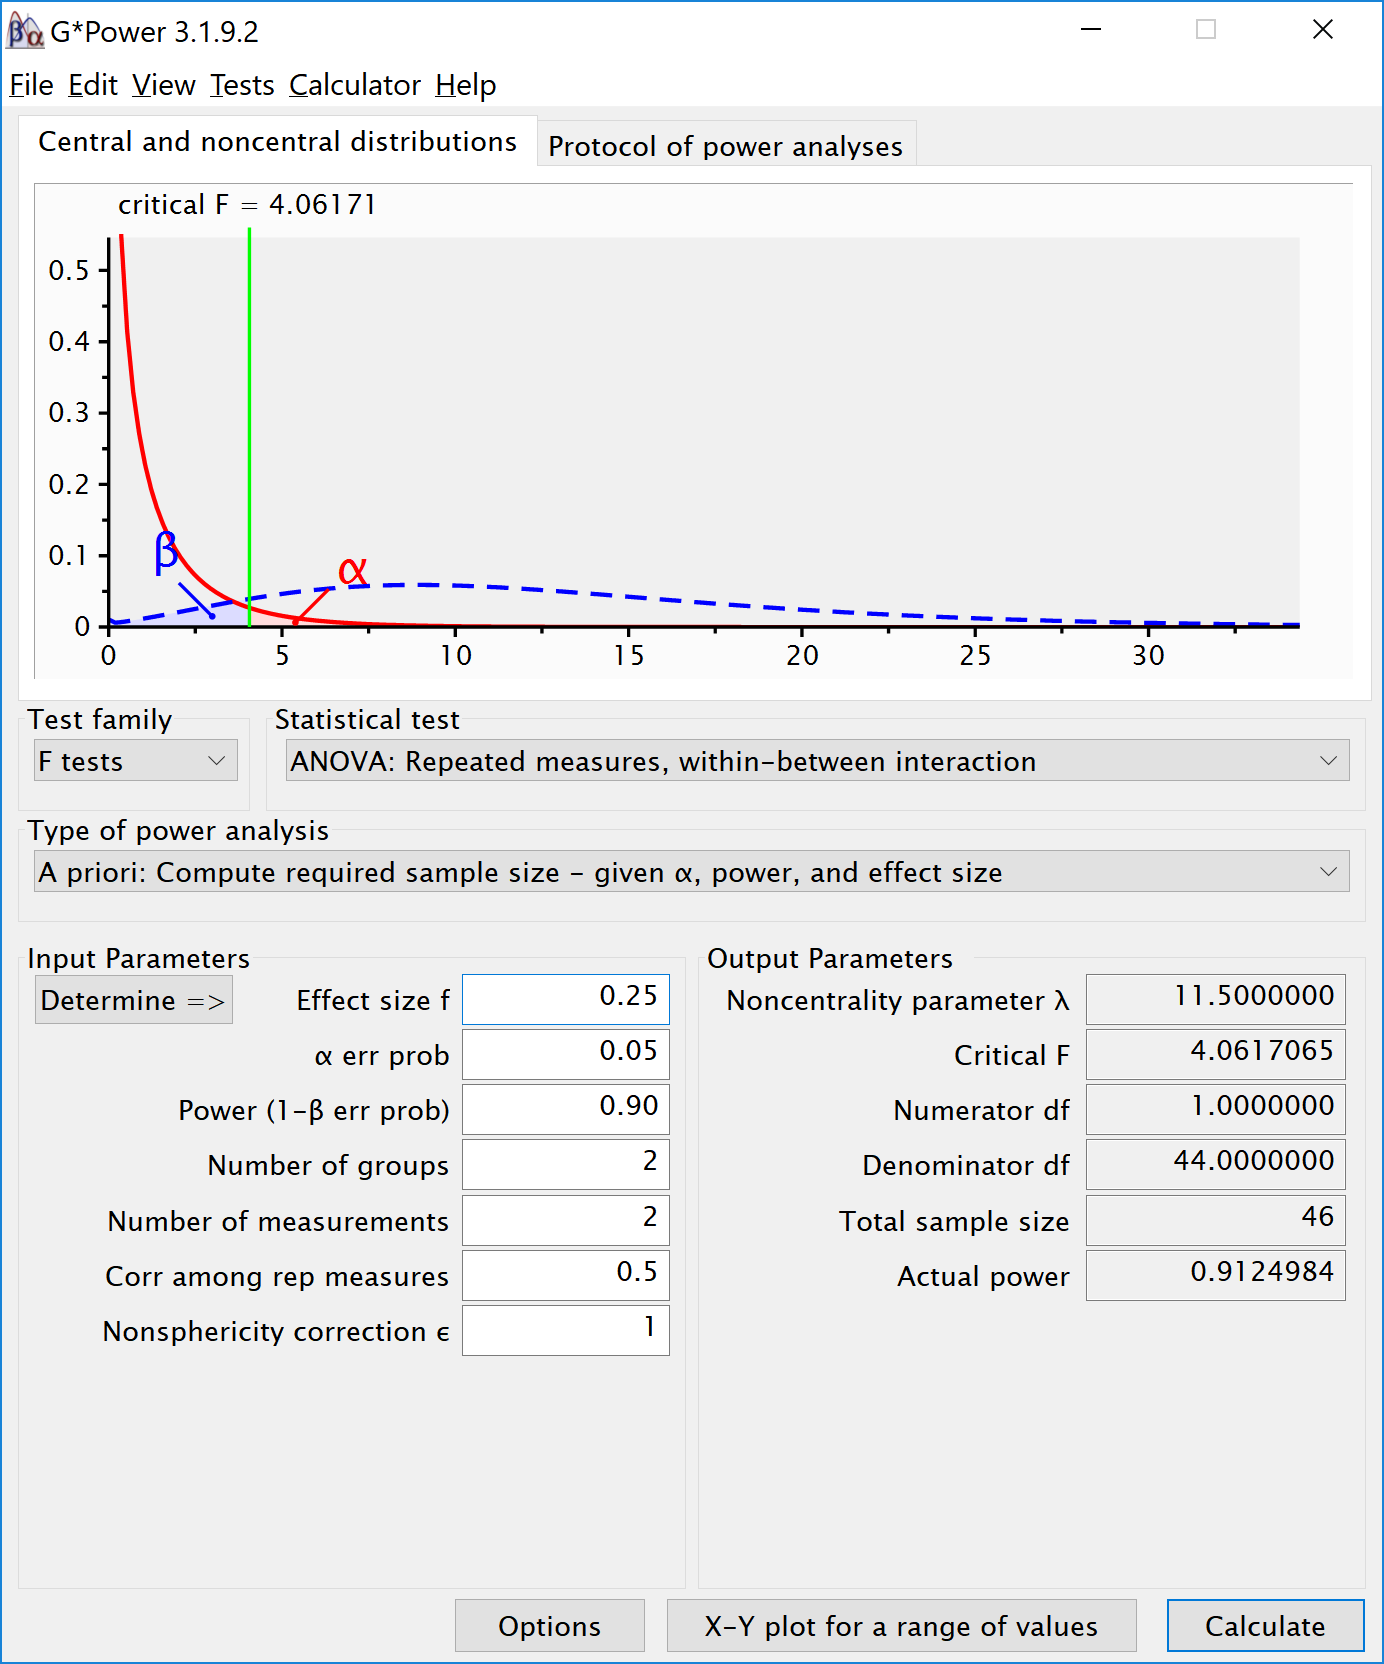
\includegraphics{screenshots/gpower_5.png}
\newpage

Now, we can repeat the process in \texttt{Superpower}.

\begin{Shaded}
\begin{Highlighting}[]
\NormalTok{mu <-}\StringTok{ }\KeywordTok{c}\NormalTok{(}\OperatorTok{-}\FloatTok{0.25}\NormalTok{, }\FloatTok{0.25}\NormalTok{, }\FloatTok{0.25}\NormalTok{,}\OperatorTok{-}\FloatTok{0.25}\NormalTok{)}
\NormalTok{n <-}\StringTok{ }\DecValTok{23}
\NormalTok{sd <-}\StringTok{ }\DecValTok{1}
\NormalTok{r <-}\StringTok{ }\FloatTok{0.5}
\NormalTok{string =}\StringTok{ "2w*2b"}
\NormalTok{alpha_level <-}\StringTok{ }\FloatTok{0.05}
\NormalTok{labelnames =}\StringTok{ }\KeywordTok{c}\NormalTok{(}\StringTok{"age"}\NormalTok{, }\StringTok{"old"}\NormalTok{, }\StringTok{"young"}\NormalTok{, }\StringTok{"color"}\NormalTok{, }\StringTok{"blue"}\NormalTok{, }\StringTok{"red"}\NormalTok{)}
\NormalTok{design_result <-}\StringTok{ }\KeywordTok{ANOVA_design}\NormalTok{(}
\DataTypeTok{design =}\NormalTok{ string,}
\DataTypeTok{n =}\NormalTok{ n,}
\DataTypeTok{mu =}\NormalTok{ mu,}
\DataTypeTok{sd =}\NormalTok{ sd,}
\DataTypeTok{r =}\NormalTok{ r,}
\DataTypeTok{labelnames =}\NormalTok{ labelnames}
\NormalTok{)}
\end{Highlighting}
\end{Shaded}

\begin{Shaded}
\begin{Highlighting}[]
\NormalTok{simulation_result <-}\StringTok{ }\KeywordTok{ANOVA_power}\NormalTok{(design_result, }
                                 \DataTypeTok{alpha_level =}\NormalTok{ alpha_level, }
                                 \DataTypeTok{nsims =}\NormalTok{ nsims,}
                                 \DataTypeTok{verbose =} \OtherTok{FALSE}\NormalTok{)}
\end{Highlighting}
\end{Shaded}

\begin{table}[!h]

\caption{\label{tab:unnamed-chunk-196}Simulated ANOVA Result}
\centering
\begin{tabular}{l|r|r}
\hline
  & power & effect\_size\\
\hline
anova\_color & 4.45 & 0.0215448\\
\hline
anova\_age & 5.29 & 0.0221193\\
\hline
anova\_color:age & 91.26 & 0.2155901\\
\hline
\end{tabular}
\end{table}

\begin{Shaded}
\begin{Highlighting}[]
\NormalTok{exact_result <-}\StringTok{ }\KeywordTok{ANOVA_exact}\NormalTok{(design_result,}
                            \DataTypeTok{alpha_level =}\NormalTok{ alpha_level,}
                            \DataTypeTok{verbose =} \OtherTok{FALSE}\NormalTok{)}
\end{Highlighting}
\end{Shaded}

\begin{table}[!h]

\caption{\label{tab:unnamed-chunk-198}Exact ANOVA Result}
\centering
\begin{tabular}{l|r|r|r|r}
\hline
  & power & partial\_eta\_squared & cohen\_f & non\_centrality\\
\hline
color & 5.00000 & 0.0000000 & 0.0000000 & 0.0\\
\hline
age & 5.00000 & 0.0000000 & 0.0000000 & 0.0\\
\hline
color:age & 91.24984 & 0.2072072 & 0.5112374 & 11.5\\
\hline
\end{tabular}
\end{table}

\newpage

Now, we can simulate the same two-way ANOVA but increasing the correlation to r=0.7.

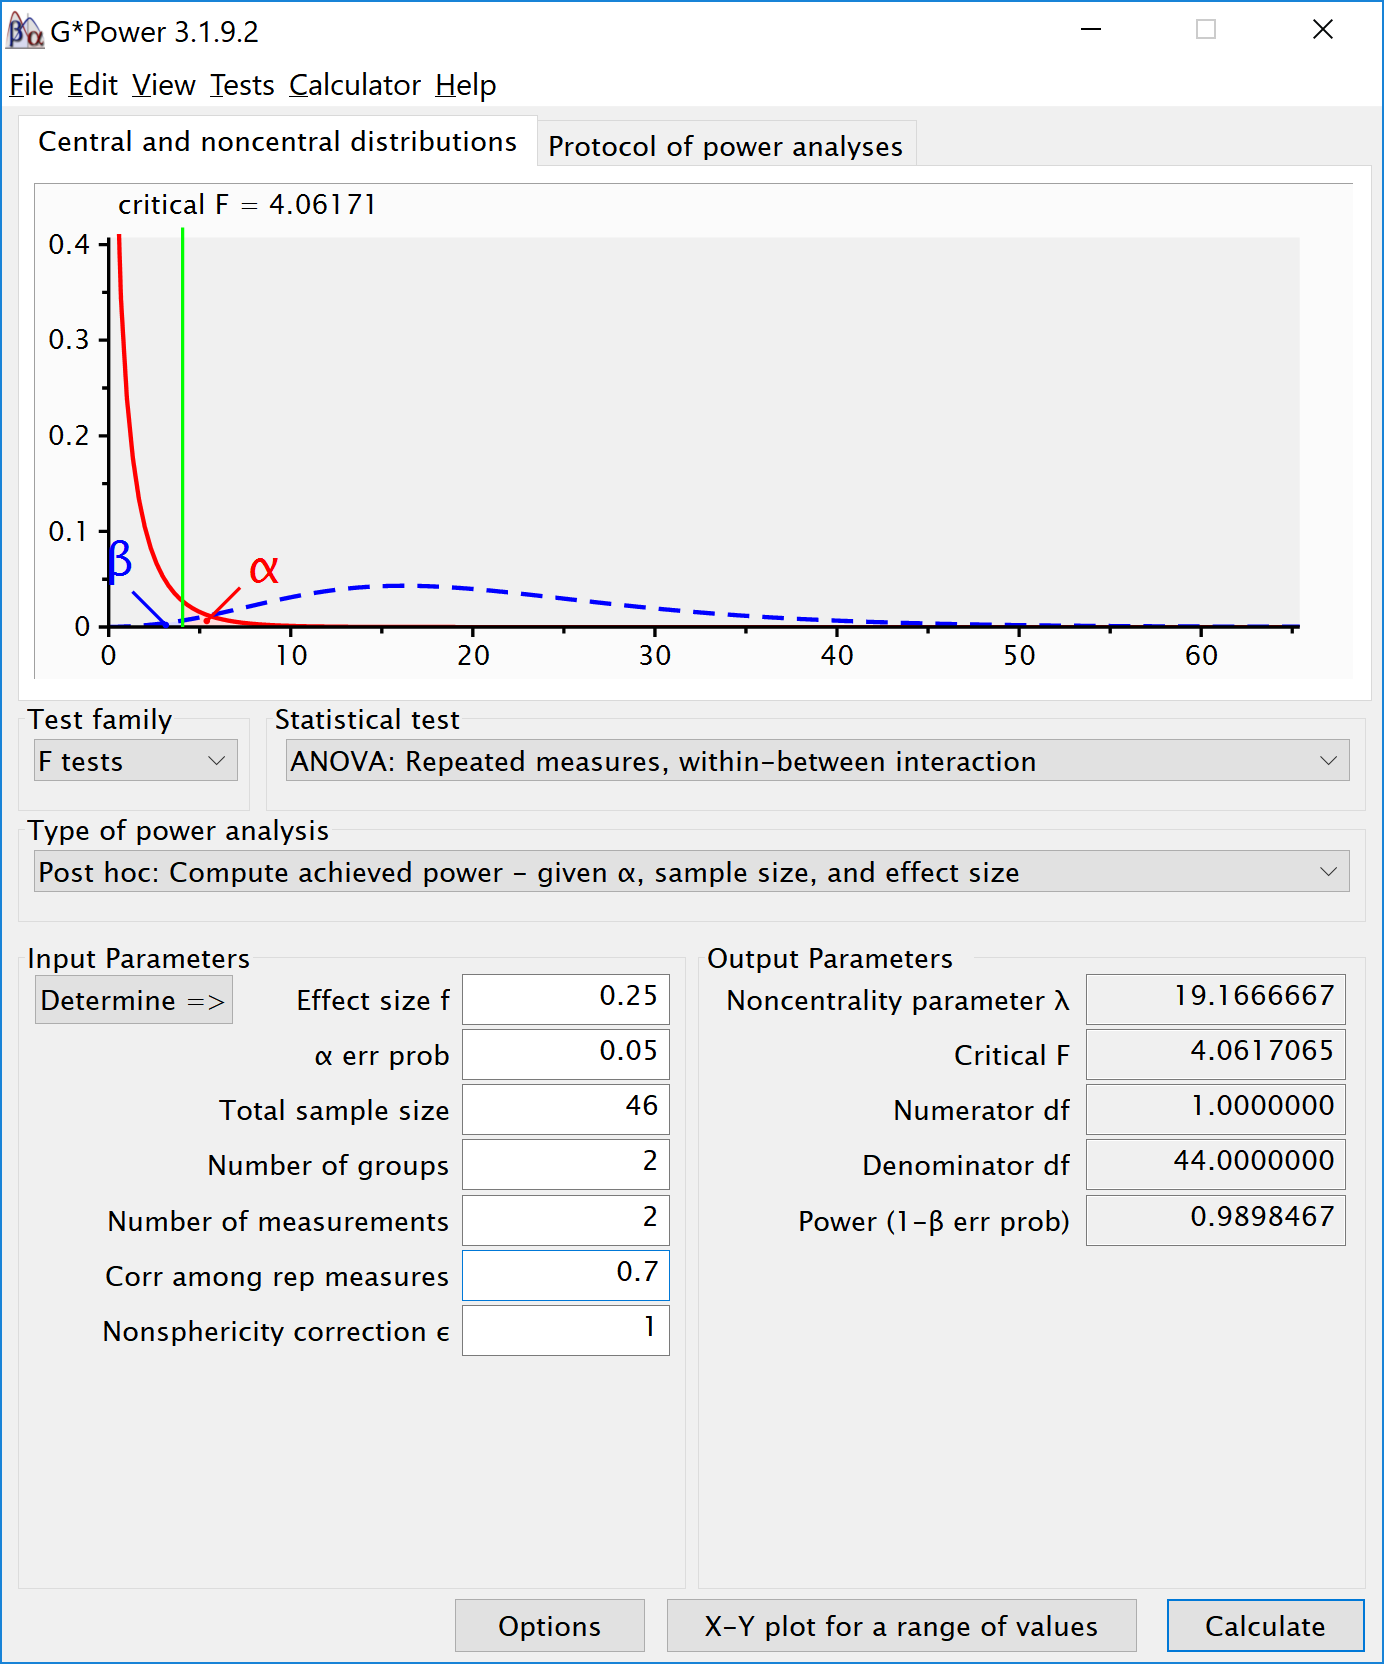
\includegraphics{screenshots/gpower_6.png}
\newpage

\begin{Shaded}
\begin{Highlighting}[]
\NormalTok{mu <-}\StringTok{ }\KeywordTok{c}\NormalTok{(}\OperatorTok{-}\FloatTok{0.25}\NormalTok{, }\FloatTok{0.25}\NormalTok{, }\FloatTok{0.25}\NormalTok{, }\FloatTok{-0.25}\NormalTok{)}
\NormalTok{n <-}\StringTok{ }\DecValTok{23}
\NormalTok{sd <-}\StringTok{ }\DecValTok{1}
\NormalTok{r <-}\StringTok{ }\FloatTok{0.7}
\NormalTok{string =}\StringTok{ "2w*2b"}
\NormalTok{alpha_level <-}\StringTok{ }\FloatTok{0.05}
\NormalTok{labelnames =}\StringTok{ }\KeywordTok{c}\NormalTok{(}\StringTok{"age"}\NormalTok{, }\StringTok{"old"}\NormalTok{, }\StringTok{"young"}\NormalTok{, }\StringTok{"color"}\NormalTok{, }\StringTok{"blue"}\NormalTok{, }\StringTok{"red"}\NormalTok{)}
\NormalTok{design_result <-}\StringTok{ }\KeywordTok{ANOVA_design}\NormalTok{(}\DataTypeTok{design =}\NormalTok{ string,}
                              \DataTypeTok{n =}\NormalTok{ n, }
                              \DataTypeTok{mu =}\NormalTok{ mu, }
                              \DataTypeTok{sd =}\NormalTok{ sd, }
                              \DataTypeTok{r =}\NormalTok{ r, }
                              \DataTypeTok{labelnames =}\NormalTok{ labelnames)}
\end{Highlighting}
\end{Shaded}

\begin{Shaded}
\begin{Highlighting}[]
\NormalTok{simulation_result <-}\StringTok{ }\KeywordTok{ANOVA_power}\NormalTok{(design_result, }
                                 \DataTypeTok{alpha_level =}\NormalTok{ alpha_level, }
                                 \DataTypeTok{nsims =}\NormalTok{ nsims,}
                                 \DataTypeTok{verbose =} \OtherTok{FALSE}\NormalTok{)}
\end{Highlighting}
\end{Shaded}

\begin{table}[!h]

\caption{\label{tab:unnamed-chunk-201}Simulated ANOVA Result}
\centering
\begin{tabular}{l|r|r}
\hline
  & power & effect\_size\\
\hline
anova\_color & 4.93 & 0.0220656\\
\hline
anova\_age & 4.85 & 0.0224569\\
\hline
anova\_color:age & 99.00 & 0.3081551\\
\hline
\end{tabular}
\end{table}

\begin{Shaded}
\begin{Highlighting}[]
\NormalTok{exact_result <-}\StringTok{ }\KeywordTok{ANOVA_exact}\NormalTok{(design_result,}
                            \DataTypeTok{alpha_level =}\NormalTok{ alpha_level,}
                            \DataTypeTok{verbose =} \OtherTok{FALSE}\NormalTok{)}
\end{Highlighting}
\end{Shaded}

\begin{table}[!h]

\caption{\label{tab:unnamed-chunk-203}Exact ANOVA Result}
\centering
\begin{tabular}{l|r|r|r|r}
\hline
  & power & partial\_eta\_squared & cohen\_f & non\_centrality\\
\hline
color & 5.00000 & 0.0000000 & 0.0000000 & 0.00000\\
\hline
age & 5.00000 & 0.0000000 & 0.0000000 & 0.00000\\
\hline
color:age & 98.98467 & 0.3034301 & 0.6600046 & 19.16667\\
\hline
\end{tabular}
\end{table}

\newpage

\hypertarget{complex-mixed-designs}{%
\section{Complex Mixed Designs}\label{complex-mixed-designs}}

Now, we are to the most complicated calculations. Similiar to the simple one-way repeated measures ANOVA, a mixed ANOVA assumes sphercity. Therefore, in most situations a multivariate approach, MANOVA, is recommended \citep{maxwell_designing_2004}. To our knowledge, the only program that can accurately calculate power for mixed designs with greater than 2 levels is SAS's \texttt{PROC\ GLMPOWER} \citep{SASglmpower}. The procedure utilizes approximate analytical solutions derived by \citet{muller1984practical} and \citet{o1999pragmatic}. According to the documentation, these analytical solutions are very accurate for all but small N situations (sorry exercise scientists!). Eventually, this chapter will document the analytical solution in a step-by-step fashion, but for the time being we will just directly compare \texttt{Superpower} to \texttt{GLMPOWER} from a few examples provided by SAS.

\hypertarget{b3w-design}{%
\subsection{2b*3w Design}\label{b3w-design}}

Here we will use a modified example from \citet{SASglmpower} pg. 3739. In this hypothetical experiment Suppose you are planning an experiment to study the growth of two varieties of flowers over the course of 3 weeks. The planned data analysis is a two-way ANOVA with flower height as the outcome and a model consisting of the effects of time, flower variety, and their interaction.

First we can set up the dataframe in SAS. This is similiar to the \texttt{mu} command in \texttt{ANOVA\_design}.

\begin{Shaded}
\begin{Highlighting}[]
\NormalTok{data Exemplary2;}
\NormalTok{input variety Height1 Height2 Height3;}
\NormalTok{datalines;}
\DecValTok{1} \DecValTok{14} \DecValTok{16} \DecValTok{21}
\DecValTok{2} \DecValTok{10} \DecValTok{15} \DecValTok{16}
\NormalTok{;}
\end{Highlighting}
\end{Shaded}

We can now solve for power in \texttt{PROC\ GLMPOWER}. In this case, we set up a multivariate repeated measures model, with a total of 40 flowers (20 per variety). We also setup the within-factor correlations with the CORRS command.

\begin{Shaded}
\begin{Highlighting}[]
\NormalTok{proc glmpower data=Exemplary2;}
\NormalTok{class Variety Exposure;}
\NormalTok{model Height1 Height2 Height3 =}\StringTok{ }\NormalTok{Variety;}
\NormalTok{repeated Time contrast;}
\NormalTok{power}
\NormalTok{mtest =}\StringTok{ }\NormalTok{pt}
\NormalTok{stddev =}\StringTok{ }\DecValTok{5}
\NormalTok{ntotal =}\StringTok{ }\DecValTok{40}
\NormalTok{power =}\StringTok{ }\NormalTok{.}
\KeywordTok{MATRIX}\NormalTok{(}\StringTok{"MyCorrs"}\NormalTok{)=}\StringTok{ }\NormalTok{(.}\DecValTok{75}\NormalTok{,}
                    \FloatTok{0.5625}\NormalTok{,.}\DecValTok{75}\NormalTok{)}
\NormalTok{CORRS=}\StringTok{ "MyCorrs"}\NormalTok{;}
\NormalTok{run;}
\end{Highlighting}
\end{Shaded}

The power analysis results then get printed to the SAS ouput page.

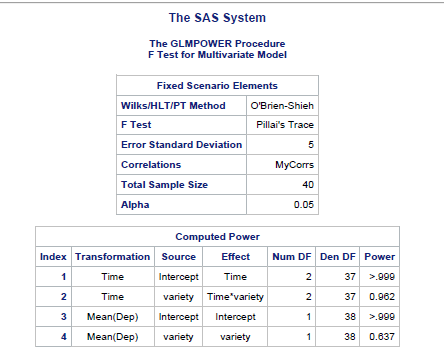
\includegraphics{screenshots/sas_2x3repeated.png}

Now let's replicate this in \texttt{R} with \texttt{Superpower}. First, we setup the same design with \texttt{ANOVA\_design}.

\begin{Shaded}
\begin{Highlighting}[]
\NormalTok{cor_}\DecValTok{1}\NormalTok{ <-}\StringTok{ }\KeywordTok{matrix}\NormalTok{(}\KeywordTok{c}\NormalTok{(}\DecValTok{1}\NormalTok{, }\FloatTok{.75}\NormalTok{, }\FloatTok{.5625}\NormalTok{,}
                  \FloatTok{.75}\NormalTok{, }\DecValTok{1}\NormalTok{, }\FloatTok{.75}\NormalTok{,}
                  \FloatTok{.5625}\NormalTok{, }\FloatTok{.75}\NormalTok{, }\DecValTok{1}\NormalTok{), }\DataTypeTok{nrow=}\DecValTok{3}\NormalTok{)}

\NormalTok{cor_}\DecValTok{2}\NormalTok{ <-}\StringTok{ }\NormalTok{cor_}\DecValTok{1}\OperatorTok{*}\DecValTok{0}

\NormalTok{rho_mat <-}\StringTok{ }\KeywordTok{cbind}\NormalTok{(}\KeywordTok{rbind}\NormalTok{(cor_}\DecValTok{1}\NormalTok{,cor_}\DecValTok{2}\NormalTok{),}
                      \KeywordTok{rbind}\NormalTok{(cor_}\DecValTok{2}\NormalTok{,cor_}\DecValTok{1}\NormalTok{))}

\NormalTok{design_result <-}\StringTok{ }\KeywordTok{ANOVA_design}\NormalTok{(}\StringTok{"2b*3w"}\NormalTok{,}
                              \DataTypeTok{n =} \DecValTok{20}\NormalTok{,}
                              \DataTypeTok{sd =} \DecValTok{5}\NormalTok{,}
                              \DataTypeTok{mu =} \KeywordTok{c}\NormalTok{(}\DecValTok{14}\NormalTok{, }\DecValTok{16}\NormalTok{, }\DecValTok{21}\NormalTok{,}
                                     \DecValTok{10}\NormalTok{, }\DecValTok{15}\NormalTok{, }\DecValTok{16}\NormalTok{),}
                              \DataTypeTok{r =}\NormalTok{ rho_mat,}
                              \DataTypeTok{labelnames =} \KeywordTok{c}\NormalTok{(}\StringTok{"VARIETY"}\NormalTok{, }
                                             \StringTok{"type1"}\NormalTok{, }\StringTok{"type2"}\NormalTok{,}
                                             \StringTok{"TIME"}\NormalTok{, }
                                             \StringTok{"height1"}\NormalTok{, }\StringTok{"height2"}\NormalTok{, }
                                             \StringTok{"height3"}\NormalTok{),}
                              \DataTypeTok{plot =} \OtherTok{TRUE}\NormalTok{)}
\end{Highlighting}
\end{Shaded}

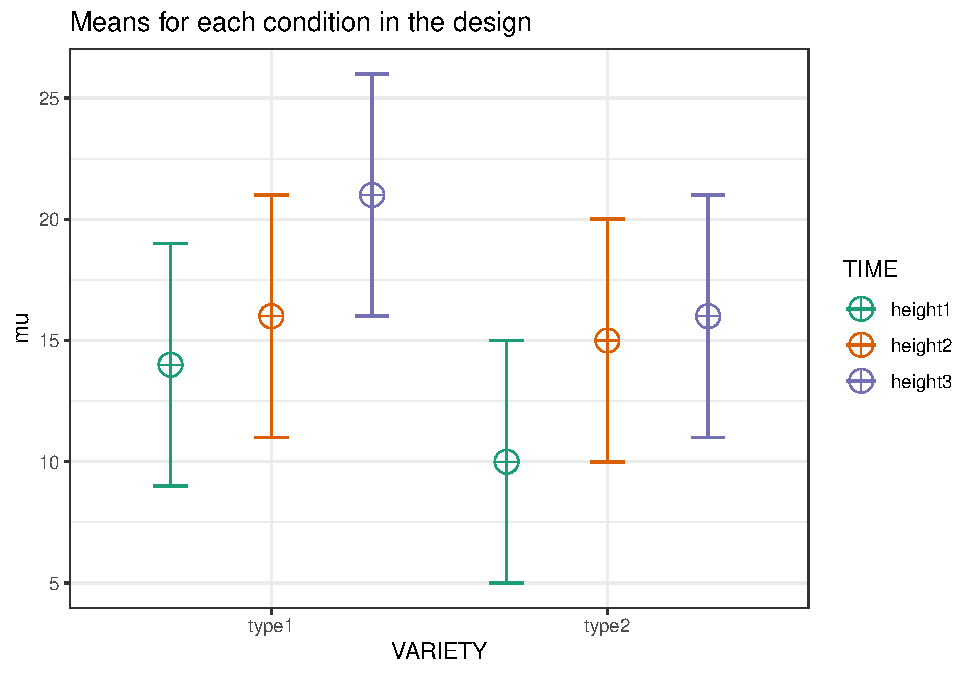
\includegraphics{SuperpowerValidation_files/figure-latex/unnamed-chunk-206-1.pdf}

\begin{Shaded}
\begin{Highlighting}[]
\NormalTok{exact_result <-}\StringTok{ }\KeywordTok{ANOVA_exact}\NormalTok{(design_result, }\DataTypeTok{verbose =} \OtherTok{FALSE}\NormalTok{,}
                            \DataTypeTok{correction =} \StringTok{"none"}\NormalTok{,}
                            \DataTypeTok{alpha_level =} \FloatTok{.05}\NormalTok{)}
\end{Highlighting}
\end{Shaded}

\begin{table}[!h]

\caption{\label{tab:unnamed-chunk-208}MANOVA Result}
\centering
\begin{tabular}{l|r|r|r|r}
\hline
  & power & partial\_eta\_squared & cohen\_f & non\_centrality\\
\hline
VARIETY & 63.65566 & 0.1287208 & 0.3843667 & 5.614035\\
\hline
TIME & 100.00000 & 0.5877929 & 1.1941377 & 108.373333\\
\hline
VARIETY:TIME & 84.08029 & 0.1273729 & 0.3820535 & 11.093333\\
\hline
\end{tabular}
\end{table}

You will notice a small discrepancy between the two power estimates for the main effect of variety. This difference is due to the analytical solutions problems with small sample sizes. You will see in the example below that the results match when the total sample size is much greater.

\hypertarget{b4w-design}{%
\subsection{2b*4w Design}\label{b4w-design}}

Now we move onto the example from pg 3794 of \citet{SASglmpower}.

As stated in the manual:

\begin{quote}
Logan, Baron, and Kohout (1995) and Guo et al.~(2013) study the effect of a dental intervention on the
memory of pain after root canal therapy. The intervention is a sensory focus strategy, in which patients are
instructed to pay attention only to the physical sensations in their mouth during the root canal procedure.
Suppose you are interested in the long-term effects of this sensory focus intervention, because avoidance
behavior has been shown to build along with memory of pain. You are planning a study to compare
sensory focus to standard of care over a period of a year, asking patients to self-report their memory of pain
immediately after the procedure and then again at 1 week, 6 months, and 12 months. You use a scale from 0
(no pain remembered) to 5 (maximum pain remembered).
\end{quote}

This makes it a \texttt{2b*4w} design with treatment as a between subjects factor, with two levels (sensory focus versus standard of care), and time as a within-subject factor is time, with four levels (0, 1, 26, and 52 weeks). In this case, we differ from \citet{SASglmpower} and we will solve for power with a sample size of 300 per group (600 total) with an alpha of \texttt{.01}. In addition, we want to see what the impact of chaning the common standard deviation will have on power.

So in SAS we set up the data.

\begin{Shaded}
\begin{Highlighting}[]
\NormalTok{data Pain;}
\NormalTok{input Treatment }\OperatorTok{$}\StringTok{ }\NormalTok{PainMem0 PainMem1Wk PainMem6Mo PainMem12Mo;}
\NormalTok{datalines;}
\NormalTok{SensoryFocus }\FloatTok{2.40} \FloatTok{2.38} \FloatTok{2.05} \FloatTok{1.90}
\NormalTok{StandardOfCare }\FloatTok{2.40} \FloatTok{2.39} \FloatTok{2.36} \FloatTok{2.30}
\NormalTok{;}
\end{Highlighting}
\end{Shaded}

Then we can run the analysis in SAS. Note that in the example \citet{SASglmpower} are assuming a linear exponential covariance matrix, which we can mimic in \texttt{R}.

\begin{Shaded}
\begin{Highlighting}[]
\NormalTok{proc glmpower data=Pain;}
\NormalTok{class Treatment;}
\NormalTok{model PainMem0 PainMem1Wk PainMem6Mo PainMem12Mo =}\StringTok{ }\NormalTok{Treatment;}
\NormalTok{repeated Time contrast;}
\NormalTok{power}
\NormalTok{mtest =}\StringTok{ }\NormalTok{pt }
\NormalTok{alpha =}\StringTok{ }\FloatTok{0.01}
\NormalTok{power =}\StringTok{ }\NormalTok{.}
\NormalTok{ntotal =}\StringTok{ }\DecValTok{600}
\NormalTok{stddev =}\StringTok{ }\FloatTok{0.92} \FloatTok{1.04}
\KeywordTok{matrix}\NormalTok{ (}\StringTok{"PainCorr"}\NormalTok{) =}\StringTok{ }\KeywordTok{lear}\NormalTok{(}\FloatTok{0.6}\NormalTok{, }\FloatTok{0.8}\NormalTok{, }\DecValTok{4}\NormalTok{, }\DecValTok{0} \DecValTok{1} \DecValTok{26} \DecValTok{52}\NormalTok{)}
\NormalTok{corrmat =}\StringTok{ "PainCorr"}\NormalTok{;}
\NormalTok{run;}
\NormalTok{quit;}
\end{Highlighting}
\end{Shaded}

This produces a table with the result for a power analysis with 2 different common standard deviations.

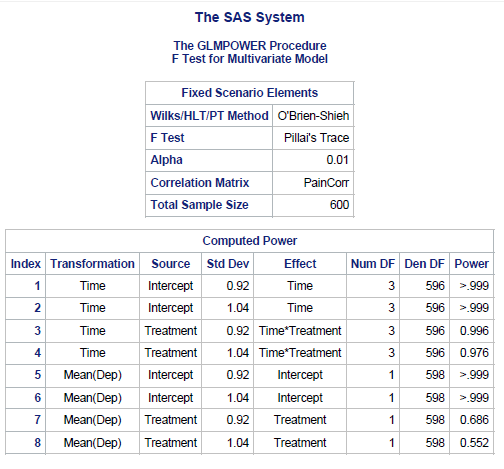
\includegraphics{screenshots/sas_pain.png}

We then replicate in \texttt{R}, first by setting up the ``lear'' correlation matrix.

\begin{Shaded}
\begin{Highlighting}[]
\NormalTok{cor_}\DecValTok{1}\NormalTok{ <-}\StringTok{ }\KeywordTok{matrix}\NormalTok{(}\KeywordTok{c}\NormalTok{(}\DecValTok{1}\NormalTok{,.}\DecValTok{6}\NormalTok{,.}\DecValTok{491}\NormalTok{,.}\DecValTok{399}\NormalTok{,}
                  \FloatTok{.6}\NormalTok{,}\DecValTok{1}\NormalTok{,.}\DecValTok{495}\NormalTok{,.}\DecValTok{402}\NormalTok{,}
                  \FloatTok{.491}\NormalTok{,.}\DecValTok{495}\NormalTok{,}\DecValTok{1}\NormalTok{,.}\DecValTok{491}\NormalTok{,}
                  \FloatTok{.399}\NormalTok{,.}\DecValTok{402}\NormalTok{,.}\DecValTok{491}\NormalTok{,}\DecValTok{1}\NormalTok{), }\DataTypeTok{nrow=}\DecValTok{4}\NormalTok{)}

\NormalTok{cor_}\DecValTok{2}\NormalTok{ <-}\StringTok{ }\NormalTok{cor_}\DecValTok{1}\OperatorTok{*}\DecValTok{0}

\NormalTok{pain_cor_mat <-}\StringTok{ }\KeywordTok{cbind}\NormalTok{(}\KeywordTok{rbind}\NormalTok{(cor_}\DecValTok{1}\NormalTok{,cor_}\DecValTok{2}\NormalTok{),}
                      \KeywordTok{rbind}\NormalTok{(cor_}\DecValTok{2}\NormalTok{,cor_}\DecValTok{1}\NormalTok{))}

\NormalTok{design_result <-}\StringTok{ }\KeywordTok{ANOVA_design}\NormalTok{(}\StringTok{"2b*4w"}\NormalTok{,}
                              \DataTypeTok{n =} \DecValTok{300}\NormalTok{,}
                              \DataTypeTok{mu =} \KeywordTok{c}\NormalTok{(}\FloatTok{2.4}\NormalTok{, }\FloatTok{2.38}\NormalTok{, }\FloatTok{2.05}\NormalTok{, }\FloatTok{1.90}\NormalTok{,}
                                     \FloatTok{2.4}\NormalTok{, }\FloatTok{2.39}\NormalTok{, }\FloatTok{2.36}\NormalTok{, }\FloatTok{2.30}\NormalTok{),}
                              \DataTypeTok{sd =} \FloatTok{.92}\NormalTok{,}
                              \DataTypeTok{r =}\NormalTok{ pain_cor_mat,}
                              \DataTypeTok{labelnames =} \KeywordTok{c}\NormalTok{(}\StringTok{"Treatment"}\NormalTok{, }\StringTok{"sensory"}\NormalTok{, }\StringTok{"standard"}\NormalTok{,}
                                             \StringTok{"TIME"}\NormalTok{, }\StringTok{"t1"}\NormalTok{, }\StringTok{"t2"}\NormalTok{, }\StringTok{"t3"}\NormalTok{, }\StringTok{"t4"}\NormalTok{),}
                              \DataTypeTok{plot =} \OtherTok{TRUE}\NormalTok{)}
\end{Highlighting}
\end{Shaded}

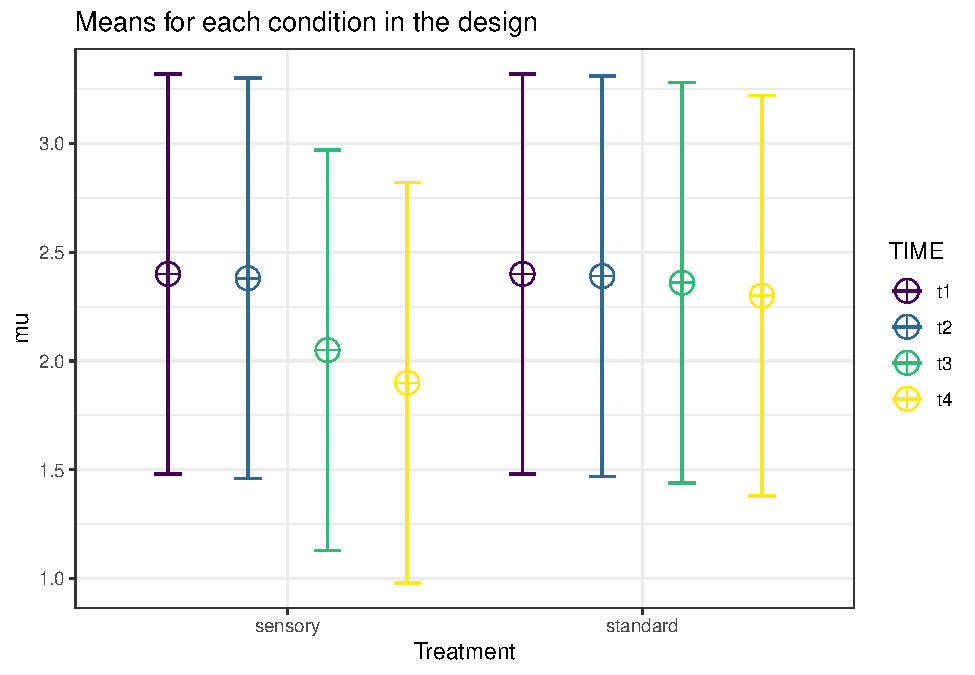
\includegraphics{SuperpowerValidation_files/figure-latex/mixed_multivariate_1-1.pdf}

\begin{Shaded}
\begin{Highlighting}[]
\NormalTok{exact_result <-}\StringTok{ }\KeywordTok{ANOVA_exact}\NormalTok{(design_result, }\DataTypeTok{verbose =} \OtherTok{FALSE}\NormalTok{,}
                            \DataTypeTok{alpha_level =} \FloatTok{.01}\NormalTok{)}
\end{Highlighting}
\end{Shaded}

\begin{table}[!h]

\caption{\label{tab:unnamed-chunk-211}Simulated MANOVA Result}
\centering
\begin{tabular}{l|r|r|r|r}
\hline
  & power & pillai\_trace & cohen\_f & non\_centrality\\
\hline
(Intercept) & 100.00000 & 0.9094197 & 3.1685838 & 6003.874016\\
\hline
Treatment & 68.59334 & 0.0155032 & 0.1254885 & 9.416918\\
\hline
TIME & 99.99995 & 0.0998664 & 0.3330858 & 66.123912\\
\hline
Treatment:TIME & 99.55718 & 0.0531965 & 0.2370344 & 33.486447\\
\hline
\end{tabular}
\end{table}

\begin{Shaded}
\begin{Highlighting}[]
\NormalTok{design_result <-}\StringTok{ }\KeywordTok{ANOVA_design}\NormalTok{(}\StringTok{"2b*4w"}\NormalTok{,}
                              \DataTypeTok{n =} \DecValTok{300}\NormalTok{,}
                              \DataTypeTok{mu =} \KeywordTok{c}\NormalTok{(}\FloatTok{2.4}\NormalTok{, }\FloatTok{2.38}\NormalTok{, }\FloatTok{2.05}\NormalTok{, }\FloatTok{1.90}\NormalTok{,}
                                     \FloatTok{2.4}\NormalTok{, }\FloatTok{2.39}\NormalTok{, }\FloatTok{2.36}\NormalTok{, }\FloatTok{2.30}\NormalTok{),}
                              \DataTypeTok{sd =} \FloatTok{1.04}\NormalTok{,}
                              \DataTypeTok{r =}\NormalTok{ pain_cor_mat,}
                              \DataTypeTok{labelnames =} \KeywordTok{c}\NormalTok{(}\StringTok{"Treatment"}\NormalTok{, }\StringTok{"sensory"}\NormalTok{, }\StringTok{"standard"}\NormalTok{,}
                                             \StringTok{"TIME"}\NormalTok{, }\StringTok{"t1"}\NormalTok{, }\StringTok{"t2"}\NormalTok{, }\StringTok{"t3"}\NormalTok{, }\StringTok{"t4"}\NormalTok{),}
                              \DataTypeTok{plot =} \OtherTok{TRUE}\NormalTok{)}
\end{Highlighting}
\end{Shaded}

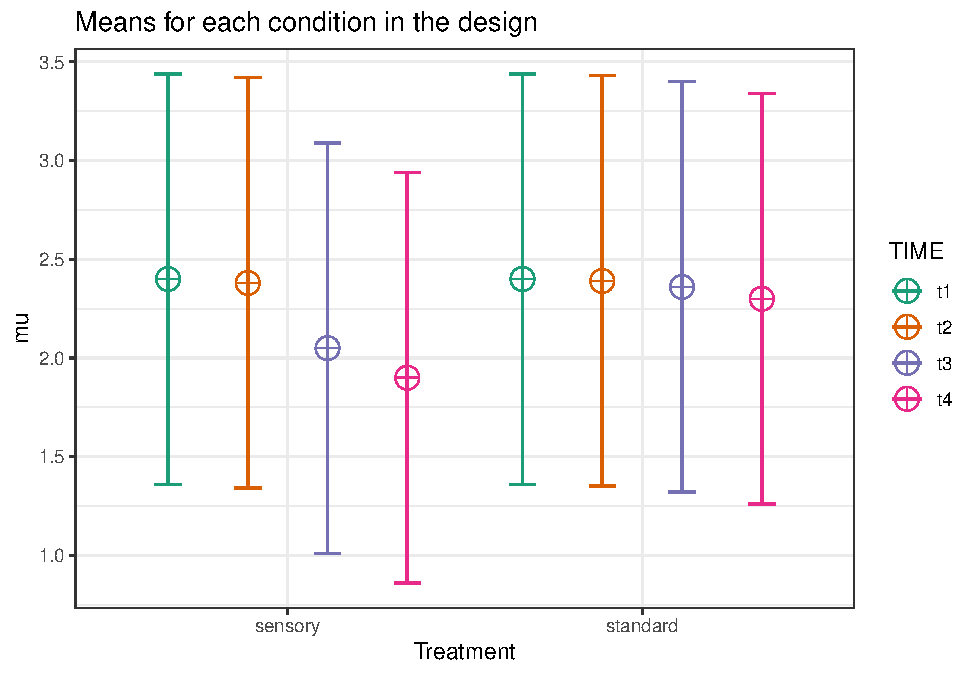
\includegraphics{SuperpowerValidation_files/figure-latex/unnamed-chunk-212-1.pdf}

\begin{Shaded}
\begin{Highlighting}[]
\NormalTok{exact_result <-}\StringTok{ }\KeywordTok{ANOVA_exact}\NormalTok{(design_result, }\DataTypeTok{verbose =} \OtherTok{FALSE}\NormalTok{,}
                            \DataTypeTok{alpha_level =} \FloatTok{.01}\NormalTok{)}
\end{Highlighting}
\end{Shaded}

\begin{table}[!h]

\caption{\label{tab:unnamed-chunk-213}Simulated MANOVA Result}
\centering
\begin{tabular}{l|r|r|r|r}
\hline
  & power & pillai\_trace & cohen\_f & non\_centrality\\
\hline
(Intercept) & 100.00000 & 0.8870909 & 2.8029779 & 4698.297861\\
\hline
Treatment & 55.22151 & 0.0121730 & 0.1110090 & 7.369156\\
\hline
TIME & 99.99672 & 0.0798847 & 0.2946528 & 51.744895\\
\hline
Treatment:TIME & 97.55110 & 0.0421158 & 0.2096843 & 26.204631\\
\hline
\end{tabular}
\end{table}

As we can see, the results for this analysis match SAS perfectly.

\hypertarget{power-for-three-way-interactions}{%
\chapter{Power for Three-way Interactions}\label{power-for-three-way-interactions}}

There are almost no software solutions that allow researchers to perform power anaysis for more complex designs. Through simulation, it is relatively straightforward to examine the power for designs with multiple factors with many levels.

Let's start with a 2x2x2 between-subjects design. We collect 50 participants in each between participant condition (so 400 participants in total - \(50(n)\times2(levels)\times2(levels)\times2(levels)= 400\)).

\begin{Shaded}
\begin{Highlighting}[]
\CommentTok{# With 2x2x2 designs, }
\CommentTok{# the names for paired comparisons can become very long. }
\CommentTok{# So here I abbreviate terms: }
\CommentTok{#   Size, Color, and Cognitive Load, have values:}
\CommentTok{# b = big, s = small, g = green, }
\CommentTok{# r = red, pres = present, abs = absent.  }
\NormalTok{labelnames <-}\StringTok{ }\KeywordTok{c}\NormalTok{(}\StringTok{"Size"}\NormalTok{, }\StringTok{"b"}\NormalTok{, }\StringTok{"s"}\NormalTok{, }\StringTok{"Color"}\NormalTok{, }\StringTok{"g"}\NormalTok{, }\StringTok{"r"}\NormalTok{, }
                \StringTok{"Load"}\NormalTok{, }\StringTok{"pres"}\NormalTok{, }\StringTok{"abs"}\NormalTok{) }\CommentTok{#}
\NormalTok{design_result <-}\StringTok{ }\KeywordTok{ANOVA_design}\NormalTok{(}\DataTypeTok{design =} \StringTok{"2b*2b*2b"}\NormalTok{, }
                              \CommentTok{#sample size per group }
                              \DataTypeTok{n =} \DecValTok{50}\NormalTok{, }
                              \CommentTok{#pattern of means}
                              \DataTypeTok{mu =} \KeywordTok{c}\NormalTok{(}\DecValTok{2}\NormalTok{, }\DecValTok{2}\NormalTok{, }\DecValTok{6}\NormalTok{, }\DecValTok{1}\NormalTok{, }\DecValTok{6}\NormalTok{, }\DecValTok{6}\NormalTok{, }\DecValTok{1}\NormalTok{, }\DecValTok{8}\NormalTok{), }
                              \DataTypeTok{sd =} \DecValTok{10}\NormalTok{, }\CommentTok{#standard deviation}
                              \DataTypeTok{labelnames =}\NormalTok{ labelnames) }
\end{Highlighting}
\end{Shaded}

\begin{Shaded}
\begin{Highlighting}[]
\NormalTok{simulation_result <-}\StringTok{ }\KeywordTok{ANOVA_power}\NormalTok{(design_result, }
                                 \DataTypeTok{alpha_level =}\NormalTok{ alpha_level, }
                                 \DataTypeTok{nsims =}\NormalTok{ nsims,}
                                 \DataTypeTok{verbose =} \OtherTok{FALSE}\NormalTok{)}
\end{Highlighting}
\end{Shaded}

\begin{table}[!h]

\caption{\label{tab:unnamed-chunk-216}Simulated ANOVA Result}
\centering
\begin{tabular}{l|r|r}
\hline
  & power & effect\_size\\
\hline
anova\_Size & 70.17 & 0.0181513\\
\hline
anova\_Color & 5.37 & 0.0026042\\
\hline
anova\_Load & 8.01 & 0.0031862\\
\hline
anova\_Size:Color & 32.24 & 0.0082572\\
\hline
anova\_Size:Load & 85.01 & 0.0247630\\
\hline
anova\_Color:Load & 8.10 & 0.0032246\\
\hline
anova\_Size:Color:Load & 84.88 & 0.0248926\\
\hline
\end{tabular}
\end{table}

\begin{Shaded}
\begin{Highlighting}[]
\NormalTok{exact_result <-}\StringTok{ }\KeywordTok{ANOVA_exact}\NormalTok{(design_result,}
                            \DataTypeTok{alpha_level =}\NormalTok{ alpha_level,}
                            \DataTypeTok{verbose =} \OtherTok{FALSE}\NormalTok{)}
\end{Highlighting}
\end{Shaded}

\begin{table}[!h]

\caption{\label{tab:unnamed-chunk-218}Exact ANOVA Result}
\centering
\begin{tabular}{l|r|r|r|r}
\hline
  & power & partial\_eta\_squared & cohen\_f & non\_centrality\\
\hline
Size & 70.330132 & 0.0156937 & 0.1262691 & 6.25\\
\hline
Color & 5.000000 & 0.0000000 & 0.0000000 & 0.00\\
\hline
Load & 7.895322 & 0.0006373 & 0.0252538 & 0.25\\
\hline
Size:Color & 32.172729 & 0.0057070 & 0.0757614 & 2.25\\
\hline
Size:Load & 84.912313 & 0.0224439 & 0.1515229 & 9.00\\
\hline
Color:Load & 7.895322 & 0.0006373 & 0.0252538 & 0.25\\
\hline
Size:Color:Load & 84.912313 & 0.0224439 & 0.1515229 & 9.00\\
\hline
\end{tabular}
\end{table}

\begin{Shaded}
\begin{Highlighting}[]
\CommentTok{#Analytical power calculation}
\NormalTok{power_analytic <-}\StringTok{ }\KeywordTok{power_threeway_between}\NormalTok{(design_result)}
\NormalTok{power_analytic}\OperatorTok{$}\NormalTok{power_A}
\end{Highlighting}
\end{Shaded}

\begin{verbatim}
## [1] 70.33333
\end{verbatim}

\begin{Shaded}
\begin{Highlighting}[]
\NormalTok{power_analytic}\OperatorTok{$}\NormalTok{power_B}
\end{Highlighting}
\end{Shaded}

\begin{verbatim}
## [1] 5
\end{verbatim}

\begin{Shaded}
\begin{Highlighting}[]
\NormalTok{power_analytic}\OperatorTok{$}\NormalTok{power_C}
\end{Highlighting}
\end{Shaded}

\begin{verbatim}
## [1] 7.895539
\end{verbatim}

\begin{Shaded}
\begin{Highlighting}[]
\NormalTok{power_analytic}\OperatorTok{$}\NormalTok{power_AB}
\end{Highlighting}
\end{Shaded}

\begin{verbatim}
## [1] 32.17471
\end{verbatim}

\begin{Shaded}
\begin{Highlighting}[]
\NormalTok{power_analytic}\OperatorTok{$}\NormalTok{power_AC}
\end{Highlighting}
\end{Shaded}

\begin{verbatim}
## [1] 84.91491
\end{verbatim}

\begin{Shaded}
\begin{Highlighting}[]
\NormalTok{power_analytic}\OperatorTok{$}\NormalTok{power_BC}
\end{Highlighting}
\end{Shaded}

\begin{verbatim}
## [1] 7.895539
\end{verbatim}

\begin{Shaded}
\begin{Highlighting}[]
\NormalTok{power_analytic}\OperatorTok{$}\NormalTok{power_ABC}
\end{Highlighting}
\end{Shaded}

\begin{verbatim}
## [1] 84.91491
\end{verbatim}

\begin{Shaded}
\begin{Highlighting}[]
\NormalTok{power_analytic}\OperatorTok{$}\NormalTok{eta_p_}\DecValTok{2}\NormalTok{_A}
\end{Highlighting}
\end{Shaded}

\begin{verbatim}
## [1] 0.01538462
\end{verbatim}

\begin{Shaded}
\begin{Highlighting}[]
\NormalTok{power_analytic}\OperatorTok{$}\NormalTok{eta_p_}\DecValTok{2}\NormalTok{_B}
\end{Highlighting}
\end{Shaded}

\begin{verbatim}
## [1] 0
\end{verbatim}

\begin{Shaded}
\begin{Highlighting}[]
\NormalTok{power_analytic}\OperatorTok{$}\NormalTok{eta_p_}\DecValTok{2}\NormalTok{_C}
\end{Highlighting}
\end{Shaded}

\begin{verbatim}
## [1] 0.0006246096
\end{verbatim}

\begin{Shaded}
\begin{Highlighting}[]
\NormalTok{power_analytic}\OperatorTok{$}\NormalTok{eta_p_}\DecValTok{2}\NormalTok{_AB}
\end{Highlighting}
\end{Shaded}

\begin{verbatim}
## [1] 0.005593536
\end{verbatim}

\begin{Shaded}
\begin{Highlighting}[]
\NormalTok{power_analytic}\OperatorTok{$}\NormalTok{eta_p_}\DecValTok{2}\NormalTok{_AC}
\end{Highlighting}
\end{Shaded}

\begin{verbatim}
## [1] 0.02200489
\end{verbatim}

\begin{Shaded}
\begin{Highlighting}[]
\NormalTok{power_analytic}\OperatorTok{$}\NormalTok{eta_p_}\DecValTok{2}\NormalTok{_BC}
\end{Highlighting}
\end{Shaded}

\begin{verbatim}
## [1] 0.0006246096
\end{verbatim}

\begin{Shaded}
\begin{Highlighting}[]
\NormalTok{power_analytic}\OperatorTok{$}\NormalTok{eta_p_}\DecValTok{2}\NormalTok{_ABC}
\end{Highlighting}
\end{Shaded}

\begin{verbatim}
## [1] 0.02200489
\end{verbatim}

We can also confirm the power analysis in GPower \citep{faul2007g}. GPower allows you to compute the power for a three-way interaction - if you know the Cohen's \emph{f} value to enter. Cohen's \emph{f} is calculated based on the means for the interaction, the sum of squares of the effect, and the sum of squares of the errors. This is quite a challenge by hand, but we can simulate the results, or use the analytical solution we programmed to get Cohen's \emph{f} for the pattern of means that we specified.

\begin{Shaded}
\begin{Highlighting}[]
\CommentTok{# The power for the AC interaction (Size x Load) is 0.873535. }
\NormalTok{power_analytic}\OperatorTok{$}\NormalTok{power_AC}
\end{Highlighting}
\end{Shaded}

\begin{verbatim}
## [1] 84.91491
\end{verbatim}

\begin{Shaded}
\begin{Highlighting}[]
\CommentTok{# We can enter the Cohen's f for this interaction. }
\NormalTok{power_analytic}\OperatorTok{$}\NormalTok{Cohen_f_AC}
\end{Highlighting}
\end{Shaded}

\begin{verbatim}
## [1] 0.15
\end{verbatim}

\begin{Shaded}
\begin{Highlighting}[]
\CommentTok{# We can double check the calculated lambda}
\NormalTok{power_analytic}\OperatorTok{$}\NormalTok{lambda_AC}
\end{Highlighting}
\end{Shaded}

\begin{verbatim}
## [1] 9
\end{verbatim}

\begin{Shaded}
\begin{Highlighting}[]
\CommentTok{# We can double check the critical F value}
\NormalTok{power_analytic}\OperatorTok{$}\NormalTok{F_critical_AC}
\end{Highlighting}
\end{Shaded}

\begin{verbatim}
## [1] 3.864929
\end{verbatim}

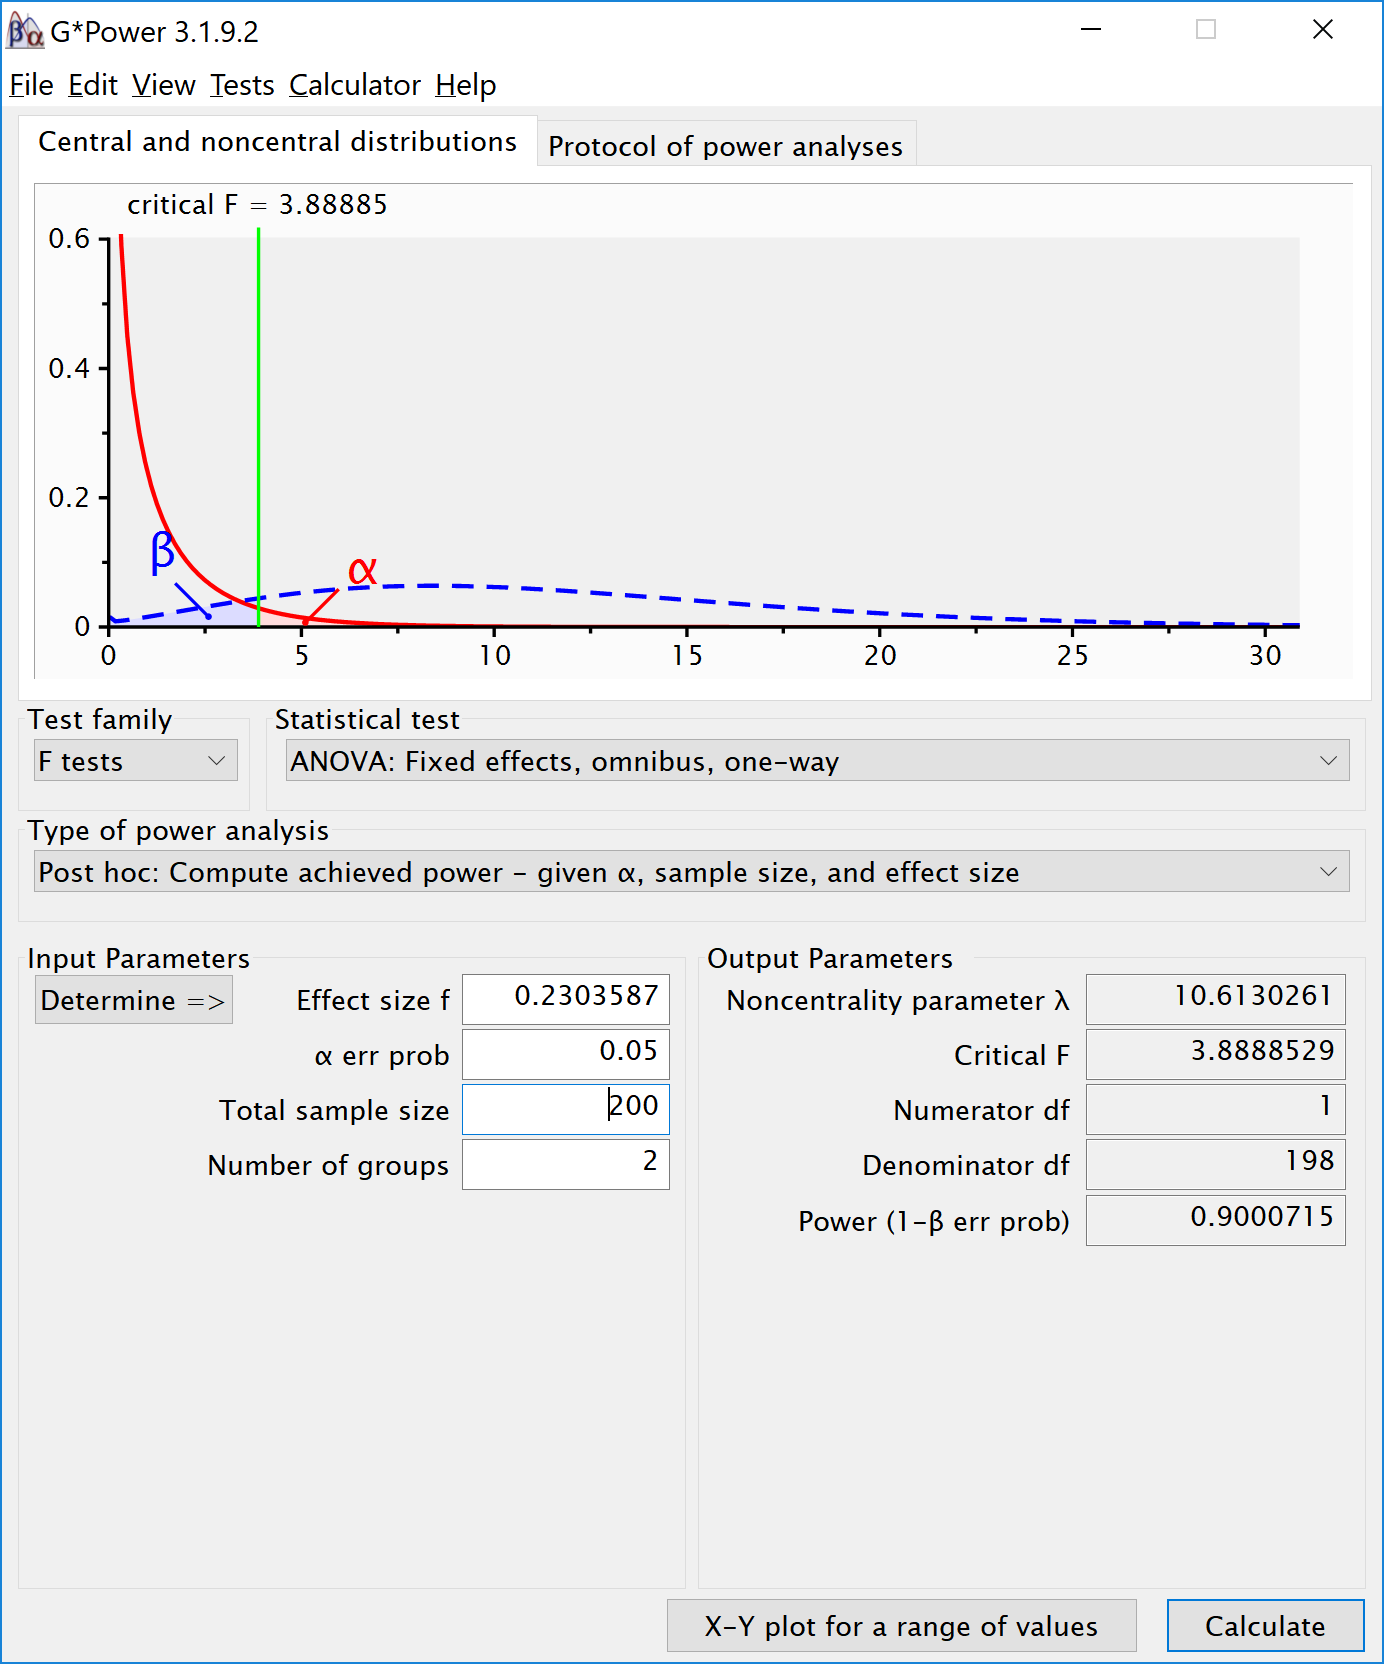
\includegraphics{screenshots/gpower_8.png}

A three-way ANOVA builds on the same principles as a one-way ANOVA. We look at whether the differences between groups are large, compared to the standard deviation. For the main effects we simply have 2 groups of 200 participants, and 2 means. If the population standard deviations are identical across groups, this is not in any way different from a one-way ANOVA. Indeed, we can show this by simulating a one-way ANOVA, where instead of 8 conditions, we have two conditions, and we average over the 4 groups of the other two factors. For example, for the main effect of size above can be computed analytically. There might be a small difference in the degrees of freedom of the two tests, or it is just random variation (And it will disappear when the number of iterations in the simulation, \texttt{nsim}, is increased).

\begin{Shaded}
\begin{Highlighting}[]
\NormalTok{string <-}\StringTok{ "2b"}
\NormalTok{n <-}\StringTok{ }\DecValTok{200}
\NormalTok{mu <-}\StringTok{ }\KeywordTok{c}\NormalTok{(}\KeywordTok{mean}\NormalTok{(}\KeywordTok{c}\NormalTok{(}\DecValTok{2}\NormalTok{, }\DecValTok{2}\NormalTok{, }\DecValTok{6}\NormalTok{, }\DecValTok{1}\NormalTok{)), }\KeywordTok{mean}\NormalTok{(}\KeywordTok{c}\NormalTok{(}\DecValTok{6}\NormalTok{, }\DecValTok{6}\NormalTok{, }\DecValTok{1}\NormalTok{, }\DecValTok{8}\NormalTok{)))}
\NormalTok{sd <-}\StringTok{ }\DecValTok{10}
\NormalTok{labelnames <-}\StringTok{ }\KeywordTok{c}\NormalTok{(}\StringTok{"Size"}\NormalTok{, }\StringTok{"big"}\NormalTok{, }\StringTok{"small"}\NormalTok{)}
\NormalTok{design_result <-}\StringTok{ }\KeywordTok{ANOVA_design}\NormalTok{(}\DataTypeTok{design =}\NormalTok{ string,}
                   \DataTypeTok{n =}\NormalTok{ n, }
                   \DataTypeTok{mu =}\NormalTok{ mu, }
                   \DataTypeTok{sd =}\NormalTok{ sd, }
                   \DataTypeTok{labelnames =}\NormalTok{ labelnames)}
\end{Highlighting}
\end{Shaded}

\begin{Shaded}
\begin{Highlighting}[]
\NormalTok{simulation_result <-}\StringTok{ }\KeywordTok{ANOVA_power}\NormalTok{(design_result, }
                                 \DataTypeTok{alpha_level =}\NormalTok{ alpha_level, }
                                 \DataTypeTok{nsims =}\NormalTok{ nsims,}
                                 \DataTypeTok{verbose =} \OtherTok{FALSE}\NormalTok{)}
\end{Highlighting}
\end{Shaded}

\begin{table}[!h]

\caption{\label{tab:unnamed-chunk-223}Simulated ANOVA Result}
\centering
\begin{tabular}{l|r|r}
\hline
  & power & effect\_size\\
\hline
anova\_Size & 70.69 & 0.0180045\\
\hline
\end{tabular}
\end{table}

\begin{Shaded}
\begin{Highlighting}[]
\NormalTok{exact_result <-}\StringTok{ }\KeywordTok{ANOVA_exact}\NormalTok{(design_result,}
                            \DataTypeTok{alpha_level =}\NormalTok{ alpha_level,}
                            \DataTypeTok{verbose =} \OtherTok{FALSE}\NormalTok{)}
\end{Highlighting}
\end{Shaded}

\begin{table}[!h]

\caption{\label{tab:unnamed-chunk-225}Exact ANOVA Result}
\centering
\begin{tabular}{l|r|r|r|r}
\hline
  & power & partial\_eta\_squared & cohen\_f & non\_centrality\\
\hline
Size & 70.33333 & 0.0154607 & 0.1253137 & 6.25\\
\hline
\end{tabular}
\end{table}

\begin{Shaded}
\begin{Highlighting}[]
\CommentTok{# Power based on analytical solution}
\KeywordTok{power_oneway_between}\NormalTok{(design_result)}\OperatorTok{$}\NormalTok{power }
\end{Highlighting}
\end{Shaded}

\begin{verbatim}
## [1] 70.33333
\end{verbatim}

Similarly, we can create a 2 factor design where we average over the third factor, and recreate the power analysis for the Two-Way interaction. For example, we can group over the Cognitive Load condition, and look at the Size by Color Interaction:

\begin{Shaded}
\begin{Highlighting}[]
\NormalTok{string <-}\StringTok{ "2b*2b"}
\NormalTok{n <-}\StringTok{ }\DecValTok{100}
\NormalTok{mu <-}\StringTok{ }\KeywordTok{c}\NormalTok{(}\KeywordTok{mean}\NormalTok{(}\KeywordTok{c}\NormalTok{(}\DecValTok{1}\NormalTok{, }\DecValTok{1}\NormalTok{)), }\KeywordTok{mean}\NormalTok{(}\KeywordTok{c}\NormalTok{(}\DecValTok{6}\NormalTok{, }\DecValTok{1}\NormalTok{)), }\KeywordTok{mean}\NormalTok{(}\KeywordTok{c}\NormalTok{(}\DecValTok{6}\NormalTok{, }\DecValTok{6}\NormalTok{)), }\KeywordTok{mean}\NormalTok{(}\KeywordTok{c}\NormalTok{(}\DecValTok{1}\NormalTok{, }\DecValTok{6}\NormalTok{)))}
\NormalTok{sd <-}\StringTok{ }\DecValTok{10}
\NormalTok{labelnames <-}\StringTok{ }\KeywordTok{c}\NormalTok{(}\StringTok{"Size"}\NormalTok{, }\StringTok{"big"}\NormalTok{, }\StringTok{"small"}\NormalTok{, }\StringTok{"Color"}\NormalTok{, }\StringTok{"green"}\NormalTok{, }\StringTok{"red"}\NormalTok{)}
\NormalTok{design_result <-}\StringTok{ }\KeywordTok{ANOVA_design}\NormalTok{(}\DataTypeTok{design =}\NormalTok{ string,}
                   \DataTypeTok{n =}\NormalTok{ n, }
                   \DataTypeTok{mu =}\NormalTok{ mu, }
                   \DataTypeTok{sd =}\NormalTok{ sd, }
                   \DataTypeTok{labelnames =}\NormalTok{ labelnames)}
\end{Highlighting}
\end{Shaded}

\begin{Shaded}
\begin{Highlighting}[]
\NormalTok{simulation_result <-}\StringTok{ }\KeywordTok{ANOVA_power}\NormalTok{(design_result, }
                                 \DataTypeTok{alpha_level =}\NormalTok{ alpha_level, }
                                 \DataTypeTok{nsims =}\NormalTok{ nsims,}
                                 \DataTypeTok{verbose =} \OtherTok{FALSE}\NormalTok{)}
\end{Highlighting}
\end{Shaded}

\begin{table}[!h]

\caption{\label{tab:unnamed-chunk-229}Simulated ANOVA Result}
\centering
\begin{tabular}{l|r|r}
\hline
  & power & effect\_size\\
\hline
anova\_Size & 70.93 & 0.0178407\\
\hline
anova\_Color & 5.20 & 0.0025269\\
\hline
anova\_Size:Color & 69.72 & 0.0176374\\
\hline
\end{tabular}
\end{table}

\begin{Shaded}
\begin{Highlighting}[]
\NormalTok{exact_result <-}\StringTok{ }\KeywordTok{ANOVA_exact}\NormalTok{(design_result,}
                            \DataTypeTok{alpha_level =}\NormalTok{ alpha_level,}
                            \DataTypeTok{verbose =} \OtherTok{FALSE}\NormalTok{)}
\end{Highlighting}
\end{Shaded}

\begin{table}[!h]

\caption{\label{tab:unnamed-chunk-231}Exact ANOVA Result}
\centering
\begin{tabular}{l|r|r|r|r}
\hline
  & power & partial\_eta\_squared & cohen\_f & non\_centrality\\
\hline
Size & 70.33227 & 0.0155376 & 0.1256297 & 6.25\\
\hline
Color & 5.00000 & 0.0000000 & 0.0000000 & 0.00\\
\hline
Size:Color & 70.33227 & 0.0155376 & 0.1256297 & 6.25\\
\hline
\end{tabular}
\end{table}

\begin{Shaded}
\begin{Highlighting}[]
\CommentTok{# Power based on analytical solution}
\NormalTok{power_res <-}\StringTok{ }\KeywordTok{power_twoway_between}\NormalTok{(design_result) }
\NormalTok{power_res}\OperatorTok{$}\NormalTok{power_A}
\end{Highlighting}
\end{Shaded}

\begin{verbatim}
## [1] 70.33228
\end{verbatim}

\begin{Shaded}
\begin{Highlighting}[]
\NormalTok{power_res}\OperatorTok{$}\NormalTok{power_B}
\end{Highlighting}
\end{Shaded}

\begin{verbatim}
## [1] 5
\end{verbatim}

\begin{Shaded}
\begin{Highlighting}[]
\NormalTok{power_res}\OperatorTok{$}\NormalTok{power_AB}
\end{Highlighting}
\end{Shaded}

\begin{verbatim}
## [1] 70.33228
\end{verbatim}

\begin{Shaded}
\begin{Highlighting}[]
\NormalTok{string <-}\StringTok{ "2b*2b*2b"}
\NormalTok{n <-}\StringTok{ }\DecValTok{50}
\NormalTok{mu <-}\StringTok{ }\KeywordTok{c}\NormalTok{(}\DecValTok{5}\NormalTok{, }\DecValTok{3}\NormalTok{, }\DecValTok{2}\NormalTok{, }\DecValTok{6}\NormalTok{, }\DecValTok{1}\NormalTok{, }\DecValTok{4}\NormalTok{, }\DecValTok{3}\NormalTok{, }\DecValTok{1}\NormalTok{) }
\NormalTok{sd <-}\StringTok{ }\DecValTok{10}
\NormalTok{r <-}\StringTok{ }\FloatTok{0.0}
\NormalTok{labelnames <-}\StringTok{ }\KeywordTok{c}\NormalTok{(}\StringTok{"Size"}\NormalTok{, }\StringTok{"big"}\NormalTok{, }\StringTok{"small"}\NormalTok{, }
                \StringTok{"Color"}\NormalTok{, }\StringTok{"green"}\NormalTok{, }\StringTok{"red"}\NormalTok{, }
                \StringTok{"CognitiveLoad"}\NormalTok{, }\StringTok{"present"}\NormalTok{, }\StringTok{"absent"}\NormalTok{) }
\NormalTok{design_result <-}\StringTok{ }\KeywordTok{ANOVA_design}\NormalTok{(}\DataTypeTok{design =}\NormalTok{ string,}
                   \DataTypeTok{n =}\NormalTok{ n, }
                   \DataTypeTok{mu =}\NormalTok{ mu, }
                   \DataTypeTok{sd =}\NormalTok{ sd, }
                   \DataTypeTok{labelnames =}\NormalTok{ labelnames)}
\end{Highlighting}
\end{Shaded}

\begin{Shaded}
\begin{Highlighting}[]
\NormalTok{simulation_result <-}\StringTok{ }\KeywordTok{ANOVA_power}\NormalTok{(design_result, }
                                 \DataTypeTok{alpha_level =}\NormalTok{ alpha_level, }
                                 \DataTypeTok{nsims =}\NormalTok{ nsims,}
                                 \DataTypeTok{verbose =} \OtherTok{FALSE}\NormalTok{)}
\end{Highlighting}
\end{Shaded}

\begin{table}[!h]

\caption{\label{tab:unnamed-chunk-235}Simulated ANOVA Result}
\centering
\begin{tabular}{l|r|r}
\hline
  & power & effect\_size\\
\hline
anova\_Size & 42.71 & 0.0103728\\
\hline
anova\_Color & 5.52 & 0.0026837\\
\hline
anova\_CognitiveLoad & 11.10 & 0.0038783\\
\hline
anova\_Size:Color & 5.74 & 0.0026956\\
\hline
anova\_Size:CognitiveLoad & 6.05 & 0.0027663\\
\hline
anova\_Color:CognitiveLoad & 5.69 & 0.0027028\\
\hline
anova\_Size:Color:CognitiveLoad & 78.13 & 0.0213083\\
\hline
\end{tabular}
\end{table}

\begin{Shaded}
\begin{Highlighting}[]
\NormalTok{exact_result <-}\StringTok{ }\KeywordTok{ANOVA_exact}\NormalTok{(design_result,}
                            \DataTypeTok{alpha_level =}\NormalTok{ alpha_level,}
                            \DataTypeTok{verbose =} \OtherTok{FALSE}\NormalTok{)}
\end{Highlighting}
\end{Shaded}

\begin{table}[!h]

\caption{\label{tab:unnamed-chunk-237}Exact ANOVA Result}
\centering
\begin{tabular}{l|r|r|r|r}
\hline
  & power & partial\_eta\_squared & cohen\_f & non\_centrality\\
\hline
Size & 41.52809 & 0.0077519 & 0.0883883 & 3.0625\\
\hline
Color & 5.71548 & 0.0001594 & 0.0126269 & 0.0625\\
\hline
CognitiveLoad & 11.61777 & 0.0014329 & 0.0378807 & 0.5625\\
\hline
Size:Color & 5.71548 & 0.0001594 & 0.0126269 & 0.0625\\
\hline
Size:CognitiveLoad & 5.71548 & 0.0001594 & 0.0126269 & 0.0625\\
\hline
Color:CognitiveLoad & 5.71548 & 0.0001594 & 0.0126269 & 0.0625\\
\hline
Size:Color:CognitiveLoad & 78.32737 & 0.0189270 & 0.1388960 & 7.5625\\
\hline
\end{tabular}
\end{table}

\begin{Shaded}
\begin{Highlighting}[]
\CommentTok{#Analytical power calculation}
\NormalTok{power_analytic <-}\StringTok{ }\KeywordTok{power_threeway_between}\NormalTok{(design_result)}
\NormalTok{power_analytic}\OperatorTok{$}\NormalTok{power_A}
\end{Highlighting}
\end{Shaded}

\begin{verbatim}
## [1] 41.5306
\end{verbatim}

\begin{Shaded}
\begin{Highlighting}[]
\NormalTok{power_analytic}\OperatorTok{$}\NormalTok{power_B}
\end{Highlighting}
\end{Shaded}

\begin{verbatim}
## [1] 5.715533
\end{verbatim}

\begin{Shaded}
\begin{Highlighting}[]
\NormalTok{power_analytic}\OperatorTok{$}\NormalTok{power_C}
\end{Highlighting}
\end{Shaded}

\begin{verbatim}
## [1] 11.61827
\end{verbatim}

\begin{Shaded}
\begin{Highlighting}[]
\NormalTok{power_analytic}\OperatorTok{$}\NormalTok{power_AB}
\end{Highlighting}
\end{Shaded}

\begin{verbatim}
## [1] 5.715533
\end{verbatim}

\begin{Shaded}
\begin{Highlighting}[]
\NormalTok{power_analytic}\OperatorTok{$}\NormalTok{power_AC}
\end{Highlighting}
\end{Shaded}

\begin{verbatim}
## [1] 5.715533
\end{verbatim}

\begin{Shaded}
\begin{Highlighting}[]
\NormalTok{power_analytic}\OperatorTok{$}\NormalTok{power_BC}
\end{Highlighting}
\end{Shaded}

\begin{verbatim}
## [1] 5.715533
\end{verbatim}

\begin{Shaded}
\begin{Highlighting}[]
\NormalTok{power_analytic}\OperatorTok{$}\NormalTok{power_ABC}
\end{Highlighting}
\end{Shaded}

\begin{verbatim}
## [1] 78.33036
\end{verbatim}

\begin{Shaded}
\begin{Highlighting}[]
\NormalTok{power_analytic}\OperatorTok{$}\NormalTok{eta_p_}\DecValTok{2}\NormalTok{_A}
\end{Highlighting}
\end{Shaded}

\begin{verbatim}
## [1] 0.007598077
\end{verbatim}

\begin{Shaded}
\begin{Highlighting}[]
\NormalTok{power_analytic}\OperatorTok{$}\NormalTok{eta_p_}\DecValTok{2}\NormalTok{_B}
\end{Highlighting}
\end{Shaded}

\begin{verbatim}
## [1] 0.0001562256
\end{verbatim}

\begin{Shaded}
\begin{Highlighting}[]
\NormalTok{power_analytic}\OperatorTok{$}\NormalTok{eta_p_}\DecValTok{2}\NormalTok{_C}
\end{Highlighting}
\end{Shaded}

\begin{verbatim}
## [1] 0.001404275
\end{verbatim}

\begin{Shaded}
\begin{Highlighting}[]
\NormalTok{power_analytic}\OperatorTok{$}\NormalTok{eta_p_}\DecValTok{2}\NormalTok{_AB}
\end{Highlighting}
\end{Shaded}

\begin{verbatim}
## [1] 0.0001562256
\end{verbatim}

\begin{Shaded}
\begin{Highlighting}[]
\NormalTok{power_analytic}\OperatorTok{$}\NormalTok{eta_p_}\DecValTok{2}\NormalTok{_AC}
\end{Highlighting}
\end{Shaded}

\begin{verbatim}
## [1] 0.0001562256
\end{verbatim}

\begin{Shaded}
\begin{Highlighting}[]
\NormalTok{power_analytic}\OperatorTok{$}\NormalTok{eta_p_}\DecValTok{2}\NormalTok{_BC}
\end{Highlighting}
\end{Shaded}

\begin{verbatim}
## [1] 0.0001562256
\end{verbatim}

\begin{Shaded}
\begin{Highlighting}[]
\NormalTok{power_analytic}\OperatorTok{$}\NormalTok{eta_p_}\DecValTok{2}\NormalTok{_ABC}
\end{Highlighting}
\end{Shaded}

\begin{verbatim}
## [1] 0.01855544
\end{verbatim}

The power for interactions depends on Cohen's \emph{f}, the alpha level, the sample size, and the degrees of freedom.

\begin{Shaded}
\begin{Highlighting}[]
\CommentTok{# With 2x2x2 designs, }
\CommentTok{# the names for paired comparisons can become very long. }
\CommentTok{# So here the sample size abbreviate terms}
\CommentTok{# Size, Color, and Cognitive Load, have values:}
\CommentTok{# b = big, s = small, g = green, }
\CommentTok{# r = red, pres = present, abs = absent.  }
\NormalTok{labelnames <-}\StringTok{ }\KeywordTok{c}\NormalTok{(}\StringTok{"Size"}\NormalTok{, }\StringTok{"b"}\NormalTok{, }\StringTok{"s"}\NormalTok{, }\StringTok{"x"}\NormalTok{, }\StringTok{"Color"}\NormalTok{, }\StringTok{"g"}\NormalTok{, }\StringTok{"r"}\NormalTok{, }
                \StringTok{"Load"}\NormalTok{, }\StringTok{"pres"}\NormalTok{, }\StringTok{"abs"}\NormalTok{) }\CommentTok{#}
\NormalTok{design_result <-}\StringTok{ }\KeywordTok{ANOVA_design}\NormalTok{(}\DataTypeTok{design =} \StringTok{"3b*2b*2b"}\NormalTok{, }
                              \DataTypeTok{n =} \DecValTok{15}\NormalTok{, }
                              \DataTypeTok{mu =} \KeywordTok{c}\NormalTok{(}\DecValTok{20}\NormalTok{, }\DecValTok{0}\NormalTok{, }\DecValTok{0}\NormalTok{, }\DecValTok{0}\NormalTok{, }\DecValTok{0}\NormalTok{, }
                                     \DecValTok{0}\NormalTok{, }\DecValTok{0}\NormalTok{, }\DecValTok{0}\NormalTok{, }\DecValTok{0}\NormalTok{, }\DecValTok{0}\NormalTok{, }\DecValTok{0}\NormalTok{, }\DecValTok{20}\NormalTok{), }
                              
                              \DataTypeTok{sd =} \DecValTok{20}\NormalTok{, }
                              \DataTypeTok{labelnames =}\NormalTok{ labelnames) }

\CommentTok{# Power based on exact simulations}
\NormalTok{exact_result <-}\StringTok{ }\KeywordTok{ANOVA_exact}\NormalTok{(design_result,}
                            \DataTypeTok{verbose =} \OtherTok{FALSE}\NormalTok{)}
\end{Highlighting}
\end{Shaded}

\begin{table}[!h]

\caption{\label{tab:unnamed-chunk-240}Exact ANOVA Result}
\centering
\begin{tabular}{l|r|r|r|r}
\hline
  & power & partial\_eta\_squared & cohen\_f & non\_centrality\\
\hline
Size & 26.92604 & 0.0146628 & 0.1219875 & 2.5\\
\hline
Color & 5.00000 & 0.0000000 & 0.0000000 & 0.0\\
\hline
Load & 5.00000 & 0.0000000 & 0.0000000 & 0.0\\
\hline
Size:Color & 67.93217 & 0.0427350 & 0.2112886 & 7.5\\
\hline
Size:Load & 67.93217 & 0.0427350 & 0.2112886 & 7.5\\
\hline
Color:Load & 60.38579 & 0.0289017 & 0.1725164 & 5.0\\
\hline
Size:Color:Load & 26.92604 & 0.0146628 & 0.1219875 & 2.5\\
\hline
\end{tabular}
\end{table}

\begin{Shaded}
\begin{Highlighting}[]
\CommentTok{#Analytical power calculation}
\NormalTok{power_analytic <-}\StringTok{ }\KeywordTok{power_threeway_between}\NormalTok{(design_result)}
\end{Highlighting}
\end{Shaded}

\begin{verbatim}
## Warning in sqrt(f_2_ABC): NaNs produced
\end{verbatim}

\begin{verbatim}
## Warning in pf(F_critical_ABC, df_ABC, df_error, lambda_ABC, lower.tail =
## FALSE): NaNs produced
\end{verbatim}

\begin{Shaded}
\begin{Highlighting}[]
\NormalTok{power_analytic}\OperatorTok{$}\NormalTok{power_A}
\end{Highlighting}
\end{Shaded}

\begin{verbatim}
## [1] 5
\end{verbatim}

\begin{Shaded}
\begin{Highlighting}[]
\NormalTok{power_analytic}\OperatorTok{$}\NormalTok{power_B}
\end{Highlighting}
\end{Shaded}

\begin{verbatim}
## [1] 5
\end{verbatim}

\begin{Shaded}
\begin{Highlighting}[]
\NormalTok{power_analytic}\OperatorTok{$}\NormalTok{power_C}
\end{Highlighting}
\end{Shaded}

\begin{verbatim}
## [1] 48.6496
\end{verbatim}

\begin{Shaded}
\begin{Highlighting}[]
\NormalTok{power_analytic}\OperatorTok{$}\NormalTok{power_AB}
\end{Highlighting}
\end{Shaded}

\begin{verbatim}
## [1] 34.7961
\end{verbatim}

\begin{Shaded}
\begin{Highlighting}[]
\NormalTok{power_analytic}\OperatorTok{$}\NormalTok{power_AC}
\end{Highlighting}
\end{Shaded}

\begin{verbatim}
## [1] 67.97466
\end{verbatim}

\begin{Shaded}
\begin{Highlighting}[]
\NormalTok{power_analytic}\OperatorTok{$}\NormalTok{power_BC}
\end{Highlighting}
\end{Shaded}

\begin{verbatim}
## [1] 91.55713
\end{verbatim}

\begin{Shaded}
\begin{Highlighting}[]
\NormalTok{power_analytic}\OperatorTok{$}\NormalTok{power_ABC}
\end{Highlighting}
\end{Shaded}

\begin{verbatim}
## [1] NaN
\end{verbatim}

\begin{Shaded}
\begin{Highlighting}[]
\NormalTok{power_analytic}\OperatorTok{$}\NormalTok{eta_p_}\DecValTok{2}\NormalTok{_A}
\end{Highlighting}
\end{Shaded}

\begin{verbatim}
## [1] 0
\end{verbatim}

\begin{Shaded}
\begin{Highlighting}[]
\NormalTok{power_analytic}\OperatorTok{$}\NormalTok{Cohen_f_A}
\end{Highlighting}
\end{Shaded}

\begin{verbatim}
## [1] 0
\end{verbatim}

We see that a pattern of means of 0, 0, 0, 0, 0, 0, 0, 20 for a 2x2x2 interaction equals a Cohen's \emph{f} of 0.25.

\begin{Shaded}
\begin{Highlighting}[]
\NormalTok{labelnames <-}\StringTok{ }\KeywordTok{c}\NormalTok{(}\StringTok{"Size"}\NormalTok{, }\StringTok{"b"}\NormalTok{, }\StringTok{"s"}\NormalTok{, }\StringTok{"Color"}\NormalTok{, }\StringTok{"g"}\NormalTok{, }\StringTok{"r"}\NormalTok{)}
\NormalTok{design_result <-}\StringTok{ }\KeywordTok{ANOVA_design}\NormalTok{(}\DataTypeTok{design =} \StringTok{"2b*2b"}\NormalTok{, }
                              \DataTypeTok{n =} \DecValTok{10}\NormalTok{, }
                              \DataTypeTok{mu =} \KeywordTok{c}\NormalTok{(}\DecValTok{0}\NormalTok{, }\DecValTok{0}\NormalTok{, }\DecValTok{0}\NormalTok{, }\DecValTok{10}\NormalTok{), }
                              \DataTypeTok{sd =} \DecValTok{10}\NormalTok{, }
                              \DataTypeTok{labelnames =}\NormalTok{ labelnames) }

\CommentTok{# Power based on exact simulations}
\NormalTok{exact_result <-}\StringTok{ }\KeywordTok{ANOVA_exact}\NormalTok{(design_result,}
                            \DataTypeTok{verbose =} \OtherTok{FALSE}\NormalTok{)}
\end{Highlighting}
\end{Shaded}

\begin{table}[!h]

\caption{\label{tab:unnamed-chunk-243}Exact ANOVA Result}
\centering
\begin{tabular}{l|r|r|r|r}
\hline
  & power & partial\_eta\_squared & cohen\_f & non\_centrality\\
\hline
Size & 33.71329 & 0.0649351 & 0.2635231 & 2.5\\
\hline
Color & 33.71329 & 0.0649351 & 0.2635231 & 2.5\\
\hline
Size:Color & 33.71329 & 0.0649351 & 0.2635231 & 2.5\\
\hline
\end{tabular}
\end{table}

\begin{Shaded}
\begin{Highlighting}[]
\CommentTok{#Analytical power calculation}
\NormalTok{power_analytic <-}\StringTok{ }\KeywordTok{power_twoway_between}\NormalTok{(design_result)}
\NormalTok{power_analytic}\OperatorTok{$}\NormalTok{power_A}
\end{Highlighting}
\end{Shaded}

\begin{verbatim}
## [1] 33.71329
\end{verbatim}

\begin{Shaded}
\begin{Highlighting}[]
\NormalTok{power_analytic}\OperatorTok{$}\NormalTok{eta_p_}\DecValTok{2}\NormalTok{_A}
\end{Highlighting}
\end{Shaded}

\begin{verbatim}
## [1] 0.05882353
\end{verbatim}

\begin{Shaded}
\begin{Highlighting}[]
\NormalTok{power_analytic}\OperatorTok{$}\NormalTok{Cohen_f_A}
\end{Highlighting}
\end{Shaded}

\begin{verbatim}
## [1] 0.25
\end{verbatim}

Cohen's \emph{f} is twice as large for a 2x2 design with the same mean value in one of four cells. In a 2 factor between design.

\begin{Shaded}
\begin{Highlighting}[]
\NormalTok{labelnames <-}\StringTok{ }\KeywordTok{c}\NormalTok{(}\StringTok{"Size"}\NormalTok{, }\StringTok{"b"}\NormalTok{, }\StringTok{"s"}\NormalTok{)}
\NormalTok{design_result <-}\StringTok{ }\KeywordTok{ANOVA_design}\NormalTok{(}\DataTypeTok{design =} \StringTok{"2b"}\NormalTok{, }
                              \DataTypeTok{n =} \DecValTok{10}\NormalTok{,  }
                              \DataTypeTok{mu =} \KeywordTok{c}\NormalTok{(}\DecValTok{0}\NormalTok{, }\DecValTok{5}\NormalTok{), }
                              \DataTypeTok{sd =} \DecValTok{10}\NormalTok{, }
                              \DataTypeTok{labelnames =}\NormalTok{ labelnames) }

\CommentTok{# Power based on exact simulations}
\NormalTok{exact_result <-}\StringTok{ }\KeywordTok{ANOVA_exact}\NormalTok{(design_result,}
                            \DataTypeTok{verbose =} \OtherTok{FALSE}\NormalTok{)}
\end{Highlighting}
\end{Shaded}

\begin{table}[!h]

\caption{\label{tab:unnamed-chunk-246}Exact ANOVA Result}
\centering
\begin{tabular}{l|r|r|r|r}
\hline
  & power & partial\_eta\_squared & cohen\_f & non\_centrality\\
\hline
Size & 18.50957 & 0.0649351 & 0.2635231 & 1.25\\
\hline
\end{tabular}
\end{table}

\begin{Shaded}
\begin{Highlighting}[]
\CommentTok{#Analytical power calculation}
\NormalTok{power_analytic <-}\StringTok{ }\KeywordTok{power_oneway_between}\NormalTok{(design_result)}
\NormalTok{power_analytic}\OperatorTok{$}\NormalTok{power}
\end{Highlighting}
\end{Shaded}

\begin{verbatim}
## [1] 18.50957
\end{verbatim}

\begin{Shaded}
\begin{Highlighting}[]
\NormalTok{power_analytic}\OperatorTok{$}\NormalTok{eta_p_}\DecValTok{2}
\end{Highlighting}
\end{Shaded}

\begin{verbatim}
## [1] 0.05882353
\end{verbatim}

\begin{Shaded}
\begin{Highlighting}[]
\NormalTok{power_analytic}\OperatorTok{$}\NormalTok{Cohen_f}
\end{Highlighting}
\end{Shaded}

\begin{verbatim}
## [1] 0.25
\end{verbatim}

\hypertarget{the-no-way-interactions}{%
\chapter{The `No-Way' Interactions}\label{the-no-way-interactions}}

In the 17th Data Colada blog post titled \href{http://datacolada.org/17}{No-way Interactions} \citet{simonsohn_2014} discusses how a moderated interaction (the effect is there in one condition, but disappears in another condition) requires at least twice as many subjects per cell as a study that simply aims to show the simple effect. For example, see the plot below. Assume the score on the vertical axis is desire for fruit, as a function of the fruit that is available (an apple or a banana) and how hungry people are (not, or very). We see there is a difference between the participants desire for a banana compared to an apple, but only for participants who are very hungry. The point that is made is that you need twice as many participants in each cell to have power for the interaction, as you need for the simple effect.

\begin{Shaded}
\begin{Highlighting}[]
\NormalTok{string <-}\StringTok{ "2b*2b"}
\NormalTok{n <-}\StringTok{ }\DecValTok{20}
\CommentTok{# All means are equal - so there is no real difference.}
\CommentTok{# Enter means in the order that matches the labels below.}
\NormalTok{mu <-}\StringTok{ }\KeywordTok{c}\NormalTok{(}\DecValTok{20}\NormalTok{, }\DecValTok{20}\NormalTok{, }\DecValTok{20}\NormalTok{, }\DecValTok{25}\NormalTok{) }
\NormalTok{sd <-}\StringTok{ }\FloatTok{0.5}
\NormalTok{labelnames <-}\StringTok{ }\KeywordTok{c}\NormalTok{(}\StringTok{"fruit"}\NormalTok{, }\StringTok{"apple"}\NormalTok{, }\StringTok{"banana"}\NormalTok{, }
                \StringTok{"hunger"}\NormalTok{, }\StringTok{"no hunger"}\NormalTok{, }\StringTok{"very hungry"}\NormalTok{) }\CommentTok{#}
\CommentTok{# the label names should be in the order of the means specified above.}
\NormalTok{design_result <-}\StringTok{ }\KeywordTok{ANOVA_design}\NormalTok{(}\DataTypeTok{design =}\NormalTok{ string,}
                   \DataTypeTok{n =}\NormalTok{ n, }
                   \DataTypeTok{mu =}\NormalTok{ mu, }
                   \DataTypeTok{sd =}\NormalTok{ sd, }
                   \DataTypeTok{labelnames =}\NormalTok{ labelnames,}
                   \DataTypeTok{plot =} \OtherTok{TRUE}\NormalTok{)}
\end{Highlighting}
\end{Shaded}

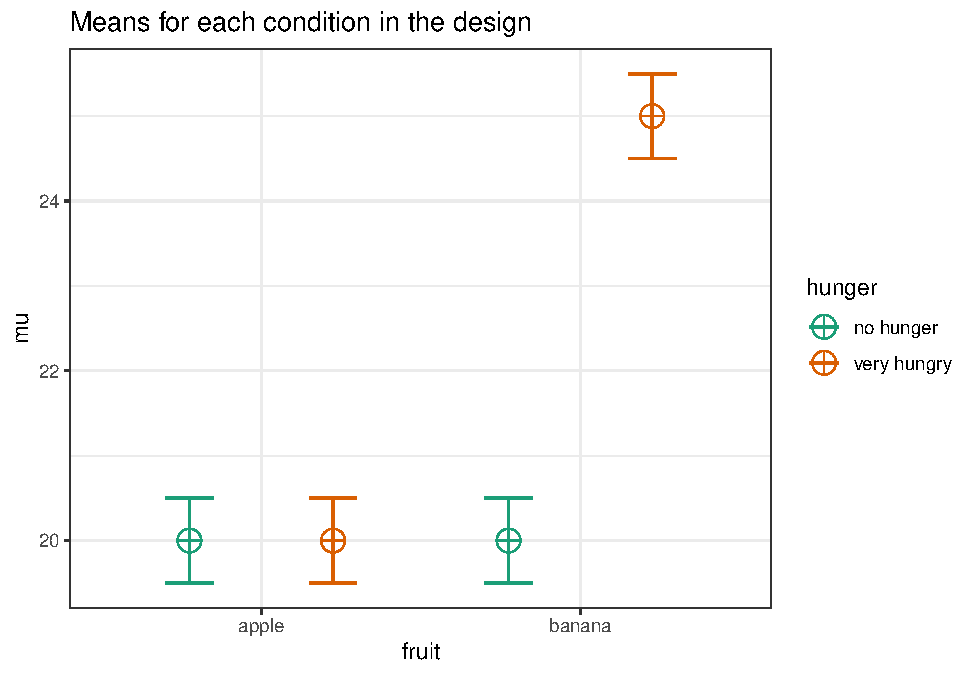
\includegraphics{SuperpowerValidation_files/figure-latex/unnamed-chunk-249-1.pdf}

We can reproduce the simulations in the Data Colada blog post, using the original code.

\begin{Shaded}
\begin{Highlighting}[]
\CommentTok{#R-Code}
\CommentTok{#}
\CommentTok{#Written by Uri Simonsohn, March 2014}
\CommentTok{#}
\CommentTok{#}
\CommentTok{#In DataColada[17] }
\CommentTok{# I propose that 2x2 interaction studies need 2x the sample size}
\CommentTok{#http://datacolada.org/2014/03/10/17-no-way-interactions}
\CommentTok{#In a companion ,pdf I show the simple math behind it}
\CommentTok{#}
\CommentTok{#}
\CommentTok{#Simulations are often more persuasive than math, so here it goes.}
\CommentTok{#I run simulations that compute power for 2 and 4 cell design, }
\CommentTok{# the latter testing the interaction}
\CommentTok{###############################################################################}
\CommentTok{#Create function that computes power of Studies 1 and 2, }
\CommentTok{# where Study 1  has 2 cells and tests a simple effect}
\CommentTok{#and Study 2 has 4 cells and tests the interaction}
\NormalTok{colada17 =}\StringTok{ }\ControlFlowTok{function}\NormalTok{(d1,d2,n1,n2,simtot)}
\NormalTok{  \{}
  \CommentTok{#n1: sample size, per cell, study 1}
  \CommentTok{#n2: sample size, per cell, study 2}
  \CommentTok{#d1: simple effect M1-M2}
  \CommentTok{#d2: moderated effect M3-M4, }
  \CommentTok{# full elimination of effect implies d2=0}
  \CommentTok{#simtot: how many simulations to run}
  \CommentTok{#Here we will store results}
\NormalTok{      p1 =}\StringTok{ }\KeywordTok{c}\NormalTok{()    }\CommentTok{#p-values for Study 1}
\NormalTok{      p2 =}\StringTok{ }\KeywordTok{c}\NormalTok{()    }\CommentTok{#p-values for Study 2}
  \ControlFlowTok{for}\NormalTok{ (i }\ControlFlowTok{in} \DecValTok{1}\OperatorTok{:}\NormalTok{simtot) \{}
    \CommentTok{#draw data 4 samples}
\NormalTok{    y1 =}\StringTok{ }\KeywordTok{rnorm}\NormalTok{(}\DataTypeTok{n =} \KeywordTok{max}\NormalTok{(n1, n2), }\DataTypeTok{mean =}\NormalTok{ d1)}
\NormalTok{    y2 =}\StringTok{ }\KeywordTok{rnorm}\NormalTok{(}\DataTypeTok{n =} \KeywordTok{max}\NormalTok{(n1, n2))}
\NormalTok{    y3 =}\StringTok{ }\KeywordTok{rnorm}\NormalTok{(}\DataTypeTok{n =} \KeywordTok{max}\NormalTok{(n1, n2), }\DataTypeTok{mean =}\NormalTok{ d2)}
\NormalTok{    y4 =}\StringTok{ }\KeywordTok{rnorm}\NormalTok{(}\DataTypeTok{n =} \KeywordTok{max}\NormalTok{(n1, n2))}
    
    \CommentTok{#GET DATA READY FOR ANOVA  }
\NormalTok{    y =}\StringTok{ }\KeywordTok{c}\NormalTok{(y1, y2, y3, y4)          }\CommentTok{#the d.v.}
\NormalTok{    nrep =}\StringTok{ }\KeywordTok{rep}\NormalTok{(n2, }\DecValTok{4}\NormalTok{)}
\NormalTok{    A =}\StringTok{ }\KeywordTok{rep}\NormalTok{(}\KeywordTok{c}\NormalTok{(}\DecValTok{1}\NormalTok{, }\DecValTok{1}\NormalTok{, }\DecValTok{0}\NormalTok{, }\DecValTok{0}\NormalTok{), }\DataTypeTok{times =}\NormalTok{ nrep)}
\NormalTok{    B =}\StringTok{ }\KeywordTok{rep}\NormalTok{(}\KeywordTok{c}\NormalTok{(}\DecValTok{1}\NormalTok{, }\DecValTok{0}\NormalTok{, }\DecValTok{1}\NormalTok{, }\DecValTok{0}\NormalTok{), }\DataTypeTok{times =}\NormalTok{ nrep)}
    
    \CommentTok{#STUDY 1}
      \CommentTok{#Do a t-test on the first n1 observations}
\NormalTok{      p1.k =}\StringTok{ }\KeywordTok{t.test}\NormalTok{(y1[}\DecValTok{1}\OperatorTok{:}\NormalTok{n1], y2[}\DecValTok{1}\OperatorTok{:}\NormalTok{n1], }\DataTypeTok{var.equal =} \OtherTok{TRUE}\NormalTok{)}\OperatorTok{$}\NormalTok{p.value  }
    
    \CommentTok{#STUDY 2}
      \CommentTok{#Do anova, keep p-value of the interaction}
\NormalTok{      p2.k =}\StringTok{ }\KeywordTok{anova}\NormalTok{(}\KeywordTok{lm}\NormalTok{(y }\OperatorTok{~}\StringTok{ }\NormalTok{A }\OperatorTok{*}\StringTok{ }\NormalTok{B))[}\StringTok{"A:B"}\NormalTok{, }\StringTok{"Pr(>F)"}\NormalTok{]             }
        
      \CommentTok{#Store the results}
\NormalTok{      p1 =}\StringTok{ }\KeywordTok{c}\NormalTok{(p1, p1.k)}
\NormalTok{      p2 =}\StringTok{ }\KeywordTok{c}\NormalTok{(p2, p2.k)}
    
\NormalTok{      \}}
  
  \CommentTok{#What share off comparisons are significant}
      \CommentTok{#Simple test using estimate of variance from 2 cells only}
\NormalTok{      power1 =}\StringTok{ }\KeywordTok{sum}\NormalTok{(p1 }\OperatorTok{<=}\StringTok{ }\FloatTok{.05}\NormalTok{) }\OperatorTok{/}\StringTok{ }\NormalTok{simtot  }
      \CommentTok{#Interaction}
\NormalTok{      power2 =}\StringTok{ }\KeywordTok{sum}\NormalTok{(p2 }\OperatorTok{<=}\StringTok{ }\FloatTok{.05}\NormalTok{) }\OperatorTok{/}\StringTok{ }\NormalTok{simtot  }
  
    \KeywordTok{cat}\NormalTok{(}\StringTok{"}\CharTok{\textbackslash{}n}\StringTok{Study 1 is powered to:"}\NormalTok{,}\KeywordTok{round}\NormalTok{(power1,}\DecValTok{2}\NormalTok{))}
    \KeywordTok{cat}\NormalTok{(}\StringTok{"}\CharTok{\textbackslash{}n}\StringTok{Study 2 is powered to:"}\NormalTok{,}\KeywordTok{round}\NormalTok{(power2,}\DecValTok{2}\NormalTok{))}
  
\NormalTok{    \}}
    
    
\CommentTok{#Same power for 2n regardless of n and d}
\end{Highlighting}
\end{Shaded}

\begin{Shaded}
\begin{Highlighting}[]
  \KeywordTok{colada17}\NormalTok{(}\DataTypeTok{simtot =} \DecValTok{2000}\NormalTok{, }\DataTypeTok{n1 =} \DecValTok{20}\NormalTok{, }\DataTypeTok{n2 =} \DecValTok{40}\NormalTok{, }\DataTypeTok{d1 =} \DecValTok{1}\NormalTok{, }\DataTypeTok{d2 =} \DecValTok{0}\NormalTok{)  }
\end{Highlighting}
\end{Shaded}

\begin{verbatim}
## 
## Study 1 is powered to: 0.85
\end{verbatim}

\begin{verbatim}
## 
## Study 2 is powered to: 0.89
\end{verbatim}

\begin{Shaded}
\begin{Highlighting}[]
  \KeywordTok{colada17}\NormalTok{(}\DataTypeTok{simtot =} \DecValTok{2000}\NormalTok{, }\DataTypeTok{n1 =} \DecValTok{50}\NormalTok{, }\DataTypeTok{n2 =} \DecValTok{100}\NormalTok{, }\DataTypeTok{d1 =} \FloatTok{.3}\NormalTok{, }\DataTypeTok{d2 =} \DecValTok{0}\NormalTok{)}
\end{Highlighting}
\end{Shaded}

\begin{verbatim}
## 
## Study 1 is powered to: 0.33
\end{verbatim}

\begin{verbatim}
## 
## Study 2 is powered to: 0.32
\end{verbatim}

\begin{Shaded}
\begin{Highlighting}[]
  \KeywordTok{colada17}\NormalTok{(}\DataTypeTok{simtot =} \DecValTok{2000}\NormalTok{, }\DataTypeTok{n1 =} \DecValTok{150}\NormalTok{, }\DataTypeTok{n2 =} \DecValTok{300}\NormalTok{, }\DataTypeTok{d1 =} \FloatTok{.25}\NormalTok{, }\DataTypeTok{d2 =} \DecValTok{0}\NormalTok{)}
\end{Highlighting}
\end{Shaded}

\begin{verbatim}
## 
## Study 1 is powered to: 0.56
\end{verbatim}

\begin{verbatim}
## 
## Study 2 is powered to: 0.58
\end{verbatim}

\begin{Shaded}
\begin{Highlighting}[]
\CommentTok{#Need 4n if effect is 70% attenuated}
  \KeywordTok{colada17}\NormalTok{(}\DataTypeTok{simtot =} \DecValTok{2000}\NormalTok{, }\DataTypeTok{n1 =} \DecValTok{25}\NormalTok{, }\DataTypeTok{n2 =} \DecValTok{100}\NormalTok{, }\DataTypeTok{d1 =} \FloatTok{.5}\NormalTok{, }\DataTypeTok{d2 =} \FloatTok{.3} \OperatorTok{*}\StringTok{ }\FloatTok{.5}\NormalTok{)}
\end{Highlighting}
\end{Shaded}

\begin{verbatim}
## 
## Study 1 is powered to: 0.4
\end{verbatim}

\begin{verbatim}
## 
## Study 2 is powered to: 0.4
\end{verbatim}

\begin{Shaded}
\begin{Highlighting}[]
  \KeywordTok{colada17}\NormalTok{(}\DataTypeTok{simtot =} \DecValTok{2000}\NormalTok{, }\DataTypeTok{n1 =} \DecValTok{50}\NormalTok{, }\DataTypeTok{n2 =} \DecValTok{200}\NormalTok{, }\DataTypeTok{d1 =} \FloatTok{.5}\NormalTok{, }\DataTypeTok{d2 =} \FloatTok{.3} \OperatorTok{*}\StringTok{ }\FloatTok{.5}\NormalTok{)}
\end{Highlighting}
\end{Shaded}

\begin{verbatim}
## 
## Study 1 is powered to: 0.71
\end{verbatim}

\begin{verbatim}
## 
## Study 2 is powered to: 0.68
\end{verbatim}

\begin{Shaded}
\begin{Highlighting}[]
  \KeywordTok{colada17}\NormalTok{(}\DataTypeTok{simtot =} \DecValTok{2000}\NormalTok{, }\DataTypeTok{n1 =} \DecValTok{22}\NormalTok{, }\DataTypeTok{n2 =} \DecValTok{88}\NormalTok{, }\DataTypeTok{d1 =} \FloatTok{.41}\NormalTok{, }\DataTypeTok{d2 =} \FloatTok{.3} \OperatorTok{*}\StringTok{ }\FloatTok{.41}\NormalTok{)}
\end{Highlighting}
\end{Shaded}

\begin{verbatim}
## 
## Study 1 is powered to: 0.28
\end{verbatim}

\begin{verbatim}
## 
## Study 2 is powered to: 0.25
\end{verbatim}

\begin{Shaded}
\begin{Highlighting}[]
\CommentTok{#underpowered if run with the same n}
\KeywordTok{colada17}\NormalTok{(}\DataTypeTok{simtot =}\NormalTok{ nsims, }\DataTypeTok{n1 =} \DecValTok{20}\NormalTok{, }\DataTypeTok{n2 =} \DecValTok{20}\NormalTok{, }\DataTypeTok{d1 =} \DecValTok{1}\NormalTok{, }\DataTypeTok{d2 =} \DecValTok{0}\NormalTok{)  }
\end{Highlighting}
\end{Shaded}

\begin{verbatim}
## 
## Study 1 is powered to: 0.87
\end{verbatim}

\begin{verbatim}
## 
## Study 2 is powered to: 0.59
\end{verbatim}

And we can reproduce the results using the \texttt{ANOVA\_exact} function.

\begin{Shaded}
\begin{Highlighting}[]
\CommentTok{#Study 1}
\NormalTok{string <-}\StringTok{ "2b*2b"}
\NormalTok{n <-}\StringTok{ }\DecValTok{10}
\CommentTok{# All means are equal - so there is no real difference.}
\CommentTok{# Enter means in the order that matches the labels below.}
\NormalTok{mu <-}\StringTok{ }\KeywordTok{c}\NormalTok{(}\DecValTok{1}\NormalTok{, }\DecValTok{2}\NormalTok{, }\DecValTok{1}\NormalTok{, }\DecValTok{2}\NormalTok{) }
\NormalTok{sd <-}\StringTok{ }\DecValTok{1}

\CommentTok{# the label names should be in the order of the means specified above.}
\NormalTok{design_result <-}\StringTok{ }\KeywordTok{ANOVA_design}\NormalTok{(}\DataTypeTok{design =}\NormalTok{ string,}
                   \DataTypeTok{n =}\NormalTok{ n, }
                   \DataTypeTok{mu =}\NormalTok{ mu, }
                   \DataTypeTok{sd =}\NormalTok{ sd, }
                   \DataTypeTok{plot =} \OtherTok{TRUE}\NormalTok{)}
\end{Highlighting}
\end{Shaded}

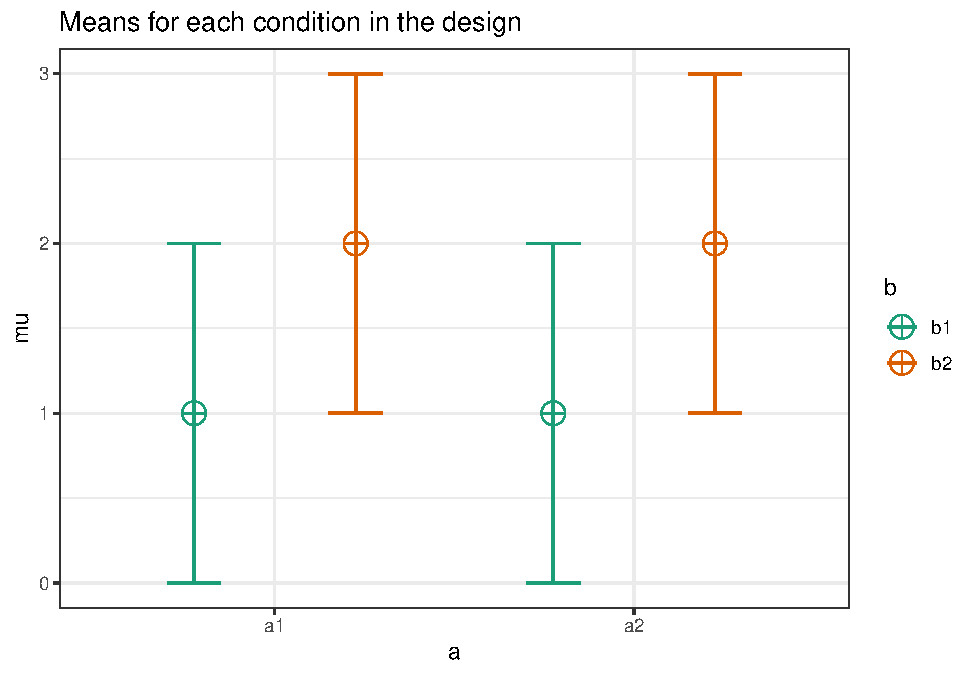
\includegraphics{SuperpowerValidation_files/figure-latex/unnamed-chunk-265-1.pdf}

\begin{Shaded}
\begin{Highlighting}[]
\NormalTok{alpha_level <-}\StringTok{ }\FloatTok{0.05} \CommentTok{#We set the alpha level at 0.05. }

\NormalTok{exact_result <-}\StringTok{ }\KeywordTok{ANOVA_exact}\NormalTok{(design_result, }
                            \DataTypeTok{alpha_level =}\NormalTok{ alpha_level,}
                            \DataTypeTok{verbose =} \OtherTok{FALSE}\NormalTok{)}

\NormalTok{knitr}\OperatorTok{::}\KeywordTok{kable}\NormalTok{(exact_result}\OperatorTok{$}\NormalTok{main_results[}\DecValTok{2}\NormalTok{,], }
             \DataTypeTok{caption =} \StringTok{"ANOVA Results"}\NormalTok{)}\OperatorTok
\StringTok{  }\KeywordTok{kable_styling}\NormalTok{(}\DataTypeTok{latex_options =} \StringTok{"hold_position"}\NormalTok{)}
\end{Highlighting}
\end{Shaded}

\begin{table}[!h]

\caption{\label{tab:unnamed-chunk-265}ANOVA Results}
\centering
\begin{tabular}{l|r|r|r|r}
\hline
  & power & partial\_eta\_squared & cohen\_f & non\_centrality\\
\hline
b & 86.79843 & 0.2173913 & 0.5270463 & 10\\
\hline
\end{tabular}
\end{table}

\begin{Shaded}
\begin{Highlighting}[]
\CommentTok{#Study 2}
\NormalTok{string <-}\StringTok{ "2b*2b"}
\NormalTok{n <-}\StringTok{ }\DecValTok{20}
\CommentTok{# All means are equal - so there is no real difference.}
\CommentTok{# Enter means in the order that matches the labels below.}
\NormalTok{mu <-}\StringTok{ }\KeywordTok{c}\NormalTok{(}\DecValTok{1}\NormalTok{, }\DecValTok{2}\NormalTok{, }\DecValTok{1}\NormalTok{, }\DecValTok{3}\NormalTok{) }
\NormalTok{sd <-}\StringTok{ }\DecValTok{1}

\CommentTok{# the label names should be in the order of the means specified above.}
\NormalTok{design_result <-}\StringTok{ }\KeywordTok{ANOVA_design}\NormalTok{(}\DataTypeTok{design =}\NormalTok{ string,}
                   \DataTypeTok{n =}\NormalTok{ n, }
                   \DataTypeTok{mu =}\NormalTok{ mu, }
                   \DataTypeTok{sd =}\NormalTok{ sd, }
                   \DataTypeTok{plot =} \OtherTok{TRUE}\NormalTok{)}
\end{Highlighting}
\end{Shaded}

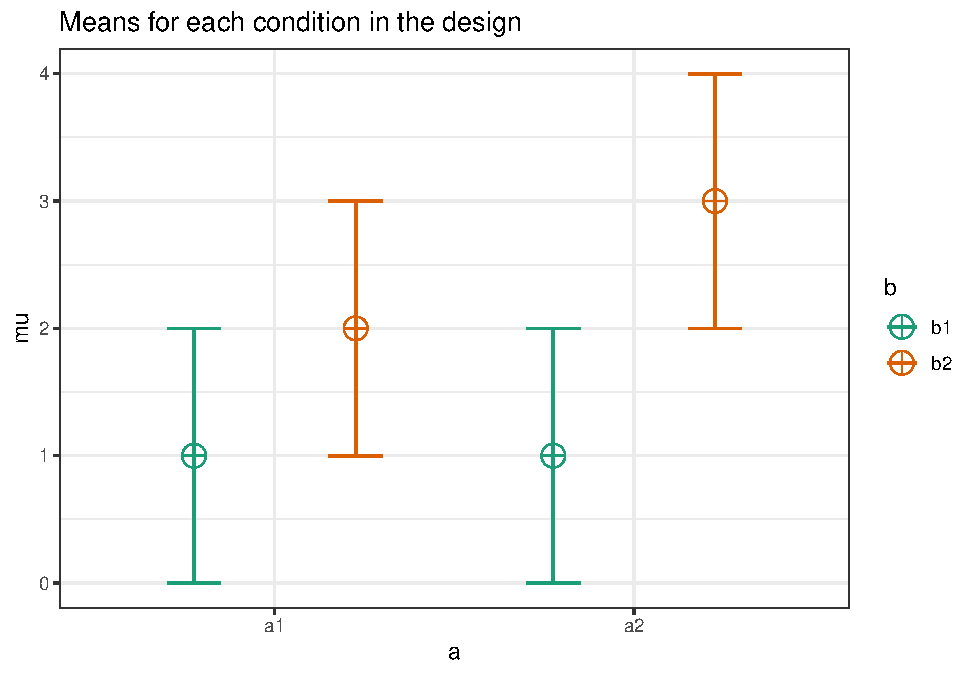
\includegraphics{SuperpowerValidation_files/figure-latex/unnamed-chunk-265-2.pdf}

\begin{Shaded}
\begin{Highlighting}[]
\NormalTok{alpha_level <-}\StringTok{ }\FloatTok{0.05} \CommentTok{#We set the alpha level at 0.05. }

\NormalTok{exact_result <-}\StringTok{ }\KeywordTok{ANOVA_exact}\NormalTok{(design_result, }
                            \DataTypeTok{alpha_level =}\NormalTok{ alpha_level,}
                            \DataTypeTok{verbose =} \OtherTok{FALSE}\NormalTok{)}

\NormalTok{knitr}\OperatorTok{::}\KeywordTok{kable}\NormalTok{(exact_result}\OperatorTok{$}\NormalTok{main_results[}\DecValTok{3}\NormalTok{,], }
             \DataTypeTok{caption =} \StringTok{"ANOVA Results"}\NormalTok{)}\OperatorTok
\StringTok{  }\KeywordTok{kable_styling}\NormalTok{(}\DataTypeTok{latex_options =} \StringTok{"hold_position"}\NormalTok{)}
\end{Highlighting}
\end{Shaded}

\begin{table}[!h]

\caption{\label{tab:unnamed-chunk-265}ANOVA Results}
\centering
\begin{tabular}{l|r|r|r|r}
\hline
  & power & partial\_eta\_squared & cohen\_f & non\_centrality\\
\hline
a:b & 59.78655 & 0.0617284 & 0.2564946 & 5\\
\hline
\end{tabular}
\end{table}

We see we get the same power for the anova\_fruit:hunger interaction and for the simple effect p\_fruit\_apple\_hunger\_very hungry\_fruit\_banana\_hunger\_very hungry as the simulations by Uri Simonsohn in his blog post.

\begin{Shaded}
\begin{Highlighting}[]
\CommentTok{#Same power for 2n regardless of n and d}
\KeywordTok{colada17}\NormalTok{(}\DataTypeTok{simtot =} \DecValTok{10000}\NormalTok{, }\DataTypeTok{n1 =} \DecValTok{20}\NormalTok{, }\DataTypeTok{n2 =} \DecValTok{40}\NormalTok{, }\DataTypeTok{d1 =} \DecValTok{1}\NormalTok{, }\DataTypeTok{d2 =} \DecValTok{0}\NormalTok{)  }

\KeywordTok{colada17}\NormalTok{(}\DataTypeTok{simtot =} \DecValTok{10000}\NormalTok{, }\DataTypeTok{n1 =} \DecValTok{20}\NormalTok{, }\DataTypeTok{n2 =} \DecValTok{40}\NormalTok{, }\DataTypeTok{d1 =} \DecValTok{1}\NormalTok{, }\DataTypeTok{d2 =} \DecValTok{0}\NormalTok{) }
\end{Highlighting}
\end{Shaded}

\begin{verbatim}
## 
## Study 1 is powered to: 0.87
\end{verbatim}

\begin{verbatim}
## 
## Study 2 is powered to: 0.88
\end{verbatim}

\begin{Shaded}
\begin{Highlighting}[]
\KeywordTok{colada17}\NormalTok{(}\DataTypeTok{simtot =} \DecValTok{10000}\NormalTok{, }\DataTypeTok{n1 =} \DecValTok{50}\NormalTok{, }\DataTypeTok{n2 =} \DecValTok{100}\NormalTok{, }\DataTypeTok{d1 =} \FloatTok{.3}\NormalTok{, }\DataTypeTok{d2 =} \DecValTok{0}\NormalTok{)}
\end{Highlighting}
\end{Shaded}

\begin{verbatim}
## 
## Study 1 is powered to: 0.32
\end{verbatim}

\begin{verbatim}
## 
## Study 2 is powered to: 0.33
\end{verbatim}

\begin{Shaded}
\begin{Highlighting}[]
\KeywordTok{colada17}\NormalTok{(}\DataTypeTok{simtot =} \DecValTok{10000}\NormalTok{, }\DataTypeTok{n1 =} \DecValTok{150}\NormalTok{, }\DataTypeTok{n2 =} \DecValTok{300}\NormalTok{, }\DataTypeTok{d1 =} \FloatTok{.25}\NormalTok{, }\DataTypeTok{d2 =} \DecValTok{0}\NormalTok{)}
\end{Highlighting}
\end{Shaded}

\begin{verbatim}
## 
## Study 1 is powered to: 0.58
\end{verbatim}

\begin{verbatim}
## 
## Study 2 is powered to: 0.58
\end{verbatim}

We can also reproduce the last example by adjusting the means and standard deviation. With 150 people, and a Cohen's d of 0.25 (the difference is 5, the sd 20, so 5/20 = 0.25) we should reproduce the power for the simple effect.

\begin{Shaded}
\begin{Highlighting}[]
\NormalTok{string <-}\StringTok{ "2b*2b"}
\NormalTok{n <-}\StringTok{ }\DecValTok{150}
\NormalTok{mu <-}\StringTok{ }\KeywordTok{c}\NormalTok{(}\DecValTok{20}\NormalTok{, }\DecValTok{20}\NormalTok{, }\DecValTok{20}\NormalTok{, }\DecValTok{25}\NormalTok{) }\CommentTok{#All means are equal - so there is no real difference.}
\CommentTok{# Enter means in the order that matches the labels below.}
\NormalTok{sd <-}\StringTok{ }\DecValTok{20}
\NormalTok{labelnames <-}\StringTok{ }\KeywordTok{c}\NormalTok{(}\StringTok{"fruit"}\NormalTok{, }\StringTok{"apple"}\NormalTok{, }\StringTok{"banana"}\NormalTok{, }
                \StringTok{"hunger"}\NormalTok{, }\StringTok{"no hunger"}\NormalTok{, }\StringTok{"very hungry"}\NormalTok{) }\CommentTok{#}
\CommentTok{# the label names should be in the order of the means specified above.}
\NormalTok{design_result <-}\StringTok{ }\KeywordTok{ANOVA_design}\NormalTok{(}\DataTypeTok{design =}\NormalTok{ string,}
                   \DataTypeTok{n =}\NormalTok{ n, }
                   \DataTypeTok{mu =}\NormalTok{ mu, }
                   \DataTypeTok{sd =}\NormalTok{ sd, }
                   \DataTypeTok{labelnames =}\NormalTok{ labelnames)}
\NormalTok{alpha_level <-}\StringTok{ }\FloatTok{0.05} \CommentTok{#We set the alpha level at 0.05. }

\NormalTok{exact_result <-}\StringTok{ }\KeywordTok{ANOVA_exact}\NormalTok{(design_result, }
                            \DataTypeTok{alpha_level =}\NormalTok{ alpha_level,}
                            \DataTypeTok{verbose =} \OtherTok{FALSE}\NormalTok{)}

\NormalTok{knitr}\OperatorTok{::}\KeywordTok{kable}\NormalTok{(exact_result}\OperatorTok{$}\NormalTok{main_results[}\DecValTok{2}\NormalTok{,], }
             \DataTypeTok{caption =} \StringTok{"ANOVA Results"}\NormalTok{)}\OperatorTok
\StringTok{  }\KeywordTok{kable_styling}\NormalTok{(}\DataTypeTok{latex_options =} \StringTok{"hold_position"}\NormalTok{)}
\end{Highlighting}
\end{Shaded}

\begin{table}[!h]

\caption{\label{tab:unnamed-chunk-272}ANOVA Results}
\centering
\begin{tabular}{l|r|r|r|r}
\hline
  & power & partial\_eta\_squared & cohen\_f & non\_centrality\\
\hline
hunger & 33.32955 & 0.0039171 & 0.0627094 & 2.34375\\
\hline
\end{tabular}
\end{table}

And changing the sample size to 300 should reproduce the power for the interaction in the ANOVA.

\begin{Shaded}
\begin{Highlighting}[]
\NormalTok{string <-}\StringTok{ "2b*2b"}
\NormalTok{n <-}\StringTok{ }\DecValTok{300}
\NormalTok{mu <-}\StringTok{ }\KeywordTok{c}\NormalTok{(}\DecValTok{20}\NormalTok{, }\DecValTok{20}\NormalTok{, }\DecValTok{20}\NormalTok{, }\DecValTok{25}\NormalTok{) }\CommentTok{#All means are equal - so there is no real difference.}
\CommentTok{# Enter means in the order that matches the labels below.}
\NormalTok{sd <-}\StringTok{ }\DecValTok{20}
\NormalTok{labelnames <-}\StringTok{ }\KeywordTok{c}\NormalTok{(}\StringTok{"fruit"}\NormalTok{, }\StringTok{"apple"}\NormalTok{, }\StringTok{"banana"}\NormalTok{, }
                \StringTok{"hunger"}\NormalTok{, }\StringTok{"no hunger"}\NormalTok{, }\StringTok{"very hungry"}\NormalTok{) }\CommentTok{#}
\CommentTok{# the label names should be in the order of the means specified above.}
\NormalTok{design_result <-}\StringTok{ }\KeywordTok{ANOVA_design}\NormalTok{(}\DataTypeTok{design =}\NormalTok{ string,}
                   \DataTypeTok{n =}\NormalTok{ n, }
                   \DataTypeTok{mu =}\NormalTok{ mu, }
                   \DataTypeTok{sd =}\NormalTok{ sd, }
                   \DataTypeTok{labelnames =}\NormalTok{ labelnames)}
\NormalTok{alpha_level <-}\StringTok{ }\FloatTok{0.05} \CommentTok{#We set the alpha level at 0.05. }

\NormalTok{exact_result <-}\StringTok{ }\KeywordTok{ANOVA_exact}\NormalTok{(design_result, }\DataTypeTok{alpha_level =}\NormalTok{ alpha_level)}
\end{Highlighting}
\end{Shaded}

\begin{verbatim}
## Power and Effect sizes for ANOVA tests
##                power partial_eta_squared cohen_f non_centrality
## fruit        58.0592              0.0039  0.0626         4.6875
## hunger       58.0592              0.0039  0.0626         4.6875
## fruit:hunger 58.0592              0.0039  0.0626         4.6875
## 
## Power and Effect sizes for contrasts
##                                                                  power
## p_fruit_apple_hunger_no hunger_fruit_apple_hunger_very hungry     5.00
## p_fruit_apple_hunger_no hunger_fruit_banana_hunger_no hunger      5.00
## p_fruit_apple_hunger_no hunger_fruit_banana_hunger_very hungry   86.37
## p_fruit_apple_hunger_very hungry_fruit_banana_hunger_no hunger    5.00
## p_fruit_apple_hunger_very hungry_fruit_banana_hunger_very hungry 86.37
## p_fruit_banana_hunger_no hunger_fruit_banana_hunger_very hungry  86.37
##                                                                  effect_size
## p_fruit_apple_hunger_no hunger_fruit_apple_hunger_very hungry           0.00
## p_fruit_apple_hunger_no hunger_fruit_banana_hunger_no hunger            0.00
## p_fruit_apple_hunger_no hunger_fruit_banana_hunger_very hungry          0.25
## p_fruit_apple_hunger_very hungry_fruit_banana_hunger_no hunger          0.00
## p_fruit_apple_hunger_very hungry_fruit_banana_hunger_very hungry        0.25
## p_fruit_banana_hunger_no hunger_fruit_banana_hunger_very hungry         0.25
\end{verbatim}

\begin{Shaded}
\begin{Highlighting}[]
\NormalTok{knitr}\OperatorTok{::}\KeywordTok{kable}\NormalTok{(exact_result}\OperatorTok{$}\NormalTok{main_results[}\DecValTok{3}\NormalTok{,], }
             \DataTypeTok{caption =} \StringTok{"ANOVA Results"}\NormalTok{)}\OperatorTok
\StringTok{  }\KeywordTok{kable_styling}\NormalTok{(}\DataTypeTok{latex_options =} \StringTok{"hold_position"}\NormalTok{)}
\end{Highlighting}
\end{Shaded}

\begin{table}[!h]

\caption{\label{tab:unnamed-chunk-273}ANOVA Results}
\centering
\begin{tabular}{l|r|r|r|r}
\hline
  & power & partial\_eta\_squared & cohen\_f & non\_centrality\\
\hline
fruit:hunger & 58.05922 & 0.003904 & 0.0626044 & 4.6875\\
\hline
\end{tabular}
\end{table}

Now if we look at the power analysis table for the last simulation, we see that the power for the ANOVA is the same for the main effect of fruit, the main effect of hunger, and the main effect of the interaction. All the effect sizes are equal as well. We can understand why if we look at the means in a 2x2 table:

\begin{Shaded}
\begin{Highlighting}[]
\NormalTok{mean_mat <-}\StringTok{ }\KeywordTok{t}\NormalTok{(}\KeywordTok{matrix}\NormalTok{(mu, }
                     \DataTypeTok{nrow =} \DecValTok{2}\NormalTok{,}
                     \DataTypeTok{ncol =} \DecValTok{2}\NormalTok{)) }\CommentTok{#Create a mean matrix}
\KeywordTok{rownames}\NormalTok{(mean_mat) <-}\StringTok{ }\KeywordTok{c}\NormalTok{(}\StringTok{"apple"}\NormalTok{, }\StringTok{"banana"}\NormalTok{)}
\KeywordTok{colnames}\NormalTok{(mean_mat) <-}\StringTok{ }\KeywordTok{c}\NormalTok{(}\StringTok{"no hunger"}\NormalTok{, }\StringTok{"very hungry"}\NormalTok{)}
\NormalTok{mean_mat}
\end{Highlighting}
\end{Shaded}

\begin{verbatim}
##        no hunger very hungry
## apple         20          20
## banana        20          25
\end{verbatim}

The first main effect tests the marginal means if we sum over rows, 22.5 vs 20.

\begin{Shaded}
\begin{Highlighting}[]
\KeywordTok{rowMeans}\NormalTok{(mean_mat)}
\end{Highlighting}
\end{Shaded}

\begin{verbatim}
##  apple banana 
##   20.0   22.5
\end{verbatim}

The second main effect tests the marginal means over the rows, which is also 22.5 vs 20.

\begin{Shaded}
\begin{Highlighting}[]
\KeywordTok{colMeans}\NormalTok{(mean_mat)}
\end{Highlighting}
\end{Shaded}

\begin{verbatim}
##   no hunger very hungry 
##        20.0        22.5
\end{verbatim}

The interaction tests whether the average effect of hunger on liking fruit differs in the presence of bananas. In the presence of bananas the effect of hunger on the desireability of fruit is 5 scalepoints. The average effect (that we get from the marginal means) of hunger on fruit desireability is 2.5 (22.5-20). In other words, the interaction tests whether the difference effect between hunger and no hunger is different in the presence of an apple versus in the presence of a banana.

Mathematically the interaction effect is computed as the difference between a cell mean and the grand mean, the marginal mean in row i and the grand mean, and the marginal mean in column j and grand mean. For example, for the very hungry-banana condition this is: 25 (the value in the cell) - (21.25 {[}the grand mean{]} + 1.25 {[}the marginal mean in row 2, 22.5, minus the grand mean of 21.25{]} + 1.25 {[}the marginal mean in column 2, 22.5, minus the grand mean of 21.25{]}). 25 - (21.25 + (22.5-21.25) + (22.5-21.25)) = 1.25.

We can repeat this for every cell, and get for no hunger-apple: \(20 - (21.25 + (20-21.25) + (20-21.25)) = 1.25\), for very hungry apple: \(20 - (21.25 + (22.5-21.25) + (20-21.25)) = 1.25\), and no hunger-banana: \(20 - (21.25 + (20-21.25) + (22.5-21.25)) = 1.25\). These values are used to calculate the sum of squares.

\begin{Shaded}
\begin{Highlighting}[]
\NormalTok{a1 <-}\StringTok{ }\NormalTok{mean_mat[}\DecValTok{1}\NormalTok{,}\DecValTok{1}\NormalTok{] }\OperatorTok{-}\StringTok{ }\NormalTok{(}\KeywordTok{mean}\NormalTok{(mean_mat) }\OperatorTok{+}\StringTok{ }
\StringTok{                         }\NormalTok{(}\KeywordTok{mean}\NormalTok{(mean_mat[}\DecValTok{1}\NormalTok{,]) }\OperatorTok{-}\StringTok{ }\KeywordTok{mean}\NormalTok{(mean_mat)) }\OperatorTok{+}\StringTok{ }
\StringTok{                         }\NormalTok{(}\KeywordTok{mean}\NormalTok{(mean_mat[,}\DecValTok{1}\NormalTok{]) }\OperatorTok{-}\StringTok{ }\KeywordTok{mean}\NormalTok{(mean_mat)))}
\NormalTok{a2 <-}\StringTok{ }\NormalTok{mean_mat[}\DecValTok{1}\NormalTok{,}\DecValTok{2}\NormalTok{] }\OperatorTok{-}\StringTok{ }\NormalTok{(}\KeywordTok{mean}\NormalTok{(mean_mat) }\OperatorTok{+}\StringTok{ }
\StringTok{                         }\NormalTok{(}\KeywordTok{mean}\NormalTok{(mean_mat[}\DecValTok{1}\NormalTok{,]) }\OperatorTok{-}\StringTok{ }\KeywordTok{mean}\NormalTok{(mean_mat)) }\OperatorTok{+}\StringTok{ }
\StringTok{                         }\NormalTok{(}\KeywordTok{mean}\NormalTok{(mean_mat[,}\DecValTok{2}\NormalTok{]) }\OperatorTok{-}\StringTok{ }\KeywordTok{mean}\NormalTok{(mean_mat)))}
\NormalTok{b1 <-}\StringTok{ }\NormalTok{mean_mat[}\DecValTok{2}\NormalTok{,}\DecValTok{1}\NormalTok{] }\OperatorTok{-}\StringTok{ }\NormalTok{(}\KeywordTok{mean}\NormalTok{(mean_mat) }\OperatorTok{+}\StringTok{ }
\StringTok{                         }\NormalTok{(}\KeywordTok{mean}\NormalTok{(mean_mat[}\DecValTok{2}\NormalTok{,]) }\OperatorTok{-}\StringTok{ }\KeywordTok{mean}\NormalTok{(mean_mat)) }\OperatorTok{+}\StringTok{ }
\StringTok{                         }\NormalTok{(}\KeywordTok{mean}\NormalTok{(mean_mat[,}\DecValTok{1}\NormalTok{]) }\OperatorTok{-}\StringTok{ }\KeywordTok{mean}\NormalTok{(mean_mat)))}
\NormalTok{b2 <-}\StringTok{ }\NormalTok{mean_mat[}\DecValTok{2}\NormalTok{,}\DecValTok{2}\NormalTok{] }\OperatorTok{-}\StringTok{ }\NormalTok{(}\KeywordTok{mean}\NormalTok{(mean_mat) }\OperatorTok{+}\StringTok{ }
\StringTok{                         }\NormalTok{(}\KeywordTok{mean}\NormalTok{(mean_mat[}\DecValTok{2}\NormalTok{,]) }\OperatorTok{-}\StringTok{ }\KeywordTok{mean}\NormalTok{(mean_mat)) }\OperatorTok{+}\StringTok{ }
\StringTok{                         }\NormalTok{(}\KeywordTok{mean}\NormalTok{(mean_mat[,}\DecValTok{2}\NormalTok{]) }\OperatorTok{-}\StringTok{ }\KeywordTok{mean}\NormalTok{(mean_mat)))}

\NormalTok{SS_ab <-}\StringTok{ }\NormalTok{n }\OperatorTok{*}\StringTok{ }\KeywordTok{sum}\NormalTok{(}\KeywordTok{c}\NormalTok{(a1, a2, b1, b2)}\OperatorTok{^}\DecValTok{2}\NormalTok{)}
\end{Highlighting}
\end{Shaded}

The sum of squares is dependent on the sample size, as can be seen in the code above. The larger the sample size, the larger the sum of squares, and therefore (all else equal) the larger the \emph{F}-statistic, and the smaller the \emph{p}-value. We see from the simulations that all three tests have the same effect size, and therefore the same power.

Interactions can have more power than main effects if the effect size of the interaction is larger than the effect size of the main effects. An example of this is a cross-over interaction. For example, let's take a 2x2 matrix of means with a crossover interaction:

\begin{Shaded}
\begin{Highlighting}[]
\NormalTok{mu <-}\StringTok{ }\KeywordTok{c}\NormalTok{(}\DecValTok{25}\NormalTok{, }\DecValTok{20}\NormalTok{, }\DecValTok{20}\NormalTok{, }\DecValTok{25}\NormalTok{)}
\NormalTok{mean_mat <-}\StringTok{ }\KeywordTok{t}\NormalTok{(}\KeywordTok{matrix}\NormalTok{(mu, }
                     \DataTypeTok{nrow =} \DecValTok{2}\NormalTok{,}
                     \DataTypeTok{ncol =} \DecValTok{2}\NormalTok{)) }\CommentTok{#Create a mean matrix}
\KeywordTok{rownames}\NormalTok{(mean_mat) <-}\StringTok{ }\KeywordTok{c}\NormalTok{(}\StringTok{"apple"}\NormalTok{, }\StringTok{"banana"}\NormalTok{)}
\KeywordTok{colnames}\NormalTok{(mean_mat) <-}\StringTok{ }\KeywordTok{c}\NormalTok{(}\StringTok{"no hunger"}\NormalTok{, }\StringTok{"very hungry"}\NormalTok{)}
\NormalTok{mean_mat}
\end{Highlighting}
\end{Shaded}

\begin{verbatim}
##        no hunger very hungry
## apple         25          20
## banana        20          25
\end{verbatim}

Neither of the main effects is now significant, as the marginal means are 22.5 vs 22.5 for both main effects. The interaction is much stronger, however. We are testing whether the average effect of hunger on the desireability of fruit is different in the presence of bananas. Since the average effect is 0, and the effect of hunger on the desireability of bananas is 5, so the effect size is now twice as large.

\begin{Shaded}
\begin{Highlighting}[]
\NormalTok{string <-}\StringTok{ "2b*2b"}
\NormalTok{n <-}\StringTok{ }\DecValTok{300}
\NormalTok{mu <-}\StringTok{ }\KeywordTok{c}\NormalTok{(}\DecValTok{25}\NormalTok{, }\DecValTok{20}\NormalTok{, }\DecValTok{20}\NormalTok{, }\DecValTok{25}\NormalTok{) }\CommentTok{#All means are equal - so there is no real difference.}
\CommentTok{# Enter means in the order that matches the labels below.}
\NormalTok{sd <-}\StringTok{ }\DecValTok{20}
\NormalTok{labelnames <-}\StringTok{ }\KeywordTok{c}\NormalTok{(}\StringTok{"fruit"}\NormalTok{, }\StringTok{"apple"}\NormalTok{, }\StringTok{"banana"}\NormalTok{, }
                \StringTok{"hunger"}\NormalTok{, }\StringTok{"no hunger"}\NormalTok{, }\StringTok{"very hungry"}\NormalTok{) }\CommentTok{#}
\CommentTok{# the label names should be in the order of the means specified above.}
\NormalTok{design_result <-}\StringTok{ }\KeywordTok{ANOVA_design}\NormalTok{(}\DataTypeTok{design =}\NormalTok{ string,}
                   \DataTypeTok{n =}\NormalTok{ n, }
                   \DataTypeTok{mu =}\NormalTok{ mu, }
                   \DataTypeTok{sd =}\NormalTok{ sd, }
                   \DataTypeTok{labelnames =}\NormalTok{ labelnames)}
\NormalTok{alpha_level <-}\StringTok{ }\FloatTok{0.05} \CommentTok{#We set the alpha level at 0.05. }

\NormalTok{exact_result <-}\StringTok{ }\KeywordTok{ANOVA_exact}\NormalTok{(design_result, }
                            \DataTypeTok{alpha_level =}\NormalTok{ alpha_level,}
                            \DataTypeTok{verbose =} \OtherTok{FALSE}\NormalTok{)}

\NormalTok{knitr}\OperatorTok{::}\KeywordTok{kable}\NormalTok{(exact_result}\OperatorTok{$}\NormalTok{main_results, }
             \DataTypeTok{caption =} \StringTok{"ANOVA Results"}\NormalTok{)}\OperatorTok
\StringTok{  }\KeywordTok{kable_styling}\NormalTok{(}\DataTypeTok{latex_options =} \StringTok{"hold_position"}\NormalTok{)}
\end{Highlighting}
\end{Shaded}

\begin{table}[!h]

\caption{\label{tab:unnamed-chunk-279}ANOVA Results}
\centering
\begin{tabular}{l|r|r|r|r}
\hline
  & power & partial\_eta\_squared & cohen\_f & non\_centrality\\
\hline
fruit & 5.00000 & 0.0000000 & 0.0000000 & 0.00\\
\hline
hunger & 5.00000 & 0.0000000 & 0.0000000 & 0.00\\
\hline
fruit:hunger & 99.10259 & 0.0154353 & 0.1252089 & 18.75\\
\hline
\end{tabular}
\end{table}

We can also reproduce the power analysis using the analytic functions in \texttt{Superpower}:

\begin{Shaded}
\begin{Highlighting}[]
\NormalTok{power_analytic <-}\StringTok{ }\KeywordTok{power_twoway_between}\NormalTok{(design_result)}
\NormalTok{power_analytic}\OperatorTok{$}\NormalTok{power_A}
\end{Highlighting}
\end{Shaded}

\begin{verbatim}
## [1] 5
\end{verbatim}

\begin{Shaded}
\begin{Highlighting}[]
\NormalTok{power_analytic}\OperatorTok{$}\NormalTok{power_B}
\end{Highlighting}
\end{Shaded}

\begin{verbatim}
## [1] 5
\end{verbatim}

\begin{Shaded}
\begin{Highlighting}[]
\NormalTok{power_analytic}\OperatorTok{$}\NormalTok{power_AB}
\end{Highlighting}
\end{Shaded}

\begin{verbatim}
## [1] 99.10259
\end{verbatim}

\hypertarget{effect-of-varying-designs-on-power}{%
\chapter{Effect of Varying Designs on Power}\label{effect-of-varying-designs-on-power}}

\begin{Shaded}
\begin{Highlighting}[]
\KeywordTok{load}\NormalTok{(}\StringTok{"data/variation_data.RData"}\NormalTok{)}
\end{Highlighting}
\end{Shaded}

Researchers might consider what the effects on the statistical power of their design is, when they add participants. Participants can be added to an additional condition, or to the existing design.

In a one-way ANOVA adding a condition means, for example, going from a 1x2 to a 1x3 design. For example, in addition to a control and intensive training condition, we add a light training condition.

\begin{Shaded}
\begin{Highlighting}[]
\NormalTok{string <-}\StringTok{ "2b"}
\NormalTok{n <-}\StringTok{ }\DecValTok{50}
\CommentTok{#All means are equal - so there is no real difference.}
\NormalTok{mu <-}\StringTok{ }\KeywordTok{c}\NormalTok{(}\DecValTok{80}\NormalTok{, }\DecValTok{86}\NormalTok{) }
\NormalTok{sd <-}\StringTok{ }\DecValTok{10}
\NormalTok{labelnames <-}\StringTok{ }\KeywordTok{c}\NormalTok{(}\StringTok{"Condition"}\NormalTok{, }\StringTok{"control"}\NormalTok{, }\StringTok{"intensive_training"}\NormalTok{) }
\NormalTok{design_result <-}\StringTok{ }\KeywordTok{ANOVA_design}\NormalTok{(}\DataTypeTok{design =}\NormalTok{ string,}
                   \DataTypeTok{n =}\NormalTok{ n, }
                   \DataTypeTok{mu =}\NormalTok{ mu, }
                   \DataTypeTok{sd =}\NormalTok{ sd, }
                   \DataTypeTok{labelnames =}\NormalTok{ labelnames)}
\CommentTok{# Power for the given N in the design_result}
\KeywordTok{power_oneway_between}\NormalTok{(design_result)}\OperatorTok{$}\NormalTok{power}
\end{Highlighting}
\end{Shaded}

\begin{verbatim}
## [1] 84.38754
\end{verbatim}

\begin{Shaded}
\begin{Highlighting}[]
\KeywordTok{power_oneway_between}\NormalTok{(design_result)}\OperatorTok{$}\NormalTok{Cohen_f}
\end{Highlighting}
\end{Shaded}

\begin{verbatim}
## [1] 0.3
\end{verbatim}

\begin{Shaded}
\begin{Highlighting}[]
\KeywordTok{power_oneway_between}\NormalTok{(design_result)}\OperatorTok{$}\NormalTok{eta_p_}\DecValTok{2}
\end{Highlighting}
\end{Shaded}

\begin{verbatim}
## [1] 0.08256881
\end{verbatim}

\begin{Shaded}
\begin{Highlighting}[]
\NormalTok{simulation_result <-}\StringTok{ }\KeywordTok{ANOVA_power}\NormalTok{(design_result, }
                                 \DataTypeTok{alpha_level =}\NormalTok{ alpha_level, }
                                 \DataTypeTok{nsims =}\NormalTok{ nsims,}
                                 \DataTypeTok{verbose =} \OtherTok{FALSE}\NormalTok{)}
\end{Highlighting}
\end{Shaded}

\begin{table}[!h]

\caption{\label{tab:unnamed-chunk-283}Simulated ANOVA Result}
\centering
\begin{tabular}{l|r|r}
\hline
  & power & effect\_size\\
\hline
anova\_Condition & 84.15 & 0.0911796\\
\hline
\end{tabular}
\end{table}

\begin{Shaded}
\begin{Highlighting}[]
\NormalTok{exact_result <-}\StringTok{ }\KeywordTok{ANOVA_exact}\NormalTok{(design_result,}
                            \DataTypeTok{alpha_level =}\NormalTok{ alpha_level,}
                            \DataTypeTok{verbose =} \OtherTok{FALSE}\NormalTok{)}
\end{Highlighting}
\end{Shaded}

\begin{table}[!h]

\caption{\label{tab:unnamed-chunk-285}Exact ANOVA Result}
\centering
\begin{tabular}{l|r|r|r|r}
\hline
  & power & partial\_eta\_squared & cohen\_f & non\_centrality\\
\hline
Condition & 84.38754 & 0.0841121 & 0.3030458 & 9\\
\hline
\end{tabular}
\end{table}

We now addd a condition. Let's assume the `light training' condition falls in between the other two means.

And we can see power across sample sizes

\begin{Shaded}
\begin{Highlighting}[]
\CommentTok{# Plot power curve (from 5 to 100)}
\KeywordTok{plot_power}\NormalTok{(design_result, }\DataTypeTok{max_n =} \DecValTok{100}\NormalTok{)}
\end{Highlighting}
\end{Shaded}

\begin{Shaded}
\begin{Highlighting}[]
\NormalTok{string <-}\StringTok{ "3b"}
\NormalTok{n <-}\StringTok{ }\DecValTok{50}
\NormalTok{mu <-}
\KeywordTok{c}\NormalTok{(}\DecValTok{80}\NormalTok{, }\DecValTok{83}\NormalTok{, }\DecValTok{86}\NormalTok{) }\CommentTok{#All means are equal - so there is no real difference.}
\NormalTok{sd <-}\StringTok{ }\DecValTok{10}
\NormalTok{labelnames <-}
\KeywordTok{c}\NormalTok{(}\StringTok{"Condition"}\NormalTok{,}
\StringTok{"control"}\NormalTok{,}
\StringTok{"light_training"}\NormalTok{,}
\StringTok{"intensive_training"}\NormalTok{)}
\NormalTok{design_result <-}\StringTok{ }\KeywordTok{ANOVA_design}\NormalTok{(}
\DataTypeTok{design =}\NormalTok{ string,}
\DataTypeTok{n =}\NormalTok{ n,}
\DataTypeTok{mu =}\NormalTok{ mu,}
\DataTypeTok{sd =}\NormalTok{ sd,}
\DataTypeTok{labelnames =}\NormalTok{ labelnames}
\NormalTok{)}
\CommentTok{# Power for the given N in the design_result}
\KeywordTok{power_oneway_between}\NormalTok{(design_result)}\OperatorTok{$}\NormalTok{power}
\end{Highlighting}
\end{Shaded}

\begin{verbatim}
## [1] 76.16545
\end{verbatim}

\begin{Shaded}
\begin{Highlighting}[]
\KeywordTok{power_oneway_between}\NormalTok{(design_result)}\OperatorTok{$}\NormalTok{Cohen_f}
\end{Highlighting}
\end{Shaded}

\begin{verbatim}
## [1] 0.244949
\end{verbatim}

\begin{Shaded}
\begin{Highlighting}[]
\KeywordTok{power_oneway_between}\NormalTok{(design_result)}\OperatorTok{$}\NormalTok{eta_p_}\DecValTok{2}
\end{Highlighting}
\end{Shaded}

\begin{verbatim}
## [1] 0.05660377
\end{verbatim}

\begin{Shaded}
\begin{Highlighting}[]
\NormalTok{exact_result <-}\StringTok{ }\KeywordTok{ANOVA_exact}\NormalTok{(design_result,}
                            \DataTypeTok{alpha_level =}\NormalTok{ alpha_level,}
                            \DataTypeTok{verbose =} \OtherTok{FALSE}\NormalTok{)}
\end{Highlighting}
\end{Shaded}

\begin{table}[!h]

\caption{\label{tab:unnamed-chunk-288}Exact ANOVA Result}
\centering
\begin{tabular}{l|r|r|r|r}
\hline
  & power & partial\_eta\_squared & cohen\_f & non\_centrality\\
\hline
Condition & 76.16545 & 0.0576923 & 0.2474358 & 9\\
\hline
\end{tabular}
\end{table}

We see that adding a condition that falls between the other two means reduces our power. Let's instead assume that the `light training' condition is not different from the control condition. In other words, the mean we add is as extreme as one of the existing means.

\begin{Shaded}
\begin{Highlighting}[]
\CommentTok{# Plot power curve (from 5 to 100)}
\KeywordTok{plot_power}\NormalTok{(design_result, }\DataTypeTok{max_n =} \DecValTok{100}\NormalTok{)}
\end{Highlighting}
\end{Shaded}

\begin{Shaded}
\begin{Highlighting}[]
\NormalTok{string <-}\StringTok{ "3b"}
\NormalTok{n <-}\StringTok{ }\DecValTok{50}
\NormalTok{mu <-}
\KeywordTok{c}\NormalTok{(}\DecValTok{80}\NormalTok{, }\DecValTok{80}\NormalTok{, }\DecValTok{86}\NormalTok{) }\CommentTok{#All means are equal - so there is no real difference.}
\NormalTok{sd <-}\StringTok{ }\DecValTok{10}
\NormalTok{labelnames <-}
\KeywordTok{c}\NormalTok{(}\StringTok{"Condition"}\NormalTok{,}
\StringTok{"control"}\NormalTok{,}
\StringTok{"light_training"}\NormalTok{,}
\StringTok{"intensive_training"}\NormalTok{)}
\NormalTok{design_result <-}\StringTok{ }\KeywordTok{ANOVA_design}\NormalTok{(}
\DataTypeTok{design =}\NormalTok{ string,}
\DataTypeTok{n =}\NormalTok{ n,}
\DataTypeTok{mu =}\NormalTok{ mu,}
\DataTypeTok{sd =}\NormalTok{ sd,}
\DataTypeTok{labelnames =}\NormalTok{ labelnames}
\NormalTok{)}

\CommentTok{# Power for the given N in the design_result}
\KeywordTok{power_oneway_between}\NormalTok{(design_result)}\OperatorTok{$}\NormalTok{power}
\end{Highlighting}
\end{Shaded}

\begin{verbatim}
## [1] 87.62941
\end{verbatim}

\begin{Shaded}
\begin{Highlighting}[]
\KeywordTok{power_oneway_between}\NormalTok{(design_result)}\OperatorTok{$}\NormalTok{Cohen_f}
\end{Highlighting}
\end{Shaded}

\begin{verbatim}
## [1] 0.2828427
\end{verbatim}

\begin{Shaded}
\begin{Highlighting}[]
\KeywordTok{power_oneway_between}\NormalTok{(design_result)}\OperatorTok{$}\NormalTok{eta_p_}\DecValTok{2}
\end{Highlighting}
\end{Shaded}

\begin{verbatim}
## [1] 0.07407407
\end{verbatim}

Now power has increased. This is not always true. The power is a function of many factors in the design, incuding the effect size (Cohen's \emph{f}) and the total sample size (and the degrees of freedom and number of groups). But as we will see below, as we keep adding conditions, the power will reduce, even if initially, the power might increase.

\begin{Shaded}
\begin{Highlighting}[]
\CommentTok{# Plot power curve (from 5 to 100)}
\KeywordTok{plot_power}\NormalTok{(design_result,}\DataTypeTok{max_n =} \DecValTok{100}\NormalTok{)}
\end{Highlighting}
\end{Shaded}

It helps to think of these different designs in terms of either partial eta-squared, or Cohen's \emph{f} (the one can easily be converted into the other).

\begin{Shaded}
\begin{Highlighting}[]
\CommentTok{#Two groups}
\NormalTok{mu <-}\StringTok{ }\KeywordTok{c}\NormalTok{(}\DecValTok{80}\NormalTok{, }\DecValTok{86}\NormalTok{)}
\NormalTok{sd =}\StringTok{ }\DecValTok{10}
\NormalTok{n <-}\StringTok{ }\DecValTok{50} \CommentTok{#sample size per condition}
\NormalTok{mean_mat <-}\StringTok{ }\KeywordTok{t}\NormalTok{(}\KeywordTok{matrix}\NormalTok{(mu,}
\DataTypeTok{nrow =} \DecValTok{2}\NormalTok{,}
\DataTypeTok{ncol =} \DecValTok{1}\NormalTok{)) }\CommentTok{#Create a mean matrix}
\CommentTok{# Using the sweep function to remove rowmeans from the matrix}
\NormalTok{mean_mat_res <-}\StringTok{ }\KeywordTok{sweep}\NormalTok{(mean_mat, }\DecValTok{2}\NormalTok{, }\KeywordTok{rowMeans}\NormalTok{(mean_mat))}
\NormalTok{mean_mat_res}
\end{Highlighting}
\end{Shaded}

\begin{verbatim}
##      [,1] [,2]
## [1,]   -3    3
\end{verbatim}

\begin{Shaded}
\begin{Highlighting}[]
\NormalTok{MS_a <-}\StringTok{ }\NormalTok{n }\OperatorTok{*}\StringTok{ }\NormalTok{(}\KeywordTok{sum}\NormalTok{(mean_mat_res }\OperatorTok{^}\StringTok{ }\DecValTok{2}\NormalTok{) }\OperatorTok{/}\StringTok{ }\NormalTok{(}\DecValTok{2} \OperatorTok{-}\StringTok{ }\DecValTok{1}\NormalTok{))}
\NormalTok{MS_a}
\end{Highlighting}
\end{Shaded}

\begin{verbatim}
## [1] 900
\end{verbatim}

\begin{Shaded}
\begin{Highlighting}[]
\NormalTok{SS_A <-}\StringTok{ }\NormalTok{n }\OperatorTok{*}\StringTok{ }\KeywordTok{sum}\NormalTok{(mean_mat_res }\OperatorTok{^}\StringTok{ }\DecValTok{2}\NormalTok{)}
\NormalTok{SS_A}
\end{Highlighting}
\end{Shaded}

\begin{verbatim}
## [1] 900
\end{verbatim}

\begin{Shaded}
\begin{Highlighting}[]
\NormalTok{MS_error <-}\StringTok{ }\NormalTok{sd }\OperatorTok{^}\StringTok{ }\DecValTok{2}
\NormalTok{MS_error}
\end{Highlighting}
\end{Shaded}

\begin{verbatim}
## [1] 100
\end{verbatim}

\begin{Shaded}
\begin{Highlighting}[]
\NormalTok{SS_error <-}\StringTok{ }\NormalTok{MS_error }\OperatorTok{*}\StringTok{ }\NormalTok{(n }\OperatorTok{*}\StringTok{ }\DecValTok{2}\NormalTok{)}
\NormalTok{SS_error}
\end{Highlighting}
\end{Shaded}

\begin{verbatim}
## [1] 10000
\end{verbatim}

\begin{Shaded}
\begin{Highlighting}[]
\NormalTok{eta_p_}\DecValTok{2}\NormalTok{ <-}\StringTok{ }\NormalTok{SS_A }\OperatorTok{/}\StringTok{ }\NormalTok{(SS_A }\OperatorTok{+}\StringTok{ }\NormalTok{SS_error)}
\NormalTok{eta_p_}\DecValTok{2}
\end{Highlighting}
\end{Shaded}

\begin{verbatim}
## [1] 0.08256881
\end{verbatim}

\begin{Shaded}
\begin{Highlighting}[]
\NormalTok{f_}\DecValTok{2}\NormalTok{ <-}\StringTok{ }\NormalTok{eta_p_}\DecValTok{2} \OperatorTok{/}\StringTok{ }\NormalTok{(}\DecValTok{1} \OperatorTok{-}\StringTok{ }\NormalTok{eta_p_}\DecValTok{2}\NormalTok{)}
\NormalTok{f_}\DecValTok{2}
\end{Highlighting}
\end{Shaded}

\begin{verbatim}
## [1] 0.09
\end{verbatim}

\begin{Shaded}
\begin{Highlighting}[]
\NormalTok{Cohen_f <-}\StringTok{ }\KeywordTok{sqrt}\NormalTok{(f_}\DecValTok{2}\NormalTok{)}
\NormalTok{Cohen_f}
\end{Highlighting}
\end{Shaded}

\begin{verbatim}
## [1] 0.3
\end{verbatim}

\begin{Shaded}
\begin{Highlighting}[]
\CommentTok{#Three groups}
\NormalTok{mu <-}\StringTok{ }\KeywordTok{c}\NormalTok{(}\DecValTok{80}\NormalTok{, }\DecValTok{83}\NormalTok{, }\DecValTok{86}\NormalTok{)}
\NormalTok{sd =}\StringTok{ }\DecValTok{10}
\NormalTok{n <-}\StringTok{ }\DecValTok{50}
\NormalTok{mean_mat <-}\StringTok{ }\KeywordTok{t}\NormalTok{(}\KeywordTok{matrix}\NormalTok{(mu,}
\DataTypeTok{nrow =} \DecValTok{3}\NormalTok{,}
\DataTypeTok{ncol =} \DecValTok{1}\NormalTok{)) }\CommentTok{#Create a mean matrix}
\CommentTok{# Using the sweep function to remove rowmeans from the matrix}
\NormalTok{mean_mat_res <-}\StringTok{ }\KeywordTok{sweep}\NormalTok{(mean_mat, }\DecValTok{2}\NormalTok{, }\KeywordTok{rowMeans}\NormalTok{(mean_mat))}
\NormalTok{mean_mat_res}
\end{Highlighting}
\end{Shaded}

\begin{verbatim}
##      [,1] [,2] [,3]
## [1,]   -3    0    3
\end{verbatim}

\begin{Shaded}
\begin{Highlighting}[]
\NormalTok{MS_a <-}\StringTok{ }\NormalTok{n }\OperatorTok{*}\StringTok{ }\NormalTok{(}\KeywordTok{sum}\NormalTok{(mean_mat_res }\OperatorTok{^}\StringTok{ }\DecValTok{2}\NormalTok{) }\OperatorTok{/}\StringTok{ }\NormalTok{(}\DecValTok{3} \OperatorTok{-}\StringTok{ }\DecValTok{1}\NormalTok{))}
\NormalTok{MS_a}
\end{Highlighting}
\end{Shaded}

\begin{verbatim}
## [1] 450
\end{verbatim}

\begin{Shaded}
\begin{Highlighting}[]
\NormalTok{SS_A <-}\StringTok{ }\NormalTok{n }\OperatorTok{*}\StringTok{ }\KeywordTok{sum}\NormalTok{(mean_mat_res }\OperatorTok{^}\StringTok{ }\DecValTok{2}\NormalTok{)}
\NormalTok{SS_A}
\end{Highlighting}
\end{Shaded}

\begin{verbatim}
## [1] 900
\end{verbatim}

\begin{Shaded}
\begin{Highlighting}[]
\NormalTok{MS_error <-}\StringTok{ }\NormalTok{sd }\OperatorTok{^}\StringTok{ }\DecValTok{2}
\NormalTok{MS_error}
\end{Highlighting}
\end{Shaded}

\begin{verbatim}
## [1] 100
\end{verbatim}

\begin{Shaded}
\begin{Highlighting}[]
\NormalTok{SS_error <-}\StringTok{ }\NormalTok{MS_error }\OperatorTok{*}\StringTok{ }\NormalTok{(n }\OperatorTok{*}\StringTok{ }\DecValTok{3}\NormalTok{)}
\NormalTok{SS_error}
\end{Highlighting}
\end{Shaded}

\begin{verbatim}
## [1] 15000
\end{verbatim}

\begin{Shaded}
\begin{Highlighting}[]
\NormalTok{eta_p_}\DecValTok{2}\NormalTok{ <-}\StringTok{ }\NormalTok{SS_A }\OperatorTok{/}\StringTok{ }\NormalTok{(SS_A }\OperatorTok{+}\StringTok{ }\NormalTok{SS_error)}
\NormalTok{eta_p_}\DecValTok{2}
\end{Highlighting}
\end{Shaded}

\begin{verbatim}
## [1] 0.05660377
\end{verbatim}

\begin{Shaded}
\begin{Highlighting}[]
\NormalTok{f_}\DecValTok{2}\NormalTok{ <-}\StringTok{ }\NormalTok{eta_p_}\DecValTok{2} \OperatorTok{/}\StringTok{ }\NormalTok{(}\DecValTok{1} \OperatorTok{-}\StringTok{ }\NormalTok{eta_p_}\DecValTok{2}\NormalTok{)}
\NormalTok{f_}\DecValTok{2}
\end{Highlighting}
\end{Shaded}

\begin{verbatim}
## [1] 0.06
\end{verbatim}

\begin{Shaded}
\begin{Highlighting}[]
\NormalTok{Cohen_f <-}\StringTok{ }\KeywordTok{sqrt}\NormalTok{(f_}\DecValTok{2}\NormalTok{)}
\NormalTok{Cohen_f}
\end{Highlighting}
\end{Shaded}

\begin{verbatim}
## [1] 0.244949
\end{verbatim}

The \texttt{SS\_A} or the sum of squares for the main effect, is 900 for two groups, and the \texttt{SS\_error} for the error term is 10000. When we add a group, \texttt{SS\_A} is 900, and the \texttt{SS\_error} is 15000. Because the added condition falls exactly on the grand mean (83), the sum of squared for this extra group is 0. In other words, it does nothing to increase the signal that there is a difference between groups. However, the sum of squares for the error, which is a function of the total sample size, is increased, which reduces the effect size. So, adding a condition that falls on the grand mean reduces the power for the main effect of the ANOVA. Obviously, adding such a group has other benefits, such as being able to compare the two means to a new third condition.

We already saw that adding a condition that has a mean as extreme as one of the existing groups also reduces the power. Let's again do the calculations step by step when the extra group has a mean as extreme as one of the two original conditions.

\begin{Shaded}
\begin{Highlighting}[]
\CommentTok{#Three groups}
\NormalTok{mu <-}\StringTok{ }\KeywordTok{c}\NormalTok{(}\DecValTok{80}\NormalTok{, }\DecValTok{80}\NormalTok{, }\DecValTok{86}\NormalTok{)}
\NormalTok{sd =}\StringTok{ }\DecValTok{10}
\NormalTok{n <-}\StringTok{ }\DecValTok{50}
\NormalTok{mean_mat <-}\StringTok{ }\KeywordTok{t}\NormalTok{(}\KeywordTok{matrix}\NormalTok{(mu,}
\DataTypeTok{nrow =} \DecValTok{3}\NormalTok{,}
\DataTypeTok{ncol =} \DecValTok{1}\NormalTok{)) }\CommentTok{#Create a mean matrix}
\CommentTok{# Using the sweep function to remove rowmeans from the matrix}
\NormalTok{mean_mat_res <-}\StringTok{ }\KeywordTok{sweep}\NormalTok{(mean_mat, }\DecValTok{2}\NormalTok{, }\KeywordTok{rowMeans}\NormalTok{(mean_mat))}
\NormalTok{mean_mat_res}
\end{Highlighting}
\end{Shaded}

\begin{verbatim}
##      [,1] [,2] [,3]
## [1,]   -2   -2    4
\end{verbatim}

\begin{Shaded}
\begin{Highlighting}[]
\NormalTok{MS_a <-}\StringTok{ }\NormalTok{n }\OperatorTok{*}\StringTok{ }\NormalTok{(}\KeywordTok{sum}\NormalTok{(mean_mat_res }\OperatorTok{^}\StringTok{ }\DecValTok{2}\NormalTok{) }\OperatorTok{/}\StringTok{ }\NormalTok{(}\DecValTok{3} \OperatorTok{-}\StringTok{ }\DecValTok{1}\NormalTok{))}
\NormalTok{MS_a}
\end{Highlighting}
\end{Shaded}

\begin{verbatim}
## [1] 600
\end{verbatim}

\begin{Shaded}
\begin{Highlighting}[]
\NormalTok{SS_A <-}\StringTok{ }\NormalTok{n }\OperatorTok{*}\StringTok{ }\KeywordTok{sum}\NormalTok{(mean_mat_res }\OperatorTok{^}\StringTok{ }\DecValTok{2}\NormalTok{)}
\NormalTok{SS_A}
\end{Highlighting}
\end{Shaded}

\begin{verbatim}
## [1] 1200
\end{verbatim}

\begin{Shaded}
\begin{Highlighting}[]
\NormalTok{MS_error <-}\StringTok{ }\NormalTok{sd }\OperatorTok{^}\StringTok{ }\DecValTok{2}
\NormalTok{MS_error}
\end{Highlighting}
\end{Shaded}

\begin{verbatim}
## [1] 100
\end{verbatim}

\begin{Shaded}
\begin{Highlighting}[]
\NormalTok{SS_error <-}\StringTok{ }\NormalTok{MS_error }\OperatorTok{*}\StringTok{ }\NormalTok{(n }\OperatorTok{*}\StringTok{ }\DecValTok{3}\NormalTok{)}
\NormalTok{SS_error}
\end{Highlighting}
\end{Shaded}

\begin{verbatim}
## [1] 15000
\end{verbatim}

\begin{Shaded}
\begin{Highlighting}[]
\NormalTok{eta_p_}\DecValTok{2}\NormalTok{ <-}\StringTok{ }\NormalTok{SS_A }\OperatorTok{/}\StringTok{ }\NormalTok{(SS_A }\OperatorTok{+}\StringTok{ }\NormalTok{SS_error)}
\NormalTok{eta_p_}\DecValTok{2}
\end{Highlighting}
\end{Shaded}

\begin{verbatim}
## [1] 0.07407407
\end{verbatim}

\begin{Shaded}
\begin{Highlighting}[]
\NormalTok{f_}\DecValTok{2}\NormalTok{ <-}\StringTok{ }\NormalTok{eta_p_}\DecValTok{2} \OperatorTok{/}\StringTok{ }\NormalTok{(}\DecValTok{1} \OperatorTok{-}\StringTok{ }\NormalTok{eta_p_}\DecValTok{2}\NormalTok{)}
\NormalTok{f_}\DecValTok{2}
\end{Highlighting}
\end{Shaded}

\begin{verbatim}
## [1] 0.08
\end{verbatim}

\begin{Shaded}
\begin{Highlighting}[]
\NormalTok{Cohen_f <-}\StringTok{ }\KeywordTok{sqrt}\NormalTok{(f_}\DecValTok{2}\NormalTok{)}
\NormalTok{Cohen_f}
\end{Highlighting}
\end{Shaded}

\begin{verbatim}
## [1] 0.2828427
\end{verbatim}

We see the sum of squares of the error stays the same - 15000 - because it is only determined by the standard error and the sample size, but not by the differences in the means. This is an increase of 5000 compared to the 2 group design. The sum of squares (the second component that determines the size of partial eta-squared) increases, which increases Cohen's \emph{f}.

\hypertarget{within-designs}{%
\section{Within Designs}\label{within-designs}}

Now imagine our design described above was a within design. The means and sd remain the same. We collect 50 participants (instead of 100, or 50 per group, for the between design). Let's first assume the two samples are completely uncorrelated.

\begin{Shaded}
\begin{Highlighting}[]
\NormalTok{string <-}\StringTok{ "2w"}
\NormalTok{n <-}\StringTok{ }\DecValTok{50}
\NormalTok{mu <-}
\KeywordTok{c}\NormalTok{(}\DecValTok{80}\NormalTok{, }\DecValTok{86}\NormalTok{) }\CommentTok{#All means are equal - so there is no real difference.}
\NormalTok{sd <-}\StringTok{ }\DecValTok{10}
\NormalTok{labelnames <-}\StringTok{ }\KeywordTok{c}\NormalTok{(}\StringTok{"Condition"}\NormalTok{, }\StringTok{"control"}\NormalTok{, }\StringTok{"intensive_training"}\NormalTok{) }\CommentTok{#}
\NormalTok{design_result <-}\StringTok{ }\KeywordTok{ANOVA_design}\NormalTok{(}
\DataTypeTok{design =}\NormalTok{ string,}
\DataTypeTok{n =}\NormalTok{ n,}
\DataTypeTok{mu =}\NormalTok{ mu,}
\DataTypeTok{sd =}\NormalTok{ sd,}
\DataTypeTok{labelnames =}\NormalTok{ labelnames}
\NormalTok{)}

\KeywordTok{power_oneway_within}\NormalTok{(design_result)}\OperatorTok{$}\NormalTok{power}
\end{Highlighting}
\end{Shaded}

\begin{verbatim}
## [1] 83.66436
\end{verbatim}

\begin{Shaded}
\begin{Highlighting}[]
\NormalTok{exact_result <-}\StringTok{ }\KeywordTok{ANOVA_exact}\NormalTok{(design_result,}
                            \DataTypeTok{alpha_level =}\NormalTok{ alpha_level,}
                            \DataTypeTok{verbose =} \OtherTok{FALSE}\NormalTok{)}
\end{Highlighting}
\end{Shaded}

\begin{table}[!h]

\caption{\label{tab:unnamed-chunk-296}Exact ANOVA Result}
\centering
\begin{tabular}{l|r|r|r|r}
\hline
  & power & partial\_eta\_squared & cohen\_f & non\_centrality\\
\hline
Condition & 83.66436 & 0.1551724 & 0.4285714 & 9\\
\hline
\end{tabular}
\end{table}

We see power is ever so slightly less than for the between subject design. This is due to the loss in degrees of freedom, which is \(2(n-1)\) for between designs, and \(n-1\) for within designs. But as the correlation increases, the power advantage of within designs becomes stronger.

\begin{Shaded}
\begin{Highlighting}[]
\NormalTok{string <-}\StringTok{ "3w"}
\NormalTok{n <-}\StringTok{ }\DecValTok{50}
\NormalTok{mu <-}
\KeywordTok{c}\NormalTok{(}\DecValTok{80}\NormalTok{, }\DecValTok{83}\NormalTok{, }\DecValTok{86}\NormalTok{) }\CommentTok{#All means are equal - so there is no real difference.}
\NormalTok{sd <-}\StringTok{ }\DecValTok{10}
\NormalTok{labelnames <-}
\KeywordTok{c}\NormalTok{(}\StringTok{"Condition"}\NormalTok{,}
\StringTok{"control"}\NormalTok{,}
\StringTok{"light_training"}\NormalTok{,}
\StringTok{"intensive_training"}\NormalTok{) }\CommentTok{#}

\NormalTok{design_result <-}\StringTok{ }\KeywordTok{ANOVA_design}\NormalTok{(}
\DataTypeTok{design =}\NormalTok{ string,}
\DataTypeTok{n =}\NormalTok{ n,}
\DataTypeTok{mu =}\NormalTok{ mu,}
\DataTypeTok{sd =}\NormalTok{ sd,}
\DataTypeTok{labelnames =}\NormalTok{ labelnames}
\NormalTok{)}

\KeywordTok{power_oneway_within}\NormalTok{(design_result)}\OperatorTok{$}\NormalTok{power}
\end{Highlighting}
\end{Shaded}

\begin{verbatim}
## [1] 75.70841
\end{verbatim}

\begin{Shaded}
\begin{Highlighting}[]
\NormalTok{exact_result <-}\StringTok{ }\KeywordTok{ANOVA_exact}\NormalTok{(design_result,}
                            \DataTypeTok{alpha_level =}\NormalTok{ alpha_level,}
                            \DataTypeTok{verbose =} \OtherTok{FALSE}\NormalTok{)}
\end{Highlighting}
\end{Shaded}

\begin{table}[!h]

\caption{\label{tab:unnamed-chunk-299}Exact ANOVA Result}
\centering
\begin{tabular}{l|r|r|r|r}
\hline
  & power & partial\_eta\_squared & cohen\_f & non\_centrality\\
\hline
Condition & 75.70841 & 0.0841121 & 0.3030458 & 9\\
\hline
\end{tabular}
\end{table}

When we add a a condition in a within design where we expect the mean to be identical to the grand mean, we again see that the power decreases. This similarly shows that adding a condition that equals the grand mean to a within subject design does not come for free, but has a power cost.

\begin{Shaded}
\begin{Highlighting}[]
\NormalTok{n <-}\StringTok{ }\DecValTok{30}
\NormalTok{sd <-}\StringTok{ }\DecValTok{10}
\NormalTok{r <-}\StringTok{ }\FloatTok{0.5}
\NormalTok{string <-}\StringTok{ "2w"}
\NormalTok{mu <-}\StringTok{ }\KeywordTok{c}\NormalTok{(}\DecValTok{0}\NormalTok{, }\DecValTok{5}\NormalTok{) }\CommentTok{#All means are equal - so there is no real difference.}
\NormalTok{labelnames <-}\StringTok{ }\KeywordTok{c}\NormalTok{(}\StringTok{"Factor_A"}\NormalTok{, }\StringTok{"a1"}\NormalTok{, }\StringTok{"a2"}\NormalTok{) }\CommentTok{#}
\NormalTok{design_result <-}
\KeywordTok{ANOVA_design}\NormalTok{(}
\DataTypeTok{design =}\NormalTok{ string,}
\DataTypeTok{n =}\NormalTok{ n,}
\DataTypeTok{mu =}\NormalTok{ mu,}
\DataTypeTok{sd =}\NormalTok{ sd,}
\DataTypeTok{r =}\NormalTok{ r,}
\DataTypeTok{labelnames =}\NormalTok{ labelnames}
\NormalTok{)}

\KeywordTok{power_oneway_within}\NormalTok{(design_result)}\OperatorTok{$}\NormalTok{power}
\end{Highlighting}
\end{Shaded}

\begin{verbatim}
## [1] 75.39647
\end{verbatim}

\begin{Shaded}
\begin{Highlighting}[]
\KeywordTok{power_oneway_within}\NormalTok{(design_result)}\OperatorTok{$}\NormalTok{Cohen_f}
\end{Highlighting}
\end{Shaded}

\begin{verbatim}
## [1] 0.25
\end{verbatim}

\begin{Shaded}
\begin{Highlighting}[]
\KeywordTok{power_oneway_within}\NormalTok{(design_result)}\OperatorTok{$}\NormalTok{Cohen_f_SPSS}
\end{Highlighting}
\end{Shaded}

\begin{verbatim}
## [1] 0.5085476
\end{verbatim}

\begin{Shaded}
\begin{Highlighting}[]
\KeywordTok{power_oneway_within}\NormalTok{(design_result)}\OperatorTok{$}\NormalTok{lambda}
\end{Highlighting}
\end{Shaded}

\begin{verbatim}
## [1] 7.5
\end{verbatim}

\begin{Shaded}
\begin{Highlighting}[]
\KeywordTok{power_oneway_within}\NormalTok{(design_result)}\OperatorTok{$}\NormalTok{F_critical}
\end{Highlighting}
\end{Shaded}

\begin{verbatim}
## [1] 4.182964
\end{verbatim}

\begin{Shaded}
\begin{Highlighting}[]
\NormalTok{string <-}\StringTok{ "3w"}
\NormalTok{mu <-}
\KeywordTok{c}\NormalTok{(}\DecValTok{0}\NormalTok{, }\DecValTok{0}\NormalTok{, }\DecValTok{5}\NormalTok{) }\CommentTok{#All means are equal - so there is no real difference.}
\NormalTok{labelnames <-}\StringTok{ }\KeywordTok{c}\NormalTok{(}\StringTok{"Factor_A"}\NormalTok{, }\StringTok{"a1"}\NormalTok{, }\StringTok{"a2"}\NormalTok{, }\StringTok{"a3"}\NormalTok{) }

\NormalTok{design_result <-}
\KeywordTok{ANOVA_design}\NormalTok{(}
\DataTypeTok{design =}\NormalTok{ string,}
\DataTypeTok{n =}\NormalTok{ n,}
\DataTypeTok{mu =}\NormalTok{ mu,}
\DataTypeTok{sd =}\NormalTok{ sd,}
\DataTypeTok{r =}\NormalTok{ r,}
\DataTypeTok{labelnames =}\NormalTok{ labelnames}
\NormalTok{)}

\KeywordTok{power_oneway_within}\NormalTok{(design_result)}\OperatorTok{$}\NormalTok{power}
\end{Highlighting}
\end{Shaded}

\begin{verbatim}
## [1] 79.37037
\end{verbatim}

\begin{Shaded}
\begin{Highlighting}[]
\KeywordTok{power_oneway_within}\NormalTok{(design_result)}\OperatorTok{$}\NormalTok{Cohen_f}
\end{Highlighting}
\end{Shaded}

\begin{verbatim}
## [1] 0.2357023
\end{verbatim}

\begin{Shaded}
\begin{Highlighting}[]
\KeywordTok{power_oneway_within}\NormalTok{(design_result)}\OperatorTok{$}\NormalTok{Cohen_f_SPSS}
\end{Highlighting}
\end{Shaded}

\begin{verbatim}
## [1] 0.4152274
\end{verbatim}

\begin{Shaded}
\begin{Highlighting}[]
\KeywordTok{power_oneway_within}\NormalTok{(design_result)}\OperatorTok{$}\NormalTok{lambda}
\end{Highlighting}
\end{Shaded}

\begin{verbatim}
## [1] 10
\end{verbatim}

\begin{Shaded}
\begin{Highlighting}[]
\KeywordTok{power_oneway_within}\NormalTok{(design_result)}\OperatorTok{$}\NormalTok{F_critical}
\end{Highlighting}
\end{Shaded}

\begin{verbatim}
## [1] 3.155932
\end{verbatim}

\begin{Shaded}
\begin{Highlighting}[]
\NormalTok{string <-}\StringTok{ "4w"}
\NormalTok{mu <-}
\KeywordTok{c}\NormalTok{(}\DecValTok{0}\NormalTok{, }\DecValTok{0}\NormalTok{, }\DecValTok{0}\NormalTok{, }\DecValTok{5}\NormalTok{) }\CommentTok{#All means are equal - so there is no real difference.}
\NormalTok{labelnames <-}\StringTok{ }\KeywordTok{c}\NormalTok{(}\StringTok{"Factor_A"}\NormalTok{, }\StringTok{"a1"}\NormalTok{, }\StringTok{"a2"}\NormalTok{, }\StringTok{"a3"}\NormalTok{, }\StringTok{"a4"}\NormalTok{) }\CommentTok{#}
\NormalTok{design_result <-}
\KeywordTok{ANOVA_design}\NormalTok{(}
\DataTypeTok{design =}\NormalTok{ string,}
\DataTypeTok{n =}\NormalTok{ n,}
\DataTypeTok{mu =}\NormalTok{ mu,}
\DataTypeTok{sd =}\NormalTok{ sd,}
\DataTypeTok{r =}\NormalTok{ r,}
\DataTypeTok{labelnames =}\NormalTok{ labelnames}
\NormalTok{)}

\KeywordTok{power_oneway_within}\NormalTok{(design_result)}\OperatorTok{$}\NormalTok{power}
\end{Highlighting}
\end{Shaded}

\begin{verbatim}
## [1] 79.40126
\end{verbatim}

\begin{Shaded}
\begin{Highlighting}[]
\KeywordTok{power_oneway_within}\NormalTok{(design_result)}\OperatorTok{$}\NormalTok{Cohen_f}
\end{Highlighting}
\end{Shaded}

\begin{verbatim}
## [1] 0.2165064
\end{verbatim}

\begin{Shaded}
\begin{Highlighting}[]
\KeywordTok{power_oneway_within}\NormalTok{(design_result)}\OperatorTok{$}\NormalTok{Cohen_f_SPSS}
\end{Highlighting}
\end{Shaded}

\begin{verbatim}
## [1] 0.3595975
\end{verbatim}

\begin{Shaded}
\begin{Highlighting}[]
\KeywordTok{power_oneway_within}\NormalTok{(design_result)}\OperatorTok{$}\NormalTok{lambda}
\end{Highlighting}
\end{Shaded}

\begin{verbatim}
## [1] 11.25
\end{verbatim}

\begin{Shaded}
\begin{Highlighting}[]
\KeywordTok{power_oneway_within}\NormalTok{(design_result)}\OperatorTok{$}\NormalTok{F_critical}
\end{Highlighting}
\end{Shaded}

\begin{verbatim}
## [1] 2.709402
\end{verbatim}

\begin{Shaded}
\begin{Highlighting}[]
\NormalTok{string <-}\StringTok{ "5w"}
\NormalTok{mu <-}
\KeywordTok{c}\NormalTok{(}\DecValTok{0}\NormalTok{, }\DecValTok{0}\NormalTok{, }\DecValTok{0}\NormalTok{, }\DecValTok{0}\NormalTok{, }\DecValTok{5}\NormalTok{) }
\CommentTok{#All means are equal - so there is no real difference.}
\NormalTok{labelnames <-}\StringTok{ }\KeywordTok{c}\NormalTok{(}\StringTok{"Factor_A"}\NormalTok{, }\StringTok{"a1"}\NormalTok{, }\StringTok{"a2"}\NormalTok{, }\StringTok{"a3"}\NormalTok{, }\StringTok{"a4"}\NormalTok{, }\StringTok{"a5"}\NormalTok{) }

\NormalTok{design_result <-}
\KeywordTok{ANOVA_design}\NormalTok{(}
\DataTypeTok{design =}\NormalTok{ string,}
\DataTypeTok{n =}\NormalTok{ n,}
\DataTypeTok{mu =}\NormalTok{ mu,}
\DataTypeTok{sd =}\NormalTok{ sd,}
\DataTypeTok{r =}\NormalTok{ r,}
\DataTypeTok{labelnames =}\NormalTok{ labelnames}
\NormalTok{)}
\KeywordTok{power_oneway_within}\NormalTok{(design_result)}\OperatorTok{$}\NormalTok{power}
\end{Highlighting}
\end{Shaded}

\begin{verbatim}
## [1] 78.38682
\end{verbatim}

\begin{Shaded}
\begin{Highlighting}[]
\KeywordTok{power_oneway_within}\NormalTok{(design_result)}\OperatorTok{$}\NormalTok{Cohen_f}
\end{Highlighting}
\end{Shaded}

\begin{verbatim}
## [1] 0.2
\end{verbatim}

\begin{Shaded}
\begin{Highlighting}[]
\KeywordTok{power_oneway_within}\NormalTok{(design_result)}\OperatorTok{$}\NormalTok{Cohen_f_SPSS}
\end{Highlighting}
\end{Shaded}

\begin{verbatim}
## [1] 0.3216338
\end{verbatim}

\begin{Shaded}
\begin{Highlighting}[]
\KeywordTok{power_oneway_within}\NormalTok{(design_result)}\OperatorTok{$}\NormalTok{lambda}
\end{Highlighting}
\end{Shaded}

\begin{verbatim}
## [1] 12
\end{verbatim}

\begin{Shaded}
\begin{Highlighting}[]
\KeywordTok{power_oneway_within}\NormalTok{(design_result)}\OperatorTok{$}\NormalTok{F_critical}
\end{Highlighting}
\end{Shaded}

\begin{verbatim}
## [1] 2.44988
\end{verbatim}

\begin{Shaded}
\begin{Highlighting}[]
\NormalTok{string <-}\StringTok{ "6w"}
\NormalTok{mu <-}\StringTok{ }\KeywordTok{c}\NormalTok{(}\DecValTok{0}\NormalTok{, }\DecValTok{0}\NormalTok{, }\DecValTok{0}\NormalTok{, }\DecValTok{0}\NormalTok{, }\DecValTok{0}\NormalTok{, }\DecValTok{5}\NormalTok{) }
\CommentTok{#All means are equal - so there is no real difference.}
\NormalTok{labelnames <-}\StringTok{ }\KeywordTok{c}\NormalTok{(}\StringTok{"Factor_A"}\NormalTok{, }\StringTok{"a1"}\NormalTok{, }\StringTok{"a2"}\NormalTok{, }\StringTok{"a3"}\NormalTok{, }\StringTok{"a4"}\NormalTok{, }\StringTok{"a5"}\NormalTok{, }\StringTok{"a6"}\NormalTok{) }\CommentTok{#}
\NormalTok{design_result <-}
\KeywordTok{ANOVA_design}\NormalTok{(}
\DataTypeTok{design =}\NormalTok{ string,}
\DataTypeTok{n =}\NormalTok{ n,}
\DataTypeTok{mu =}\NormalTok{ mu,}
\DataTypeTok{sd =}\NormalTok{ sd,}
\DataTypeTok{r =}\NormalTok{ r,}
\DataTypeTok{labelnames =}\NormalTok{ labelnames}
\NormalTok{)}
\KeywordTok{power_oneway_within}\NormalTok{(design_result)}\OperatorTok{$}\NormalTok{power}
\end{Highlighting}
\end{Shaded}

\begin{verbatim}
## [1] 76.99592
\end{verbatim}

\begin{Shaded}
\begin{Highlighting}[]
\KeywordTok{power_oneway_within}\NormalTok{(design_result)}\OperatorTok{$}\NormalTok{Cohen_f}
\end{Highlighting}
\end{Shaded}

\begin{verbatim}
## [1] 0.186339
\end{verbatim}

\begin{Shaded}
\begin{Highlighting}[]
\KeywordTok{power_oneway_within}\NormalTok{(design_result)}\OperatorTok{$}\NormalTok{Cohen_f_SPSS}
\end{Highlighting}
\end{Shaded}

\begin{verbatim}
## [1] 0.2936101
\end{verbatim}

\begin{Shaded}
\begin{Highlighting}[]
\KeywordTok{power_oneway_within}\NormalTok{(design_result)}\OperatorTok{$}\NormalTok{lambda}
\end{Highlighting}
\end{Shaded}

\begin{verbatim}
## [1] 12.5
\end{verbatim}

\begin{Shaded}
\begin{Highlighting}[]
\KeywordTok{power_oneway_within}\NormalTok{(design_result)}\OperatorTok{$}\NormalTok{F_critical}
\end{Highlighting}
\end{Shaded}

\begin{verbatim}
## [1] 2.276603
\end{verbatim}

\begin{Shaded}
\begin{Highlighting}[]
\NormalTok{string <-}\StringTok{ "7w"}
\NormalTok{mu <-}\StringTok{ }\KeywordTok{c}\NormalTok{(}\DecValTok{0}\NormalTok{, }\DecValTok{0}\NormalTok{, }\DecValTok{0}\NormalTok{, }\DecValTok{0}\NormalTok{, }\DecValTok{0}\NormalTok{, }\DecValTok{0}\NormalTok{, }\DecValTok{5}\NormalTok{) }
\CommentTok{#All means are equal - so there is no real difference.}
\NormalTok{labelnames <-}\StringTok{ }\KeywordTok{c}\NormalTok{(}\StringTok{"Factor_A"}\NormalTok{, }\StringTok{"a1"}\NormalTok{, }\StringTok{"a2"}\NormalTok{, }\StringTok{"a3"}\NormalTok{,}
                \StringTok{"a4"}\NormalTok{, }\StringTok{"a5"}\NormalTok{, }\StringTok{"a6"}\NormalTok{, }\StringTok{"a7"}\NormalTok{) }
\NormalTok{design_result <-}
\KeywordTok{ANOVA_design}\NormalTok{(}
\DataTypeTok{design =}\NormalTok{ string,}
\DataTypeTok{n =}\NormalTok{ n,}
\DataTypeTok{mu =}\NormalTok{ mu,}
\DataTypeTok{sd =}\NormalTok{ sd,}
\DataTypeTok{r =}\NormalTok{ r,}
\DataTypeTok{labelnames =}\NormalTok{ labelnames}
\NormalTok{)}

\KeywordTok{power_oneway_within}\NormalTok{(design_result)}\OperatorTok{$}\NormalTok{power}
\end{Highlighting}
\end{Shaded}

\begin{verbatim}
## [1] 75.4601
\end{verbatim}

\begin{Shaded}
\begin{Highlighting}[]
\KeywordTok{power_oneway_within}\NormalTok{(design_result)}\OperatorTok{$}\NormalTok{Cohen_f}
\end{Highlighting}
\end{Shaded}

\begin{verbatim}
## [1] 0.1749636
\end{verbatim}

\begin{Shaded}
\begin{Highlighting}[]
\KeywordTok{power_oneway_within}\NormalTok{(design_result)}\OperatorTok{$}\NormalTok{Cohen_f_SPSS}
\end{Highlighting}
\end{Shaded}

\begin{verbatim}
## [1] 0.2718301
\end{verbatim}

\begin{Shaded}
\begin{Highlighting}[]
\KeywordTok{power_oneway_within}\NormalTok{(design_result)}\OperatorTok{$}\NormalTok{lambda}
\end{Highlighting}
\end{Shaded}

\begin{verbatim}
## [1] 12.85714
\end{verbatim}

\begin{Shaded}
\begin{Highlighting}[]
\KeywordTok{power_oneway_within}\NormalTok{(design_result)}\OperatorTok{$}\NormalTok{F_critical}
\end{Highlighting}
\end{Shaded}

\begin{verbatim}
## [1] 2.151016
\end{verbatim}

This set of designs where we increase the number of conditions demonstrates a common pattern where the power initially increases, but then starts to decrease. Again, the exact pattern (and when the power starts to decrease) depends on the effect size and sample size. Note also that the effect size (Cohen's f) decreases as we add conditions, but the increased sample size compensates for this when calculating power. When using power analysis software such as GPower \citep{faul2007g}, this is important to realize. You can't just power for a medium effect size, and then keep adding conditions under the assumption that the increased power you see in the program will become a reality. Increasing the number of conditions will reduce the effect size, and therefore, adding conditions will not automatically increase power (and might even decrease it).

Overall, the effect of adding conditions with an effect close to the grand mean reduces power quite strongly, and adding conditions with means close to the extreme of the current conditions will either slightly increase of decrease power.

\hypertarget{error-control-in-exploratory-anova}{%
\chapter{Error Control in Exploratory ANOVA}\label{error-control-in-exploratory-anova}}

In a 2 x 2 x 2 design, an ANOVA will give the test results for three main effects, three two-way interactions, and one three-way interaction. That's 7 statistical tests. The probability of making at least one type I error in a single 2 x 2 x 2 ANOVA is \(1-(0.95)^7 = 30\)\%.

\begin{Shaded}
\begin{Highlighting}[]
\NormalTok{string <-}\StringTok{ "2b*2b*2b"}
\NormalTok{n <-}\StringTok{ }\DecValTok{50}
\NormalTok{mu <-}\StringTok{ }\KeywordTok{c}\NormalTok{(}\DecValTok{20}\NormalTok{, }\DecValTok{20}\NormalTok{, }\DecValTok{20}\NormalTok{, }\DecValTok{20}\NormalTok{, }\DecValTok{20}\NormalTok{, }\DecValTok{20}\NormalTok{, }\DecValTok{20}\NormalTok{, }\DecValTok{20}\NormalTok{) }
\CommentTok{# All means are equal - so there is no real difference.}
\CommentTok{# Enter means in the order that matches the labels below.}
\NormalTok{sd <-}\StringTok{ }\DecValTok{5}
\NormalTok{p_adjust =}\StringTok{ "none"}
\CommentTok{# "none" means we do not correct for multiple comparisons}
\NormalTok{labelnames <-}\StringTok{ }\KeywordTok{c}\NormalTok{(}\StringTok{"condition1"}\NormalTok{, }\StringTok{"a"}\NormalTok{, }\StringTok{"b"}\NormalTok{, }
                \StringTok{"condition2"}\NormalTok{, }\StringTok{"c"}\NormalTok{, }\StringTok{"d"}\NormalTok{, }
                \StringTok{"condition3"}\NormalTok{, }\StringTok{"e"}\NormalTok{, }\StringTok{"f"}\NormalTok{) }\CommentTok{#}
\CommentTok{# The label names should be in the order of the means specified above.}
\NormalTok{design_result <-}\StringTok{ }\KeywordTok{ANOVA_design}\NormalTok{(}\DataTypeTok{design =}\NormalTok{ string,}
                   \DataTypeTok{n =}\NormalTok{ n, }
                   \DataTypeTok{mu =}\NormalTok{ mu, }
                   \DataTypeTok{sd =}\NormalTok{ sd, }
                   \DataTypeTok{labelnames =}\NormalTok{ labelnames)}
\NormalTok{alpha_level <-}\StringTok{ }\FloatTok{0.05}
\CommentTok{#We set the alpha level at 0.05. }
\end{Highlighting}
\end{Shaded}

\begin{Shaded}
\begin{Highlighting}[]
\NormalTok{simulation_result <-}\StringTok{ }\KeywordTok{ANOVA_power}\NormalTok{(design_result,}
                                 \DataTypeTok{alpha_level =}\NormalTok{ alpha_level,}
                                 \DataTypeTok{verbose =} \OtherTok{FALSE}\NormalTok{)}
\end{Highlighting}
\end{Shaded}

\begin{table}[!h]

\caption{\label{tab:unnamed-chunk-303}Simulated ANOVA Result}
\centering
\begin{tabular}{l|r|r}
\hline
  & power & effect\_size\\
\hline
anova\_condition1 & 4.5 & 0.0023816\\
\hline
anova\_condition2 & 5.3 & 0.0025314\\
\hline
anova\_condition3 & 5.6 & 0.0026427\\
\hline
anova\_condition1:condition2 & 5.2 & 0.0025443\\
\hline
anova\_condition1:condition3 & 5.2 & 0.0025055\\
\hline
anova\_condition2:condition3 & 6.6 & 0.0027795\\
\hline
anova\_condition1:condition2:condition3 & 4.5 & 0.0024848\\
\hline
\end{tabular}
\end{table}

When there is no true effect, we formally do not have `power' (which is defined as the probability of finding p \textless{} \(\alpha\) if there is a true effect to be found) so the power column should be read as the `type I error rate'. Because we have saved the power simulation in the `simulation\_result' object, we can perform calculations on the `sim\_data' dataframe that is stored. This dataframe contains the results for the nsims simulations (e.g., 10000 rows if you ran 10000 simulations) and stores the p-values and effect size estimates for each ANOVA. The first 7 columns are the p-values for the ANOVA, first the main effects of condition 1, 2, and 3, then three two-way interactions, and finally the threeway interaction.

We can calculate the number of significant results for each test (which should be 5\%) by counting the number of significant p-values in each of the 7 rows:

\begin{Shaded}
\begin{Highlighting}[]
\KeywordTok{apply}\NormalTok{(}\KeywordTok{as.matrix}\NormalTok{(simulation_result_}\FloatTok{8.1}\OperatorTok{$}\NormalTok{sim_data[(}\DecValTok{1}\OperatorTok{:}\DecValTok{7}\NormalTok{)]), }\DecValTok{2}\NormalTok{, }
    \ControlFlowTok{function}\NormalTok{(x) }\KeywordTok{round}\NormalTok{(}\KeywordTok{mean}\NormalTok{(}\KeywordTok{ifelse}\NormalTok{(x }\OperatorTok{<}\StringTok{ }\NormalTok{alpha_level, }\DecValTok{1}\NormalTok{, }\DecValTok{0}\NormalTok{) }\OperatorTok{*}\StringTok{ }\DecValTok{100}\NormalTok{),}\DecValTok{4}\NormalTok{))}
\end{Highlighting}
\end{Shaded}

\begin{verbatim}
##                       anova_condition1 
##                                    4.5 
##                       anova_condition2 
##                                    5.3 
##                       anova_condition3 
##                                    5.6 
##            anova_condition1:condition2 
##                                    5.2 
##            anova_condition1:condition3 
##                                    5.2 
##            anova_condition2:condition3 
##                                    6.6 
## anova_condition1:condition2:condition3 
##                                    4.5
\end{verbatim}

This is the type I error rate for each test. When we talk about error rate inflation due to multiple comparisons, we are talking about the probability that you conclude there is an effect, when there is actually no effect, when there is a significant effect for the main effect of condition 1, or condition 2, or condition 3, or for the two-way interaction between condition 1 and 2, or condition 1 and 3, or condition 2 and 3, or in the threeway interaction.

To calculate this error rate we do not just add the 7 error rates (so 7 * 5\% - 35\%). Instead, we calculate the probability that there will be at least one significant result in an ANOVA we perform. Some ANOVA results will have multiple significant results, just due to the type I error rate (e.g., a significant result for the three-way interaction, and for the main effect of condition 1) but such an ANOVA is counted only once. If we calculate this percentage from our simulations, we see the number is indeed very close to 1-(0.95)\^{}7 = 30\%.

\begin{Shaded}
\begin{Highlighting}[]
\KeywordTok{sum}\NormalTok{(}\KeywordTok{apply}\NormalTok{(}\KeywordTok{as.matrix}\NormalTok{(simulation_result_}\FloatTok{8.1}\OperatorTok{$}\NormalTok{sim_data[(}\DecValTok{1}\OperatorTok{:}\DecValTok{7}\NormalTok{)]), }\DecValTok{1}\NormalTok{, }
    \ControlFlowTok{function}\NormalTok{(x) }
      \KeywordTok{round}\NormalTok{(}\KeywordTok{mean}\NormalTok{(}\KeywordTok{ifelse}\NormalTok{(x }\OperatorTok{<}\StringTok{ }\NormalTok{alpha_level, }\DecValTok{1}\NormalTok{, }\DecValTok{0}\NormalTok{) }\OperatorTok{*}\StringTok{ }\DecValTok{100}\NormalTok{),}\DecValTok{4}\NormalTok{)) }\OperatorTok{>}\StringTok{ }\DecValTok{0}\NormalTok{)}\OperatorTok{/}\NormalTok{nsims}\OperatorTok{*}\DecValTok{100}
\end{Highlighting}
\end{Shaded}

\begin{verbatim}
## [1] 3.22
\end{verbatim}

The question is what we should do about this alpha inflation. It is undesirable if you perform exploratory ANOVA's and are fooled too often by type I errors, which will not replicate if you try to build on them. Therefore, you need to control the type I error rate.

In the simulation code, which relies on the afex package, there is the option to set p\_adjust. In the simulation above, p\_adjust was set to ``none''. This means no adjustment is mage to which p-values are considered to be significant, and the alpha level is used as it is set in the simulation (above this was 0.05).

Afex relies on the \texttt{p.adjust} functon in the \texttt{stats} package in base R (more information is available \href{https://www.rdocumentation.org/packages/stats/versions/3.1.1/topics/p.adjust}{here}). From the package details:

\begin{quote}
The adjustment methods include the Bonferroni correction (``bonferroni'') in which the p-values are multiplied by the number of comparisons. Less conservative corrections are also included by Holm (1979) (``holm''), Hochberg (1988) (``hochberg''), Hommel (1988) (``hommel''), Benjamini \& Hochberg (1995) (``BH'' or its alias ``fdr''), and Benjamini \& Yekutieli (2001) (``BY''), respectively. A pass-through option (``none'') is also included. The first four methods are designed to give strong control of the family-wise error rate. There seems no reason to use the unmodified Bonferroni correction because it is dominated by Holm's method, which is also valid under arbitrary assumptions.
\end{quote}

\begin{quote}
Hochberg's and Hommel's methods are valid when the hypothesis tests are independent or when they are non-negatively associated (Sarkar, 1998; Sarkar and Chang, 1997). Hommel's method is more powerful than Hochberg's, but the difference is usually small and the Hochberg p-values are faster to compute.
\end{quote}

\begin{quote}
The ``BH'' (aka ``fdr'') and ``BY'' method of Benjamini, Hochberg, and Yekutieli control the false discovery rate, the expected proportion of false discoveries amongst the rejected hypotheses. The false discovery rate is a less stringent condition than the family-wise error rate, so these methods are more powerful than the others.
\end{quote}

Let's re-run the simulation twith the Holm-Bonferroni correction, which is simple and require no assumptions.

\begin{Shaded}
\begin{Highlighting}[]
\NormalTok{string <-}\StringTok{ "2b*2b*2b"}
\NormalTok{n <-}\StringTok{ }\DecValTok{50}
\NormalTok{mu <-}\StringTok{ }\KeywordTok{c}\NormalTok{(}\DecValTok{20}\NormalTok{, }\DecValTok{20}\NormalTok{, }\DecValTok{20}\NormalTok{, }\DecValTok{20}\NormalTok{, }\DecValTok{20}\NormalTok{, }\DecValTok{20}\NormalTok{, }\DecValTok{20}\NormalTok{, }\DecValTok{20}\NormalTok{) }
\CommentTok{#All means are equal - so there is no real difference.}
\CommentTok{# Enter means in the order that matches the labels below.}
\NormalTok{sd <-}\StringTok{ }\DecValTok{5}
\NormalTok{p_adjust =}\StringTok{ "holm"}
\CommentTok{# Changed to Holm-Bonferroni}
\NormalTok{labelnames <-}\StringTok{ }\KeywordTok{c}\NormalTok{(}\StringTok{"condition1"}\NormalTok{, }\StringTok{"a"}\NormalTok{, }\StringTok{"b"}\NormalTok{, }
                \StringTok{"condition2"}\NormalTok{, }\StringTok{"c"}\NormalTok{, }\StringTok{"d"}\NormalTok{, }
                \StringTok{"condition3"}\NormalTok{, }\StringTok{"e"}\NormalTok{, }\StringTok{"f"}\NormalTok{) }\CommentTok{#}
\CommentTok{# the label names should be in the order of the means specified above.}
\NormalTok{design_result <-}\StringTok{ }\KeywordTok{ANOVA_design}\NormalTok{(}\DataTypeTok{design =}\NormalTok{ string,}
                   \DataTypeTok{n =}\NormalTok{ n, }
                   \DataTypeTok{mu =}\NormalTok{ mu, }
                   \DataTypeTok{sd =}\NormalTok{ sd, }
                   \DataTypeTok{labelnames =}\NormalTok{ labelnames)}
\NormalTok{alpha_level <-}\StringTok{ }\FloatTok{0.05}
\end{Highlighting}
\end{Shaded}

\begin{Shaded}
\begin{Highlighting}[]
\NormalTok{simulation_result <-}\StringTok{ }\KeywordTok{ANOVA_power}\NormalTok{(design_result, }
                                 \DataTypeTok{alpha_level =}\NormalTok{ alpha_level,}
                                 \DataTypeTok{p_adjust =}\NormalTok{ p_adjust,}
                                 \DataTypeTok{verbose =} \OtherTok{FALSE}\NormalTok{)}
\end{Highlighting}
\end{Shaded}

\begin{table}[!h]

\caption{\label{tab:unnamed-chunk-308}ANOVA Results}
\centering
\begin{tabular}{l|r|r}
\hline
  & power & effect\_size\\
\hline
anova\_condition1 & 1.2 & 0.0026148\\
\hline
anova\_condition2 & 1.4 & 0.0026294\\
\hline
anova\_condition3 & 0.6 & 0.0024602\\
\hline
anova\_condition1:condition2 & 0.8 & 0.0026337\\
\hline
anova\_condition1:condition3 & 0.9 & 0.0025830\\
\hline
anova\_condition2:condition3 & 0.8 & 0.0025079\\
\hline
anova\_condition1:condition2:condition3 & 1.1 & 0.0027855\\
\hline
\end{tabular}
\end{table}

\begin{table}[!h]

\caption{\label{tab:unnamed-chunk-309}Pairwise Results}
\centering
\begin{tabular}{l|r|r}
\hline
  & power & effect\_size\\
\hline
p\_condition1\_a\_condition2\_c\_condition3\_e\_condition1\_a\_condition2\_c\_condition3\_f & 0.2 & 0.0091931\\
\hline
p\_condition1\_a\_condition2\_c\_condition3\_e\_condition1\_a\_condition2\_d\_condition3\_e & 0.3 & -0.0020647\\
\hline
p\_condition1\_a\_condition2\_c\_condition3\_e\_condition1\_a\_condition2\_d\_condition3\_f & 0.1 & 0.0045378\\
\hline
p\_condition1\_a\_condition2\_c\_condition3\_e\_condition1\_b\_condition2\_c\_condition3\_e & 0.2 & 0.0113580\\
\hline
p\_condition1\_a\_condition2\_c\_condition3\_e\_condition1\_b\_condition2\_c\_condition3\_f & 0.2 & 0.0065425\\
\hline
p\_condition1\_a\_condition2\_c\_condition3\_e\_condition1\_b\_condition2\_d\_condition3\_e & 0.2 & -0.0060879\\
\hline
p\_condition1\_a\_condition2\_c\_condition3\_e\_condition1\_b\_condition2\_d\_condition3\_f & 0.2 & 0.0029079\\
\hline
p\_condition1\_a\_condition2\_c\_condition3\_f\_condition1\_a\_condition2\_d\_condition3\_e & 0.4 & -0.0118354\\
\hline
p\_condition1\_a\_condition2\_c\_condition3\_f\_condition1\_a\_condition2\_d\_condition3\_f & 0.1 & -0.0041912\\
\hline
p\_condition1\_a\_condition2\_c\_condition3\_f\_condition1\_b\_condition2\_c\_condition3\_e & 0.2 & 0.0022093\\
\hline
p\_condition1\_a\_condition2\_c\_condition3\_f\_condition1\_b\_condition2\_c\_condition3\_f & 0.1 & -0.0029714\\
\hline
p\_condition1\_a\_condition2\_c\_condition3\_f\_condition1\_b\_condition2\_d\_condition3\_e & 0.1 & -0.0155765\\
\hline
p\_condition1\_a\_condition2\_c\_condition3\_f\_condition1\_b\_condition2\_d\_condition3\_f & 0.1 & -0.0072470\\
\hline
p\_condition1\_a\_condition2\_d\_condition3\_e\_condition1\_a\_condition2\_d\_condition3\_f & 0.2 & 0.0069110\\
\hline
p\_condition1\_a\_condition2\_d\_condition3\_e\_condition1\_b\_condition2\_c\_condition3\_e & 0.3 & 0.0139610\\
\hline
p\_condition1\_a\_condition2\_d\_condition3\_e\_condition1\_b\_condition2\_c\_condition3\_f & 0.1 & 0.0085668\\
\hline
p\_condition1\_a\_condition2\_d\_condition3\_e\_condition1\_b\_condition2\_d\_condition3\_e & 0.1 & -0.0037733\\
\hline
p\_condition1\_a\_condition2\_d\_condition3\_e\_condition1\_b\_condition2\_d\_condition3\_f & 0.2 & 0.0054335\\
\hline
p\_condition1\_a\_condition2\_d\_condition3\_f\_condition1\_b\_condition2\_c\_condition3\_e & 0.4 & 0.0066358\\
\hline
p\_condition1\_a\_condition2\_d\_condition3\_f\_condition1\_b\_condition2\_c\_condition3\_f & 0.1 & 0.0012669\\
\hline
p\_condition1\_a\_condition2\_d\_condition3\_f\_condition1\_b\_condition2\_d\_condition3\_e & 0.5 & -0.0114851\\
\hline
p\_condition1\_a\_condition2\_d\_condition3\_f\_condition1\_b\_condition2\_d\_condition3\_f & 0.6 & -0.0020705\\
\hline
p\_condition1\_b\_condition2\_c\_condition3\_e\_condition1\_b\_condition2\_c\_condition3\_f & 0.1 & -0.0053269\\
\hline
p\_condition1\_b\_condition2\_c\_condition3\_e\_condition1\_b\_condition2\_d\_condition3\_e & 0.2 & -0.0179785\\
\hline
p\_condition1\_b\_condition2\_c\_condition3\_e\_condition1\_b\_condition2\_d\_condition3\_f & 0.2 & -0.0086868\\
\hline
p\_condition1\_b\_condition2\_c\_condition3\_f\_condition1\_b\_condition2\_d\_condition3\_e & 0.3 & -0.0129444\\
\hline
p\_condition1\_b\_condition2\_c\_condition3\_f\_condition1\_b\_condition2\_d\_condition3\_f & 0.4 & -0.0035748\\
\hline
p\_condition1\_b\_condition2\_d\_condition3\_e\_condition1\_b\_condition2\_d\_condition3\_f & 0.1 & 0.0090723\\
\hline
\end{tabular}
\end{table}

\begin{Shaded}
\begin{Highlighting}[]
\KeywordTok{sum}\NormalTok{(}\KeywordTok{apply}\NormalTok{(}\KeywordTok{as.matrix}\NormalTok{(simulation_result_}\FloatTok{8.2}\OperatorTok{$}\NormalTok{sim_data[(}\DecValTok{1}\OperatorTok{:}\DecValTok{7}\NormalTok{)]), }\DecValTok{1}\NormalTok{, }
    \ControlFlowTok{function}\NormalTok{(x) }
      \KeywordTok{round}\NormalTok{(}\KeywordTok{mean}\NormalTok{(}\KeywordTok{ifelse}\NormalTok{(x }\OperatorTok{<}\StringTok{ }\NormalTok{alpha_level, }\DecValTok{1}\NormalTok{, }\DecValTok{0}\NormalTok{) }\OperatorTok{*}\StringTok{ }\DecValTok{100}\NormalTok{),}\DecValTok{4}\NormalTok{)) }\OperatorTok{>}\StringTok{ }\DecValTok{0}\NormalTok{)}\OperatorTok{/}\NormalTok{nsims}\OperatorTok{*}\DecValTok{100}
\end{Highlighting}
\end{Shaded}

\begin{verbatim}
## [1] 0.66
\end{verbatim}

We see it is close to 5\%. Note that error rates have variation, and even in a few thousand simulations, the error rate in the sample of studies can easily be half a percentage point higher or lower. But \emph{in the long run} the error rate should equal the alpha level. Furthermore, note that the \href{https://en.wikipedia.org/wiki/Holm\%E2\%80\%93Bonferroni_method}{Holm-Bonferroni} method is slightly more powerful than the Bonferroni procedure (which is simply \(\alpha\) divided by the numner of tests). There are more powerful procedures to control the type I error rate, which require more assumptions. For a small number of tests, they Holm-Bonferroni procedure works well. Alternative procedure to control error rates can be found in the \href{https://cran.r-project.org/web/packages/multcomp/index.html}{multcomp} R package \citep{R-multcomp}.

\hypertarget{analytic-power-functions}{%
\chapter{Analytic Power Functions}\label{analytic-power-functions}}

For some designs it is possible to calculate power analytically, using closed functions.

\hypertarget{one-way-between-subjects-anova}{%
\section{One-Way Between Subjects ANOVA}\label{one-way-between-subjects-anova}}

\begin{Shaded}
\begin{Highlighting}[]
\NormalTok{string <-}\StringTok{ "4b"}
\NormalTok{n <-}\StringTok{ }\DecValTok{60}
\NormalTok{mu <-}\StringTok{ }\KeywordTok{c}\NormalTok{(}\DecValTok{80}\NormalTok{, }\DecValTok{82}\NormalTok{, }\DecValTok{82}\NormalTok{, }\DecValTok{86}\NormalTok{) }
\CommentTok{#All means are equal - so there is no real difference.}
\CommentTok{# Enter means in the order that matches the labels below.}
\NormalTok{sd <-}\StringTok{ }\DecValTok{10}
\NormalTok{labelnames <-}\StringTok{ }\KeywordTok{c}\NormalTok{(}\StringTok{"Factor_A"}\NormalTok{, }\StringTok{"a1"}\NormalTok{, }\StringTok{"a2"}\NormalTok{, }\StringTok{"a3"}\NormalTok{, }\StringTok{"a4"}\NormalTok{) }
\CommentTok{# the label names should be in the order of the means specified above.}
\NormalTok{design_result <-}\StringTok{ }\KeywordTok{ANOVA_design}\NormalTok{(}\DataTypeTok{design =}\NormalTok{ string,}
                   \DataTypeTok{n =}\NormalTok{ n, }
                   \DataTypeTok{mu =}\NormalTok{ mu, }
                   \DataTypeTok{sd =}\NormalTok{ sd, }
                   \DataTypeTok{labelnames =}\NormalTok{ labelnames)}


\NormalTok{exact_result <-}\StringTok{ }\KeywordTok{ANOVA_exact}\NormalTok{(design_result,}
                            \DataTypeTok{alpha_level =}\NormalTok{ alpha_level,}
                            \DataTypeTok{verbose =} \OtherTok{FALSE}\NormalTok{)}
\end{Highlighting}
\end{Shaded}

\begin{table}[!h]

\caption{\label{tab:unnamed-chunk-312}Exact ANOVA Result}
\centering
\begin{tabular}{l|r|r|r|r}
\hline
  & power & partial\_eta\_squared & cohen\_f & non\_centrality\\
\hline
Factor\_A & 81.21291 & 0.0460792 & 0.2197842 & 11.4\\
\hline
\end{tabular}
\end{table}

We can also calculate power analytically with a \texttt{Superpower} function.

\begin{Shaded}
\begin{Highlighting}[]
\CommentTok{#using default alpha level of .05}
\KeywordTok{power_oneway_between}\NormalTok{(design_result)}\OperatorTok{$}\NormalTok{power }
\end{Highlighting}
\end{Shaded}

\begin{verbatim}
## [1] 81.21291
\end{verbatim}

This is a generalized function for one-way ANOVA's for any number of groups. It is in part based on code from the \texttt{pwr2ppl} \citep{R-pwr2ppl} package (but Aberson's code allows for different n per condition, and different sd per condition).

\begin{Shaded}
\begin{Highlighting}[]
\KeywordTok{anova1f_4}\NormalTok{(}\DataTypeTok{m1 =} \DecValTok{80}\NormalTok{, }\DataTypeTok{m2 =} \DecValTok{82}\NormalTok{, }\DataTypeTok{m3 =} \DecValTok{82}\NormalTok{, }\DataTypeTok{m4 =} \DecValTok{86}\NormalTok{,}
          \DataTypeTok{s1 =} \DecValTok{10}\NormalTok{, }\DataTypeTok{s2 =} \DecValTok{10}\NormalTok{, }\DataTypeTok{s3 =} \DecValTok{10}\NormalTok{, }\DataTypeTok{s4 =} \DecValTok{10}\NormalTok{,}
          \DataTypeTok{n1 =} \DecValTok{60}\NormalTok{, }\DataTypeTok{n2 =} \DecValTok{60}\NormalTok{, }\DataTypeTok{n3 =} \DecValTok{60}\NormalTok{, }\DataTypeTok{n4 =} \DecValTok{60}\NormalTok{,}
          \DataTypeTok{alpha =} \FloatTok{.05}\NormalTok{)}
\end{Highlighting}
\end{Shaded}

\begin{verbatim}
## Power  = 0.812 for eta-squared = 0.05
\end{verbatim}

We can also use the function in the \texttt{pwr} package \citep{R-pwr}. Note that we need to calculate \emph{f} to use this function, which is based on the means and sd, as illustrated in the formulas above.

\begin{Shaded}
\begin{Highlighting}[]
\KeywordTok{pwr.anova.test}\NormalTok{(}\DataTypeTok{n =} \DecValTok{60}\NormalTok{,}
               \DataTypeTok{k =} \DecValTok{4}\NormalTok{,}
               \DataTypeTok{f =} \FloatTok{0.2179449}\NormalTok{,}
               \DataTypeTok{sig.level =} \FloatTok{0.05}\NormalTok{)}
\end{Highlighting}
\end{Shaded}

\begin{verbatim}
## 
##      Balanced one-way analysis of variance power calculation 
## 
##               k = 4
##               n = 60
##               f = 0.2179449
##       sig.level = 0.05
##           power = 0.8121289
## 
## NOTE: n is number in each group
\end{verbatim}

Finally, G*Power \citep{faul2007g} provides the option to calculate \texttt{f} from the means, sd and n for the cells. It can then be used to calculate power.

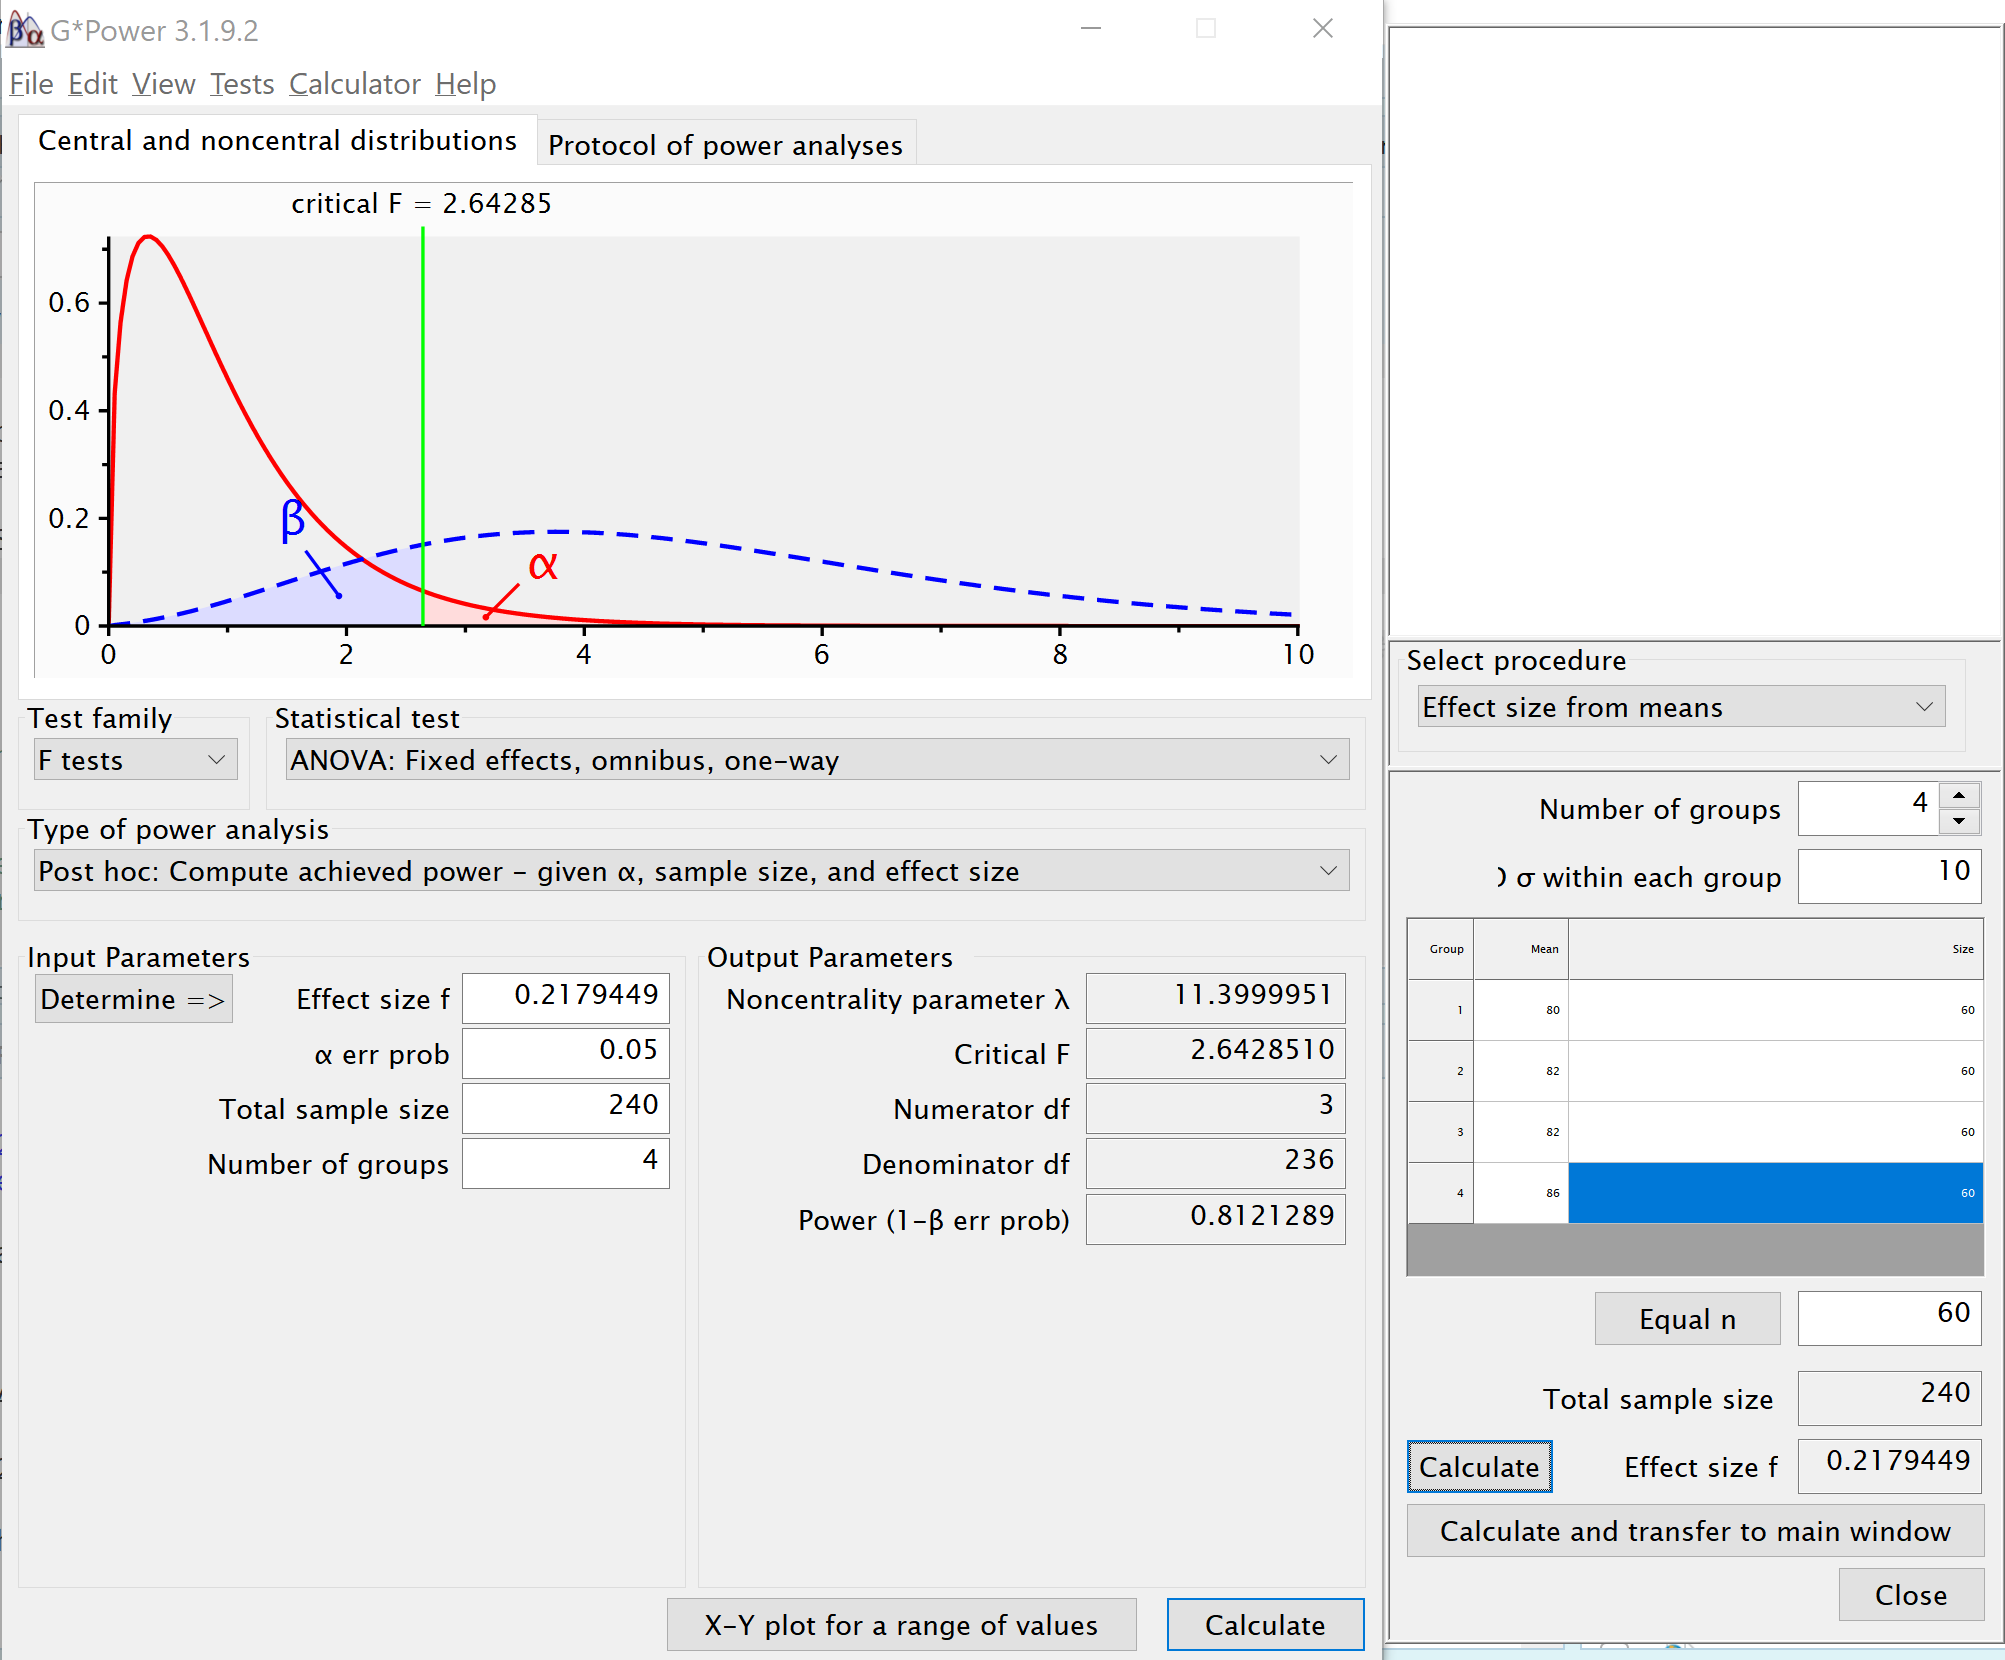
\includegraphics{screenshots/gpower_13.png}

\hypertarget{two-way-between-subject-interaction}{%
\section{Two-way Between Subject Interaction}\label{two-way-between-subject-interaction}}

\begin{Shaded}
\begin{Highlighting}[]
\NormalTok{string <-}\StringTok{ "2b*2b"}
\NormalTok{n <-}\StringTok{ }\DecValTok{20}
\NormalTok{mu <-}\StringTok{ }\KeywordTok{c}\NormalTok{(}\DecValTok{20}\NormalTok{, }\DecValTok{20}\NormalTok{, }\DecValTok{20}\NormalTok{, }\DecValTok{25}\NormalTok{) }
\CommentTok{# Enter means in the order that matches the labels below.}
\NormalTok{sd <-}\StringTok{ }\DecValTok{5}
\NormalTok{labelnames <-}\StringTok{ }\KeywordTok{c}\NormalTok{(}\StringTok{"A"}\NormalTok{, }\StringTok{"a1"}\NormalTok{, }\StringTok{"a2"}\NormalTok{, }\StringTok{"B"}\NormalTok{, }\StringTok{"b1"}\NormalTok{, }\StringTok{"b2"}\NormalTok{) }
\CommentTok{# the label names should be in the order of the means specified above.}

\NormalTok{design_result <-}\StringTok{ }\KeywordTok{ANOVA_design}\NormalTok{(}\DataTypeTok{design =}\NormalTok{ string,}
                   \DataTypeTok{n =}\NormalTok{ n, }
                   \DataTypeTok{mu =}\NormalTok{ mu, }
                   \DataTypeTok{sd =}\NormalTok{ sd, }
                   \DataTypeTok{labelnames =}\NormalTok{ labelnames)}



\NormalTok{exact_result <-}\StringTok{ }\KeywordTok{ANOVA_exact}\NormalTok{(design_result,}
                            \DataTypeTok{alpha_level =}\NormalTok{ alpha_level,}
                            \DataTypeTok{verbose =} \OtherTok{FALSE}\NormalTok{)}
\end{Highlighting}
\end{Shaded}

\begin{table}[!h]

\caption{\label{tab:unnamed-chunk-317}Exact ANOVA Result}
\centering
\begin{tabular}{l|r|r|r|r}
\hline
  & power & partial\_eta\_squared & cohen\_f & non\_centrality\\
\hline
A & 59.78655 & 0.0617284 & 0.2564946 & 5\\
\hline
B & 59.78655 & 0.0617284 & 0.2564946 & 5\\
\hline
A:B & 59.78655 & 0.0617284 & 0.2564946 & 5\\
\hline
\end{tabular}
\end{table}

\begin{Shaded}
\begin{Highlighting}[]
\CommentTok{#using default alpha level of .05}
\NormalTok{power_res <-}\StringTok{ }\KeywordTok{power_twoway_between}\NormalTok{(design_result) }
\NormalTok{power_res}\OperatorTok{$}\NormalTok{power_A}
\end{Highlighting}
\end{Shaded}

\begin{verbatim}
## [1] 59.78655
\end{verbatim}

\begin{Shaded}
\begin{Highlighting}[]
\NormalTok{power_res}\OperatorTok{$}\NormalTok{power_B}
\end{Highlighting}
\end{Shaded}

\begin{verbatim}
## [1] 59.78655
\end{verbatim}

\begin{Shaded}
\begin{Highlighting}[]
\NormalTok{power_res}\OperatorTok{$}\NormalTok{power_AB}
\end{Highlighting}
\end{Shaded}

\begin{verbatim}
## [1] 59.78655
\end{verbatim}

We can use the function by \citep{R-pwr2ppl}, as well.

\begin{Shaded}
\begin{Highlighting}[]
\KeywordTok{anova2x2}\NormalTok{(}\DataTypeTok{m1.1 =} \DecValTok{20}\NormalTok{,}
         \DataTypeTok{m1.2 =} \DecValTok{20}\NormalTok{,}
         \DataTypeTok{m2.1 =} \DecValTok{20}\NormalTok{,}
         \DataTypeTok{m2.2 =} \DecValTok{25}\NormalTok{,}
         \DataTypeTok{s1.1 =} \DecValTok{5}\NormalTok{,}
         \DataTypeTok{s1.2 =} \DecValTok{5}\NormalTok{,}
         \DataTypeTok{s2.1 =} \DecValTok{5}\NormalTok{,}
         \DataTypeTok{s2.2 =} \DecValTok{5}\NormalTok{,}
         \DataTypeTok{n1.1 =} \DecValTok{20}\NormalTok{,}
         \DataTypeTok{n1.2 =} \DecValTok{20}\NormalTok{,}
         \DataTypeTok{n2.1 =} \DecValTok{20}\NormalTok{,}
         \DataTypeTok{n2.2 =} \DecValTok{20}\NormalTok{,}
         \DataTypeTok{alpha =} \FloatTok{.05}\NormalTok{,}
         \DataTypeTok{all =} \StringTok{"OFF"}\NormalTok{)}
\end{Highlighting}
\end{Shaded}

\begin{verbatim}
## Power for Main Effect Factor A = 0.598
\end{verbatim}

\begin{verbatim}
## Power for Main Effect Factor B = 0.598
\end{verbatim}

\begin{verbatim}
## Power for Interaction AxB = 0.598
\end{verbatim}

\hypertarget{x3-between-subject-anova}{%
\section{3x3 Between Subject ANOVA}\label{x3-between-subject-anova}}

\begin{Shaded}
\begin{Highlighting}[]
\NormalTok{string <-}\StringTok{ "3b*3b"}
\NormalTok{n <-}\StringTok{ }\DecValTok{20}
\CommentTok{#All means are equal - so there is no real difference.}
\NormalTok{mu <-}\StringTok{ }\KeywordTok{c}\NormalTok{(}\DecValTok{20}\NormalTok{, }\DecValTok{20}\NormalTok{, }\DecValTok{20}\NormalTok{, }\DecValTok{20}\NormalTok{, }\DecValTok{20}\NormalTok{, }\DecValTok{20}\NormalTok{, }\DecValTok{20}\NormalTok{, }\DecValTok{20}\NormalTok{, }\DecValTok{25}\NormalTok{) }
\CommentTok{# Enter means in the order that matches the labels below.}
\NormalTok{sd <-}\StringTok{ }\DecValTok{5}
\NormalTok{labelnames <-}\StringTok{ }\KeywordTok{c}\NormalTok{(}\StringTok{"Factor_A"}\NormalTok{, }\StringTok{"a1"}\NormalTok{, }\StringTok{"a2"}\NormalTok{, }\StringTok{"a3"}\NormalTok{, }\StringTok{"Factor_B"}\NormalTok{, }\StringTok{"b1"}\NormalTok{, }\StringTok{"b2"}\NormalTok{, }\StringTok{"b3"}\NormalTok{) }
\CommentTok{# the label names should be in the order of the means specified above.}
\NormalTok{design_result <-}\StringTok{ }\KeywordTok{ANOVA_design}\NormalTok{(}\DataTypeTok{design =}\NormalTok{ string,}
                   \DataTypeTok{n =}\NormalTok{ n, }
                   \DataTypeTok{mu =}\NormalTok{ mu, }
                   \DataTypeTok{sd =}\NormalTok{ sd, }
                   \DataTypeTok{labelnames =}\NormalTok{ labelnames)}



\NormalTok{exact_result <-}\StringTok{ }\KeywordTok{ANOVA_exact}\NormalTok{(design_result,}
                            \DataTypeTok{alpha_level =}\NormalTok{ alpha_level,}
                            \DataTypeTok{verbose =} \OtherTok{FALSE}\NormalTok{)}
\end{Highlighting}
\end{Shaded}

\begin{table}[!h]

\caption{\label{tab:unnamed-chunk-321}Exact ANOVA Result}
\centering
\begin{tabular}{l|r|r|r|r}
\hline
  & power & partial\_eta\_squared & cohen\_f & non\_centrality\\
\hline
Factor\_A & 44.86306 & 0.0253325 & 0.1612169 & 4.444444\\
\hline
Factor\_B & 44.86306 & 0.0253325 & 0.1612169 & 4.444444\\
\hline
Factor\_A:Factor\_B & 64.34127 & 0.0494132 & 0.2279952 & 8.888889\\
\hline
\end{tabular}
\end{table}

\begin{Shaded}
\begin{Highlighting}[]
\CommentTok{#using default alpha level of .05}
\NormalTok{power_res <-}\StringTok{ }\KeywordTok{power_twoway_between}\NormalTok{(design_result) }
\NormalTok{power_res}\OperatorTok{$}\NormalTok{power_A}
\end{Highlighting}
\end{Shaded}

\begin{verbatim}
## [1] 44.86306
\end{verbatim}

\begin{Shaded}
\begin{Highlighting}[]
\NormalTok{power_res}\OperatorTok{$}\NormalTok{power_B}
\end{Highlighting}
\end{Shaded}

\begin{verbatim}
## [1] 44.86306
\end{verbatim}

\begin{Shaded}
\begin{Highlighting}[]
\NormalTok{power_res}\OperatorTok{$}\NormalTok{power_AB}
\end{Highlighting}
\end{Shaded}

\begin{verbatim}
## [1] 64.34127
\end{verbatim}

\hypertarget{power-curve}{%
\chapter{Power Curve}\label{power-curve}}

Power is calculated for a specific value of an effect size, alpha level, and sample size. Because you often do not know the true effect size, it often makes more sense to think of the power curve as a function of the size of the effect. Although power curves could be constructed from Monte Carlo simulations (\texttt{ANOVA\_power}) the \texttt{plot\_power} function utilizes the \texttt{ANOVA\_exact} function within its code because these ``exact'' simulations are much faster. The basic approach is to calculate power for a specific pattern of means, a specific effect size, a given alpha level, and a specific pattern of correlations. This is one example:

\begin{Shaded}
\begin{Highlighting}[]
\CommentTok{#2x2 design}
\NormalTok{string =}\StringTok{ "2w*2w"}
\NormalTok{mu =}\StringTok{ }\KeywordTok{c}\NormalTok{(}\DecValTok{0}\NormalTok{,}\DecValTok{0}\NormalTok{,}\DecValTok{0}\NormalTok{,}\FloatTok{0.5}\NormalTok{)}
\NormalTok{n <-}\StringTok{ }\DecValTok{20}
\NormalTok{sd <-}\StringTok{ }\DecValTok{1}
\NormalTok{r <-}\StringTok{ }\FloatTok{0.5}
\NormalTok{labelnames =}\StringTok{ }\KeywordTok{c}\NormalTok{(}\StringTok{"A"}\NormalTok{, }\StringTok{"a1"}\NormalTok{, }\StringTok{"a2"}\NormalTok{, }\StringTok{"B"}\NormalTok{, }\StringTok{"b1"}\NormalTok{, }\StringTok{"b2"}\NormalTok{)}

\NormalTok{design_result <-}\StringTok{ }\KeywordTok{ANOVA_design}\NormalTok{(}\DataTypeTok{design =}\NormalTok{ string,}
                              \DataTypeTok{n =}\NormalTok{ n, }
                              \DataTypeTok{mu =}\NormalTok{ mu, }
                              \DataTypeTok{sd =}\NormalTok{ sd, }
                              \DataTypeTok{r =}\NormalTok{ r, }
                              \DataTypeTok{labelnames =}\NormalTok{ labelnames)}

\NormalTok{exact_result <-}\StringTok{ }\KeywordTok{ANOVA_exact}\NormalTok{(design_result,}
                            \DataTypeTok{alpha_level =}\NormalTok{ alpha_level,}
                            \DataTypeTok{verbose =} \OtherTok{FALSE}\NormalTok{)}
\end{Highlighting}
\end{Shaded}

\begin{table}[!h]

\caption{\label{tab:unnamed-chunk-325}Exact ANOVA Result}
\centering
\begin{tabular}{l|r|r|r|r}
\hline
  & power & partial\_eta\_squared & cohen\_f & non\_centrality\\
\hline
A & 32.35926 & 0.1162791 & 0.3627381 & 2.5\\
\hline
B & 32.35926 & 0.1162791 & 0.3627381 & 2.5\\
\hline
A:B & 32.35926 & 0.1162791 & 0.3627381 & 2.5\\
\hline
\end{tabular}
\end{table}
\pagebreak

We can make these calculations for a range of sample sizes, to get a power curve. We created a simple function that performs these calculations across a range of sample sizes (from n = 3 to max\_, a variable you can specify in the function).

\begin{Shaded}
\begin{Highlighting}[]
\NormalTok{p_a <-}\StringTok{ }\KeywordTok{plot_power}\NormalTok{(design_result,}
                      \DataTypeTok{max_n =} \DecValTok{50}\NormalTok{)}
\NormalTok{p_a}\OperatorTok{$}\NormalTok{plot_ANOVA}
\end{Highlighting}
\end{Shaded}

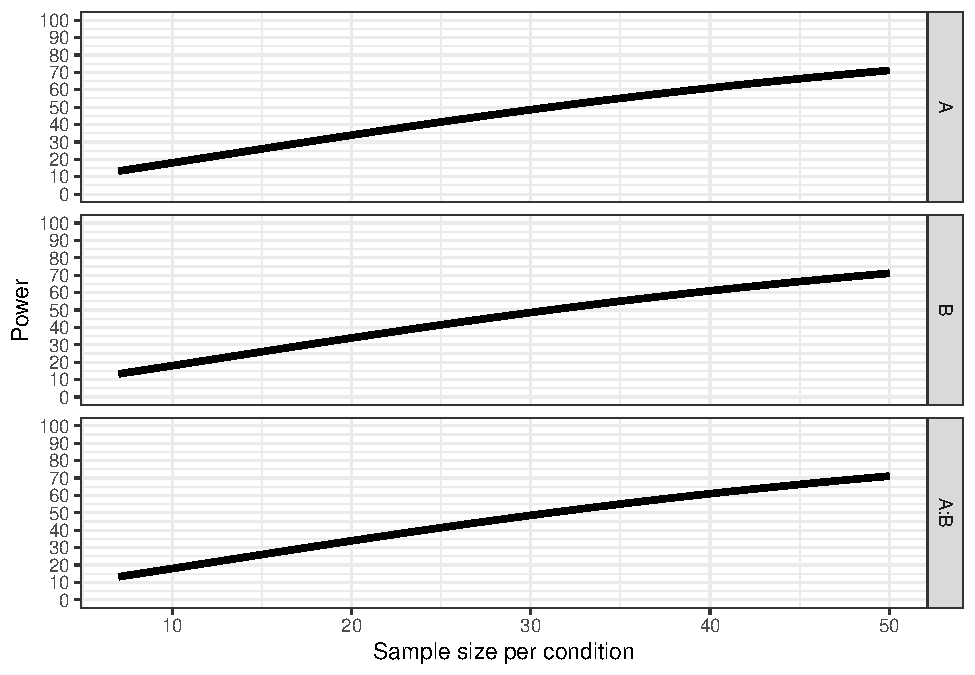
\includegraphics{SuperpowerValidation_files/figure-latex/unnamed-chunk-326-1.pdf}

If we run many of these \texttt{plot\_power} functions across small changes in the ANOVA\_design we can compile a number of power curves that can be combined into a single plot. We do this below. The code to reprodcue these plots can be found on the \href{https://github.com/arcaldwell49/SuperpowerBook/tree/master/data}{GitHub repository for this book}.
\pagebreak

\hypertarget{explore-increase-in-effect-size-for-moderated-interactions.}{%
\section{Explore increase in effect size for moderated interactions.}\label{explore-increase-in-effect-size-for-moderated-interactions.}}

The design has means 0, 0, 0, 0, with one cell increasing by 0.1, up to 0, 0, 0, 0.5. The standard deviation is set to 1. The correlation between all variables is 0.5.

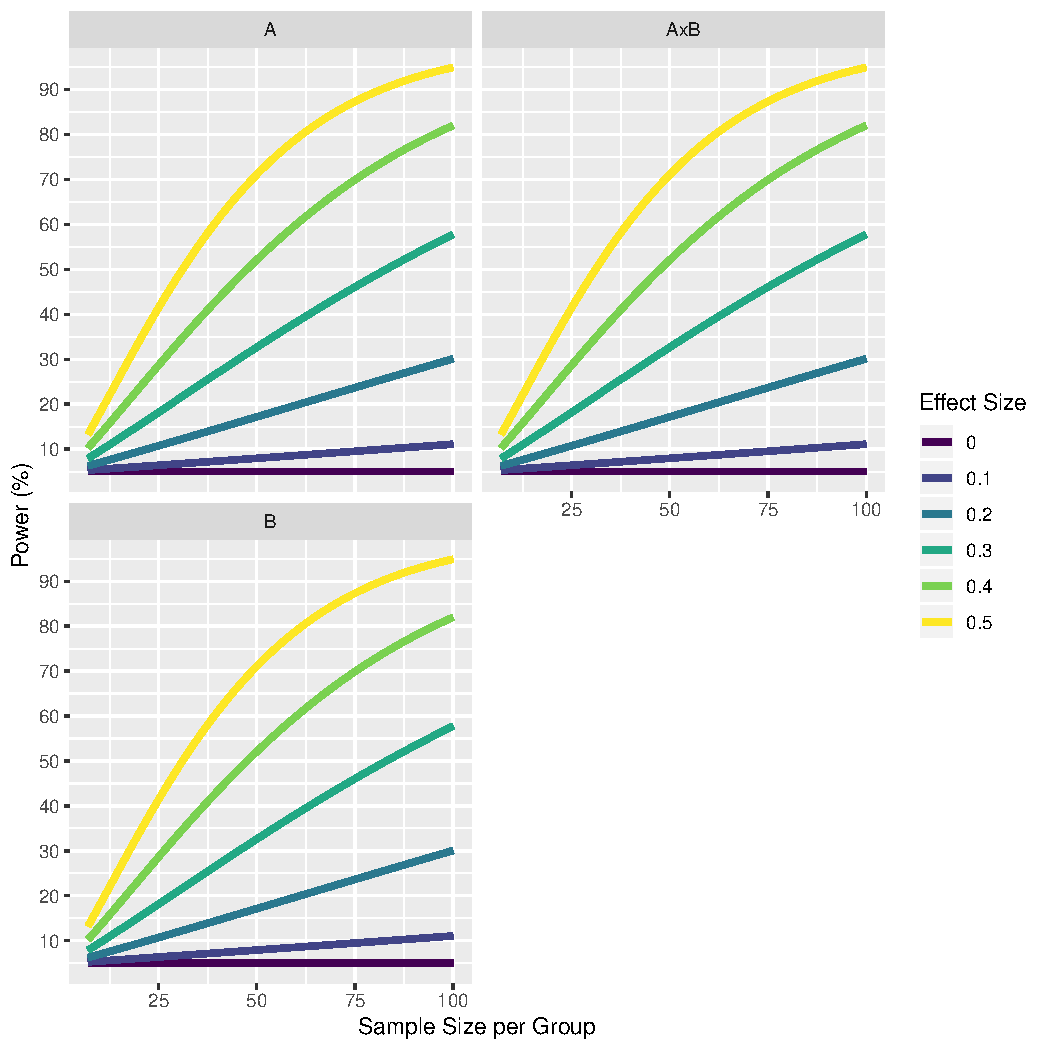
\includegraphics{SuperpowerValidation_files/figure-latex/unnamed-chunk-327-1.pdf}
\pagebreak

\hypertarget{explore-increase-in-effect-size-for-cross-over-interactions.}{%
\section{Explore increase in effect size for cross-over interactions.}\label{explore-increase-in-effect-size-for-cross-over-interactions.}}

The design has means 0, 0, 0, 0, with two cells increasing by 0.1, up to 0.5, 0, 0, 0.5. The standard deviation is set to 1. The correlation between all variables is 0.5.

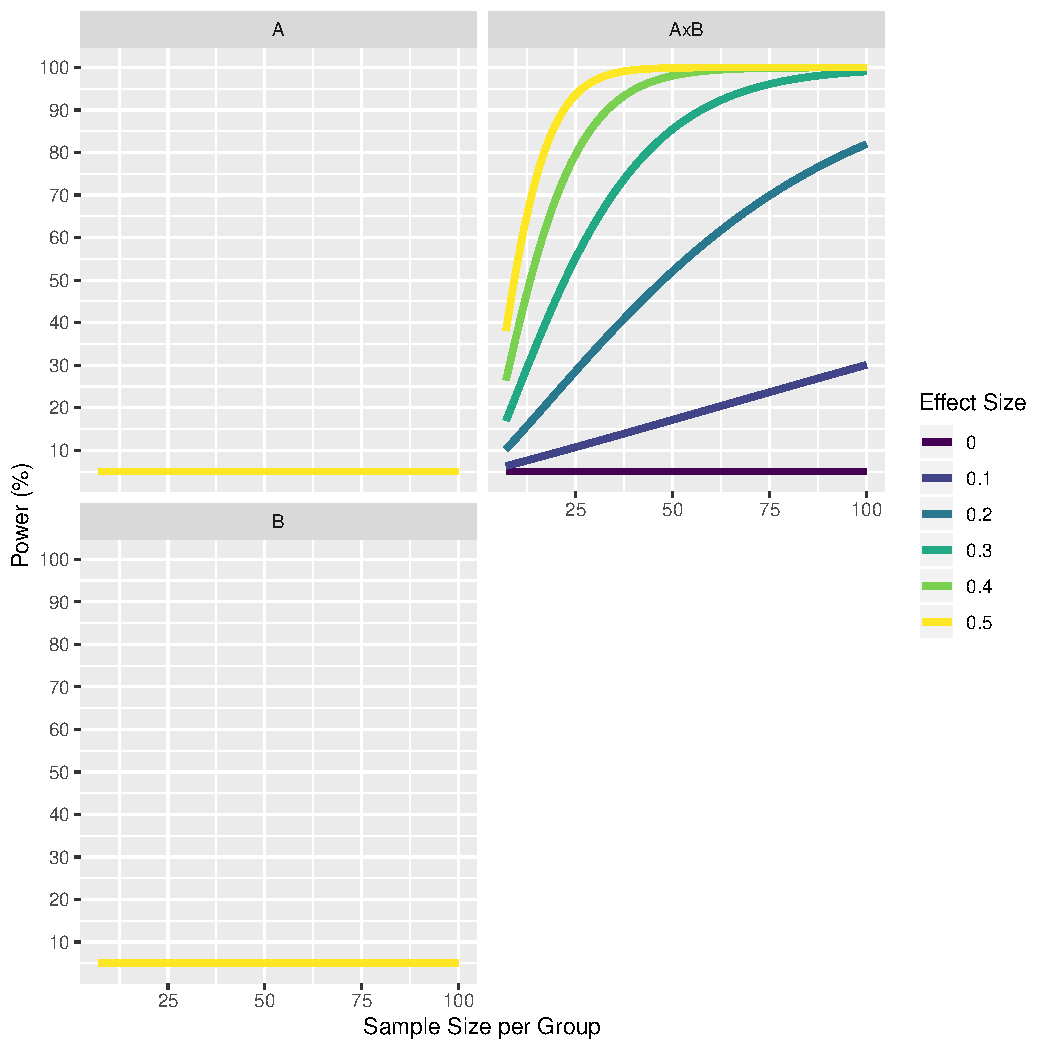
\includegraphics{SuperpowerValidation_files/figure-latex/unnamed-chunk-328-1.pdf}
\pagebreak

\hypertarget{explore-increase-in-correlation-in-moderated-interactions.}{%
\section{Explore increase in correlation in moderated interactions.}\label{explore-increase-in-correlation-in-moderated-interactions.}}

The design has means 0, 0, 0, 0.3. The standard deviation is set to 1. The correlation between all variables increases from 0 to 0.9.

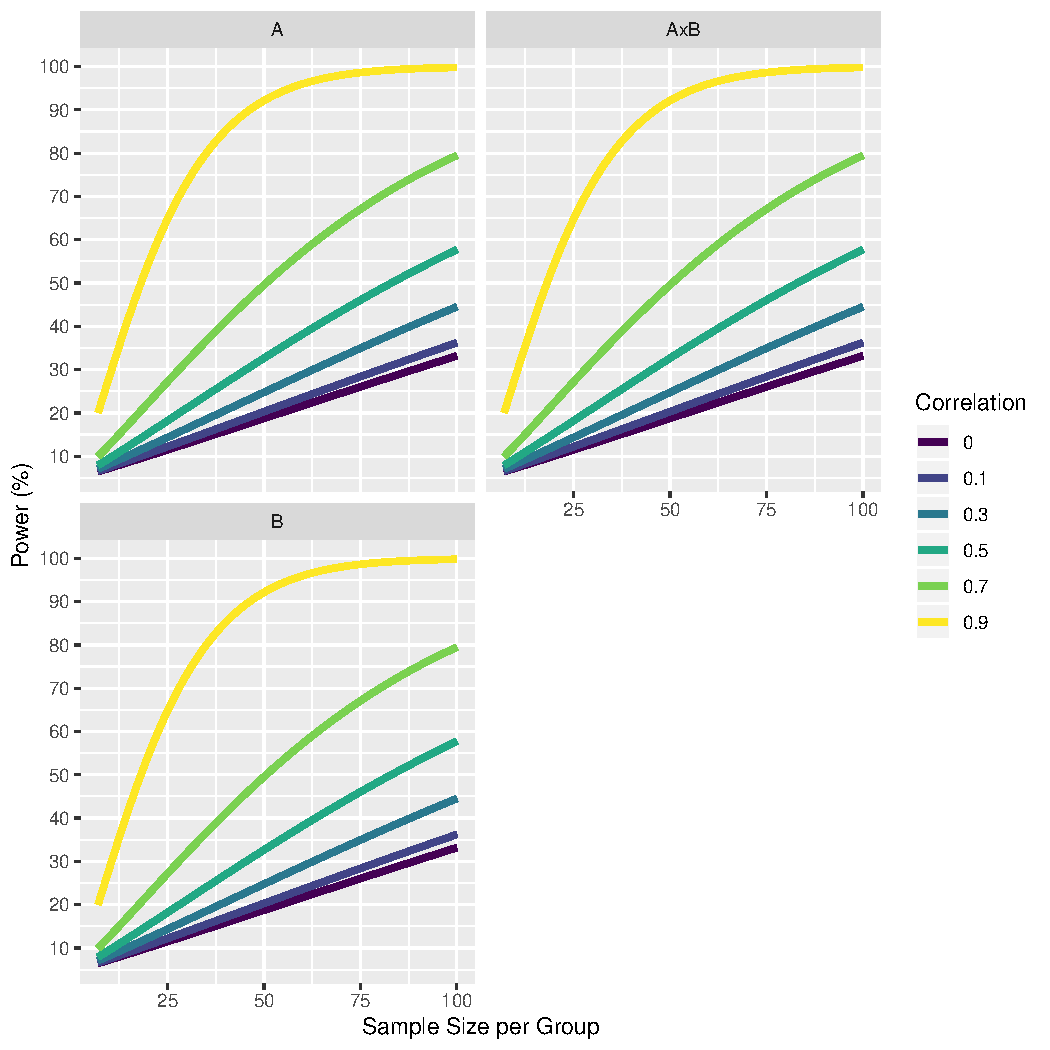
\includegraphics{SuperpowerValidation_files/figure-latex/unnamed-chunk-329-1.pdf}
\pagebreak

\hypertarget{increasing-correlation-in-on-factor-decreases-power-in-second-factor}{%
\section{Increasing correlation in on factor decreases power in second factor}\label{increasing-correlation-in-on-factor-decreases-power-in-second-factor}}

As \citet{potvin2000statistical} write:

\begin{quote}
The more important finding with respect to the effect of \emph{r} on power relates to the effect of the correlations associated with one factor on the power of the test of the main effect of the other factor. Specifically, if the correlations among the levels of B are larger than those within the AB matrix (i.e., \emph{r}(B) - \emph{r}(AB) \textgreater{} 0.0), there is a reduction in the power for the test of the A effect (and the test on B is similarly affected by the A correlations).
\end{quote}

We see this in the plots below. As the correlation of the A factor increases from 0.4 to 0.9, we see the power for the main effect decreases.

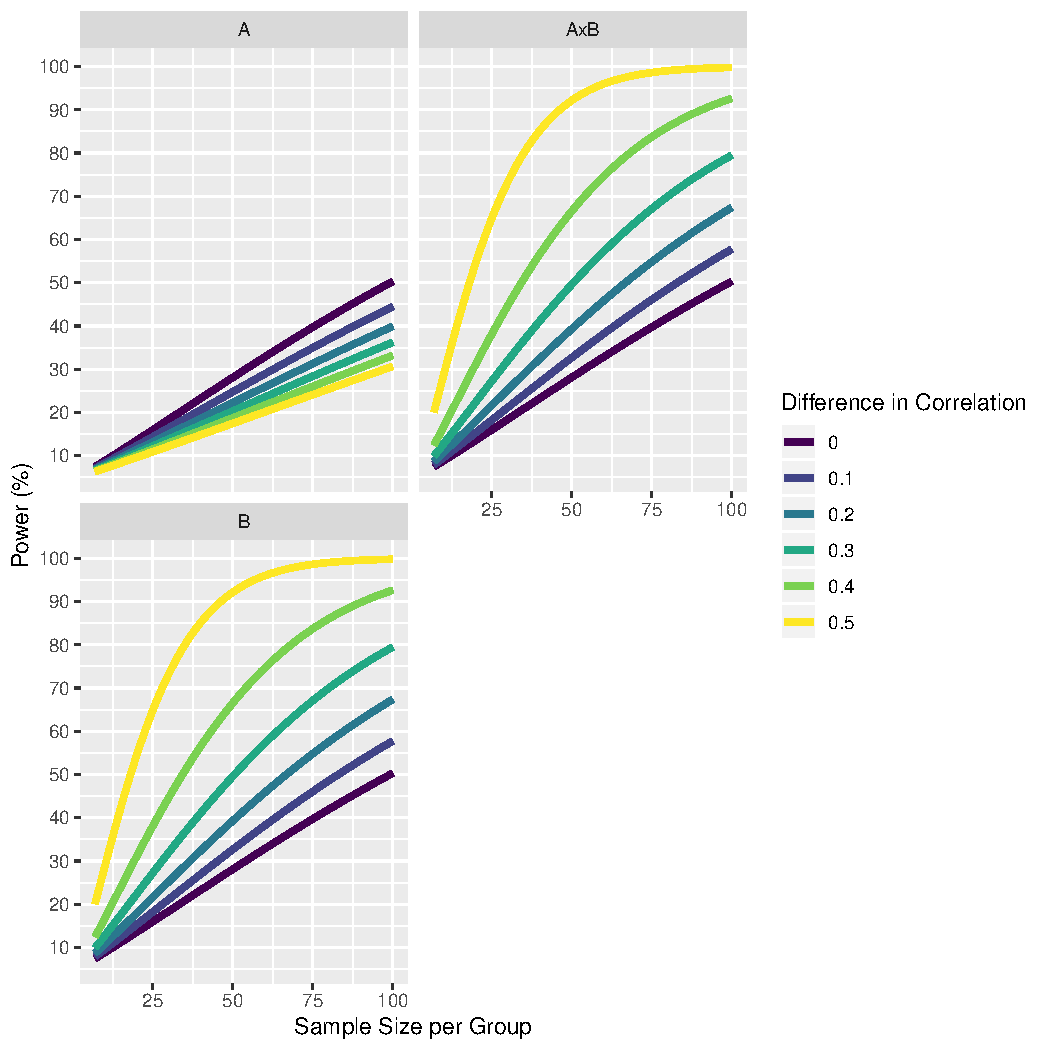
\includegraphics{SuperpowerValidation_files/figure-latex/unnamed-chunk-330-1.pdf}

\hypertarget{appendix-1-direct-comparison-to-pwr2ppl}{%
\chapter*{Appendix 1: Direct Comparison to pwr2ppl}\label{appendix-1-direct-comparison-to-pwr2ppl}}
\addcontentsline{toc}{chapter}{Appendix 1: Direct Comparison to pwr2ppl}

In this appendix we have included the performance of \texttt{Superpower} to the \texttt{pwr2ppl} package using Chris Aberson's examples in \href{https://www.crcpress.com/Applied-Power-Analysis-for-the-Behavioral-Sciences-2nd-Edition/Aberson/p/book/9781138044593}{\emph{Applied Power Analysis for the Behavioral Sciences}} (2nd edition).

\hypertarget{examples-from-chapter-5}{%
\section{Examples from Chapter 5}\label{examples-from-chapter-5}}

\hypertarget{example-5.15.2}{%
\subsection{Example 5.1/5.2}\label{example-5.15.2}}

In this example, Aberson proposes a study expecting an average ``score'' of 80, 82, 82, and 86 for the control and three treatment groups respectively. The common standard deviation is 10 and the sample size per cell is 60.

\begin{Shaded}
\begin{Highlighting}[]
\NormalTok{design_result <-}\StringTok{ }\KeywordTok{ANOVA_design}\NormalTok{(}\DataTypeTok{design =} \StringTok{"4b"}\NormalTok{,}
                              \DataTypeTok{n =} \DecValTok{60}\NormalTok{,}
                              \DataTypeTok{sd =} \DecValTok{10}\NormalTok{,}
                              \DataTypeTok{mu =} \KeywordTok{c}\NormalTok{(}\DecValTok{80}\NormalTok{, }\DecValTok{82}\NormalTok{, }\DecValTok{82}\NormalTok{, }\DecValTok{86}\NormalTok{),}
                              \DataTypeTok{labelnames =} \KeywordTok{c}\NormalTok{(}\StringTok{"DORM"}\NormalTok{,}
                              \StringTok{"Control"}\NormalTok{,}
                              \StringTok{"T1"}\NormalTok{,}
                              \StringTok{"T2"}\NormalTok{,}
                              \StringTok{"T3"}\NormalTok{),}
                              \DataTypeTok{plot =} \OtherTok{TRUE}\NormalTok{)}
\end{Highlighting}
\end{Shaded}

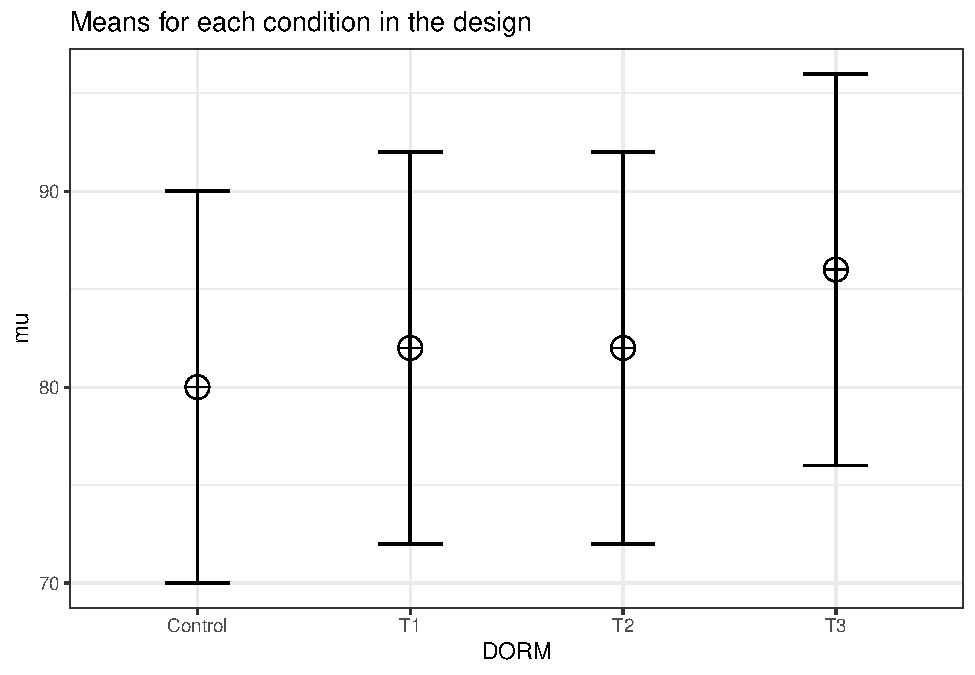
\includegraphics{SuperpowerValidation_files/figure-latex/aberson_appendix-1.pdf}

Now we calculate the analytical result from \texttt{Superpower}.

\begin{Shaded}
\begin{Highlighting}[]
\NormalTok{analytical_result <-}\StringTok{ }\KeywordTok{power_oneway_between}\NormalTok{(design_result)}

\NormalTok{analytical_result}\OperatorTok{$}\NormalTok{power}
\end{Highlighting}
\end{Shaded}

\begin{verbatim}
## [1] 81.21291
\end{verbatim}

The \texttt{ANOVA\_exact} result.

\begin{Shaded}
\begin{Highlighting}[]
\NormalTok{exact_result <-}\StringTok{ }\KeywordTok{ANOVA_exact}\NormalTok{(design_result, }\DataTypeTok{verbose =} \OtherTok{FALSE}\NormalTok{)}

\NormalTok{exact_result}\OperatorTok{$}\NormalTok{main_results}
\end{Highlighting}
\end{Shaded}

\begin{verbatim}
##         power partial_eta_squared   cohen_f non_centrality
## DORM 81.21291          0.04607922 0.2197842           11.4
\end{verbatim}

And these match \texttt{pwr2ppl}.

\begin{Shaded}
\begin{Highlighting}[]
\KeywordTok{anova1f_4}\NormalTok{(}\DataTypeTok{m1 =} \DecValTok{80}\NormalTok{, }\DataTypeTok{m2 =} \DecValTok{82}\NormalTok{, }\DataTypeTok{m3 =} \DecValTok{82}\NormalTok{, }\DataTypeTok{m4 =} \DecValTok{86}\NormalTok{,}
          \DataTypeTok{s1 =} \DecValTok{10}\NormalTok{, }\DataTypeTok{s2 =} \DecValTok{10}\NormalTok{, }\DataTypeTok{s3 =} \DecValTok{10}\NormalTok{, }\DataTypeTok{s4 =} \DecValTok{10}\NormalTok{,}
          \DataTypeTok{n1 =} \DecValTok{60}\NormalTok{, }\DataTypeTok{n2 =} \DecValTok{60}\NormalTok{, }\DataTypeTok{n3 =} \DecValTok{60}\NormalTok{, }\DataTypeTok{n4 =} \DecValTok{60}\NormalTok{)}
\end{Highlighting}
\end{Shaded}

\begin{verbatim}
## Power  = 0.812 for eta-squared = 0.05
\end{verbatim}

\hypertarget{example-5.3}{%
\subsection{Example 5.3}\label{example-5.3}}

Now a 2 x 2 between-subject ANOVA.

\begin{Shaded}
\begin{Highlighting}[]
\NormalTok{design_result <-}\StringTok{ }\KeywordTok{ANOVA_design}\NormalTok{(}\DataTypeTok{design =} \StringTok{"2b*2b"}\NormalTok{,}
                              \DataTypeTok{n =} \DecValTok{100}\NormalTok{,}
                              \DataTypeTok{sd =} \FloatTok{1.7}\NormalTok{,}
                              \DataTypeTok{mu =} \KeywordTok{c}\NormalTok{(.}\DecValTok{85}\NormalTok{, }\FloatTok{.85}\NormalTok{, }
                                     \DecValTok{0}\NormalTok{, }\FloatTok{.6}\NormalTok{),}
                              \DataTypeTok{plot =} \OtherTok{TRUE}\NormalTok{)}
\end{Highlighting}
\end{Shaded}

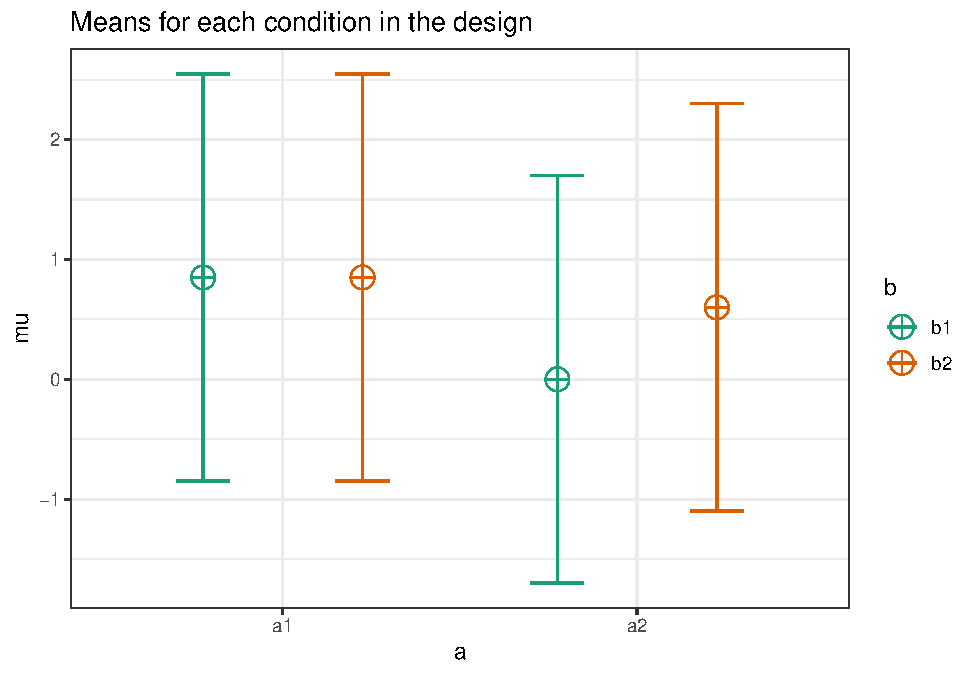
\includegraphics{SuperpowerValidation_files/figure-latex/aberson_5.3.2-1.pdf}

Now we calculate the analytical result from \texttt{Superpower}.

\begin{Shaded}
\begin{Highlighting}[]
\NormalTok{analytical_result <-}\StringTok{ }\KeywordTok{power_twoway_between}\NormalTok{(design_result)}

\NormalTok{analytical_result}\OperatorTok{$}\NormalTok{power_A}
\end{Highlighting}
\end{Shaded}

\begin{verbatim}
## [1] 89.75072
\end{verbatim}

\begin{Shaded}
\begin{Highlighting}[]
\NormalTok{analytical_result}\OperatorTok{$}\NormalTok{power_B}
\end{Highlighting}
\end{Shaded}

\begin{verbatim}
## [1] 42.10204
\end{verbatim}

\begin{Shaded}
\begin{Highlighting}[]
\NormalTok{analytical_result}\OperatorTok{$}\NormalTok{power_AB}
\end{Highlighting}
\end{Shaded}

\begin{verbatim}
## [1] 42.10204
\end{verbatim}

The \texttt{ANOVA\_exact} result.

\begin{Shaded}
\begin{Highlighting}[]
\NormalTok{exact_result <-}\StringTok{ }\KeywordTok{ANOVA_exact}\NormalTok{(design_result, }\DataTypeTok{verbose =} \OtherTok{FALSE}\NormalTok{)}

\NormalTok{exact_result}\OperatorTok{$}\NormalTok{main_results}
\end{Highlighting}
\end{Shaded}

\begin{verbatim}
##        power partial_eta_squared    cohen_f non_centrality
## a   89.75072         0.025751475 0.16257965      10.467128
## b   42.10204         0.007802747 0.08867981       3.114187
## a:b 42.10204         0.007802747 0.08867981       3.114187
\end{verbatim}

And these match \texttt{pwr2ppl}. From Table 5.12.

\begin{Shaded}
\begin{Highlighting}[]
\KeywordTok{anova2x2}\NormalTok{(}\DataTypeTok{m1.1 =} \FloatTok{0.85}\NormalTok{, }\DataTypeTok{m1.2 =} \FloatTok{0.85}\NormalTok{, }\DataTypeTok{m2.1 =} \FloatTok{0.00}\NormalTok{, }\DataTypeTok{m2.2 =} \FloatTok{0.60}\NormalTok{,}
         \DataTypeTok{s1.1 =} \FloatTok{1.7}\NormalTok{, }\DataTypeTok{s1.2 =} \FloatTok{1.7}\NormalTok{, }\DataTypeTok{s2.1 =} \FloatTok{1.7}\NormalTok{, }\DataTypeTok{s2.2 =} \FloatTok{1.7}\NormalTok{,}
         \DataTypeTok{n1.1 =} \DecValTok{100}\NormalTok{, }\DataTypeTok{n1.2 =} \DecValTok{100}\NormalTok{, }\DataTypeTok{n2.1 =} \DecValTok{100}\NormalTok{, }\DataTypeTok{n2.2 =} \DecValTok{100}\NormalTok{,}
         \DataTypeTok{alpha =} \FloatTok{.05}\NormalTok{)}
\end{Highlighting}
\end{Shaded}

\begin{verbatim}
## Power for Main Effect Factor A = 0.898
\end{verbatim}

\begin{verbatim}
## Power for Main Effect Factor B = 0.421
\end{verbatim}

\begin{verbatim}
## Power for Interaction AxB = 0.421
\end{verbatim}

Now we can increase the sample size to 250 per cell

\begin{Shaded}
\begin{Highlighting}[]
\NormalTok{design_result <-}\StringTok{ }\KeywordTok{ANOVA_design}\NormalTok{(}\DataTypeTok{design =} \StringTok{"2b*2b"}\NormalTok{,}
                              \DataTypeTok{n =} \DecValTok{250}\NormalTok{,}
                              \DataTypeTok{sd =} \FloatTok{1.7}\NormalTok{,}
                              \DataTypeTok{mu =} \KeywordTok{c}\NormalTok{(.}\DecValTok{85}\NormalTok{, }\FloatTok{.85}\NormalTok{, }
                                     \DecValTok{0}\NormalTok{, }\FloatTok{.6}\NormalTok{),}
                              \DataTypeTok{plot =} \OtherTok{TRUE}\NormalTok{)}
\end{Highlighting}
\end{Shaded}

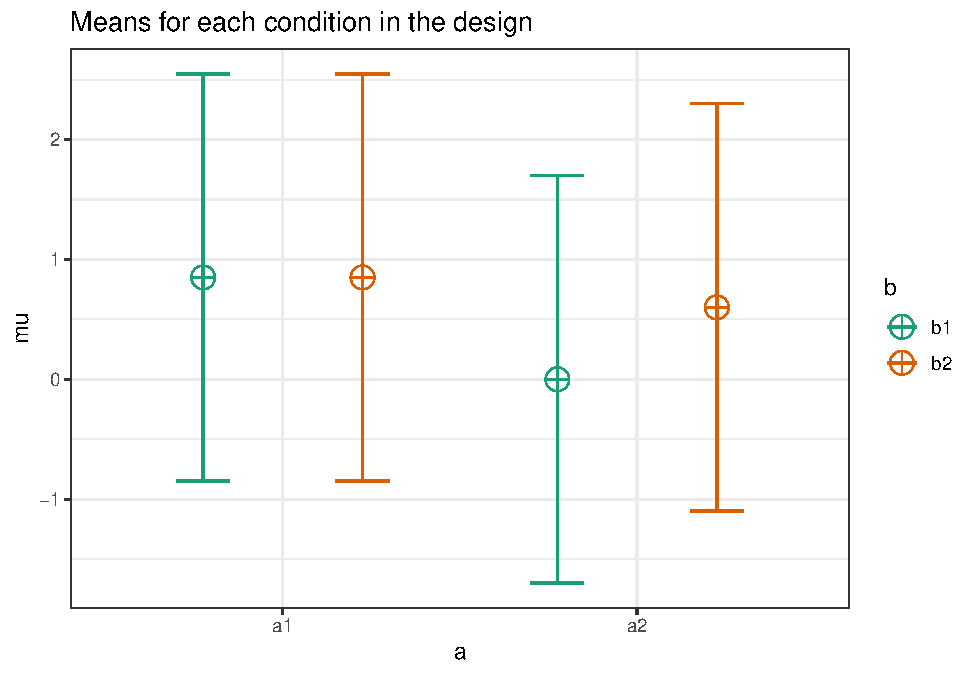
\includegraphics{SuperpowerValidation_files/figure-latex/aberson_5.3-1.pdf}

Now we calculate the analytical result from \texttt{Superpower}.

\begin{Shaded}
\begin{Highlighting}[]
\NormalTok{analytical_result <-}\StringTok{ }\KeywordTok{power_twoway_between}\NormalTok{(design_result)}

\NormalTok{analytical_result}\OperatorTok{$}\NormalTok{power_A}
\end{Highlighting}
\end{Shaded}

\begin{verbatim}
## [1] 99.91852
\end{verbatim}

\begin{Shaded}
\begin{Highlighting}[]
\NormalTok{analytical_result}\OperatorTok{$}\NormalTok{power_B}
\end{Highlighting}
\end{Shaded}

\begin{verbatim}
## [1] 79.60496
\end{verbatim}

\begin{Shaded}
\begin{Highlighting}[]
\NormalTok{analytical_result}\OperatorTok{$}\NormalTok{power_AB}
\end{Highlighting}
\end{Shaded}

\begin{verbatim}
## [1] 79.60496
\end{verbatim}

The \texttt{ANOVA\_exact} result.

\begin{Shaded}
\begin{Highlighting}[]
\NormalTok{exact_result <-}\StringTok{ }\KeywordTok{ANOVA_exact}\NormalTok{(design_result, }\DataTypeTok{verbose =} \OtherTok{FALSE}\NormalTok{)}

\NormalTok{exact_result}\OperatorTok{$}\NormalTok{main_results}
\end{Highlighting}
\end{Shaded}

\begin{verbatim}
##        power partial_eta_squared   cohen_f non_centrality
## a   99.91852         0.025600317 0.1620892      26.167820
## b   79.60496         0.007756107 0.0884123       7.785467
## a:b 79.60496         0.007756107 0.0884123       7.785467
\end{verbatim}

And these match \texttt{pwr2ppl}.

\begin{Shaded}
\begin{Highlighting}[]
\KeywordTok{anova2x2}\NormalTok{(}\DataTypeTok{m1.1 =} \FloatTok{0.85}\NormalTok{, }\DataTypeTok{m1.2 =} \FloatTok{0.85}\NormalTok{, }\DataTypeTok{m2.1 =} \FloatTok{0.00}\NormalTok{, }\DataTypeTok{m2.2 =} \FloatTok{0.60}\NormalTok{,}
         \DataTypeTok{s1.1 =} \FloatTok{1.7}\NormalTok{, }\DataTypeTok{s1.2 =} \FloatTok{1.7}\NormalTok{, }\DataTypeTok{s2.1 =} \FloatTok{1.7}\NormalTok{, }\DataTypeTok{s2.2 =} \FloatTok{1.7}\NormalTok{,}
         \DataTypeTok{n1.1 =} \DecValTok{250}\NormalTok{, }\DataTypeTok{n1.2 =} \DecValTok{250}\NormalTok{, }\DataTypeTok{n2.1 =} \DecValTok{250}\NormalTok{, }\DataTypeTok{n2.2 =} \DecValTok{250}\NormalTok{,}
         \DataTypeTok{alpha =} \FloatTok{.05}\NormalTok{)}
\end{Highlighting}
\end{Shaded}

\begin{verbatim}
## Power for Main Effect Factor A = 0.999
\end{verbatim}

\begin{verbatim}
## Power for Main Effect Factor B = 0.796
\end{verbatim}

\begin{verbatim}
## Power for Interaction AxB = 0.796
\end{verbatim}

\hypertarget{examples-from-chapter-6}{%
\section{Examples from Chapter 6}\label{examples-from-chapter-6}}

Repeated measures ANOVAs

\hypertarget{example-from-table-6.2}{%
\subsection{Example from Table 6.2}\label{example-from-table-6.2}}

\begin{Shaded}
\begin{Highlighting}[]
\NormalTok{design_result <-}\StringTok{ }\KeywordTok{ANOVA_design}\NormalTok{(}\DataTypeTok{design =} \StringTok{"4w"}\NormalTok{,}
                              \DataTypeTok{n =} \DecValTok{25}\NormalTok{,}
                              \DataTypeTok{sd =} \KeywordTok{c}\NormalTok{(.}\DecValTok{4}\NormalTok{,.}\DecValTok{5}\NormalTok{,.}\DecValTok{6}\NormalTok{,.}\DecValTok{7}\NormalTok{),}
                              \DataTypeTok{mu =} \KeywordTok{c}\NormalTok{(}\OperatorTok{-}\NormalTok{.}\DecValTok{25}\NormalTok{, }\FloatTok{.00}\NormalTok{, }\FloatTok{.10}\NormalTok{, }\FloatTok{.15}\NormalTok{),}
                              \DataTypeTok{r =} \KeywordTok{c}\NormalTok{(.}\DecValTok{50}\NormalTok{, }
                                    \FloatTok{.30}\NormalTok{,}
                                    \FloatTok{.15}\NormalTok{, }
                                    \FloatTok{.5}\NormalTok{,}
                                    \FloatTok{.30}\NormalTok{, }
                                    \FloatTok{.50}\NormalTok{),}
                              \DataTypeTok{plot =} \OtherTok{TRUE}\NormalTok{)}
\end{Highlighting}
\end{Shaded}

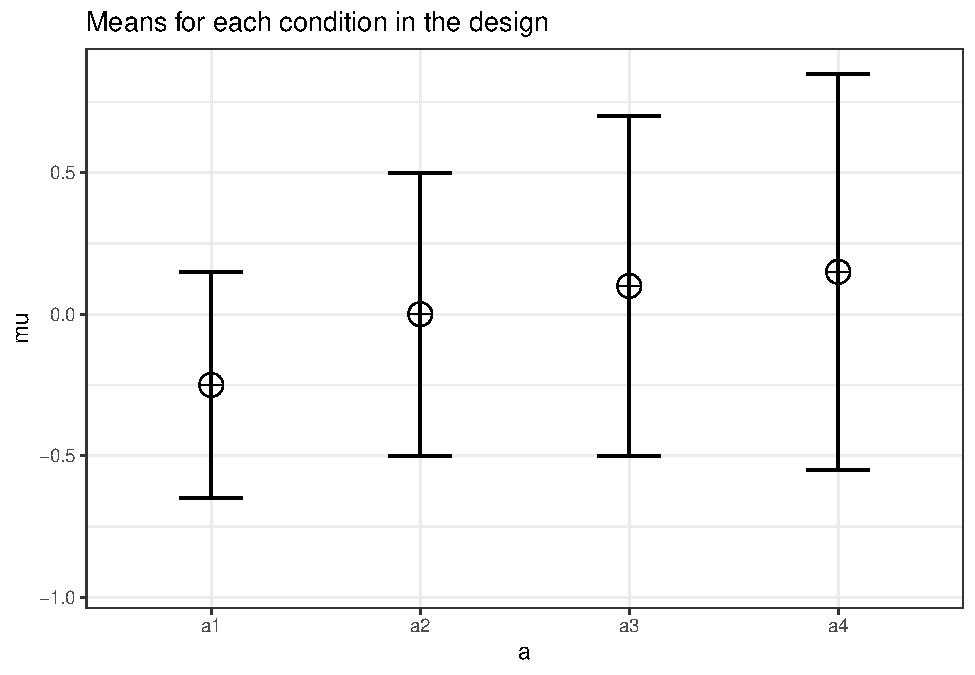
\includegraphics{SuperpowerValidation_files/figure-latex/aberson_6.2-1.pdf}

\begin{Shaded}
\begin{Highlighting}[]
\NormalTok{design_result}\OperatorTok{$}\NormalTok{cor_mat}
\end{Highlighting}
\end{Shaded}

\begin{verbatim}
##      a1  a2  a3   a4
## a1 1.00 0.5 0.3 0.15
## a2 0.50 1.0 0.5 0.30
## a3 0.30 0.5 1.0 0.50
## a4 0.15 0.3 0.5 1.00
\end{verbatim}

There is no analytical result from \texttt{Superpower} when the correlations vary.

Now we prouce 3 \texttt{ANOVA\_exact} results representing no sphericity correction, Greenhouse-Geisser, and Huynh-Feldt corrected results.

\begin{Shaded}
\begin{Highlighting}[]
\NormalTok{exact_result <-}\StringTok{ }\KeywordTok{ANOVA_exact}\NormalTok{(design_result, }\DataTypeTok{verbose =} \OtherTok{FALSE}\NormalTok{)}

\NormalTok{exact_result}\OperatorTok{$}\NormalTok{main_results}
\end{Highlighting}
\end{Shaded}

\begin{verbatim}
##      power partial_eta_squared   cohen_f non_centrality
## a 80.94999           0.1404744 0.4042678       11.76713
\end{verbatim}

\begin{Shaded}
\begin{Highlighting}[]
\NormalTok{exact_result <-}\StringTok{ }\KeywordTok{ANOVA_exact}\NormalTok{(design_result,}
                            \DataTypeTok{correction =} \StringTok{"GG"}\NormalTok{,}
                            \DataTypeTok{verbose =} \OtherTok{FALSE}\NormalTok{)}

\NormalTok{exact_result}\OperatorTok{$}\NormalTok{main_results}
\end{Highlighting}
\end{Shaded}

\begin{verbatim}
##      power partial_eta_squared   cohen_f non_centrality
## a 74.45876           0.1404744 0.4042678       9.585214
\end{verbatim}

\begin{Shaded}
\begin{Highlighting}[]
\NormalTok{exact_result <-}\StringTok{ }\KeywordTok{ANOVA_exact}\NormalTok{(design_result,}
                            \DataTypeTok{correction =} \StringTok{"HF"}\NormalTok{,}
                            \DataTypeTok{verbose =} \OtherTok{FALSE}\NormalTok{)}

\NormalTok{exact_result}\OperatorTok{$}\NormalTok{main_results}
\end{Highlighting}
\end{Shaded}

\begin{verbatim}
##      power partial_eta_squared   cohen_f non_centrality
## a 78.14498           0.1404744 0.4042678       10.75258
\end{verbatim}

And these match \texttt{pwr2ppl}.

\begin{Shaded}
\begin{Highlighting}[]
\KeywordTok{win1F}\NormalTok{(}\DataTypeTok{m1 =} \FloatTok{-.25}\NormalTok{, }\DataTypeTok{m2 =} \FloatTok{.00}\NormalTok{, }\DataTypeTok{m3 =} \FloatTok{.10}\NormalTok{, }\DataTypeTok{m4 =} \FloatTok{.15}\NormalTok{,}
      \DataTypeTok{s1 =} \FloatTok{.4}\NormalTok{, }\DataTypeTok{s2 =} \FloatTok{.5}\NormalTok{, }\DataTypeTok{s3 =} \FloatTok{.6}\NormalTok{, }\DataTypeTok{s4 =} \FloatTok{.7}\NormalTok{,}
      \DataTypeTok{r12 =} \FloatTok{.50}\NormalTok{, }\DataTypeTok{r13 =} \FloatTok{.30}\NormalTok{,}
      \DataTypeTok{r14 =} \FloatTok{.15}\NormalTok{, }\DataTypeTok{r23 =} \FloatTok{.5}\NormalTok{,}
      \DataTypeTok{r24 =} \FloatTok{.30}\NormalTok{, }\DataTypeTok{r34 =} \FloatTok{.50}\NormalTok{,}
      \DataTypeTok{n =} \DecValTok{25}\NormalTok{)}
\end{Highlighting}
\end{Shaded}

\begin{verbatim}
## partial eta-squared = 0.14
\end{verbatim}

\begin{verbatim}
## Power (Unadjusted) for n = 25 is 0.809
\end{verbatim}

\begin{verbatim}
## Power H-F Adjusted (Epsilon = 0.914) for n = 25 is 0.782
\end{verbatim}

\begin{verbatim}
## Power G-G Adjusted (Epsilon = 0.815) for n = 25 is 0.745
\end{verbatim}

\hypertarget{example-from-table-6.6}{%
\subsection{Example from Table 6.6}\label{example-from-table-6.6}}

\begin{Shaded}
\begin{Highlighting}[]
\NormalTok{design_result <-}\StringTok{ }\KeywordTok{ANOVA_design}\NormalTok{(}\DataTypeTok{design =} \StringTok{"4w"}\NormalTok{,}
                              \DataTypeTok{n =} \DecValTok{100}\NormalTok{,}
                              \DataTypeTok{sd =} \KeywordTok{c}\NormalTok{(.}\DecValTok{4}\NormalTok{,.}\DecValTok{5}\NormalTok{,}\FloatTok{2.5}\NormalTok{,}\DecValTok{2}\NormalTok{),}
                              \DataTypeTok{mu =} \KeywordTok{c}\NormalTok{(}\OperatorTok{-}\NormalTok{.}\DecValTok{25}\NormalTok{, }\FloatTok{.00}\NormalTok{, }\FloatTok{.10}\NormalTok{, }\FloatTok{.15}\NormalTok{),}
                              \DataTypeTok{r =} \KeywordTok{c}\NormalTok{(.}\DecValTok{50}\NormalTok{, }
                                    \FloatTok{.30}\NormalTok{,}
                                    \FloatTok{.1}\NormalTok{, }
                                    \FloatTok{.5}\NormalTok{,}
                                    \FloatTok{.30}\NormalTok{, }
                                    \FloatTok{.40}\NormalTok{),}
                              \DataTypeTok{plot =} \OtherTok{TRUE}\NormalTok{)}
\end{Highlighting}
\end{Shaded}

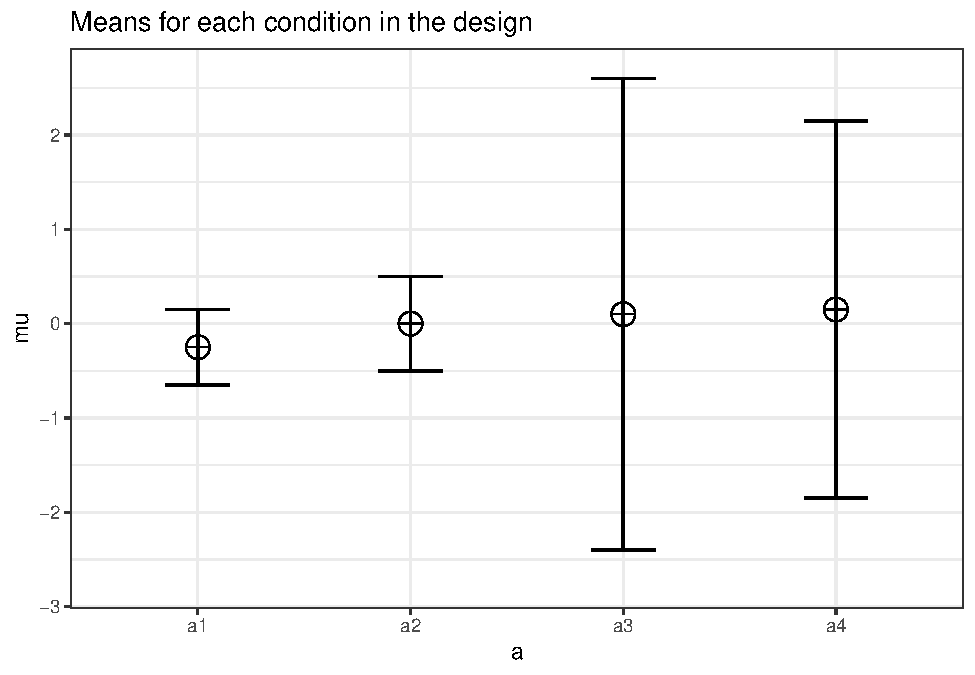
\includegraphics{SuperpowerValidation_files/figure-latex/aberson_6.6-1.pdf}

\begin{Shaded}
\begin{Highlighting}[]
\NormalTok{design_result}\OperatorTok{$}\NormalTok{cor_mat}
\end{Highlighting}
\end{Shaded}

\begin{verbatim}
##     a1  a2  a3  a4
## a1 1.0 0.5 0.3 0.1
## a2 0.5 1.0 0.5 0.3
## a3 0.3 0.5 1.0 0.4
## a4 0.1 0.3 0.4 1.0
\end{verbatim}

There is no analytical result from \texttt{Superpower} when the correlations vary.

Now we prouce 3 \texttt{ANOVA\_exact} results representing no sphericity correction, Greenhouse-Geisser, and Huynh-Feldt corrected results.

\begin{Shaded}
\begin{Highlighting}[]
\NormalTok{exact_result <-}\StringTok{ }\KeywordTok{ANOVA_exact}\NormalTok{(design_result, }\DataTypeTok{verbose =} \OtherTok{FALSE}\NormalTok{)}

\NormalTok{exact_result}\OperatorTok{$}\NormalTok{main_results}
\end{Highlighting}
\end{Shaded}

\begin{verbatim}
##      power partial_eta_squared   cohen_f non_centrality
## a 39.74802          0.01502077 0.1234902       4.529201
\end{verbatim}

\begin{Shaded}
\begin{Highlighting}[]
\NormalTok{exact_result <-}\StringTok{ }\KeywordTok{ANOVA_exact}\NormalTok{(design_result,}
                            \DataTypeTok{correction =} \StringTok{"GG"}\NormalTok{,}
                            \DataTypeTok{verbose =} \OtherTok{FALSE}\NormalTok{)}

\NormalTok{exact_result}\OperatorTok{$}\NormalTok{main_results}
\end{Highlighting}
\end{Shaded}

\begin{verbatim}
##      power partial_eta_squared   cohen_f non_centrality
## a 31.78652          0.01502077 0.1234902       2.997994
\end{verbatim}

\begin{Shaded}
\begin{Highlighting}[]
\NormalTok{exact_result <-}\StringTok{ }\KeywordTok{ANOVA_exact}\NormalTok{(design_result,}
                            \DataTypeTok{correction =} \StringTok{"HF"}\NormalTok{,}
                            \DataTypeTok{verbose =} \OtherTok{FALSE}\NormalTok{)}

\NormalTok{exact_result}\OperatorTok{$}\NormalTok{main_results}
\end{Highlighting}
\end{Shaded}

\begin{verbatim}
##      power partial_eta_squared   cohen_f non_centrality
## a 32.12295          0.01502077 0.1234902       3.059139
\end{verbatim}

And these match \texttt{pwr2ppl}.

\begin{Shaded}
\begin{Highlighting}[]
\KeywordTok{win1F}\NormalTok{(}\DataTypeTok{m1 =} \FloatTok{-.25}\NormalTok{, }\DataTypeTok{m2 =} \FloatTok{.00}\NormalTok{, }\DataTypeTok{m3 =} \FloatTok{.10}\NormalTok{, }\DataTypeTok{m4 =} \FloatTok{.15}\NormalTok{,}
      \DataTypeTok{s1 =} \FloatTok{.4}\NormalTok{, }\DataTypeTok{s2 =} \FloatTok{.5}\NormalTok{, }\DataTypeTok{s3 =} \FloatTok{2.5}\NormalTok{, }\DataTypeTok{s4 =} \FloatTok{2.0}\NormalTok{,}
      \DataTypeTok{r12 =} \FloatTok{.50}\NormalTok{, }\DataTypeTok{r13 =} \FloatTok{.30}\NormalTok{, }\DataTypeTok{r14 =} \FloatTok{.10}\NormalTok{,}
      \DataTypeTok{r23 =} \FloatTok{.5}\NormalTok{, }\DataTypeTok{r24 =} \FloatTok{.30}\NormalTok{, }\DataTypeTok{r34 =} \FloatTok{.40}\NormalTok{,}
      \DataTypeTok{n =} \DecValTok{100}\NormalTok{)}
\end{Highlighting}
\end{Shaded}

\begin{verbatim}
## partial eta-squared = 0.015
\end{verbatim}

\begin{verbatim}
## Power (Unadjusted) for n = 100 is 0.397
\end{verbatim}

\begin{verbatim}
## Power H-F Adjusted (Epsilon = 0.675) for n = 100 is 0.321
\end{verbatim}

\begin{verbatim}
## Power G-G Adjusted (Epsilon = 0.662) for n = 100 is 0.318
\end{verbatim}

\hypertarget{example-from-table-6.8}{%
\subsection{Example from Table 6.8}\label{example-from-table-6.8}}

\begin{Shaded}
\begin{Highlighting}[]
\NormalTok{design_result <-}\StringTok{ }\KeywordTok{ANOVA_design}\NormalTok{(}\DataTypeTok{design =} \StringTok{"2w*4w"}\NormalTok{,}
                              \DataTypeTok{n =} \DecValTok{80}\NormalTok{,}
                              \DataTypeTok{sd =} \KeywordTok{c}\NormalTok{(.}\DecValTok{4}\NormalTok{,}\FloatTok{0.5}\NormalTok{, }
                                     \FloatTok{2.5}\NormalTok{,}\FloatTok{2.0}\NormalTok{, }
                                     \FloatTok{0.4}\NormalTok{,}\FloatTok{0.5}\NormalTok{, }
                                     \FloatTok{2.5}\NormalTok{,}\FloatTok{2.0}\NormalTok{),}
                              \DataTypeTok{mu =} \KeywordTok{c}\NormalTok{(}\OperatorTok{-}\FloatTok{0.25}\NormalTok{,}\FloatTok{0.0}\NormalTok{, }
                                     \FloatTok{0.10}\NormalTok{,}\FloatTok{0.15}\NormalTok{, }
                                     \FloatTok{-0.25}\NormalTok{,}\FloatTok{0.10}\NormalTok{, }
                                     \FloatTok{0.30}\NormalTok{,}\FloatTok{0.35}\NormalTok{),}
                              \DataTypeTok{r =} \KeywordTok{c}\NormalTok{(.}\DecValTok{5}\NormalTok{),}
                              \DataTypeTok{plot =} \OtherTok{TRUE}\NormalTok{)}
\end{Highlighting}
\end{Shaded}

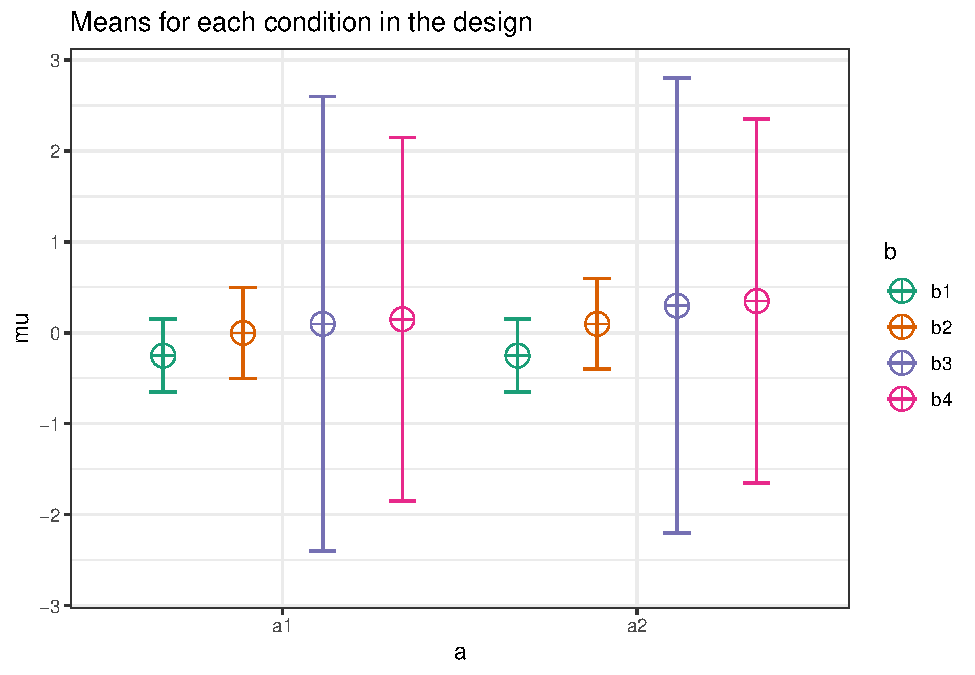
\includegraphics{SuperpowerValidation_files/figure-latex/aberson_6.8-1.pdf}

\begin{Shaded}
\begin{Highlighting}[]
\NormalTok{design_result}\OperatorTok{$}\NormalTok{cor_mat}
\end{Highlighting}
\end{Shaded}

\begin{verbatim}
##       a1_b1 a1_b2 a1_b3 a1_b4 a2_b1 a2_b2 a2_b3 a2_b4
## a1_b1   1.0   0.5   0.5   0.5   0.5   0.5   0.5   0.5
## a1_b2   0.5   1.0   0.5   0.5   0.5   0.5   0.5   0.5
## a1_b3   0.5   0.5   1.0   0.5   0.5   0.5   0.5   0.5
## a1_b4   0.5   0.5   0.5   1.0   0.5   0.5   0.5   0.5
## a2_b1   0.5   0.5   0.5   0.5   1.0   0.5   0.5   0.5
## a2_b2   0.5   0.5   0.5   0.5   0.5   1.0   0.5   0.5
## a2_b3   0.5   0.5   0.5   0.5   0.5   0.5   1.0   0.5
## a2_b4   0.5   0.5   0.5   0.5   0.5   0.5   0.5   1.0
\end{verbatim}

There is no analytical result from \texttt{Superpower} for two-way within subjects designs.

Now we prouce 3 \texttt{ANOVA\_exact} results representing no sphericity correction, Greenhouse-Geisser, and Huynh-Feldt corrected results.

\begin{Shaded}
\begin{Highlighting}[]
\CommentTok{#In comparision to pwr2ppl the main effects are "flipped"}
\CommentTok{# e.g. Superpower a = pwr2ppl "B"}
\NormalTok{exact_result <-}\StringTok{ }\KeywordTok{ANOVA_exact}\NormalTok{(design_result, }\DataTypeTok{verbose =} \OtherTok{FALSE}\NormalTok{)}

\NormalTok{exact_result}\OperatorTok{$}\NormalTok{main_results}
\end{Highlighting}
\end{Shaded}

\begin{verbatim}
##        power partial_eta_squared    cohen_f non_centrality
## a   27.24340         0.023198088 0.15410717      1.8761726
## b   74.84647         0.040077020 0.20432877      9.8948083
## a:b 10.23225         0.003471099 0.05901855      0.8255159
\end{verbatim}

\begin{Shaded}
\begin{Highlighting}[]
\NormalTok{exact_result <-}\StringTok{ }\KeywordTok{ANOVA_exact}\NormalTok{(design_result,}
                            \DataTypeTok{correction =} \StringTok{"GG"}\NormalTok{,}
                            \DataTypeTok{verbose =} \OtherTok{FALSE}\NormalTok{)}

\NormalTok{exact_result}\OperatorTok{$}\NormalTok{main_results}
\end{Highlighting}
\end{Shaded}

\begin{verbatim}
##         power partial_eta_squared    cohen_f non_centrality
## a   27.243403         0.023198088 0.15410717      1.8761726
## b   58.540772         0.040077020 0.20432877      5.9072378
## a:b  9.130272         0.003471099 0.05901855      0.5072161
\end{verbatim}

\begin{Shaded}
\begin{Highlighting}[]
\NormalTok{exact_result <-}\StringTok{ }\KeywordTok{ANOVA_exact}\NormalTok{(design_result,}
                            \DataTypeTok{correction =} \StringTok{"HF"}\NormalTok{,}
                            \DataTypeTok{verbose =} \OtherTok{FALSE}\NormalTok{)}

\NormalTok{exact_result}\OperatorTok{$}\NormalTok{main_results}
\end{Highlighting}
\end{Shaded}

\begin{verbatim}
##         power partial_eta_squared    cohen_f non_centrality
## a   27.243403         0.023198088 0.15410717      1.8761726
## b   59.182337         0.040077020 0.20432877      6.0353398
## a:b  9.174188         0.003471099 0.05901855      0.5187745
\end{verbatim}

And these match \texttt{pwr2ppl}.

\begin{Shaded}
\begin{Highlighting}[]
\KeywordTok{win2F}\NormalTok{(}\DataTypeTok{m1.1 =} \FloatTok{-.25}\NormalTok{, }\DataTypeTok{m2.1 =} \DecValTok{0}\NormalTok{,}
      \DataTypeTok{m3.1 =} \FloatTok{.10}\NormalTok{, }\DataTypeTok{m4.1 =} \FloatTok{.15}\NormalTok{,}
      \DataTypeTok{m1.2 =} \FloatTok{-.25}\NormalTok{, }\DataTypeTok{m2.2 =} \FloatTok{.10}\NormalTok{,}
      \DataTypeTok{m3.2 =} \FloatTok{.30}\NormalTok{, }\DataTypeTok{m4.2 =} \FloatTok{.35}\NormalTok{,}
      \DataTypeTok{s1.1 =} \FloatTok{.4}\NormalTok{, }\DataTypeTok{s2.1 =} \FloatTok{.5}\NormalTok{,}
      \DataTypeTok{s3.1 =} \FloatTok{2.5}\NormalTok{, }\DataTypeTok{s4.1 =} \FloatTok{2.0}\NormalTok{,}
      \DataTypeTok{s1.2 =} \FloatTok{.4}\NormalTok{, }\DataTypeTok{s2.2 =} \FloatTok{.5}\NormalTok{,}
      \DataTypeTok{s3.2 =} \FloatTok{2.5}\NormalTok{, }\DataTypeTok{s4.2 =} \FloatTok{2.0}\NormalTok{,}
      \DataTypeTok{r =} \FloatTok{.5}\NormalTok{, }\DataTypeTok{n =} \DecValTok{80}\NormalTok{)}
\end{Highlighting}
\end{Shaded}

\begin{verbatim}
## Partial eta-squared Factor A = 0.04
\end{verbatim}

\begin{verbatim}
## Power Factor A (Unadjusted) for n = 80 is 0.748
\end{verbatim}

\begin{verbatim}
## Power Factor A H-F Adjusted (Epsilon = 0.61) for n = 80 is 0.592
\end{verbatim}

\begin{verbatim}
## Power Factor A G-G Adjusted (Epsilon = 0.597) for n = 80 is 0.585
\end{verbatim}

\begin{verbatim}
## Partial eta-squared Factor B = 0.023
\end{verbatim}

\begin{verbatim}
## Power Factor B (Unadjusted) for n = 80 is 0.272
\end{verbatim}

\begin{verbatim}
## Power Factor B Adjusted - There is no adjustment when levels = 2
\end{verbatim}

\begin{verbatim}
## Partial eta-squared AxB = 0.003
\end{verbatim}

\begin{verbatim}
## Power AxB (Unadjusted) for n = 80 is 0.102
\end{verbatim}

\begin{verbatim}
## Power AxB H-F Adjusted (Epsilon = 0.628) for n = 80 is 0.092
\end{verbatim}

\begin{verbatim}
## Power AxB G-G Adjusted (Epsilon = 0.614) for n = 80 is 0.091
\end{verbatim}

\hypertarget{example-from-chapter-7}{%
\section{Example from Chapter 7}\label{example-from-chapter-7}}

Mixed effect ANOVA

\hypertarget{from-table-7.2}{%
\subsection{From Table 7.2}\label{from-table-7.2}}

In this case we must write out an entire correlation matrix.
This means the diagonal element is equal to 1 and the off-diagonal elements corresponding to between-subjects factors are equal to zero.

\begin{Shaded}
\begin{Highlighting}[]
\NormalTok{design_result <-}\StringTok{ }\KeywordTok{ANOVA_design}\NormalTok{(}\StringTok{"2b*4w"}\NormalTok{,}
                              \DataTypeTok{n =} \DecValTok{50}\NormalTok{,}
                              \DataTypeTok{sd =} \KeywordTok{c}\NormalTok{(.}\DecValTok{4}\NormalTok{, }\FloatTok{.5}\NormalTok{, }\FloatTok{0.6}\NormalTok{, }\FloatTok{.7}\NormalTok{,}
                                     \FloatTok{.4}\NormalTok{, }\FloatTok{.5}\NormalTok{, }\FloatTok{.6}\NormalTok{, }\FloatTok{.7}\NormalTok{),}
                              \DataTypeTok{r =} \KeywordTok{c}\NormalTok{(}\FloatTok{1.0}\NormalTok{,}\FloatTok{0.5}\NormalTok{,}\FloatTok{0.3}\NormalTok{,}\FloatTok{0.15}\NormalTok{,}\FloatTok{0.0}\NormalTok{,}\FloatTok{0.0}\NormalTok{,}\FloatTok{0.0}\NormalTok{,}\FloatTok{0.0}\NormalTok{,}
                                    \FloatTok{0.5}\NormalTok{,}\FloatTok{1.0}\NormalTok{,}\FloatTok{0.5}\NormalTok{,}\FloatTok{0.3}\NormalTok{,}\FloatTok{0.0}\NormalTok{,}\FloatTok{0.0}\NormalTok{,}\FloatTok{0.0}\NormalTok{,}\FloatTok{0.0}\NormalTok{,}
                                    \FloatTok{0.3}\NormalTok{,}\FloatTok{0.5}\NormalTok{,}\FloatTok{1.0}\NormalTok{,}\FloatTok{0.5}\NormalTok{,}\FloatTok{0.0}\NormalTok{,}\FloatTok{0.0}\NormalTok{,}\FloatTok{0.0}\NormalTok{,}\FloatTok{0.0}\NormalTok{,}
                                    \FloatTok{0.15}\NormalTok{,}\FloatTok{0.3}\NormalTok{,}\FloatTok{0.5}\NormalTok{,}\FloatTok{1.0}\NormalTok{,}\FloatTok{0.0}\NormalTok{,}\FloatTok{0.0}\NormalTok{,}\FloatTok{0.0}\NormalTok{,}\FloatTok{0.0}\NormalTok{,}
                                    \FloatTok{0.0}\NormalTok{,}\FloatTok{0.0}\NormalTok{,}\FloatTok{0.0}\NormalTok{,}\FloatTok{0.0}\NormalTok{,}\FloatTok{1.0}\NormalTok{,}\FloatTok{0.5}\NormalTok{,}\FloatTok{0.3}\NormalTok{,}\FloatTok{0.15}\NormalTok{,}
                                    \FloatTok{0.0}\NormalTok{,}\FloatTok{0.0}\NormalTok{,}\FloatTok{0.0}\NormalTok{,}\FloatTok{0.0}\NormalTok{,}\FloatTok{0.5}\NormalTok{,}\FloatTok{1.0}\NormalTok{,}\FloatTok{0.5}\NormalTok{,}\FloatTok{0.3}\NormalTok{,}
                                    \FloatTok{0.0}\NormalTok{,}\FloatTok{0.0}\NormalTok{,}\FloatTok{0.0}\NormalTok{,}\FloatTok{0.0}\NormalTok{,}\FloatTok{0.3}\NormalTok{,}\FloatTok{0.5}\NormalTok{,}\FloatTok{1.0}\NormalTok{,}\FloatTok{0.5}\NormalTok{,}
                                    \FloatTok{0.0}\NormalTok{,}\FloatTok{0.0}\NormalTok{,}\FloatTok{0.0}\NormalTok{,}\FloatTok{0.0}\NormalTok{,}\FloatTok{0.15}\NormalTok{,}\FloatTok{0.3}\NormalTok{,}\FloatTok{0.5}\NormalTok{,}\FloatTok{1.0}\NormalTok{),}
                              \DataTypeTok{mu =} \KeywordTok{c}\NormalTok{(}\OperatorTok{-}\NormalTok{.}\DecValTok{25}\NormalTok{, }\FloatTok{0.0}\NormalTok{, }\FloatTok{0.10}\NormalTok{, }\FloatTok{0.15}\NormalTok{,}
                                     \FloatTok{-.25}\NormalTok{,}\OperatorTok{-}\NormalTok{.}\DecValTok{25}\NormalTok{,}\OperatorTok{-}\NormalTok{.}\DecValTok{25}\NormalTok{,}\OperatorTok{-}\NormalTok{.}\DecValTok{25}\NormalTok{))}

\NormalTok{design_result}\OperatorTok{$}\NormalTok{cor_mat}
\end{Highlighting}
\end{Shaded}

\begin{verbatim}
##       a1_b1 a1_b2 a1_b3 a1_b4 a2_b1 a2_b2 a2_b3 a2_b4
## a1_b1  1.00   0.5   0.3  0.15  0.00   0.0   0.0  0.00
## a1_b2  0.50   1.0   0.5  0.30  0.00   0.0   0.0  0.00
## a1_b3  0.30   0.5   1.0  0.50  0.00   0.0   0.0  0.00
## a1_b4  0.15   0.3   0.5  1.00  0.00   0.0   0.0  0.00
## a2_b1  0.00   0.0   0.0  0.00  1.00   0.5   0.3  0.15
## a2_b2  0.00   0.0   0.0  0.00  0.50   1.0   0.5  0.30
## a2_b3  0.00   0.0   0.0  0.00  0.30   0.5   1.0  0.50
## a2_b4  0.00   0.0   0.0  0.00  0.15   0.3   0.5  1.00
\end{verbatim}

Now the results from \texttt{ANOVA\_exact}.

\begin{Shaded}
\begin{Highlighting}[]
\NormalTok{exact_result <-}\StringTok{ }\KeywordTok{ANOVA_exact}\NormalTok{(design_result,}
                            \DataTypeTok{correction =} \StringTok{"none"}\NormalTok{,}
                            \DataTypeTok{verbose =} \OtherTok{FALSE}\NormalTok{)}

\NormalTok{exact_result}\OperatorTok{$}\NormalTok{main_results}
\end{Highlighting}
\end{Shaded}

\begin{verbatim}
##        power partial_eta_squared   cohen_f non_centrality
## a   86.42918          0.08878976 0.3121563       9.549274
## b   82.68405          0.03848397 0.2000607      11.767135
## a:b 82.68405          0.03848397 0.2000607      11.767135
\end{verbatim}

\begin{Shaded}
\begin{Highlighting}[]
\NormalTok{exact_result <-}\StringTok{ }\KeywordTok{ANOVA_exact}\NormalTok{(design_result,}
                            \DataTypeTok{correction =} \StringTok{"GG"}\NormalTok{,}
                            \DataTypeTok{verbose =} \OtherTok{FALSE}\NormalTok{)}

\NormalTok{exact_result}\OperatorTok{$}\NormalTok{main_results}
\end{Highlighting}
\end{Shaded}

\begin{verbatim}
##        power partial_eta_squared   cohen_f non_centrality
## a   86.42918          0.08878976 0.3121563       9.549274
## b   76.47495          0.03848397 0.2000607       9.585214
## a:b 76.47495          0.03848397 0.2000607       9.585214
\end{verbatim}

\begin{Shaded}
\begin{Highlighting}[]
\NormalTok{exact_result <-}\StringTok{ }\KeywordTok{ANOVA_exact}\NormalTok{(design_result,}
                            \DataTypeTok{correction =} \StringTok{"HF"}\NormalTok{,}
                            \DataTypeTok{verbose =} \OtherTok{FALSE}\NormalTok{)}

\NormalTok{exact_result}\OperatorTok{$}\NormalTok{main_results}
\end{Highlighting}
\end{Shaded}

\begin{verbatim}
##        power partial_eta_squared   cohen_f non_centrality
## a   86.42918          0.08878976 0.3121563       9.549274
## b   77.31933          0.03848397 0.2000607       9.848557
## a:b 77.31933          0.03848397 0.2000607       9.848557
\end{verbatim}

And the results from \texttt{pwr2ppl}.

\begin{Shaded}
\begin{Highlighting}[]
\KeywordTok{win1bg1}\NormalTok{(}\DataTypeTok{m1.1 =} \FloatTok{-.25}\NormalTok{, }\DataTypeTok{m2.1 =} \DecValTok{0}\NormalTok{, }\DataTypeTok{m3.1 =} \FloatTok{0.10}\NormalTok{, }\DataTypeTok{m4.1 =} \FloatTok{.15}\NormalTok{, }
        \DataTypeTok{m1.2 =} \FloatTok{-.25}\NormalTok{, }\DataTypeTok{m2.2 =} \FloatTok{-.25}\NormalTok{, }\DataTypeTok{m3.2 =} \FloatTok{-.25}\NormalTok{, }\DataTypeTok{m4.2 =} \FloatTok{-.25}\NormalTok{, }
        \DataTypeTok{s1.1 =} \FloatTok{.4}\NormalTok{, }\DataTypeTok{s2.1 =} \FloatTok{.5}\NormalTok{, }\DataTypeTok{s3.1 =} \FloatTok{0.6}\NormalTok{, }\DataTypeTok{s4.1 =} \FloatTok{.7}\NormalTok{, }\DataTypeTok{s1.2 =} \FloatTok{.4}\NormalTok{, }
        \DataTypeTok{s2.2 =} \FloatTok{.5}\NormalTok{, }\DataTypeTok{s3.2 =} \FloatTok{.6}\NormalTok{, }\DataTypeTok{s4.2 =} \FloatTok{.7}\NormalTok{,}
        \DataTypeTok{n =} \DecValTok{50}\NormalTok{, }
        \DataTypeTok{r1.2_1 =} \FloatTok{.5}\NormalTok{, }\DataTypeTok{r1.3_1 =} \FloatTok{.3}\NormalTok{, }\DataTypeTok{r1.4_1 =} \FloatTok{.15}\NormalTok{, }
        \DataTypeTok{r2.3_1 =} \FloatTok{.5}\NormalTok{, }\DataTypeTok{r2.4_1 =} \FloatTok{.3}\NormalTok{, }\DataTypeTok{r3.4_1 =} \FloatTok{.5}\NormalTok{, }
        \DataTypeTok{r1.2_2 =} \FloatTok{.5}\NormalTok{, }\DataTypeTok{r1.3_2 =} \FloatTok{.3}\NormalTok{, }\DataTypeTok{r1.4_2 =} \FloatTok{.15}\NormalTok{, }
        \DataTypeTok{r2.3_2 =} \FloatTok{.5}\NormalTok{, }\DataTypeTok{r2.4_2 =} \FloatTok{.3}\NormalTok{, }\DataTypeTok{r3.4_2 =} \FloatTok{.5}\NormalTok{)}
\end{Highlighting}
\end{Shaded}

\begin{verbatim}
## Partial eta-squared Factor A = 0.089
\end{verbatim}

\begin{verbatim}
## Power Factor A (Between) for n = 50 is 0.864
\end{verbatim}

\begin{verbatim}
## Partial eta-squared Factor B = 0.038
\end{verbatim}

\begin{verbatim}
## Power Factor B (Within) for n = 50 is 0.827
\end{verbatim}

\begin{verbatim}
## Power Factor B H-F Adjusted (Epsilon = 0.837), for n = 50 is 0.773
\end{verbatim}

\begin{verbatim}
## Power Factor B G-G Adjusted (Epsilon = 0.815) for n = 50 is 0.765
\end{verbatim}

\begin{verbatim}
## Partial eta-squared Factor AxB = 0.089
\end{verbatim}

\begin{verbatim}
## Power AxB (Unadjusted) for n = 50 is 0.827
\end{verbatim}

\begin{verbatim}
## Power AxB H-F Adjusted (Epsilon = 0.837) for n = 50 is 0.761
\end{verbatim}

\begin{verbatim}
## Power AxB G-G Adjusted (Epsilon = 0.815) for n = 50 is 0.765
\end{verbatim}

\hypertarget{appendix-2-direct-comparison-to-morepower}{%
\chapter*{Appendix 2: Direct Comparison to MOREpower}\label{appendix-2-direct-comparison-to-morepower}}
\addcontentsline{toc}{chapter}{Appendix 2: Direct Comparison to MOREpower}

MOREpower 6.0 by \citet{Campbell2012MorePower6F} is standalone software for power analysis for ANOVA, t-tests, correlations, and tests of proportions. It outperforms Gpower, in that it allows researchers to perform power analyses for a much wider range of designs. It allows a maximum of 9 levels per factor. Users can solve for N, power or effect size. An ANOVA effect size may be specified in terms of the effect-related variance explained (partial eta-squared) or in terms of a test statistic (\emph{F}, mean square treatment {[}MST{]}, or \emph{t}).

Compared to \texttt{Superpower}, it does not provide all tests at once, it does not provide simple comparisons, it does not incorporate corrections for multiple comparisons, and it does not allow users to enter the means, sd's, and correlations.

We can replicate the independent \emph{t}-test example in MOREpower:

\begin{Shaded}
\begin{Highlighting}[]
\NormalTok{string <-}\StringTok{ "2b"}
\NormalTok{n <-}\StringTok{ }\DecValTok{100}
\NormalTok{mu <-}\StringTok{ }\KeywordTok{c}\NormalTok{(}\DecValTok{24}\NormalTok{, }\FloatTok{26.2}\NormalTok{)}
\NormalTok{sd <-}\StringTok{ }\FloatTok{6.4}
\NormalTok{labelnames <-}\StringTok{ }\KeywordTok{c}\NormalTok{(}\StringTok{"condition"}\NormalTok{, }\StringTok{"control"}\NormalTok{, }\StringTok{"pet"}\NormalTok{) }\CommentTok{#}
\CommentTok{# the label names should be in the order of the means specified above.}
\NormalTok{design_result <-}\StringTok{ }\KeywordTok{ANOVA_design}\NormalTok{(}\DataTypeTok{design =}\NormalTok{ string,}
                              \DataTypeTok{n =}\NormalTok{ n,}
                              \DataTypeTok{mu =}\NormalTok{ mu,}
                              \DataTypeTok{sd =}\NormalTok{ sd,}
                              \DataTypeTok{labelnames =}\NormalTok{ labelnames)}
\NormalTok{alpha_level <-}\StringTok{ }\FloatTok{0.05}

\NormalTok{exact_result <-}\StringTok{ }\KeywordTok{ANOVA_exact}\NormalTok{(design_result,}
                            \DataTypeTok{alpha_level =}\NormalTok{ alpha_level,}
                            \DataTypeTok{verbose =} \OtherTok{TRUE}\NormalTok{)}
\end{Highlighting}
\end{Shaded}

\begin{verbatim}
## Power and Effect sizes for ANOVA tests
##             power partial_eta_squared cohen_f non_centrality
## condition 67.6857               0.029  0.1727         5.9082
## 
## Power and Effect sizes for contrasts
##                                   power effect_size
## p_condition_control_condition_pet 67.69      0.3437
\end{verbatim}

\begin{Shaded}
\begin{Highlighting}[]
\NormalTok{exact_result}\OperatorTok{$}\NormalTok{main_result}\OperatorTok{$}\NormalTok{partial_eta_squared}
\end{Highlighting}
\end{Shaded}

\begin{verbatim}
## [1] 0.02897482
\end{verbatim}

\begin{Shaded}
\begin{Highlighting}[]
\NormalTok{exact_result}\OperatorTok{$}\NormalTok{main_result}\OperatorTok{$}\NormalTok{power}
\end{Highlighting}
\end{Shaded}

\begin{verbatim}
## [1] 67.68572
\end{verbatim}

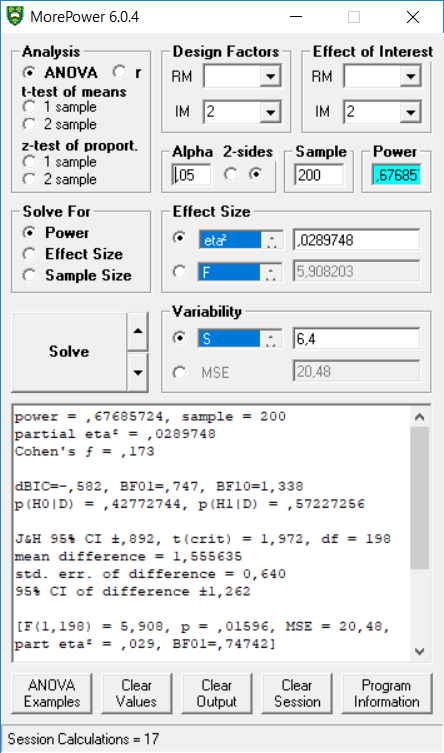
\includegraphics{screenshots/morepower_1.png}

We see the power estimates almost perfectly align with MOREpower if we enter partial eta-squared of 0.02897482, sample = 200 (MOREpower requires entering the total N, not N per condition).

We can also replicate the dependent \emph{t}-test example in MOREpower.

\begin{Shaded}
\begin{Highlighting}[]
\NormalTok{K <-}\StringTok{ }\DecValTok{2}
\NormalTok{n <-}\StringTok{ }\DecValTok{34}
\NormalTok{sd <-}\StringTok{ }\DecValTok{1}
\NormalTok{r <-}\StringTok{ }\FloatTok{0.5}
\NormalTok{alpha =}\StringTok{ }\FloatTok{0.05}
\NormalTok{f <-}\StringTok{ }\FloatTok{0.25}
\NormalTok{f2 <-}\StringTok{ }\NormalTok{f}\OperatorTok{^}\DecValTok{2}
\NormalTok{ES <-}\StringTok{ }\NormalTok{f2}\OperatorTok{/}\NormalTok{(f2 }\OperatorTok{+}\StringTok{ }\DecValTok{1}\NormalTok{)}
\NormalTok{ES}
\end{Highlighting}
\end{Shaded}

\begin{verbatim}
## [1] 0.05882353
\end{verbatim}

\begin{Shaded}
\begin{Highlighting}[]
\NormalTok{mu <-}\StringTok{ }\KeywordTok{mu_from_ES}\NormalTok{(}\DataTypeTok{K =}\NormalTok{ K, }\DataTypeTok{ES =}\NormalTok{ ES)}
\NormalTok{design =}\StringTok{ }\KeywordTok{paste}\NormalTok{(K,}\StringTok{"w"}\NormalTok{,}\DataTypeTok{sep =} \StringTok{""}\NormalTok{)}
\NormalTok{labelnames <-}\StringTok{ }\KeywordTok{c}\NormalTok{(}\StringTok{"speed"}\NormalTok{, }\StringTok{"fast"}\NormalTok{, }\StringTok{"slow"}\NormalTok{)}

\NormalTok{design_result <-}\StringTok{ }\KeywordTok{ANOVA_design}\NormalTok{(}\DataTypeTok{design =}\NormalTok{ design,}
                   \DataTypeTok{n =}\NormalTok{ n, }
                   \DataTypeTok{mu =}\NormalTok{ mu, }
                   \DataTypeTok{sd =}\NormalTok{ sd, }
                   \DataTypeTok{r =}\NormalTok{ r, }
                   \DataTypeTok{labelnames =}\NormalTok{ labelnames)}

\NormalTok{alpha_level <-}\StringTok{ }\FloatTok{0.05}

\NormalTok{exact_result <-}\StringTok{ }\KeywordTok{ANOVA_exact}\NormalTok{(design_result,}
                            \DataTypeTok{alpha_level =}\NormalTok{ alpha_level,}
                            \DataTypeTok{verbose =} \OtherTok{TRUE}\NormalTok{)}
\end{Highlighting}
\end{Shaded}

\begin{verbatim}
## Power and Effect sizes for ANOVA tests
##         power partial_eta_squared cohen_f non_centrality
## speed 80.7778              0.2048  0.5075            8.5
## 
## Power and Effect sizes for contrasts
##                         power effect_size
## p_speed_fast_speed_slow 80.78         0.5
\end{verbatim}

\begin{Shaded}
\begin{Highlighting}[]
\NormalTok{exact_result}\OperatorTok{$}\NormalTok{main_result}\OperatorTok{$}\NormalTok{partial_eta_squared}
\end{Highlighting}
\end{Shaded}

\begin{verbatim}
## [1] 0.2048193
\end{verbatim}

\begin{Shaded}
\begin{Highlighting}[]
\NormalTok{exact_result}\OperatorTok{$}\NormalTok{main_result}\OperatorTok{$}\NormalTok{power}
\end{Highlighting}
\end{Shaded}

\begin{verbatim}
## [1] 80.77775
\end{verbatim}

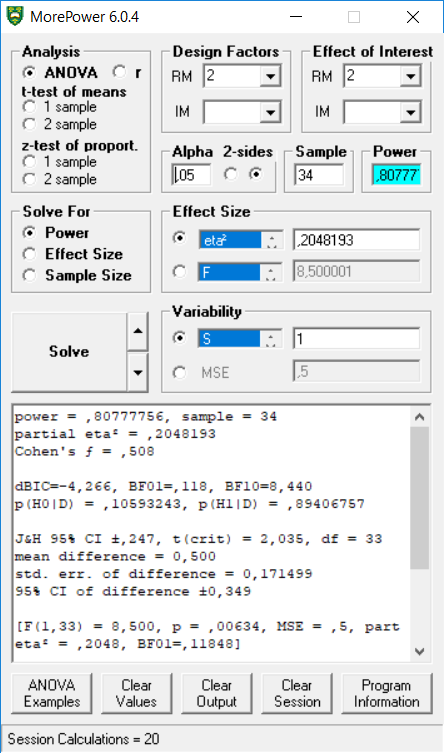
\includegraphics{screenshots/morepower_2.png}

We can also replicate the 3-group within ANOVA example in MOREpower.

\begin{Shaded}
\begin{Highlighting}[]
\NormalTok{K <-}\StringTok{ }\DecValTok{3}
\NormalTok{n <-}\StringTok{ }\DecValTok{20}
\NormalTok{sd <-}\StringTok{ }\DecValTok{1}
\NormalTok{r <-}\StringTok{ }\FloatTok{0.8}
\NormalTok{alpha =}\StringTok{ }\FloatTok{0.05}
\NormalTok{f <-}\StringTok{ }\FloatTok{0.25}
\NormalTok{f2 <-}\StringTok{ }\NormalTok{f}\OperatorTok{^}\DecValTok{2}
\NormalTok{ES <-}\StringTok{ }\NormalTok{f2 }\OperatorTok{/}\StringTok{ }\NormalTok{(f2 }\OperatorTok{+}\StringTok{ }\DecValTok{1}\NormalTok{)}
\NormalTok{ES}
\end{Highlighting}
\end{Shaded}

\begin{verbatim}
## [1] 0.05882353
\end{verbatim}

\begin{Shaded}
\begin{Highlighting}[]
\NormalTok{mu <-}\StringTok{ }\KeywordTok{mu_from_ES}\NormalTok{(}\DataTypeTok{K =}\NormalTok{ K, }\DataTypeTok{ES =}\NormalTok{ ES)}

\NormalTok{design =}\StringTok{ }\KeywordTok{paste}\NormalTok{(K, }\StringTok{"w"}\NormalTok{, }\DataTypeTok{sep =} \StringTok{""}\NormalTok{)}
\NormalTok{labelnames <-}\StringTok{ }\KeywordTok{c}\NormalTok{(}\StringTok{"speed"}\NormalTok{, }\StringTok{"fast"}\NormalTok{, }\StringTok{"medium"}\NormalTok{, }\StringTok{"slow"}\NormalTok{)}
\NormalTok{design_result <-}\StringTok{ }\KeywordTok{ANOVA_design}\NormalTok{(}\DataTypeTok{design =}\NormalTok{ design,}
                   \DataTypeTok{n =}\NormalTok{ n, }
                   \DataTypeTok{mu =}\NormalTok{ mu, }
                   \DataTypeTok{sd =}\NormalTok{ sd, }
                   \DataTypeTok{r =}\NormalTok{ r, }
                   \DataTypeTok{labelnames =}\NormalTok{ labelnames)}

\NormalTok{alpha_level <-}\StringTok{ }\FloatTok{0.05}

\NormalTok{exact_result <-}\StringTok{ }\KeywordTok{ANOVA_exact}\NormalTok{(design_result,}
                            \DataTypeTok{alpha_level =}\NormalTok{ alpha_level,}
                            \DataTypeTok{verbose =} \OtherTok{TRUE}\NormalTok{)}
\end{Highlighting}
\end{Shaded}

\begin{verbatim}
## Power and Effect sizes for ANOVA tests
##         power partial_eta_squared cohen_f non_centrality
## speed 96.9163              0.3304  0.7024          18.75
## 
## Power and Effect sizes for contrasts
##                           power effect_size
## p_speed_fast_speed_medium 53.79      0.4841
## p_speed_fast_speed_slow   98.39      0.9682
## p_speed_medium_speed_slow 53.79      0.4841
\end{verbatim}

\begin{Shaded}
\begin{Highlighting}[]
\CommentTok{#MSE, for MOREpower}
\NormalTok{exact_result[[}\StringTok{"aov_result"}\NormalTok{]][[}\StringTok{"anova_table"}\NormalTok{]]}
\end{Highlighting}
\end{Shaded}

\begin{verbatim}
## Anova Table (Type 3 tests)
## 
## Response: y
##       num Df den Df MSE     F    pes    Pr(>F)    
## speed      2     38 0.2 9.375 0.3304 0.0004904 ***
## ---
## Signif. codes:  0 '***' 0.001 '**' 0.01 '*' 0.05 '.' 0.1 ' ' 1
\end{verbatim}

\begin{Shaded}
\begin{Highlighting}[]
\CommentTok{#POWER}
\NormalTok{exact_result}\OperatorTok{$}\NormalTok{main_result}\OperatorTok{$}\NormalTok{power}
\end{Highlighting}
\end{Shaded}

\begin{verbatim}
## [1] 96.91634
\end{verbatim}

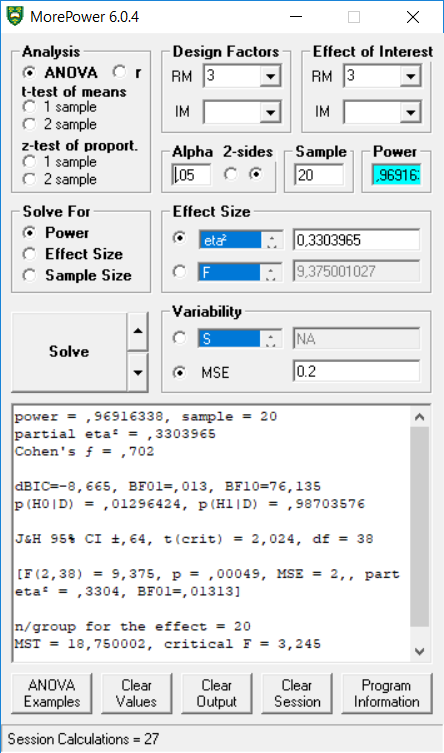
\includegraphics{screenshots/morepower_3.png}

We can reproduce the 2x2 ANOVA example in MOREpower.

\begin{Shaded}
\begin{Highlighting}[]
\NormalTok{mu =}\StringTok{ }\KeywordTok{c}\NormalTok{(}\DecValTok{700}\NormalTok{, }\DecValTok{670}\NormalTok{, }\DecValTok{670}\NormalTok{, }\DecValTok{700}\NormalTok{) }
\NormalTok{sigma =}\StringTok{ }\DecValTok{150}  \CommentTok{# population standard deviation}
\NormalTok{n <-}\StringTok{ }\DecValTok{25}
\NormalTok{sd <-}\StringTok{ }\DecValTok{150}
\NormalTok{r <-}\StringTok{ }\FloatTok{0.75}
\NormalTok{string =}\StringTok{ "2w*2w"}
\NormalTok{alpha_level <-}\StringTok{ }\FloatTok{0.05}
\NormalTok{labelnames =}\StringTok{ }\KeywordTok{c}\NormalTok{(}\StringTok{"age"}\NormalTok{, }\StringTok{"old"}\NormalTok{, }\StringTok{"young"}\NormalTok{, }\StringTok{"color"}\NormalTok{, }\StringTok{"blue"}\NormalTok{, }\StringTok{"red"}\NormalTok{)}
\NormalTok{design_result <-}\StringTok{ }\KeywordTok{ANOVA_design}\NormalTok{(}\DataTypeTok{design =}\NormalTok{ string,}
                              \DataTypeTok{n =}\NormalTok{ n, }
                              \DataTypeTok{mu =}\NormalTok{ mu, }
                              \DataTypeTok{sd =}\NormalTok{ sd, }
                              \DataTypeTok{r =}\NormalTok{ r, }
                              \DataTypeTok{labelnames =}\NormalTok{ labelnames)}

\NormalTok{simulation_result <-}\StringTok{ }\KeywordTok{ANOVA_exact}\NormalTok{(design_result, }
                                 \DataTypeTok{alpha_level =}\NormalTok{ alpha_level, }
                                 \DataTypeTok{verbose =} \OtherTok{TRUE}\NormalTok{)}
\end{Highlighting}
\end{Shaded}

\begin{verbatim}
## Power and Effect sizes for ANOVA tests
##             power partial_eta_squared cohen_f non_centrality
## age        5.0000              0.0000  0.0000              0
## color      5.0000              0.0000  0.0000              0
## age:color 48.4018              0.1429  0.4082              4
## 
## Power and Effect sizes for contrasts
##                                            power effect_size
## p_age_old_color_blue_age_old_color_red      27.4     -0.2828
## p_age_old_color_blue_age_young_color_blue   27.4     -0.2828
## p_age_old_color_blue_age_young_color_red     5.0      0.0000
## p_age_old_color_red_age_young_color_blue     5.0      0.0000
## p_age_old_color_red_age_young_color_red     27.4      0.2828
## p_age_young_color_blue_age_young_color_red  27.4      0.2828
\end{verbatim}

\begin{Shaded}
\begin{Highlighting}[]
\NormalTok{simulation_result}\OperatorTok{$}\NormalTok{main_result}\OperatorTok{$}\NormalTok{partial_eta_squared[}\DecValTok{3}\NormalTok{]}
\end{Highlighting}
\end{Shaded}

\begin{verbatim}
## [1] 0.1428571
\end{verbatim}

This result reproduces the analysis in MOREpower, for a 2x2 within design, with a sample of 25, and eta-squared of 0.1428571.

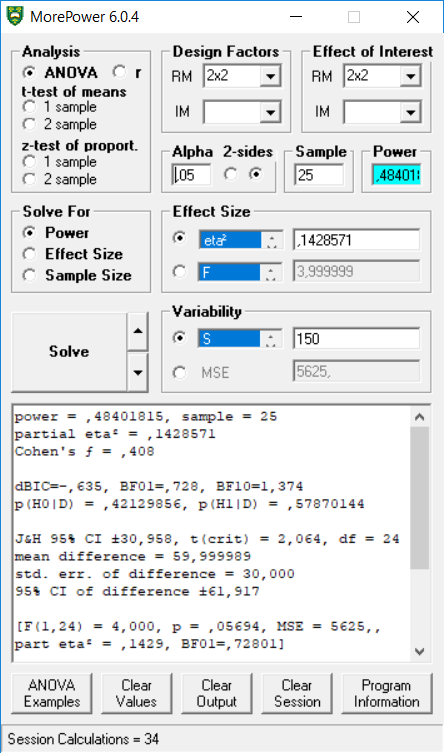
\includegraphics{screenshots/morepower_4.png}

Let's replicate the 2x2x2 full between analysis (total N = 400, effects sizes differ for each test):

\begin{Shaded}
\begin{Highlighting}[]
\CommentTok{# With 2x2x2 designs,}
\CommentTok{# the names for paired comparisons can become very long.}
\CommentTok{# So here I abbreviate terms:}
\CommentTok{# Size, Color, and Cognitive Load, have values:}
\CommentTok{# b = big, s = small, g = green,}
\CommentTok{# r = red, pres = present, abs = absent.}
\NormalTok{labelnames <-}\StringTok{ }\KeywordTok{c}\NormalTok{(}\StringTok{"Size"}\NormalTok{, }\StringTok{"b"}\NormalTok{, }\StringTok{"s"}\NormalTok{, }\StringTok{"Color"}\NormalTok{, }\StringTok{"g"}\NormalTok{, }\StringTok{"r"}\NormalTok{,}
                \StringTok{"Load"}\NormalTok{, }\StringTok{"pres"}\NormalTok{, }\StringTok{"abs"}\NormalTok{) }\CommentTok{#}
\NormalTok{design_result <-}\StringTok{ }\KeywordTok{ANOVA_design}\NormalTok{(}\DataTypeTok{design =} \StringTok{"2b*2b*2b"}\NormalTok{,}
                              \CommentTok{#sample size per group}
                              \DataTypeTok{n =} \DecValTok{50}\NormalTok{,}
                              \CommentTok{#pattern of means}
                              \DataTypeTok{mu =} \KeywordTok{c}\NormalTok{(}\DecValTok{2}\NormalTok{, }\DecValTok{2}\NormalTok{, }\DecValTok{6}\NormalTok{, }\DecValTok{1}\NormalTok{, }\DecValTok{6}\NormalTok{, }\DecValTok{6}\NormalTok{, }\DecValTok{1}\NormalTok{, }\DecValTok{8}\NormalTok{),}
                              \DataTypeTok{sd =} \DecValTok{10}\NormalTok{, }\CommentTok{#standard deviation}
                              \DataTypeTok{labelnames =}\NormalTok{ labelnames)}

\NormalTok{exact_result <-}\StringTok{ }\KeywordTok{ANOVA_exact}\NormalTok{(design_result,}
                            \DataTypeTok{alpha_level =}\NormalTok{ alpha_level,}
                            \DataTypeTok{verbose =} \OtherTok{TRUE}\NormalTok{)}
\end{Highlighting}
\end{Shaded}

\begin{verbatim}
## Power and Effect sizes for ANOVA tests
##                   power partial_eta_squared cohen_f non_centrality
## Size            70.3301              0.0157  0.1263           6.25
## Color            5.0000              0.0000  0.0000           0.00
## Load             7.8953              0.0006  0.0253           0.25
## Size:Color      32.1727              0.0057  0.0758           2.25
## Size:Load       84.9123              0.0224  0.1515           9.00
## Color:Load       7.8953              0.0006  0.0253           0.25
## Size:Color:Load 84.9123              0.0224  0.1515           9.00
## 
## Power and Effect sizes for contrasts
##                                                     power effect_size
## p_Size_b_Color_g_Load_pres_Size_b_Color_g_Load_abs   5.00         0.0
## p_Size_b_Color_g_Load_pres_Size_b_Color_r_Load_pres 50.82         0.4
## p_Size_b_Color_g_Load_pres_Size_b_Color_r_Load_abs   7.85        -0.1
## p_Size_b_Color_g_Load_pres_Size_s_Color_g_Load_pres 50.82         0.4
## p_Size_b_Color_g_Load_pres_Size_s_Color_g_Load_abs  50.82         0.4
## p_Size_b_Color_g_Load_pres_Size_s_Color_r_Load_pres  7.85        -0.1
## p_Size_b_Color_g_Load_pres_Size_s_Color_r_Load_abs  84.39         0.6
## p_Size_b_Color_g_Load_abs_Size_b_Color_r_Load_pres  50.82         0.4
## p_Size_b_Color_g_Load_abs_Size_b_Color_r_Load_abs    7.85        -0.1
## p_Size_b_Color_g_Load_abs_Size_s_Color_g_Load_pres  50.82         0.4
## p_Size_b_Color_g_Load_abs_Size_s_Color_g_Load_abs   50.82         0.4
## p_Size_b_Color_g_Load_abs_Size_s_Color_r_Load_pres   7.85        -0.1
## p_Size_b_Color_g_Load_abs_Size_s_Color_r_Load_abs   84.39         0.6
## p_Size_b_Color_r_Load_pres_Size_b_Color_r_Load_abs  69.69        -0.5
## p_Size_b_Color_r_Load_pres_Size_s_Color_g_Load_pres  5.00         0.0
## p_Size_b_Color_r_Load_pres_Size_s_Color_g_Load_abs   5.00         0.0
## p_Size_b_Color_r_Load_pres_Size_s_Color_r_Load_pres 69.69        -0.5
## p_Size_b_Color_r_Load_pres_Size_s_Color_r_Load_abs  16.77         0.2
## p_Size_b_Color_r_Load_abs_Size_s_Color_g_Load_pres  69.69         0.5
## p_Size_b_Color_r_Load_abs_Size_s_Color_g_Load_abs   69.69         0.5
## p_Size_b_Color_r_Load_abs_Size_s_Color_r_Load_pres   5.00         0.0
## p_Size_b_Color_r_Load_abs_Size_s_Color_r_Load_abs   93.39         0.7
## p_Size_s_Color_g_Load_pres_Size_s_Color_g_Load_abs   5.00         0.0
## p_Size_s_Color_g_Load_pres_Size_s_Color_r_Load_pres 69.69        -0.5
## p_Size_s_Color_g_Load_pres_Size_s_Color_r_Load_abs  16.77         0.2
## p_Size_s_Color_g_Load_abs_Size_s_Color_r_Load_pres  69.69        -0.5
## p_Size_s_Color_g_Load_abs_Size_s_Color_r_Load_abs   16.77         0.2
## p_Size_s_Color_r_Load_pres_Size_s_Color_r_Load_abs  93.39         0.7
\end{verbatim}

\begin{Shaded}
\begin{Highlighting}[]
\NormalTok{exact_result}\OperatorTok{$}\NormalTok{main_result}\OperatorTok{$}\NormalTok{partial_eta_squared}
\end{Highlighting}
\end{Shaded}

\begin{verbatim}
## [1] 0.0156936598 0.0000000000 0.0006373486 0.0057070387 0.0224438903
## [6] 0.0006373486 0.0224438903
\end{verbatim}

This result is nicely reproduced in MOREpower, both for the 2x2 effects, and the 2x2x2 between effects.

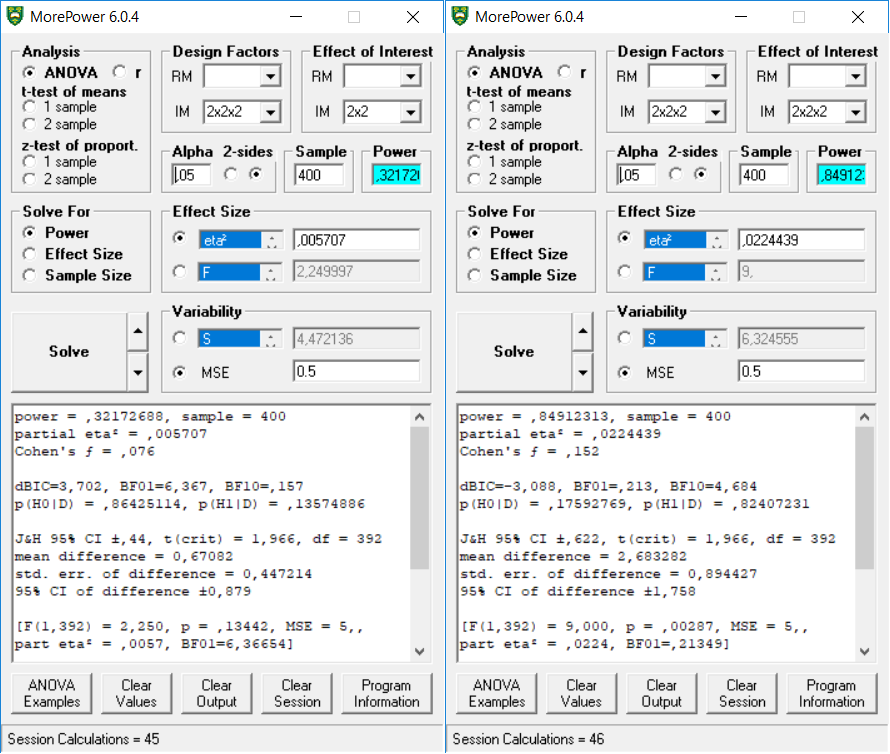
\includegraphics{screenshots/morepower_5.png}

And finally, let's replicate the 2x2 full within analysis.

\begin{Shaded}
\begin{Highlighting}[]
\NormalTok{mu =}\StringTok{ }\KeywordTok{c}\NormalTok{(}\DecValTok{2}\NormalTok{,}\DecValTok{1}\NormalTok{,}\DecValTok{4}\NormalTok{,}\DecValTok{2}\NormalTok{)}
\NormalTok{n <-}\StringTok{ }\DecValTok{20}
\NormalTok{sd <-}\StringTok{ }\DecValTok{5}
\NormalTok{r <-}\StringTok{ }\KeywordTok{c}\NormalTok{(}
  \FloatTok{0.8}\NormalTok{, }\FloatTok{0.5}\NormalTok{, }\FloatTok{0.4}\NormalTok{,}
  \FloatTok{0.4}\NormalTok{, }\FloatTok{0.5}\NormalTok{,}
  \FloatTok{0.8}
\NormalTok{)}
\NormalTok{string =}\StringTok{ "2w*2w"}
\NormalTok{labelnames =}\StringTok{ }\KeywordTok{c}\NormalTok{(}\StringTok{"A"}\NormalTok{, }\StringTok{"a1"}\NormalTok{, }\StringTok{"a2"}\NormalTok{, }\StringTok{"B"}\NormalTok{, }\StringTok{"b1"}\NormalTok{, }\StringTok{"b2"}\NormalTok{)}
\NormalTok{design_result <-}\StringTok{ }\KeywordTok{ANOVA_design}\NormalTok{(}\DataTypeTok{design =}\NormalTok{ string,}
                              \DataTypeTok{n =}\NormalTok{ n,}
                              \DataTypeTok{mu =}\NormalTok{ mu,}
                              \DataTypeTok{sd =}\NormalTok{ sd,}
                              \DataTypeTok{r =}\NormalTok{ r,}
                              \DataTypeTok{labelnames =}\NormalTok{ labelnames)}
\NormalTok{exact_result <-}\StringTok{ }\KeywordTok{ANOVA_exact}\NormalTok{(design_result,}
                            \DataTypeTok{alpha_level =}\NormalTok{ alpha_level,}
                            \DataTypeTok{verbose =} \OtherTok{TRUE}\NormalTok{)}
\end{Highlighting}
\end{Shaded}

\begin{verbatim}
## Power and Effect sizes for ANOVA tests
##       power partial_eta_squared cohen_f non_centrality
## A   26.9175              0.0952  0.3244              2
## B   64.2259              0.2400  0.5620              6
## A:B 26.9175              0.0952  0.3244              2
## 
## Power and Effect sizes for contrasts
##                       power effect_size
## p_A_a1_B_b1_A_a1_B_b2 26.92     -0.3162
## p_A_a1_B_b1_A_a2_B_b1 39.70      0.4000
## p_A_a1_B_b1_A_a2_B_b2  5.00      0.0000
## p_A_a1_B_b2_A_a2_B_b1 64.23      0.5477
## p_A_a1_B_b2_A_a2_B_b2 13.60      0.2000
## p_A_a2_B_b1_A_a2_B_b2 76.52     -0.6325
\end{verbatim}

\begin{Shaded}
\begin{Highlighting}[]
\NormalTok{exact_result}\OperatorTok{$}\NormalTok{main_result}\OperatorTok{$}\NormalTok{partial_eta_squared}
\end{Highlighting}
\end{Shaded}

\begin{verbatim}
## [1] 0.0952381 0.2400000 0.0952381
\end{verbatim}

\begin{Shaded}
\begin{Highlighting}[]
\NormalTok{exact_result}\OperatorTok{$}\NormalTok{main_result}\OperatorTok{$}\NormalTok{power}
\end{Highlighting}
\end{Shaded}

\begin{verbatim}
## [1] 26.91752 64.22587 26.91752
\end{verbatim}

This result is also reproduced in MOREpower, both for the main effect, and the 2x2 within interaction effect.

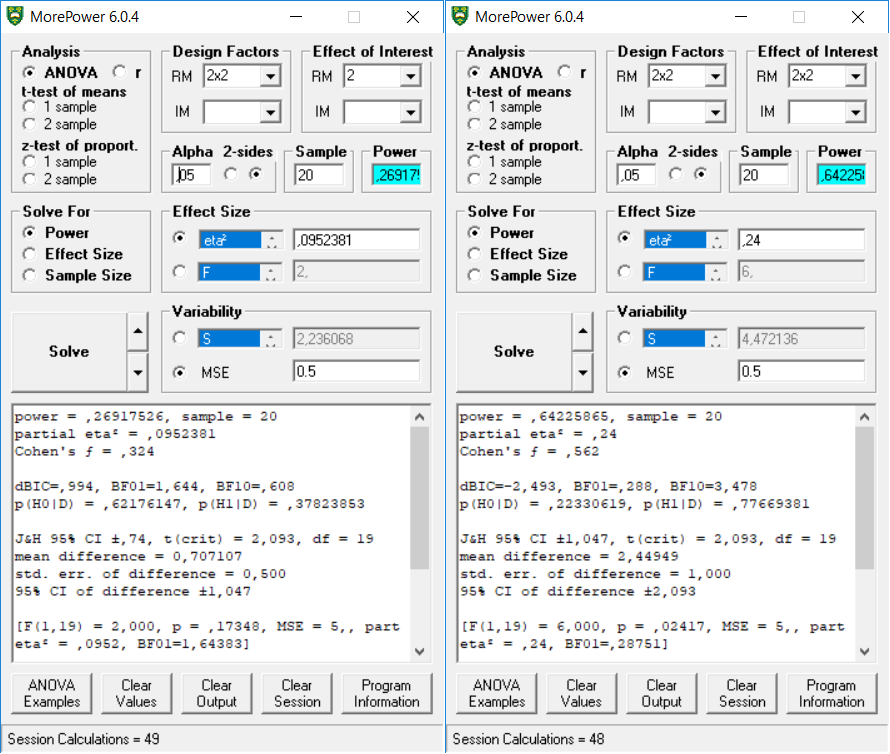
\includegraphics{screenshots/morepower_6.png}

\bibliography{book.bib,packages.bib,references.bib}


\end{document}
